\documentclass[11pt,a4paper]{article}
\usepackage{fontspec}
\IfFontExistsTF{Latin Modern Roman}{\setmainfont{Latin Modern Roman}}{\setmainfont{Liberation Serif}}
\IfFontExistsTF{Latin Modern Sans}{\setsansfont{Latin Modern Sans}}{\setsansfont{Liberation Sans}}
\setmonofont{DejaVu Sans Mono}[Scale=0.79]
\usepackage[a4paper,margin=26mm,headheight=15pt]{geometry}
\usepackage{amsmath,amssymb,amsthm,mathtools}
\usepackage{array,longtable,booktabs,enumitem,xcolor,microtype}
\usepackage{needspace}

\usepackage[unicode,pdfencoding=auto]{hyperref}
\usepackage{xurl}
\usepackage{tikz}
\usetikzlibrary{positioning,arrows.meta}
\definecolor{inkblue}{RGB}{25,54,78}
\hypersetup{colorlinks=true,linkcolor=inkblue,urlcolor=inkblue,citecolor=inkblue,
 pdftitle={Fr\"ohlich Hamiltonian: detailed proofs and dependencies for Lean formalization},
 pdfauthor={Mathematical proof development},bookmarksnumbered=true}
\newtheorem{target}{Target}
\newtheorem{theorem}{Theorem}[section]
\newtheorem{lemma}[theorem]{Lemma}
\newtheorem{proposition}[theorem]{Proposition}
\newtheorem{corollary}[theorem]{Corollary}
\theoremstyle{definition}
\newtheorem{definition}[theorem]{Definition}
\theoremstyle{remark}
\newtheorem{remark}[theorem]{Remark}
\newcommand{\proofid}[1]{\par\smallskip{\normalfont\scriptsize\color{inkblue}Stable ID: \nolinkurl{#1}}\par\smallskip}
\setlength{\parskip}{0.25em}
\setlength{\emergencystretch}{3em}
\setcounter{tocdepth}{2}
\setlist{itemsep=0.35em,topsep=0.5em}
\begin{document}
\hypersetup{pageanchor=false}
\begin{titlepage}
\thispagestyle{empty}
\setlength{\parindent}{0pt}
\vspace*{13mm}
{\sffamily\color{inkblue}\large MATHEMATICAL PROOF BLUEPRINT / REVISION 10}\par
\vspace{12mm}
{\sffamily\bfseries\Huge The three-dimensional\\[2mm] Fr\"ohlich Hamiltonian}\par
\vspace{6mm}
{\sffamily\LARGE Complete mathematical development,\\[3mm]
with explicit domains and dependencies}\par
\vspace{15mm}
\noindent\rule{\textwidth}{0.7pt}\par
\vspace{6mm}
{\large An expanded companion to Griesemer--W\"unsch,\\
\emph{Self-Adjointness and Domain of the Fr\"ohlich Hamiltonian},\\
arXiv:1508.02533v2}\par
\vspace{12mm}
\noindent\textbf{Scope}\quad Mathematical preparation for existence and form domain,
exact operator domain, and sharp regularity in three dimensions.\par
\vspace{4mm}
\noindent\textbf{Foundation}\quad Mathlib-only mathematical leaves, with exact reference names;
proved operator and Fock lemmas; shared prerequisite trees.\par
\vspace{4mm}
\noindent\textbf{Status}\quad Mathematical proof blueprint with source-level reference audit.
No Lean code or kernel-checked formalization is included.\par
\vfill
{\sffamily 10 November 2026}\par
\end{titlepage}
\hypersetup{pageanchor=true}
\pagenumbering{roman}
\begingroup
\small
\setlength{\parskip}{0pt}
\tableofcontents
\endgroup
\clearpage
\pagenumbering{arabic}

% ===== BEGIN PART: 01_targets =====
\section{The three-dimensional model and the three main results}
\label{sec:targets}

This manuscript gives detailed mathematical proofs for the particular
three-dimensional Fr\"ohlich Hamiltonian of Griesemer--W\"unsch~\cite{GW16},
with its coupling constant retained. The later Lean formalization has
exactly three main targets: existence with the correct form domain, the
Gross-transform description of the operator domain, and sharp electron
regularity. Every target is proved by the later named results. A target
statement is a specification, never an input axiom.

The supporting operator, measure, and Fock lemmas are stated at the
generality needed for their proofs. The Hamiltonian itself always has
the fixed form factor below and always lives in three spatial dimensions.

\subsection{Fixed model, coupling, and domain conventions}
\label{target:common-data}

Let $\alpha\in\mathbb R$ with $\alpha\geq0$. We use exactly the coupling
normalization of equation (1) in the source paper:
\[
 v_\alpha(k)=\begin{cases}\sqrt\alpha/|k|,&k\in\mathbb R^3\setminus\{0\},\\
                          0,&k=0.
             \end{cases}
\]
The value at zero is immaterial for all $L^2$ classes and integrals.
The complex one-phonon space is $\mathfrak h=L^2(\mathbb R^3;\mathbb C)$.
Its bosonic Fock space is
$\mathcal F=\bigoplus_{n\geq0}^{\ell^2}\mathcal F_n$, where
$\mathcal F_n$ is the closed symmetric subspace of
$L^2((\mathbb R^3)^n)$ and $\mathcal F_0=\mathbb C$.
The full Hilbert space is
$\mathcal H=L^2(\mathbb R^3_x;\mathcal F)$.
The unitary identification with its particle-sector model is proved below.

Electron momentum is $p=-i\nabla_x$. In the electron Fourier/sector
representation all the following operators have their maximal multiplier
domains:
\[
 p_j\leftrightarrow q_j\ (j=1,2,3),\quad
 |p|^s\leftrightarrow |q|^s,\quad N\leftrightarrow n,\quad
 H_0=p^2+N\leftrightarrow |q|^2+n.
\]
The zeroth power is the identity. In particular,
\[
 D(H_0)=D(p^2)\cap D(N),\qquad
 Q=D(|p|)\cap D(N^{1/2}),\qquad
 \|u\|_Q=\|(H_0+1)^{1/2}u\|.
\]
The free powers in this expression are explicit multipliers. The free
form is
\[
 q_0(u,w)=\sum_{j=1}^3\langle p_ju,p_jw\rangle
                    +\langle N^{1/2}u,N^{1/2}w\rangle,\qquad u,w\in Q.
\]
For $0<\Lambda<\infty$, set
\[
 G_{\alpha,\Lambda,x}(k)=e^{-ik\cdot x}v_\alpha(k)\mathbf1_{|k|\leq\Lambda},
 \qquad H_{\alpha,\Lambda}=H_0+\phi(G_{\alpha,\Lambda})
                                      \quad\text{on }D(H_0),
\]
where $\phi(F)=a(F)+a^*(F)$. The expression at infinite cutoff defines
the interaction through its quadratic form. Ordinary creation with
the coefficient $v_\alpha$ is not asserted when $\alpha>0$.

\paragraph{Conventions for a faithful formal statement.}
Inner products are conjugate-linear in the first variable. Annihilation
is conjugate-linear in its coefficient; creation is linear. The physical
electron Fourier transform has phase $e^{-iq\cdot x}$ and factor
$(2\pi)^{-3/2}$; Lemma~\ref{basic:fourier} relates it to mathlib's convention.
The symbol $\mathbb R^3$ means Euclidean three-space with its Euclidean
norm and Lebesgue measure. In Lean it should be modeled by Euclidean
space on three coordinates; a raw function space's default norm must not
silently replace the Euclidean norm.

All $L^2$ expressions descend to almost-everywhere equivalence classes.
Nonnegative integrals whose finiteness has not been proved have values
in $[0,+\infty]$. An assertion of divergence is about this extended
nonnegative integral, not mathlib's total real-valued Bochner integral.
Every conversion to a real integral carries a finiteness proof.

An unbounded operator includes its linear domain. Every composition
requires both domain memberships. A designated maximal joint multiplier,
such as $N^{1/2}(1+p^2)^{1/2}$, instead has the maximal domain of the
product multiplier; its domain must not be confused with a sequential
composition domain. Operator cores are linear subspaces dense in graph
norm. Their approximation properties are supporting lemmas in the proofs.

\subsection{Main result 1: existence and form domain}

\begin{target}[The self-adjoint Fr\"ohlich Hamiltonian and its form domain]
\label{target:construction}
For every $\alpha\geq0$, the limit
\[
 w_\alpha(u,w)=\lim_{\Lambda\to\infty}
       \langle u,\phi(G_{\alpha,\Lambda})w\rangle,\qquad u,w\in Q,
\]
exists in the norm of bounded sesquilinear forms on $Q$.
The form $q_\alpha=q_0+w_\alpha$ is densely defined, closed, and bounded
below, and its form domain is exactly $Q$.
There exists a unique self-adjoint, bounded-below operator $H_\alpha$
associated with this form. Thus
\[
 \boxed{\ \mathcal Q(H_\alpha)=Q=D(|p|)\cap D(N^{1/2}).\ }
\]
Here $\mathcal Q(H_\alpha)$ is the energy/form domain, equipped with an
equivalent shifted form norm. In particular, $H_{\alpha=0}=H_0$.
\end{target}

\paragraph{Proof location and scope.}
The fixed-coupling estimates are proved in
Lemma~\ref{model:frohlich-estimates}. Lemmas~\ref{main:uv-form} and
\ref{main:uniform-form-bound} construct the form limit, and
Theorem~\ref{main:form-H} applies the proved form-representation theorem.
The interacting \emph{operator} domain is the subject of Main result 2.
Finite-cutoff self-adjointness supports the conjugation calculation.
The limiting dressed operator is identified directly by equality of
mixed forms and the form-representation domain witnesses; no
norm-resolvent convergence theorem is needed for the three targets.

\subsection{Main result 2: the exact operator domain}

\begin{target}[Gross conjugation and the operator domain]
\label{target:domain}
Fix $\alpha\geq0$. There is $K_0(\alpha)>0$ such that, for every
$K\geq K_0(\alpha)$, the following construction has the stated properties.
Put
\[
 b_{\alpha,K}(k)=-\frac{v_\alpha(k)\mathbf1_{|k|>K}}{1+|k|^2},\qquad
 B_{\alpha,K,x}(k)=e^{-ik\cdot x}b_{\alpha,K}(k),\qquad
 (U_{\alpha,K}u)(x)=W(-B_{\alpha,K,x})u(x).
\]
The Weyl convention is
\[
 W(f)E(g)=e^{-\|f\|^2/2-\langle f,g\rangle}E(f+g),\qquad
 E(g)_n=g^{\otimes n}/\sqrt{n!}.
\]
On the full domain $D(H_0)$ define
\begin{align*}
 H'_{\alpha,K}&=H_0+\phi(G_{\alpha,K})+V_{\alpha,K},\\
 V_{\alpha,K}&=-2a^*(kB_{\alpha,K})\cdot p
               -2p\cdot a(kB_{\alpha,K})
               +\sum_{j=1}^3\phi(k_jB_{\alpha,K})^2+C_{\alpha,K},\\
 C_{\alpha,K}&=\int_{|k|>K}|v_\alpha(k)|^2
             \bigl((1+|k|^2)^{-2}-2(1+|k|^2)^{-1}\bigr)\,dk.
\end{align*}
All products in this formula are defined on every $u\in D(H_0)$;
in particular $a(k_jB_{\alpha,K})u\in D(p_j)$ for $j=1,2,3$.
The operator $H'_{\alpha,K}$ is self-adjoint on $D(H_0)$ and its graph
norm is equivalent to the free graph norm. Both $U_{\alpha,K}$ and its
adjoint preserve $Q$. Finally,
\[
 \boxed{\ H_\alpha=U_{\alpha,K}^*H'_{\alpha,K}U_{\alpha,K},\qquad
 D(H_\alpha)=U_{\alpha,K}^*D(H_0).\ }
\]
These are equalities of operators with their full domains. They describe
the same $H_\alpha$ for every sufficiently large choice of $K$.
\end{target}

\paragraph{Proof location.}
The Gross form-domain and finite-cutoff identities are
Lemma~\ref{main:gross-form} and Proposition~\ref{main:conjugation}.
Lemmas~\ref{main:singular-annihilation-limit} and
\ref{main:derivative-annihilation} justify the singular differentiated
term. Theorem~\ref{main:dressed-small} gives self-adjointness;
Theorem~\ref{main:domain} identifies the limiting operator and its domain.
Core approximation and core transfer appear inside this proof chain.

\subsection{Main result 3: sharp electron regularity}

\begin{target}[The sharp $3/2$ momentum threshold]
\label{target:regularity}
For every $\alpha\geq0$,
\[
 D(H_\alpha)\subseteq D(N)\cap
             \bigcap_{0\leq s<3/2}D(|p|^s).
\]
For every $\alpha>0$,
\[
 \boxed{\ D(H_\alpha)\cap D(|p|^{3/2})=\{0\}.\ }
\]
Consequently the same trivial-intersection statement holds with
$D(|p|^s)$ for every $s\geq3/2$, and in particular
$D(H_\alpha)\cap D(p^2)=D(H_\alpha)\cap D(H_0)=\{0\}$.
Equivalently,
\[
 D(H_\alpha)\subseteq D(N)\cap
           \bigcap_{0\leq t<3/4}D((-\Delta)^t),\qquad
 D(H_\alpha)\cap D((-\Delta)^{3/4})=\{0\}\quad(\alpha>0).
\]
At $\alpha=0$ the operator is $H_0$ with domain $D(p^2)\cap D(N)$;
the negative regularity assertions are asserted only for positive coupling.
\end{target}

\paragraph{Proof location.}
Lemma~\ref{model:moment-threshold} computes the coefficient threshold
for $v_\alpha$ directly in three dimensions. Theorems~\ref{reg:positive}
and \ref{reg:negative}, using the detailed fractional and escaping-momentum
lemmas, prove the two regularity branches. Corollary~\ref{reg:main-corollary}
combines them with Main result 2, includes the zero-coupling case, and
converts momentum powers to Laplacian powers.

\paragraph{Role of the physical coefficient calculation.}
The physical form factor is fixed from the beginning of the manuscript.
Its integrability and sharp moment threshold are prerequisites of the
three results above. They are proved once and used directly.
% ===== END PART: 01_targets =====

% ===== BEGIN PART: 02_structure =====
\section{Proof structure and dependency trees}
\label{sec:architecture}
The three target statements are specifications, not assumptions. Their
proof endpoints are Theorem~\ref{main:form-H}, Theorem~\ref{main:domain},
and Corollary~\ref{reg:main-corollary}. Each named lemma below is proved
once. Its \emph{Direct prerequisites} line names its immediate mathematical
inputs. Stable identifiers are unchanged when numbering changes.

The structure is a directed acyclic graph, rather than three disjoint
trees: Fourier, graph-domain, coefficient, and Fock lemmas are shared.
The following rooted views display the decisive branches. An edge
points from a conclusion to results required to prove it; shared nodes
refer to the same proof, never to a duplicate proof. The full direct-edge
register is printed in Section~\ref{sec:dependency-register}.

\subsection{Construction and form domain}
\begin{center}
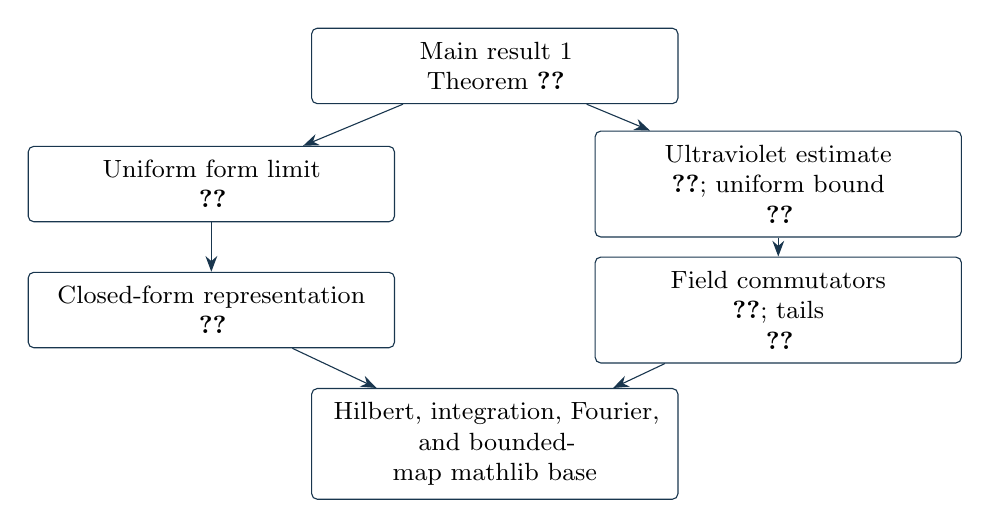
\begin{tikzpicture}[node distance=7mm and 8mm,
 box/.style={draw=inkblue,rounded corners=2pt,align=center,text width=43mm,
 inner sep=5pt,font=\small},arr/.style={-{Stealth[length=2mm]},draw=inkblue}]
\node[box] (root) at (0,0) {Main result 1\\Theorem~\ref{main:form-H}};
\node[box] (limit) at (-3.6,-1.5) {Uniform form limit\\\ref{basic:uniform-form-limit}};
\node[box] (uv) at (3.6,-1.5) {Ultraviolet estimate\\\ref{main:uv-form}; uniform bound\\\ref{main:uniform-form-bound}};
\node[box] (rep) at (-3.6,-3.1) {Closed-form representation\\\ref{basic:form-representation}};
\node[box] (field) at (3.6,-3.1) {Field commutators\\\ref{main:commutators}; tails\\\ref{model:frohlich-estimates}};
\node[box] (base) at (0,-4.8) {Hilbert, integration, Fourier,\\and bounded-map mathlib base};
\draw[arr] (root)--(limit);\draw[arr] (root)--(uv);
\draw[arr] (limit)--(rep);\draw[arr] (uv)--(field);
\draw[arr] (rep)--(base);\draw[arr] (field)--(base);
\end{tikzpicture}
\end{center}
The uniform form limit is taken on the already constructed complete
carrier $Q$. The representation theorem gives its full embedded energy
space, so the first target does not presuppose the interacting operator
domain formula.

\subsection{Exact domain by transport of mixed forms}
\begin{center}
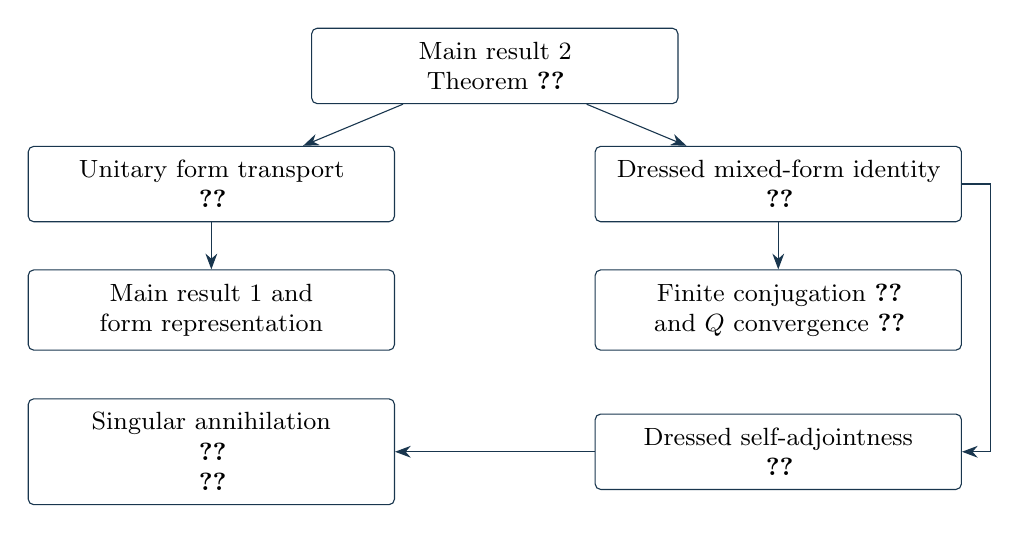
\begin{tikzpicture}[node distance=7mm and 8mm,
 box/.style={draw=inkblue,rounded corners=2pt,align=center,text width=43mm,
 inner sep=5pt,font=\small},arr/.style={-{Stealth[length=2mm]},draw=inkblue}]
\node[box] (root) at (0,0) {Main result 2\\Theorem~\ref{main:domain}};
\node[box] (transport) at (-3.6,-1.5) {Unitary form transport\\\ref{basic:unitary-form-transport}};
\node[box] (mixed) at (3.6,-1.5) {Dressed mixed-form identity\\\ref{main:dressed-form}};
\node[box] (construct) at (-3.6,-3.1) {Main result 1 and\\form representation};
\node[box] (finite) at (3.6,-3.1) {Finite conjugation \ref{main:conjugation}\\and $Q$ convergence \ref{main:gross-form}};
\node[box] (small) at (3.6,-4.9) {Dressed self-adjointness\\\ref{main:dressed-small}};
\node[box] (annih) at (-3.6,-4.9) {Singular annihilation\\\ref{main:singular-annihilation-limit}\\\ref{main:derivative-annihilation}};
\draw[arr] (root)--(transport);\draw[arr] (root)--(mixed);
\draw[arr] (transport)--(construct);\draw[arr] (mixed)--(finite);
\draw[arr] (mixed.east)--(6.3,-1.5)--(6.3,-4.9)--(small.east);
\draw[arr] (small)--(annih);
\end{tikzpicture}
\end{center}
The limiting identity holds on $Q\times Q$. The two inclusions in the
operator domain follow by writing down representing Hilbert vectors.
This avoids subtracting unbounded operators on unmatched domains and
avoids an unnecessary norm-resolvent branch.

\needspace{25\baselineskip}\subsection{Sharp regularity: two separate branches}
\begin{center}
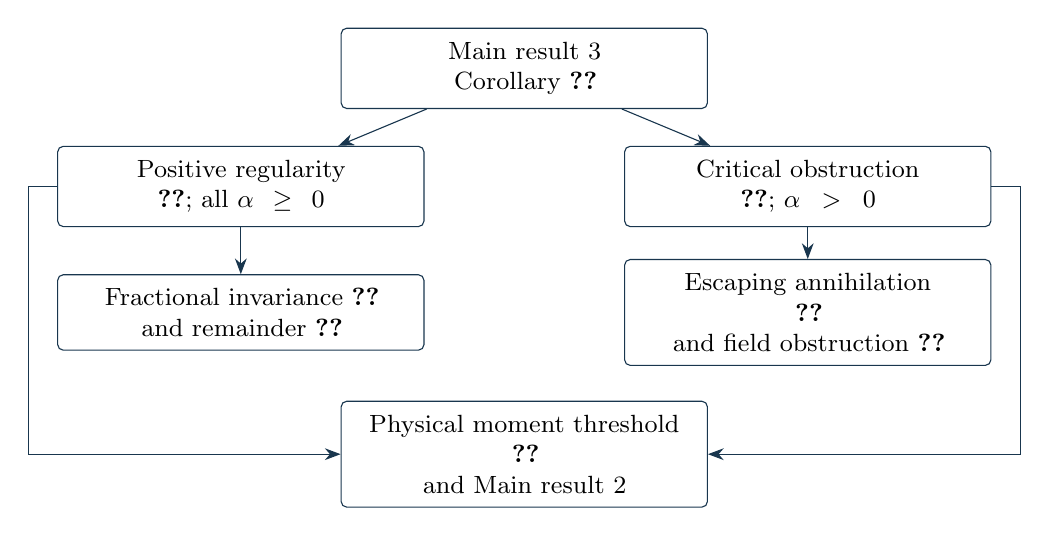
\begin{tikzpicture}[node distance=7mm and 8mm,
 box/.style={draw=inkblue,rounded corners=2pt,align=center,text width=43mm,
 inner sep=5pt,font=\small},arr/.style={-{Stealth[length=2mm]},draw=inkblue}]
\node[box] (root) at (0,0) {Main result 3\\Corollary~\ref{reg:main-corollary}};
\node[box] (pos) at (-3.6,-1.5) {Positive regularity\\\ref{reg:positive}; all $\alpha\geq0$};
\node[box] (neg) at (3.6,-1.5) {Critical obstruction\\\ref{reg:negative}; $\alpha>0$};
\node[box] (inv) at (-3.6,-3.1) {Fractional invariance \ref{reg:invariance}\\and remainder \ref{reg:remainder}};
\node[box] (escape) at (3.6,-3.1) {Escaping annihilation\\\ref{reg:annihilation_escape}\\and field obstruction \ref{reg:singular_field}};
\node[box] (moment) at (0,-4.9) {Physical moment threshold\\\ref{model:moment-threshold}\\and Main result 2};
\draw[arr] (root)--(pos);\draw[arr] (root)--(neg);
\draw[arr] (pos)--(inv);\draw[arr] (neg)--(escape);
\draw[arr] (pos.west)--(-6.3,-1.5)--(-6.3,-4.9)--(moment.west);
\draw[arr] (neg.east)--(6.3,-1.5)--(6.3,-4.9)--(moment.east);
\end{tikzpicture}
\end{center}
The negative branch normalizes coefficient norms only after proving they
diverge at positive coupling. The zero-coupling branch is settled
separately by $H_{\alpha=0}=H_0$. Momentum powers are explicit Fourier
multipliers throughout; no general unbounded spectral theorem is a leaf.

\paragraph{Independent parts.}
The form-representation lemmas, the concrete Fock construction, and the
three-dimensional coefficient estimates can be developed separately after
their indicated Hilbert and measure prerequisites. The Gross argument
joins these branches. The fractional regularity branch then uses the
exact-domain result, but is not needed to construct that domain.

\subsection{Execution contract for the later formalization}
\label{sec:execution-contract}
The three target environments are frozen specifications. Revision 10
changes no target statement and introduces no additional main theorem.
A supporting result is complete only after its statement, explicit
domain data, and proof have been formalized; a target is never an
assumption used to discharge its own prerequisites. The manuscript is
the authoritative mathematical text. Companion work packets are
extractions for navigation, not independent alternative proofs.

Work in the topological order of the direct dependency register.
Independent branches can be developed separately, but must share the
same carriers and interfaces from Section~\ref{sec:translation-design}.
Before starting a node, settle its listed prerequisites. When a proof
needs an additional local algebraic, measurable, or norm adapter,
prove it from mathlib and the already completed nodes; record any new
substantive dependency explicitly. Do not replace a missing proof by
an axiom, an external textbook citation, or an assumption of the
conclusion. Noncomputable choices are allowed when their existence
has been proved.

The mathematical argument is prescribed, not a research task for the
formalizer. The supporting lemmas in Section~\ref{sec:translation-bridges}
close the representative, graph-limit, differentiability, and finite
combinatorial interfaces that would otherwise invite new mathematics.
Routine expansion of definitions, type transport, algebraic rewrites,
and application of these proved statements are implementation work.
A new estimate, new compactness argument, new domain inclusion, or a
new analytic limiting theorem is not such routine work. If any such
obligation is found necessary despite this specification, record its
exact statement and the failed call site; do not silently invent a
replacement proof in Lean or mark that unit complete. The specification
must first be repaired mathematically. This boundary is a safeguard,
not a proof that elaboration will reveal no further issue.


For each accepted node, check the carrier, quantifiers, exceptional
parameter cases, domain equalities, representative independence,
measurability, integrability, and convergence topology. In particular,
operator equality includes equality of domains; convergence on a
core must be extended in the named graph norm; a cofinal sequence
limit needs the stated uniform tail control before it becomes a
limit over all cutoffs. Finally, each endpoint must prove the frozen
target on the physical space $\mathcal H$, not merely on an unspecified
isomorphic Hilbert space.

The machine-readable graph keeps all declared direct edges. A
transitive reduction is supplied only as a visualization, not as a
replacement for a lemma's direct mathematical contract. Shared
prerequisites are proved once and reused by all rooted views.

% ===== END PART: 02_structure =====

% ===== BEGIN PART: 03_carriers =====
\section{Fixed carriers, conventions, and domains}
\label{sec:translation-design}

The purpose of this section is to settle representation choices before
formalization. The choices below are part of the mathematical design,
not additional axioms. Every asserted adapter is proved in a named unit
of the manuscript. The three targets remain the conclusions to prove.
Each lemma below gives its actual proof where it is used in the
mathematical development. The dependency lines refer to earlier
proved lemmas or to the exact mathlib entries in the reference
catalogue. There is no separate proof-packet appendix.

\subsection{One carrier for each mathematical role}

\paragraph{Euclidean variables and measures.}
Use \nolinkurl{EuclideanSpace} over $\mathbb R$ on
$\operatorname{Fin}3$ for each copy of physical three-space. Position,
electron momentum, and phonon momentum have the same underlying type,
but the notation $x,q,k$ fixes their different roles. All three use
their Euclidean Borel Lebesgue measure. For finite phonon coordinates
use $X_n=(\operatorname{Fin}n\to\mathbb R^3)$ and the finite product
measure, not an unspecified iterated product. The permutation and
distinguished-coordinate maps, their directions, inverses, and measure
preservation are fixed in Lemma~\ref{fock:coordinate-model}.
The scalar vacuum remains $\mathcal F_0=\mathbb C$; its unitary
adapter to the empty-product $L^2$ space must be inserted explicitly.
It is not a definitional identification.

\paragraph{Hilbert-valued functions and sums.}
Use the existing Bochner \nolinkurl{MeasureTheory.Lp} carrier with
exponent $2$ for every $L^2$ space. Use the dependent \nolinkurl{lp}
carrier with exponent $2$ for the countable particle sum. A symmetric
sector is the common fixed closed complex subspace of its ambient
$L^2$ under the finitely many permutation isometries. It receives
the closed-subspace Hilbert structure after closedness is proved.
The two models $L^2(dx;\mathcal F)$ and
$\bigoplus_n L^2(dx;\mathcal F_n)$ are connected by the proved
electron--Fock unitary. Transport an operator together with its domain
through this unitary. Do not silently equate its two ambient carriers.

\paragraph{Weighted domains.}
For a finite measurable $w\geq1$ and a closed subspace $S$ stable
under the reciprocal and truncation multipliers specified in
Lemma~\ref{basic:weighted-carrier}, use the notation
$\mathsf W(w;S)$ for a named copy of the already complete Hilbert
space $S$. Its embedding in the ambient space is
\[
 J_w f=w^{-1}f,\qquad
 \operatorname{ran}J_w=D_w(S),\qquad
 \|J_wf\|_{D_w}=\|wJ_wf\|=\|f\|_S.
\]
The physical vector represented by $f$ in this carrier is $J_wf$.
The inverse coordinate of $u\in D_w(S)$ is $wu$.
This settles both the carrier and the norm. In particular, the
ambient subtype norm on $D_w(S)$ is not the weighted norm.
For number graph spaces $D((N+1)^r)$ use $w_n=(1+n)^r$ and the same
reciprocal construction in the dependent sum. For free form and
free operator graph spaces use the weights in
Lemma~\ref{basic:free}; where an equivalent weight is convenient,
retain the proved two comparison constants and the same ambient
embedding. Symmetric sectors are invariant under the weights used
here because those weights are unchanged by phonon permutations.
The abstract carrier lemma explicitly requires the invariance
hypotheses; closedness alone does not imply them.

An ambient linear map $T$ preserves a weighted domain with a proved
bound precisely when it has the bounded lift
$\widetilde T f=vT(w^{-1}f)$ with
$J_v\widetilde T=TJ_w$. The two directions, uniqueness, compositions,
and inverses of these lifts are proved in the same lemma. Use this
single construction for Weyl preservation of number and form domains.

\paragraph{General graph spaces and energy spaces.}
For a closed operator $A:E\supset D(A)\to F$, represent its graph
as a closed complex subspace of \nolinkurl{WithLp} with exponent
$2$ on $E\times F$. Its inner product is the sum of the two
coordinate inner products. The graph coordinate map
$u\mapsto(u,Au)$ is an isometry for
$(\|u\|^2+\|Au\|^2)^{1/2}$. A raw product type has a different
default norm. Lemma~\ref{basic:graph-integration} supplies the
closed graph and Bochner integration statements in the correct norm.

For a positive shifted form $q_c$ on an already constructed carrier
$Q$, keep two named copies if both inner products are needed:
the original reference Hilbert space $Q$, and $Q_c$ with inner
product $q_c$. In Theorem~\ref{basic:form-representation}, the
constants $\delta,M>0$ prove
$\delta\|u\|_Q^2\leq q_c(u,u)\leq M\|u\|_Q^2$.
These inequalities prove completeness of $Q_c$ and continuity of
the identity maps between the two copies. They must precede any
Hilbert-space argument in $Q_c$. The separate energy carrier
$E_c=D(H)$ has inner product $\langle u,(H+c)v\rangle$;
the theorem proves its completion isometry to $Q_c$ and compatibility
with the ambient embedding. This is the meaning of the form-domain
conclusion, without importing unbounded spectral calculus.

\subsection{Partial operators, forms, and equality}

\paragraph{Operator data.}
Use \nolinkurl{LinearPMap} for a complex linear map with an explicit
linear domain. Denseness, closedness, symmetry, and self-adjointness
are properties of that map with its domain. The bridge in
Lemma~\ref{basic:partial-operator-bridge} relates the manuscript's
adjoint witness condition to the documented partial-map adjoint and
closure interfaces. Self-adjointness here includes a dense domain
and equality with that adjoint. It is not the bounded-algebra
self-adjoint predicate applied to an arbitrary partial map.

For a sequential product $AB$, the domain is
\[
 \{u\in D(B):Bu\in D(A)\},\qquad (AB)u=A(Bu).
\]
Every evaluation in a proof therefore has two membership witnesses.
An equality $A=B$ is proved by both domain inclusions and action
equality on that domain. An inclusion $A\subset B$ carries the
corresponding one-sided witnesses. A maximal product multiplier is
defined directly from the product function; it is compared with a
sequential product only after a separate domain proof. This distinction
is used explicitly for vacuum sectors and mixed number--momentum
weights.

If a bounded injective self-adjoint map $R$ is inverted on its range,
define the resulting operator on the subspace $\operatorname{ran}R$:
$S(Rf)=f$. Injectivity gives uniqueness of the witness $f$.
Lemma~\ref{basic:inverse-operator} proves the domain, both inverse
identities, both adjoint inclusions, and the graph-coordinate core
transport. No value of $S$ is needed off its domain.

\paragraph{Sesquilinear orientation.}
Every inner product is conjugate-linear in the first variable.
A bounded form is bundled as a continuous conjugate-linear map
in the first variable with values in the continuous linear dual
in the second variable. The listed declaration
\nolinkurl{InnerProductSpace.continuousLinearMapOfBilin} gives
$\langle Tu,v\rangle=b(u,v)$. For a Hermitian form the conjugation
calculation in Lemma~\ref{basic:polarization} gives
$b(u,v)=\langle u,Tv\rangle$. Perform that calculation before
using the latter identity. Real inequalities for diagonal complex
forms mean inequalities for their real parts, with zero imaginary
part proved by Hermitian symmetry.

Annihilation is conjugate-linear and creation linear in the test
coefficient. The Weyl convention and the sign
$U_{\alpha,K}=W(-B_{\alpha,K})$ remain fixed throughout.
Coherent vectors are unnormalized. Their tensor normalization,
factorial coefficients, and all required derivatives are proved in
Lemma~\ref{fock:coherent-jets}. The subsequent Weyl calculations
use those exact identities.

\subsection{Representative, approximation, and limit rules}

\paragraph{Representatives.}
Before defining an $L^2$ element, provide almost-everywhere strong
measurability and the integral of its squared norm. Before applying
an operation to its equivalence class, prove independence from
representatives. A finite or countable family of almost-everywhere
identities may share a null exceptional set by taking the corresponding
union. An uncountable family may not. Operator equalities for all
vectors are equalities of classes; they do not assert one pointwise
null set that works for every vector simultaneously.

For graph-valued or Fock-valued reconstruction, choose the strongly
measurable limit supplied by the explicit approximation in the
relevant proof. Its image in the ambient space equals the desired
class almost everywhere. A pointwise expression for coordinates is
not by itself a proof of strong measurability in a stronger graph norm.
All integrals in a possibly divergent nonnegative estimate take
values in $[0,+\infty]$. Convert to a real integral only after
finiteness is established.

\paragraph{Density and witnesses.}
Whenever a dense set is used to approximate $u$, choose the $n$th
approximant with error below $(n+1)^{-1}$ in the named norm.
The existence proof for each approximant and the specified error
bound justify the resulting sequence. No computable choice is
required, but the existence proposition must be proved. For two
successive approximations, allocate half the desired error to each
and apply the triangle inequality. The weighted smooth-product
density proof uses this pattern with the actual number and momentum
weights. Applying a closed operator to a limit requires convergence
of both the input and its image in the stated ambient Hilbert spaces.

\paragraph{Cutoffs and estimates.}
For finite ultraviolet expressions use the exact cutoff convention
of the corresponding statement, including strict or non-strict
endpoints. Differences on a sphere are removed by a proved null-set
fact where necessary. For sequential approximation fix an increasing
sequence above the infrared cutoff, as specified in the local proof.
To conclude a limit over all real cutoffs, supply a tail estimate
valid for every sufficiently large cutoff; convergence along that
one sequence is insufficient. Lemma~\ref{model:cutoff-witness}
fixes positive witnesses for all the smallness and tail requirements,
including the explicit $K_0(\alpha)$. Thus the quantifier
``every $K\geq K_0(\alpha)$'' is carried by a single monotone bound.
The branch $\alpha=0$ is proved before any normalization by a
nonzero coefficient norm.
% ===== END PART: 03_carriers =====

% ===== BEGIN PART: 04_generic_foundations =====
\section{Foundational interfaces and explicit analytic constructions}
\label{sec:foundations}

\subsection{Conventions and the mathematical base}

All Hilbert spaces are complex, and $\langle u,v\rangle$ is conjugate-linear in
$u$ and linear in $v$. An unbounded operator includes its linear domain as part
of its data. An operator identity includes an equality of domains, unless it is
explicitly described as an identity on a common subspace. A form is a
sesquilinear form; ``quadratic form'' means its diagonal. All measurable
functions and all parity identities may be taken modulo null sets. Every
physical position or momentum variable lies in $\mathbb R^3$. Abstract
Hilbert-space and measure-space lemmas are stated only at the generality
needed to construct this fixed three-dimensional model.
Whenever a diagonal form value or $\langle u,Au\rangle$ is compared with a
real number, the expression is real by Hermitian symmetry; equivalently,
the inequality is an inequality between real parts. This convention does
not identify complex numbers with an ordered field. The Hilbert-valued
$L^2$ spaces below are Bochner spaces of almost-everywhere strongly
measurable representatives, modulo almost-everywhere equality. The measure
spaces in the weighted-model statements are $\sigma$-finite; all uses here
are Lebesgue spaces, counting spaces, and their finite or countable
disjoint-union products. A measurable scalar multiplier is finite almost
everywhere, and may be assigned zero on its exceptional null set. Products,
domains, and equalities of $L^2$ classes are independent of the chosen
representatives because pointwise multiplication preserves
almost-everywhere equality.

The imported mathematical base consists of complete Hilbert spaces, continuous
linear maps and their adjoints, the Hilbert-space Riesz representation theorem,
Lebesgue and Bochner integration, Tonelli, monotone and dominated convergence,
the Cauchy--Schwarz and H\"older inequalities, countable $\ell^2$ sums, and the
Hilbert-valued $L^2$ Fourier isometry. Precise source locations and the limits of
the reference checks appear in Section~\ref{sec:mathlib-audit}. The results below
are \emph{proved project lemmas}, even when they are
familiar textbook mathematics. In particular, closed-form representation,
Kato--Rellich, unbounded spectral calculus, and Fock-space theory are not
being silently imported. The later field-operator calculus is developed
from explicit Weyl operators; no theorem about Hamiltonian time evolution
is required.

\begin{lemma}[Hermitian form bounds from diagonal bounds]
\label{basic:polarization}
\proofid{basic:polarization}
\par\smallskip{\normalfont\small\noindent\textbf{Direct prerequisites.} Mathlib: \hyperref[base:M010]{M010}, \hyperref[base:M011]{M011}, \hyperref[base:M012]{M012}, \hyperref[base:M013]{M013}, \hyperref[base:M118]{M118}, \hyperref[base:M119]{M119}, \hyperref[base:M120]{M120}, \hyperref[base:M121]{M121}.}\par\smallskip

Let $b$ be a Hermitian sesquilinear form on an inner-product space $E$ and let
$C\geq0$. If $|b(u,u)|\leq C\|u\|^2$ for every $u$, then
$|b(u,v)|\leq C\|u\|\|v\|$ for all $u,v$. If $E$ is complete, there is a
unique bounded self-adjoint operator $B$ with $b(u,v)=\langle u,Bv\rangle$,
and $\|B\|\leq C$.
\end{lemma}
\begin{proof}
The case of a zero argument is immediate. Divide both arguments by their
norms. If their pairing is zero there is nothing to prove; otherwise put
$z=b(u,v)$ and multiply the second unit vector by
$\overline z/|z|$. This scalar has modulus one and, because the second
variable is linear, the new pairing is $|z|$, real and nonnegative. For these unit vectors, the polarization identity and
the parallelogram identity give
\[
4|b(u,v)|=b(u+v,u+v)-b(u-v,u-v)
 \leq C(\|u+v\|^2+\|u-v\|^2)=4C.
\]
Rescale. Riesz representation applied with the second argument fixed gives
$Bv$: the continuous conjugate-linear functional $u\mapsto b(u,v)$ has
the unique form $u\mapsto\langle u,Bv\rangle$. For $v,w\in E$ and
$\lambda,\mu\in\mathbb C$, sesquilinearity and uniqueness give
$B(\lambda v+\mu w)=\lambda Bv+\mu Bw$. If $Bv\ne0$, test
the bilinear bound with $u=Bv/\|Bv\|$ to get
$\|Bv\|\leq C\|v\|$; the zero case is immediate.
Finally
$\langle u,Bv\rangle=b(u,v)=\overline{b(v,u)}=\langle Bu,v\rangle$,
which is exactly the bounded-adjoint characterization of $B^*=B$.

For the exact mathlib Riesz interface, first view the bounded form as a
continuous conjugate-linear map in its first variable with values in the
continuous linear dual in its second variable; the estimate above supplies
both continuity bounds. The declaration
\nolinkurl{InnerProductSpace.continuousLinearMapOfBilin} produces a map
$T$ with $\langle Tu,v\rangle=b(u,v)$. This orientation differs from
the displayed convention, but Hermitian symmetry gives
\[
 b(u,v)=\overline{b(v,u)}
       =\overline{\langle Tv,u\rangle}=\langle u,Tv\rangle.
\]
Thus the same $T$ is the required $B$, and the adjoint identity is proved
before its self-adjointness is used. This explicitly reconciles the
library convention with the form convention.
\end{proof}

\begin{lemma}[Dense determination and varying-argument limits of bounded forms]
\label{basic:mixed-form-limits}
\proofid{basic:mixed-form-limits}
\par\smallskip{\normalfont\small\noindent\textbf{Direct prerequisites.} Elementary Hilbert-space norm, linearity, and limit properties only.}\par\smallskip

Let $E$ be a complex Hilbert space. A bounded sesquilinear form
$b$ is conjugate-linear in its first argument and linear in its second;
its norm is the least $C\geq0$ such that
$|b(u,v)|\leq C\|u\|\|v\|$. The following two statements hold.

If two bounded forms $b,c$ agree on $\mathcal D\times\mathcal D$,
where $\mathcal D$ is a dense linear subspace of $E$, they agree
on all of $E\times E$.

Suppose $b_\lambda,b$ are bounded forms with
$\|b_\lambda-b\|\to0$ as $\lambda\to\infty$, and
$u_\lambda\to u$, $v_\lambda\to v$ in $E$. Then
$b_\lambda(u_\lambda,v_\lambda)\to b(u,v)$. More precisely,
\begin{align*}
 |b_\lambda(u_\lambda,v_\lambda)-b(u,v)|
 &\leq\|b_\lambda-b\|\|u_\lambda\|\|v_\lambda\|\\
 &\quad+\|b\|\|u_\lambda-u\|\|v_\lambda\|
       +\|b\|\|u\|\|v_\lambda-v\|.
\end{align*}
The parameter may be a sequence or a positive real cutoff. In
particular the assertion is not restricted to integer cutoffs.
\end{lemma}
\begin{proof}
For the first assertion, choose $u_n,v_n\in\mathcal D$ with
$\|u_n-u\|,\|v_n-v\|<(n+1)^{-1}$, using density separately
for the two vectors. Set $d=b-c$. By sesquilinearity,
\[
 d(u,v)-d(u_n,v_n)=d(u-u_n,v)+d(u_n,v-v_n).
\]
Taking absolute values bounds the right side by
$\|d\|((n+1)^{-1}\|v\|+(\|u\|+1)(n+1)^{-1})$.
It tends to zero, whereas $d(u_n,v_n)=0$. Thus $d(u,v)=0$.
This proves the equality for each ordered pair, not merely on
diagonal quadratic values.

For the second assertion, add and subtract
$b(u_\lambda,v_\lambda)$ and $b(u,v_\lambda)$. The resulting
three terms are
\[
 (b_\lambda-b)(u_\lambda,v_\lambda),\qquad
 b(u_\lambda-u,v_\lambda),\qquad b(u,v_\lambda-v).
\]
Apply the defining bound to each term and then the scalar triangle
inequality. Convergence of the two vector families implies that,
after one threshold, $\|u_\lambda\|\leq\|u\|+1$ and
$\|v_\lambda\|\leq\|v\|+1$. Replace these two factors by
these fixed finite bounds. Each of the other three factors tends
to zero. For a tolerance $\varepsilon>0$, choose a threshold
making each term at most $\varepsilon/3$, with denominators
increased by $1$ if a fixed coefficient is zero. The maximum of
the three thresholds proves the claimed limit over the original
parameter set.
\end{proof}


\begin{lemma}[A positive bounded operator has a bounded inverse]
\label{basic:coercive-bounded}
\proofid{basic:coercive-bounded}
\par\smallskip{\normalfont\small\noindent\textbf{Direct prerequisites.} Mathlib: \hyperref[base:M010]{M010}, \hyperref[base:M067]{M067}, \hyperref[base:M118]{M118}, \hyperref[base:M119]{M119}, \hyperref[base:M120]{M120}.}\par\smallskip

If $B=B^*$ is bounded on a Hilbert space $E$ and
$\langle u,Bu\rangle\geq c\|u\|^2$ for some $c>0$, then $B$ is bijective
and $\|B^{-1}\|\leq c^{-1}$.
\end{lemma}
\begin{proof}
Cauchy--Schwarz gives
$c\|u\|^2\leq |\langle u,Bu\rangle|\leq\|u\|\|Bu\|$.
For $u\ne0$ divide by $\|u\|$; for $u=0$ the resulting bound
$c\|u\|\leq\|Bu\|$ holds directly. It implies injectivity and,
by applying it to $u_n-u_m$, makes $u_n$ Cauchy whenever $Bu_n$
converges. Completeness gives a limit $u$ and continuity gives
$Bu=\lim_nBu_n$. Thus the range is closed. If $y$ is orthogonal to
the range, then
$0=\langle Bx,y\rangle=\langle x,B^*y\rangle$ for every $x$;
taking $x=B^*y$ gives $B^*y=0$. The converse is the same identity.
Since $B^*=B$ is injective, the range has zero orthogonal complement.
Its closure is therefore the whole Hilbert space, and its closedness
makes $B$ surjective.

Define $B^{-1}f$ to be the unique vector $u$ with $Bu=f$.
Linearity follows by applying $B$ to a proposed linear combination and
using injectivity. The lower bound, applied to this vector, gives
$\|B^{-1}f\|\leq c^{-1}\|f\|$, so this is a bounded linear map
and its operator norm is at most $c^{-1}$. The two inverse identities
hold on every vector; they are not only identities on a dense range.
\end{proof}


\begin{lemma}[Closed graphs and integration in an operator domain]
\label{basic:graph-integration}
\proofid{basic:graph-integration}
\par\smallskip{\normalfont\small\noindent\textbf{Direct prerequisites.} Mathlib: \hyperref[base:M050]{M050}, \hyperref[base:M053]{M053}, \hyperref[base:M054]{M054}, \hyperref[base:M058]{M058}, \hyperref[base:M059]{M059}, \hyperref[base:M087]{M087}, \hyperref[base:M088]{M088}, \hyperref[base:M089]{M089}, \hyperref[base:M090]{M090}.}\par\smallskip

Let $A:D(A)\subset E\to F$ be a closed linear operator between complex
Hilbert spaces. Its domain, with inner product
\[
 \langle u,v\rangle_A=\langle u,v\rangle_E+\langle Au,Av\rangle_F,
 \qquad \|u\|_A^2=\|u\|^2+\|Au\|^2,
\]
is a Hilbert space. If $f:S\to D(A)$, both the ambient $E$-valued
map $f$ and the $F$-valued map $Af$ are almost-everywhere strongly measurable, and the
nonnegative function $s\mapsto\|f(s)\|+\|Af(s)\|$ is integrable,
equivalently its nonnegative extended integral is finite,
\[
 \int_S^{\!+}\bigl(\|f(s)\|+\|Af(s)\|\bigr)\,d\mu(s)<\infty,
\]
then the ambient Bochner integral belongs to $D(A)$ and
\[
 A\int_S f(s)\,d\mu(s)=\int_S Af(s)\,d\mu(s).
\]
The same assertion applies to integrals over finite or infinite real
intervals, provided the displayed integrability condition is checked.
\end{lemma}
\begin{proof}
Equip the product vector space with the Hilbert norm
$\|(x,y)\|_2=(\|x\|^2+\|y\|^2)^{1/2}$ and the sum inner product.
In Lean this is \texttt{WithLp 2} applied to $E\times F$, with
\nolinkurl{WithLp.instProdInnerProductSpace}; it must not be replaced
by the raw product type's default maximum norm when asserting an
isometry. The inequalities
\[
 \max(\|x\|,\|y\|)\leq\|(x,y)\|_2
 \leq\sqrt2\max(\|x\|,\|y\|)
\]
show that the Hilbert product and ordinary product have the same
topology, so the assumed closedness of the graph is unchanged.
The map $u\mapsto(u,Au)$ is an isometry from the stated graph norm
onto this closed linear graph. Its inverse is the first coordinate
restricted to the graph, whose graph membership ensures that the
second coordinate is its image under $A$. A closed subspace of a
Hilbert space is complete, so the graph norm is complete. The two coordinate maps from this graph space
are bounded, with norms at most one. To check almost-everywhere strong
measurability in the graph norm, start with the corresponding pair $(f,Af)$ in
this Hilbert product. Approximate this pair almost everywhere by simple
functions, then project those simple functions orthogonally onto the
closed graph. The projected simple functions still converge almost
everywhere, since the graph projection fixes $(f,Af)$. Pulling them
back by the graph isometry gives graph-valued simple approximations.
The graph norm is at most $\|f\|+\|Af\|$, so the graph-valued function
is Bochner integrable. Apply the two bounded coordinate maps to its
integral. The first gives the ambient integral of $f$, and the second
gives the integral of $Af$. Since the pair is in the graph, the asserted
domain membership and identity follow.
\end{proof}


\begin{lemma}[Extending identities into a closed operator domain]
\label{basic:closed-graph-extension}
\proofid{basic:closed-graph-extension}
\par\smallskip{\normalfont\small\noindent\textbf{Direct prerequisites.} Project: \ref{basic:graph-integration}.}\par\smallskip

Let $X,E,F,G$ be Hilbert spaces, $J:X\to E$, $T:E\to F$,
and $L:X\to G$ bounded linear maps, and $C\subset X$ a dense
linear subspace. Let $A:D(A)\subset F\to G$ be a closed linear
operator. Suppose that, for every $c\in C$,
\[
 TJc\in D(A),\qquad ATJc=Lc.
\]
Then, for every $u\in X$, $TJu\in D(A)$ and $ATJu=Lu$.
In particular the map $u\mapsto TJu$ into the graph Hilbert space
of $A$ is bounded, with
\[
 \|TJu\|_A^2=\|TJu\|_F^2+\|Lu\|_G^2
 \leq\bigl(\|T\|^2\|J\|^2+\|L\|^2\bigr)\|u\|_X^2.
\]
Also, if two bounded sesquilinear forms on $X$ agree on $C\times C$,
they agree on $X\times X$.
\end{lemma}
\begin{proof}
For fixed $u\in X$, density supplies $c_n\in C$ with
$\|c_n-u\|_X<1/(n+1)$. Boundedness gives
$TJc_n\to TJu$ in $F$ and $Lc_n\to Lu$ in $G$.
The pairs $(TJc_n,ATJc_n)=(TJc_n,Lc_n)$ lie in the graph of
$A$ and converge to $(TJu,Lu)$. Closedness of that graph gives
both the claimed domain membership and the value of $A$.
The displayed graph estimate then follows from the two bounded-map
estimates. Lemma~\ref{basic:graph-integration} supplies the graph
Hilbert-space structure. This argument does not apply $A$ to a limit
before proving that the limit belongs to its domain.

For the form assertion let $d$ be the difference of the two forms.
The sum $M$ of their nonnegative bounds satisfies
$|d(x,y)|\leq M\|x\|_X\|y\|_X$. Choose $c_n\to u$ and
$e_n\to v$ in $C$. The sequence $\|e_n\|_X$ is bounded, and
\[
 |d(u,v)-d(c_n,e_n)|
 \leq M\|u-c_n\|_X\|e_n\|_X
       +M\|u\|_X\|v-e_n\|_X\longrightarrow0.
\]
Since $d(c_n,e_n)=0$, the limit is $d(u,v)=0$.
In applications, $X$ carries the \emph{specified} graph or form
norm, and density of $C$ and boundedness of $J,T,L$ must be proved
in those norms. Density in the ambient norm alone is insufficient.
\end{proof}


\begin{lemma}[Uniform strong limits obtained from a dense subspace]
\label{basic:dense-strong-limit}
\proofid{basic:dense-strong-limit}
\par\smallskip{\normalfont\small\noindent\textbf{Direct prerequisites.} Elementary Hilbert-space norm, linearity, and limit properties only.}\par\smallskip

Let $E,F$ be Hilbert spaces and $D\subset E$ a dense linear subspace.
Let the parameter $t$ range over a metric space, for example a space of Weyl coefficients.
Suppose $T_n(t):E\to F$ are bounded linear maps. On every compact
parameter set $I$, assume
\[
 \sup_{n,t\in I}\|T_n(t)\|\leq M_I<\infty,
\]
and assume that $T_n(t)v$ is uniformly Cauchy for $t\in I$ for each
$v\in D$. Then $T_n(t)u$ converges uniformly on $I$ for every $u\in E$.
The pointwise limits $T(t)$ are bounded linear maps with
$\|T(t)\|\leq M_I$ for $t\in I$. If $t\mapsto T_n(t)u$ is continuous
for every $n,u$, the limiting orbit is continuous. In addition, if
$S_n\to S$ and $T_n\to T$ strongly at fixed parameters and
$\sup_n\|T_n\|<\infty$, then $T_nS_n\to TS$ strongly.
\end{lemma}
\begin{proof}
For $u\in E$ choose $v\in D$. Uniformly for $t\in I$,
\[
 \|(T_n(t)-T_m(t))u\|
 \leq2M_I\|u-v\|+\|(T_n(t)-T_m(t))v\|.
\]
First make the first term small by density and then the second by the
assumed uniform Cauchy property. Completeness of $F$ gives pointwise
limits; passing $m\to\infty$ in the same estimate proves uniform
convergence. Linearity and the bound pass to the limit for each fixed
$t$. To check continuity at $t$, take any sequence $t_j\to t$.
The set $\{t\}\cup\{t_j:j\geq1\}$ is compact, so uniform
convergence there and continuity of the approximants imply
$T(t_j)u\to T(t)u$. Sequential continuity is continuity in a metric
space. Finally, for each $u$,
\[
 \|T_nS_nu-TSu\|
 \leq\|T_n\|\,\|S_nu-Su\|+\|(T_n-T)Su\|\longrightarrow0.
\]
This product statement is at fixed parameters; no unjustified uniform
convergence on the entire unit ball is asserted. In this last assertion
$S_n,S:G\to E$ and $T_n,T:E\to F$ are bounded linear maps between
fixed Hilbert spaces; strong convergence means convergence at every
fixed vector, and the displayed bound applies separately to each
$u\in G$. No boundedness assumption on the entire sequence $S_n$ is
needed for this estimate.
\end{proof}


\subsection{Unbounded operators and resolvents}

\begin{lemma}[Partial-operator, adjoint, and core interfaces]
\label{basic:partial-operator-bridge}
\proofid{basic:partial-operator-bridge}
\par\smallskip{\normalfont\small\noindent\textbf{Direct prerequisites.} Project: \ref{basic:graph-integration}. Mathlib: \hyperref[base:M032]{M032}, \hyperref[base:M033]{M033}, \hyperref[base:M035]{M035}, \hyperref[base:M036]{M036}, \hyperref[base:M037]{M037}, \hyperref[base:M038]{M038}, \hyperref[base:M039]{M039}, \hyperref[base:M040]{M040}, \hyperref[base:M132]{M132}, \hyperref[base:M133]{M133}.}\par\smallskip

Let $T:D(T)\subset E\to F$ be a densely defined linear operator between
complex Hilbert spaces. Bundle its domain as a complex linear subspace
and its action as a linear map on that subspace. Its adjoint defined by
\[
 D(T^\sharp)=\{y\in F:\exists h\in E\ \forall x\in D(T),
                     \ \langle Tx,y\rangle=\langle x,h\rangle\},
 \qquad T^\sharp y=h,
\]
is precisely \nolinkurl{LinearPMap.adjoint}, with equality of domains
and actions. If $T$ is closed and $C$ is a linear subspace of $D(T)$,
then $C$ is dense in $D(T)$ for
$\|x\|_T=(\|x\|^2+\|Tx\|^2)^{1/2}$ if and only if the bundled
operator satisfies \nolinkurl{LinearPMap.HasCore} for $C$.
\end{lemma}
\begin{proof}
\noindent\textbf{Explicit translation step.} The explicit API route for a representing vector $h$ is as follows.
Conjugate $\langle Tx,y\rangle=\langle x,h\rangle$ to obtain
$\langle h,x\rangle=\langle y,Tx\rangle$. M132 gives membership of $y$
in the adjoint domain. After the dense-domain hypothesis has been
supplied, M133 gives the value $T^*y=h$. These are two separate witnesses;
the graph arguments below identify the full domains as well.

For fixed $y$, two representing vectors $h_1,h_2$ have
$\langle x,h_1-h_2\rangle=0$ on the dense domain. By continuity this
holds for all $x\in E$; taking $x=h_1-h_2$ gives uniqueness.
The zero vector is represented by zero. If $y_j$ is represented by
$h_j$, then $\lambda y_1+\mu y_2$ is represented by
$\lambda h_1+\mu h_2$, since the inner product is linear in its
second variable. Thus the displayed set is a subspace and its
uniquely defined action is linear. It is an operator, not merely a
relation with possibly several output vectors.

The defining pairing says that $T$ and $T^\sharp$ are formal
adjoints. Apply \nolinkurl{LinearPMap.IsFormalAdjoint.le_adjoint}
with the proved dense domain of $T$ to obtain
$T^\sharp\subseteq T^\dagger$, where $T^\dagger$ is the library
adjoint. Conversely,
\nolinkurl{LinearPMap.adjoint_isFormalAdjoint} with the same dense-domain
proof gives
$\langle T^\dagger y,x\rangle=\langle y,Tx\rangle$ for
$y\in D(T^\dagger)$ and $x\in D(T)$. Conjugating this equality
puts $y$ in the displayed set, represented by $T^\dagger y$.
The uniqueness already proved identifies the actions. The two
inclusions therefore prove equality of partial operators. Density
is supplied before either adjoint theorem is used: the library's
total adjoint definition has a fallback value when its source domain
is not dense, and that branch has no role here.

For the core assertion, write $T_C$ for the restriction with domain
exactly $C$. Its graph lies in the closed graph of $T$, so its
ambient topological closure $G$ also lies in that graph. In
particular $(0,y)\in G$ forces $y=T0=0$. The first-coordinate
projection is consequently injective on the linear subspace $G$.
Define an operator on its first-coordinate image by assigning to
$x$ the unique $y$ with $(x,y)\in G$. Addition and scalar
multiplication in $G$ make this action linear and its graph is
exactly $G$. This proves $T_C$ closable directly from the definition
of \nolinkurl{LinearPMap.IsClosable}; it does not assume in advance
that the library's closure is the desired operator.
Now \nolinkurl{LinearPMap.IsClosable.graph_closure_eq_closure_graph}
identifies $G$ with the graph of $T_C$'s library closure. The
restriction has domain $C$ because $C\subseteq D(T)$.

The graph map $x\mapsto(x,Tx)$ is an onto linear isometry from the
graph-norm domain to $\operatorname{graph}T$ in the Hilbert product,
by Lemma~\ref{basic:graph-integration}. This product has the same
topology as the ordinary product used in
\nolinkurl{LinearPMap.IsClosed}. Its image of $C$ is
$\operatorname{graph}T_C$. Consequently graph-norm density is
exactly $G=\operatorname{graph}T$. Equality of graphs determines
domain and action, so it is exactly $T_C.\mathrm{closure}=T$.
Together with $C\subseteq D(T)$, these are precisely the two fields
of \nolinkurl{LinearPMap.HasCore}. This proves both directions.
\end{proof}


\begin{lemma}[The range criterion for self-adjointness]
\label{basic:selfadjoint-criterion}
\proofid{basic:selfadjoint-criterion}
\par\smallskip{\normalfont\small\noindent\textbf{Direct prerequisites.} Project: \ref{basic:partial-operator-bridge}. Mathlib: \hyperref[base:M037]{M037}, \hyperref[base:M041]{M041}, \hyperref[base:M042]{M042}, \hyperref[base:M043]{M043}, \hyperref[base:M067]{M067}.}\par\smallskip

Let $T$ be densely defined and symmetric. If both $T-i\lambda$ and
$T+i\lambda$ are onto for some $\lambda>0$, then $T=T^*$, including
equality of domains. A self-adjoint $T$ is closed, and for every nonreal
$z$, $(T-z)^{-1}$ exists with norm at most $|\operatorname{Im}z|^{-1}$.
\end{lemma}
\begin{proof}
We construct the adjoint with its domain, rather than starting from
a total map on $\mathcal H$. Put
\[
 D(T^*)=\{y\in\mathcal H:\exists h\in\mathcal H\ \forall x\in D(T),
                \ \langle Tx,y\rangle=\langle x,h\rangle\}.
\]
If $h_1,h_2$ both work, then $h_1-h_2$ is orthogonal to the dense
subspace $D(T)$ and is zero. Define $T^*y$ to be this unique $h$.
Sesquilinearity in the displayed second arguments proves that the
witness for $\lambda y_1+\mu y_2$ is
$\lambda T^*y_1+\mu T^*y_2$; hence $D(T^*)$ is a linear subspace
and $T^*$ is linear on it. If $y_n\to y$ and $T^*y_n\to h$, pass to
the limit in the identity for each fixed $x\in D(T)$, using continuity
of the two inner products. The resulting identity says precisely
$y\in D(T^*)$ and $T^*y=h$, so its graph is closed. Symmetry of
$T$ says that every $y\in D(T)$ belongs to this adjoint domain and
$T^*y=Ty$.

For later use, for each $z\in\mathbb C$ the definition directly gives
\[
 D((T-z)^*)=D(T^*),\qquad (T-z)^*=T^*-\overline z,
 \qquad
 \operatorname{ran}(T-z)^\perp=\ker(T^*-\overline z).
\]
Indeed $\langle(T-z)x,y\rangle
=\langle Tx,y\rangle-\overline z\langle x,y\rangle$;
adding or subtracting $\overline z\,y$ from the representing vector
proves the domain equality, and setting that vector equal to zero
proves the orthogonal-complement formula. These assertions do not
assume beforehand that $T$ is closed or self-adjoint.

For $y\in D(T^*)$, choose $x\in D(T)$ with
$(T-i\lambda)x=(T^*-i\lambda)y$. The difference $y-x$ belongs to
$\ker(T^*-i\lambda)$, which is the orthogonal complement of
$\operatorname{ran}(T+i\lambda)$ and hence is zero. This proves equality
of domains and actions. Since the adjoint graph is closed, $T$ is now closed. For nonreal $z$, symmetry gives
\[
 \|(T-z)u\|\,\|u\|\geq
 |\operatorname{Im}\langle u,(T-z)u\rangle|
 =|\operatorname{Im}z|\,\|u\|^2.
\]
To see that the range is closed, let $(T-z)u_n\to f$.
The estimate makes $u_n$ Cauchy, hence $u_n\to u$; then
$Tu_n=(T-z)u_n+zu_n\to f+zu$. Closedness of $T$ gives
$u\in D(T)$ and $(T-z)u=f$.
Its orthogonal complement is $\ker(T-\overline z)$, which is zero by
the same estimate. Thus the range is the whole Hilbert space and the
inverse has the asserted bound.
\end{proof}

\begin{lemma}[Adjoint reversal and maximality of a self-adjoint restriction]
\label{basic:selfadjoint-inclusion}
\proofid{basic:selfadjoint-inclusion}
\par\smallskip{\normalfont\small\noindent\textbf{Direct prerequisites.} Project: \ref{basic:partial-operator-bridge}. Mathlib: \hyperref[base:M037]{M037}, \hyperref[base:M038]{M038}, \hyperref[base:M040]{M040}.}\par\smallskip

Let $A,B$ be densely defined operators from a complex Hilbert space
$E$ to itself. Suppose $D(A)\subset D(B)$ and $Ax=Bx$ for
$x\in D(A)$. Then $D(B^*)\subset D(A^*)$ and
$A^*y=B^*y$ on $D(B^*)$. In particular, if both operators are
self-adjoint, then $A=B$, including equality of their domains.
\end{lemma}
\begin{proof}
Fix $y\in D(B^*)$ and set $h=B^*y$. The adjoint witness identity is
$\langle Bx,y\rangle=\langle x,h\rangle$ for every $x\in D(B)$.
For $x\in D(A)$ the inclusion supplies a legitimate input of $B$,
and the action equality replaces $Bx$ by $Ax$. Thus the same $h$
is a witness for $y\in D(A^*)$. Density of $D(A)$ makes this
witness unique, so $A^*y=h$. This proves the reversed operator
inclusion. If $A=A^*$ and $B=B^*$, it gives $B\subset A$;
together with the assumed inclusion this proves both domain
inclusions and the action equality. No rule for adjoints of
unbounded products is involved.
\end{proof}


\begin{lemma}[Resolvent algebra and unitary transport]
\label{basic:resolvent}
\proofid{basic:resolvent}
\par\smallskip{\normalfont\small\noindent\textbf{Direct prerequisites.} Project: \ref{basic:partial-operator-bridge}, \ref{basic:selfadjoint-criterion}. Mathlib: \hyperref[base:M035]{M035}, \hyperref[base:M037]{M037}.}\par\smallskip

For a self-adjoint $T$ and nonreal $z,w$, write
$R_T(z)=(T-z)^{-1}$. Then
\[
 R_T(z)^*=R_T(\overline z),\qquad
 R_T(z)-R_T(w)=(z-w)R_T(z)R_T(w).
\]
If $S,T$ are self-adjoint with the same domain, $z$ is nonreal, and
$(S-T)R_T(z)$ is bounded, then
\[
 R_S(z)-R_T(z)=-R_S(z)(S-T)R_T(z).
\]
If $V$ is unitary, the transported operator $V^*TV$ is self-adjoint on
$V^*D(T)$, its resolvent is $V^*R_T(z)V$, and $V^*$ transports operator
cores.
The algebraic difference identities also hold at real parameters for
which the displayed bounded two-sided inverses have separately been
constructed; the nonreal assumption is needed for the universal
existence and norm bound, not for that algebra.
\end{lemma}
\begin{proof}
For the adjoint formula, insert $R_T(\overline z)f$ and $R_T(z)g$ in
the symmetry identity for $T$ to obtain
$\langle f,R_T(z)g\rangle=\langle R_T(\overline z)f,g\rangle$.
For the first difference, both $R_T(z)f-R_T(w)f$ and
$(z-w)R_T(z)R_T(w)f$ belong to $D(T)$. Applying $T-z$ to
either gives $(z-w)R_T(w)f$, so injectivity gives equality.
Swapping $z,w$ shows the two resolvents commute when $z\ne w$;
when $z=w$ commutation is immediate. For the second difference,
the equal-domain hypothesis puts $R_T(z)f$ in $D(S)$. Applying
$S-z$ to $R_S(z)f-R_T(z)f$ gives
$-(S-T)R_T(z)f$; invert $S-z$ to obtain the claimed identity.
Thus every use of an unbounded factor has a checked domain.
For unitary transport set $S=V^*TV$ with
$D(S)=\{u:Vu\in D(T)\}=V^*D(T)$. This domain is dense because
$V^*$ is an onto isometry. In the adjoint definition make the
substitution $x=V^*y$ with $y\in D(T)$. The identity
$\langle Sx,u\rangle=\langle x,h\rangle$ for every $x\in D(S)$
becomes $\langle Ty,Vu\rangle=\langle y,Vh\rangle$ for every
$y\in D(T)$. Thus $u\in D(S^*)$ exactly when $Vu\in D(T^*)$,
and $S^*u=V^*T^*Vu$. This proves self-adjointness with full domains.
The inverse identities for $V^*R_T(z)V$ follow by cancellation of
$VV^*=I$ on vectors in these domains. Finally, for $x,y\in D(T)$,
\[
 \|V^*x-V^*y\|^2+\|S(V^*x-V^*y)\|^2
 =\|x-y\|^2+\|T(x-y)\|^2.
\]
Therefore the image of a graph-dense linear subspace is graph dense,
which is the asserted transport of operator cores.
Explicitly, if $C\subseteq D(T)$ is a core, $u\in D(S)$, and
$\varepsilon>0$, put $x=Vu\in D(T)$ and choose $c\in C$ with
$\|c-x\|_{D(T)}<\varepsilon$. Then $d=V^*c$ belongs to
$V^*C\subseteq D(S)$, and the displayed equality gives
$\|d-u\|_{D(S)}<\varepsilon$. Conversely the same argument with
$V^*$ in place of $V$ transports a core of $S$ back to a core of
$T$. Thus this is an equivalence of core assertions, with actual
approximating witnesses, and the full transported domain is checked
before any norm or core statement is used.
For the asserted real-parameter extension, repeat the same calculations
using the given inverse identities. Each inverse maps the whole
ambient Hilbert space into the relevant operator domain, so all
products still have the domains used above. No nonreal estimate
enters either difference calculation. This is the precise version
used later at the common real resolvent point $-c$.
\end{proof}


\begin{lemma}[Reconstructing an unbounded operator from its bounded inverse]
\label{basic:inverse-operator}
\proofid{basic:inverse-operator}
\par\smallskip{\normalfont\small\noindent\textbf{Direct prerequisites.} Project: \ref{basic:partial-operator-bridge}. Mathlib: \hyperref[base:M067]{M067}.}\par\smallskip

Let $\mathcal H$ be a complex Hilbert space and let
$R:\mathcal H\to\mathcal H$ be bounded, self-adjoint, and injective.
There is exactly one linear operator $S$ with
\[
 D(S)=\operatorname{ran}R,\qquad S(Rf)=f\quad(f\in\mathcal H).
\]
It is densely defined, closed, and self-adjoint. If
$\langle f,Rf\rangle\geq0$ for every $f$, then $S\geq0$.
For every real $c$, $H=S-cI$ on the same domain is self-adjoint and
$R$ is the bounded two-sided inverse of $H+cI$. For every dense
linear subspace $C\subseteq\mathcal H$, $R(C)$ is an operator core
for $S$ and for $H$.
\end{lemma}
\begin{proof}
\emph{1. Domain witnesses and the action.}
For $u\in\operatorname{ran}R$ choose $f$ with $Rf=u$ and define
$Su=f$. If $Rg=u$ also, injectivity gives $f=g$; consequently
the definition is independent of the chosen witness. For $u=Rf$,
$v=Rg$, and $a,b\in\mathbb C$, the witness for $au+bv$ is
$af+bg$, so the domain is a complex linear subspace and
$S(au+bv)=aSu+bSv$. The identities $SRf=f$ on all $\mathcal H$
and $RSu=u$ on $D(S)$ prove uniqueness of both the action and
the claimed inverse.

\emph{2. Density and closedness.}
If $y$ is orthogonal to $\operatorname{ran}R$, then
$0=\langle Rf,y\rangle=\langle f,Ry\rangle$ for every $f$.
Taking $f=Ry$ gives $Ry=0$, and injectivity gives $y=0$.
The orthogonal-complement criterion for a linear subspace of a Hilbert
space therefore makes the range dense. For closedness, suppose
$u_n\in D(S)$, $u_n\to u$, and $Su_n\to v$ in the ambient norm.
The identity $R(Su_n)=u_n$ and continuity of $R$ give $Rv=u$.
This is the required domain witness for $u$, and the definition gives
$Su=v$. Thus the graph is sequentially closed and hence closed in
the metric product topology.

\emph{3. Both adjoint-domain implications with explicit witnesses.}
Suppose first that $y\in D(S^*)$, and let $h=S^*y$. For every
$f\in\mathcal H$ the defining identity at $x=Rf$ is
\[
 \langle f,y\rangle=\langle Rf,h\rangle=\langle f,Rh\rangle.
\]
Testing with $f=y-Rh$ proves $y=Rh$. Hence $y\in D(S)$ and
$Sy=h=S^*y$. Conversely, suppose only that $y\in D(S)$; write
$y=Rg$. For any $x=Rf\in D(S)$,
\[
 \langle Sx,y\rangle=\langle f,Rg\rangle
 =\langle Rf,g\rangle=\langle x,g\rangle.
\]
Thus $g$ is a valid representing vector for the adjoint, giving
$y\in D(S^*)$ and $S^*y=g=Sy$. These two implications prove
equality of domains and values. Density from Step 2 is the hypothesis
needed for uniqueness of the adjoint witness and for the adapter in
Lemma~\ref{basic:partial-operator-bridge}.

\emph{4. Positivity and scalar shifts.}
If $R\geq0$, then for $u=Rf$,
$\langle u,Su\rangle=\langle Rf,f\rangle
=\langle f,Rf\rangle\geq0$; self-adjointness makes this number
real. For arbitrary real $c$, a vector $y$ has an adjoint witness
$h$ for $S-cI$ exactly when it has witness $h+cy$ for $S$:
the identity is obtained by moving $c\langle x,y\rangle$ across
the equality. Therefore $D((S-cI)^*)=D(S^*)$ and
$(S-cI)^*=S^*-cI$. This gives the asserted shifted
self-adjointness and the already established inverse identities.

\emph{5. Transport of complete graph coordinates and cores.}
For each $f\in\mathcal H$,
\[
 \|f\|^2\leq\|Rf\|^2+\|S(Rf)\|^2
 \leq(1+\|R\|^2)\|f\|^2.
\]
Thus $f\mapsto Rf$, with codomain carrying the graph norm of
$S$, is a bounded linear bijection with bounded inverse $u\mapsto
Su$. Given $u=Rf$ and $\varepsilon>0$, density of $C$ supplies
$g\in C$ with
$\|g-f\|<\varepsilon/(1+\|R\|)$, and the preceding estimate
gives $\|Rg-u\|_{D(S)}<\varepsilon$. The explicit sequence
version is obtained by choosing this $g=g_n$ with
$\varepsilon=(n+1)^{-1}$; it converges in the graph norm, not just
in the ambient norm. For $H=S-cI$, the triangle inequality gives
\[
 \|Hu\|\leq\|Su\|+|c|\|u\|,\qquad
 \|Su\|\leq\|Hu\|+|c|\|u\|.
\]
Hence $S$ and $H$ have equivalent graph norms and the same graph
cores. The core assertion is an assertion about the closure of a
restriction of a closed operator, as identified with
\nolinkurl{LinearPMap.HasCore} by
Lemma~\ref{basic:partial-operator-bridge}; it asserts no unverified
equality of operators with different domains.
\end{proof}


\begin{theorem}[Kato--Rellich in the form needed here]
\label{basic:kato-rellich}
\proofid{basic:kato-rellich}
\par\smallskip{\normalfont\small\noindent\textbf{Direct prerequisites.} Project: \ref{basic:partial-operator-bridge}, \ref{basic:selfadjoint-criterion}, \ref{basic:resolvent}. Mathlib: \hyperref[base:M020]{M020}, \hyperref[base:M021]{M021}, \hyperref[base:M035]{M035}, \hyperref[base:M117]{M117}.}\par\smallskip

Let $A$ be self-adjoint and let $B:D(A)\to\mathcal H$ be linear
and symmetric.
Suppose
\[
 \|Bu\|\leq a\|Au\|+b\|u\|\quad(u\in D(A)),\qquad 0\leq a<1,
 \quad b\geq0.
\]
Then $A+B$ is self-adjoint on $D(A)$; its graph norm and that of $A$
are equivalent, and the two operators have exactly the same cores.
\end{theorem}
\begin{proof}
For real $t\ne0$ and $u\in D(A)$,
\[
 \|(A-it)u\|^2=\|Au\|^2+t^2\|u\|^2,
\]
because $\langle u,Au\rangle$ is real. Thus
$\|A(A-it)^{-1}\|\leq1$ and
$\|B(A-it)^{-1}\|\leq a+b/|t|$. Fix the concrete positive
number $t_0=b/(1-a)+1$ and use $t=t_0$ and $t=-t_0$.
Then $|t|>b/(1-a)$ for both choices.
The product $C=B(A-it)^{-1}$ is defined on all of $\mathcal H$,
because the resolvent has range in $D(A)$; its displayed norm bound
makes it a bounded linear map with $\|C\|<1$. In the Banach algebra
of bounded maps, the partial sums $\sum_{j=0}^n(-C)^j$ are Cauchy,
since the norm of every tail is bounded by a tail of the scalar
geometric series. Multiplication of a partial sum by $I+C$ on either
side leaves $I-(-C)^{n+1}$. Passing to the limit gives a two-sided
bounded inverse for $I+C$. This proof applies to both signs of $t$.
Factoring
\[
 A+B-it=\bigl(I+B(A-it)^{-1}\bigr)(A-it)
\]
shows surjectivity at both signs of $t$. The operator $A+B$ is densely defined on $D(A)$ and symmetric there, by the corresponding facts for $A$ and $B$. Apply
Lemma~\ref{basic:selfadjoint-criterion}.
The two graph estimates are
\[
 \|(A+B)u\|\leq(1+a)\|Au\|+b\|u\|,\quad
 (1-a)\|Au\|\leq\|(A+B)u\|+b\|u\|.
\]
For explicit equivalence constants, put
\[
 C_1=2+a+b,\qquad C_2=1+\frac{1+b}{1-a}.
\]
Both are positive. The first inequality gives
$\|u\|+\|(A+B)u\|\leq C_1(\|u\|+\|Au\|)$;
the second gives the reverse inequality with factor $C_2$.
The sum graph norms are equivalent to the corresponding square-sum
norms by $\sqrt{x^2+y^2}\leq x+y\leq\sqrt2\sqrt{x^2+y^2}$.
If $\mathcal C\subset D(A)$ is linear and graph dense for $A$,
choose $u_n\in\mathcal C$ converging to an arbitrary $u\in D(A)$
in that graph norm. The first bound proves convergence in the
$A+B$ graph norm. The reverse bound proves the converse by the
same argument. Thus the two operators have exactly the same cores.
\end{proof}


\subsection{Concrete weighted Hilbert spaces and multiplication operators}

It is convenient to regard a sequence of $L^2$ sectors as an $L^2$ space over
a disjoint union, with counting measure on the sector index. The following
arguments also apply to measurable Hilbert-valued functions. In the symmetric
sectors used later, all multiplier functions are invariant under permutations,
so that every construction restricts to the symmetric closed subspace.

\paragraph{Equivalence-class construction used below.}
If $h$ is a measurable scalar function with $|h|\leq C$ almost
everywhere, multiplication by $h$ defines a bounded linear map on
$L^2(X;E)$: scalar multiplication preserves almost-everywhere strong
measurability, $\|hu\|\leq C\|u\|$ gives square integrability and
operator norm at most $C$, and $u=u'$ almost everywhere implies
$hu=hu'$ almost everywhere. For unbounded $h$, define the domain as
the linear subspace of $L^2$ classes for which the pointwise product
has an $L^2$ representative; the same almost-everywhere argument makes
its value independent of the representative. All later products are
formed only after this membership has been checked. For real weights,
modify any exceptional null set once so that the stated finiteness and
lower bounds hold everywhere. On a countable disjoint union of sectors,
Tonelli identifies the squared norm with the sum of squared sector norms.
If a closed sector subspace is invariant under all bounded functions of
the multiplier used in a construction, its bounded cutoffs and
resolvents stay in that subspace. Applying the density and surjectivity
proofs below inside that subspace therefore proves the same assertions
for the restricted maximal multiplier; self-adjointness is not inferred
from invariance under an unbounded expression alone.
For the corresponding weighted Hilbert-space construction, suppose
$S\subset L^2$ is closed and invariant under every bounded scalar
function of a finite weight $w\geq1$. If $u\in S$ and $wu\in L^2$,
the vectors $w\mathbf1_{w\leq R}u$ belong to $S$ by bounded
multiplier invariance and converge to $wu$ in $L^2$ by dominated
convergence. Closedness gives $wu\in S$. Conversely, if $f\in S$,
then $w^{-1}f\in S$ by the same invariance and belongs to the
weighted domain, with product $w(w^{-1}f)=f$. Thus multiplication
by $w$ is an onto isometry from $S\cap D(M_w)$, with its weighted
norm, to $S$. This supplies completeness of the restricted weighted
space as well as its norm, rather than borrowing the full-space
surjectivity without checking that preimages stay symmetric.

\begin{lemma}[Maximal real multiplication operators]
\label{basic:multiplier}
\proofid{basic:multiplier}
\par\smallskip{\normalfont\small\noindent\textbf{Direct prerequisites.} Project: \ref{basic:selfadjoint-criterion}, \ref{bridge:lp-quotient}, \ref{bridge:l2-domination}. Mathlib: \hyperref[base:M003]{M003}, \hyperref[base:M015]{M015}, \hyperref[base:M032]{M032}, \hyperref[base:M037]{M037}.}\par\smallskip
\label{basic:multiplier_closed}
Let $m$ be a finite real measurable function on a measure space $X$, and put
\[
 D(M_m)=\{u\in L^2(X;E):mu\in L^2(X;E)\},\qquad M_mu=mu.
\]
This operator is densely defined, closed, and self-adjoint. For
$z\in\mathbb C\setminus\mathbb R$ its resolvent is multiplication by
$(m-z)^{-1}$ and has norm at most $|\operatorname{Im}z|^{-1}$.
If $m\geq0$, the domain of $M_m^\theta$ will mean exactly
$\{u:m^\theta u\in L^2\}$, for $\theta\geq0$; no abstract spectral theorem
is needed for this notation.
\end{lemma}
\begin{proof}
\noindent\textbf{Explicit translation step.} For the representative-level domain and each bounded cutoff multiplier,
use Lemma~\ref{bridge:lp-quotient}. Every dominated limit of representatives
in this proof is applied to the squared norm as in
Lemma~\ref{bridge:l2-domination}; the multiplier-domain witness is retained
separately from the equality of its value.

For density, $u_R=\mathbf1_{\{|m|\leq R\}}u$ belongs to the domain and
converges to $u$ by dominated convergence. Suppose $u_n\to u$ and
$mu_n\to v$ in $L^2$. For every $R$, multiplication by
$m\mathbf1_{|m|\leq R}$ is bounded, so
$\mathbf1_{|m|\leq R}v=m\mathbf1_{|m|\leq R}u$. Letting $R$ increase
shows $v=mu$, proving closedness. More explicitly, take integer
$R\geq1$ and remove the union of the countably many exceptional null
sets in these equalities. At every remaining point, the finite value
$|m(x)|$ is below some integer $R$, so the equality there gives
$v(x)=m(x)u(x)$. Thus $mu$ is the already existing $L^2$ representative
$v$, which establishes domain membership without presupposing it.
Symmetry follows by integration; the integrals exist by Cauchy--Schwarz,
since both the original vectors and their multiplied vectors are in $L^2$.
Multiplication by $(m-z)^{-1}$ is bounded because $|m-z|\geq|\operatorname{Im}z|$.
Moreover $m/(m-z)=1+z/(m-z)$ is bounded, so this inverse maps into the
operator domain and is an inverse on both sides. Apply
Lemma~\ref{basic:selfadjoint-criterion} with $z=\pm i$.
\end{proof}


\begin{lemma}[Weighted completeness, cutoffs, and a Fatou domain test]
\label{basic:weighted-space}
\proofid{basic:weighted-space}
\par\smallskip{\normalfont\small\noindent\textbf{Direct prerequisites.} Project: \ref{bridge:lp-quotient}, \ref{bridge:l2-domination}. Mathlib: \hyperref[base:M003]{M003}, \hyperref[base:M015]{M015}, \hyperref[base:M068]{M068}.}\par\smallskip

For a measurable weight $w\geq1$, the space
$E_w=\{u:wu\in L^2\}$ with norm $\|u\|_w=\|wu\|_2$ is Hilbert,
embeds continuously and densely in $L^2$, and has bounded-weight cutoffs as a
dense subspace. If $u_n\to u$ in $L^2$ and
$\sup_n\|wu_n\|_2\leq C$, then $u\in E_w$ and $\|wu\|_2\leq C$.
For any increasing sequence of measurable indicator cutoffs tending
pointwise almost everywhere to one, convergence also holds in every
weighted norm in which $u$ lies. For a real cutoff parameter tending
to infinity, the same assertion follows by applying this argument,
or its dominated-convergence proof, along every sequence of parameters
tending to infinity.
\end{lemma}
\begin{proof}
\noindent\textbf{Explicit translation step.} The weighted membership and the range of the reciprocal-weight embedding
are understood through Lemma~\ref{bridge:lp-quotient}. For the density
truncations apply Lemma~\ref{bridge:l2-domination} to the weighted
coordinate itself, rather than infer graph convergence from ambient
$L^2$ convergence.

Multiplication by $w$ is an isometry from $E_w$ onto $L^2$.
Indeed, for $f\in L^2$, the bounded multiplier $w^{-1}$ has norm
at most one, and $u=w^{-1}f$ satisfies $wu=f$ almost everywhere.
This supplies its inverse and transfers the Hilbert-space inner product
and completeness. The same bound proves the continuous inclusion
$E_w\hookrightarrow L^2$. For an arbitrary $u\in L^2$, the vectors
$u_R=\mathbf1_{\{w\leq R\}}u$ belong to $E_w$ because
$\|wu_R\|\leq R\|u\|$. Dominated convergence gives $u_R\to u$
in $L^2$, proving dense embedding. For $u\in E_w$, dominated
convergence applied to $w^2\|u\|^2$ gives convergence of the same
cutoffs in the weighted norm, proving the stronger density assertion.

For the Fatou test take an integer $R\geq1$. The bounded multiplication
operator by $\min(w,R)$ sends $u_n\to u$ to convergent $L^2$ vectors,
and $\|\min(w,R)u_n\|_2\leq\|wu_n\|_2\leq C$. Norm continuity
therefore gives $\|\min(w,R)u\|_2\leq C$. Monotone convergence of
the nonnegative squared integrands as $R\to\infty$ proves both
$wu\in L^2$ and the bound by $C$. For any of the stated indicator
cutoffs, the squared weighted error is dominated by $w^2\|u\|^2$
and tends to zero almost everywhere, which proves the final assertion.
No subsequence extraction or weak compactness is needed.
\end{proof}


\begin{lemma}[A complete carrier and its reciprocal-weight embedding]
\label{basic:weighted-carrier}
\proofid{basic:weighted-carrier}
\par\smallskip{\normalfont\small\noindent\textbf{Direct prerequisites.} Project: \ref{basic:weighted-space}, \ref{bridge:lp-quotient}, \ref{bridge:l2-domination}, \ref{bridge:series-domination}. Mathlib: \hyperref[base:M001]{M001}, \hyperref[base:M003]{M003}, \hyperref[base:M006]{M006}, \hyperref[base:M007]{M007}, \hyperref[base:M008]{M008}, \hyperref[base:M015]{M015}.}\par\smallskip

Let $\mathcal L=L^2(X;E)$, let $w:X\to[1,\infty)$ be finite
and measurable, and let $S\subseteq\mathcal L$ be a closed complex
linear subspace. Suppose that $S$ is invariant under multiplication
by $w^{-1}$, by $\mathbf1_{w\leq n}$, and by
$w\mathbf1_{w\leq n}$, for every integer $n\geq1$.
These hypotheses hold if $S$ is invariant under all bounded Borel
functions of $w$. Put
\[
 D_w(S)=\{u\in S:wu\in\mathcal L\},\qquad
 (u,v)_w=\langle wu,wv\rangle_{\mathcal L}.
\]
Choose as the \emph{carrier} $\mathcal W_w$ a named copy of the
already complete Hilbert space $S$, with its original Hilbert norm,
and as its ambient embedding choose
\[
 J_w:\mathcal W_w\longrightarrow S,\qquad J_wf=w^{-1}f.
\]
Then $J_w$ is bounded, injective, and has dense range, with
$\|J_w\|\leq1$ and $\operatorname{ran}J_w=D_w(S)$.
The map $u\mapsto wu$ is a linear isometric equivalence from
$D_w(S)$ with its displayed inner product to $\mathcal W_w$;
its inverse, followed by the ambient inclusion, is precisely $J_w$.
The same construction holds for a countable Hilbert sum
$\mathcal L=\bigoplus_nL^2(X_n;E_n)$, with weights $w_n\geq1$
and the stated invariance hypotheses on the resulting diagonal
multipliers.

More generally, for a second such pair $(S',v)$ and a linear map
$T:S\to S'$, the following are equivalent for each fixed $C\geq0$:
\begin{enumerate}
\item $T(D_w(S))\subseteq D_v(S')$ and
$\|vTu\|\leq C\|wu\|$ for every $u\in D_w(S)$;
\item there is a bounded linear map
$\widetilde T:\mathcal W_w\to\mathcal W_v$ of norm at most $C$
such that $J_v\widetilde T=TJ_w$.
\end{enumerate}
The map $\widetilde T$ is unique and is explicitly
$\widetilde Tf=vT(w^{-1}f)$. These lifts preserve identity maps,
compositions whenever the middle carrier agrees, and inverse pairs.
\end{lemma}
\begin{proof}
\noindent\textbf{Explicit translation step.} Lemmas~\ref{bridge:lp-quotient} and \ref{bridge:l2-domination} supply the
class constructors and the weighted dominated limits below. For a
countable family of sector fibers use Lemma~\ref{bridge:series-domination};
its coordinatewise construction preserves the different types of the
fibers and the declared weighted norm.

\emph{1. All products are on equivalence classes.}
Choose finite measurable representatives of the weights satisfying
their lower bounds everywhere, by changing the null exceptional set
once. Multiplication by $w^{-1}$ is measurable, respects almost
everywhere equality, and satisfies
$\|w^{-1}f(x)\|\leq\|f(x)\|$. It therefore defines a bounded
complex linear map on $\mathcal L$ of norm at most one; the first
invariance hypothesis restricts it to $S$. A representative satisfies
$w(x)w(x)^{-1}=1$ everywhere, so $J_wf=0$ implies $f=0$ as an
$L^2$ class. No pointwise representative is chosen as a new element
of the quotient without this verification.

\emph{2. The unbounded product stays in the closed subspace.}
Let $u\in D_w(S)$. For each integer $n\geq1$ the bounded
multiplier $w\mathbf1_{w\leq n}$ takes $u$ into $S$ by hypothesis.
The squared error from $wu$ is
\[
 \int \mathbf1_{w>n}w^2\|u\|^2\longrightarrow0.
\]
Indeed the integrand tends to zero pointwise, is dominated by the
integrable function $w^2\|u\|^2$, and is measurable. Dominated
convergence and continuity of the square root give convergence in
the ambient $L^2$ norm. Closedness of $S$ proves $wu\in S$.
Thus $u\mapsto wu$ has the asserted codomain, a fact which would
not follow from closedness of an arbitrary subspace alone.

\emph{3. Exact inverse and inner-product identities.}
For $f\in\mathcal W_w=S$, the vector $u=J_wf$ lies in $S$ and
satisfies $wu=f\in\mathcal L$. It therefore lies in $D_w(S)$.
Conversely, for $u\in D_w(S)$ Step 2 gives the admissible carrier
vector $f=wu\in S$, and $J_wf=u$. These are the two inverse
identities, including their domain witnesses. In particular
\[
 \|J_wf\|_w=\|f\|_S,\qquad
 (J_wf,J_wg)_w=\langle f,g\rangle_S.
\]
The displayed expression on $D_w(S)$ is a positive definite
inner product: if its squared norm vanishes, $wu=0$ and the
inverse identity gives $u=0$. Its completeness follows from the
explicit bijective isometry to the complete space $S$. This is the
isometric adapter to the mathematical weighted domain in
Lemma~\ref{basic:weighted-space}; it does not use the norm inherited
by the subtype $D_w(S)\subseteq\mathcal L$.

\emph{4. Dense ambient and weighted approximations.}
For any $u\in S$, set $u_n=\mathbf1_{w\leq n}u$. The second
invariance hypothesis gives $u_n\in S$, and
$\|wu_n\|\leq n\|u\|$ proves $u_n\in D_w(S)$.
Dominated convergence with majorant $\|u(x)\|^2$ gives
$u_n\to u$ in $S$, proving density of $\operatorname{ran}J_w$.
If in addition $u\in D_w(S)$, the same calculation with majorant
$w^2\|u\|^2$ gives $u_n\to u$ in the weighted norm. In carrier
coordinates this is the ordinary convergence
$wu_n=\mathbf1_{w\leq n}(wu)\to wu$ in $S$.

\emph{5. The countable-sum assertion.}
For $f=(f_n)$ define $(J_wf)_n=w_n^{-1}f_n$. Each component is
well-defined as above, and
\[
 \sum_n\|w_n^{-1}f_n\|_2^2\leq\sum_n\|f_n\|_2^2<\infty.
\]
Hence the result is an element of the existing complete Hilbert
sum. If $u$ is in the weighted domain, then $(w_nu_n)$ is in that
sum by the definition $\sum_n\|w_nu_n\|_2^2<\infty$; the inverse
and norm identities are the componentwise identities summed over
$n$. For density use the diagonal cutoff
$(P_Ru)_n=\mathbf1_{w_n\leq R}u_n$, or combine it with the
finite-sector cutoff $n\leq R$. Its squared error is the sum of
the nonnegative squared component errors. To justify the limit
without treating the different bases $X_n$ as a common measured space,
write $e_{n,R}$ for the squared error in sector $n$. In the ambient
case put $a_n=\|u_n\|^2$; in the weighted case put
$a_n=\|w_nu_n\|^2$. In either case
$0\leq e_{n,R}\leq a_n$ and $\sum_n a_n<\infty$.
For each fixed $n$, dominated convergence on $(X_n,\mu_n)$
gives $e_{n,R}\to0$. Given $\varepsilon>0$, choose an integer
$N$ with $\sum_{n>N}a_n<\varepsilon/2$. For each of the
finitely many $n\leq N$, choose a threshold $R_n$ beyond which
$e_{n,R}<\varepsilon/[2(N+1)]$; take their maximum, also at
least $N+1$ for the combined finite-sector cutoff. For all larger
$R$, the finite head contributes less than $\varepsilon/2$
and the tail less than $\varepsilon/2$. Thus the total squared
error tends to zero, proving exactly the two limits in Step 4.
For a closed
invariant subspace of this sum, Step 2 applies to the same diagonal
bounded truncations. Thus varying fiber spaces $E_n$ cause no
unmentioned identification with a single common fiber.

\emph{6. Forward lift, converse lift, and algebra.}
Assume first only condition 1. For $f\in\mathcal W_w$ the
membership $J_wf\in D_w(S)$ and that condition give
$T(J_wf)\in D_v(S')$. Step 2 for $v$ therefore makes
$\widetilde Tf=vT(J_wf)$ an element of $S'$. It is linear, and
\[
 \|\widetilde Tf\|=\|vT(J_wf)\|
 \leq C\|wJ_wf\|=C\|f\|.
\]
The inverse identities give $J_v\widetilde Tf=TJ_wf$.
Conversely, assume only condition 2 and take $u\in D_w(S)$.
The carrier witness is $f=wu$, and
$Tu=TJ_wf=J_v\widetilde Tf\in D_v(S')$. Applying multiplication
by $v$ gives $vTu=\widetilde Tf$, so the norm bound in condition
1 follows. If two lifts have the intertwining identity, their values
have the same image under injective $J_v$, hence are equal.
For composable $T_{12},T_{23}$, the product of their lifts satisfies
\[
 J_{w_3}\widetilde T_{23}\widetilde T_{12}
 =T_{23}J_{w_2}\widetilde T_{12}
 =T_{23}T_{12}J_{w_1}.
\]
Uniqueness identifies it with the lift of the composition. The
identity map lifts to the identity, so applying this twice proves
the assertion for inverse pairs.

For later graph spaces, this fixes the translation representation:
use $w=\sqrt{1+m^2}$ for the graph norm of a real multiplier
$M_m$, and use $w=\sqrt{1+m}$ for its nonnegative energy norm.
Indeed their squared norms are respectively
$\|u\|^2+\|mu\|^2$ and
$\|u\|^2+\langle u,M_mu\rangle$ on the relevant original
domain. The reciprocal-weight carrier proves completeness while
retaining these exact mathematical norms. No additional estimate
or choice of a normed subtype is delegated to the translator.
\end{proof}


\begin{lemma}[Physical Fourier convention and modulation]
\label{basic:fourier}
\proofid{basic:fourier}
\par\smallskip{\normalfont\small\noindent\textbf{Direct prerequisites.} Project: \ref{basic:resolvent}, \ref{basic:multiplier}, \ref{bridge:lp-quotient}. Mathlib: \hyperref[base:M017]{M017}, \hyperref[base:M024]{M024}, \hyperref[base:M025]{M025}, \hyperref[base:M026]{M026}, \hyperref[base:M027]{M027}, \hyperref[base:M028]{M028}, \hyperref[base:M075]{M075}, \hyperref[base:M076]{M076}, \hyperref[base:M079]{M079}, \hyperref[base:M091]{M091}.}\par\smallskip

There is a unitary Fourier map $\mathcal F_x$ on $L^2(\mathbb R^3;E)$ whose
formula on Schwartz functions is
\[
 (\mathcal F_xu)(p)=(2\pi)^{-3/2}\int e^{-ip\cdot x}u(x)\,dx.
\]
For $k\in\mathbb R^3$,
$\mathcal F_x(e^{-ik\cdot x}u)(p)=\widehat u(p+k)$.
For $y\in\mathbb R^3$, if $\tau_yu(x)=u(x-y)$, then
$\mathcal F_x(\tau_yu)(p)=e^{-ip\cdot y}\widehat u(p)$.
The self-adjoint momentum $p_j$ is the Fourier multiplier by the $j$th
coordinate, and $|p|^s$ is the multiplier by $|p|^s$ for $s\geq0$.
Both modulation and translation formulas are equalities of $L^2$ classes.
\end{lemma}
\begin{proof}
\noindent\textbf{Explicit translation step.} Whenever a representative is multiplied by a phase or a dilation
amplitude, use Lemma~\ref{bridge:lp-quotient} to form its class after the
norm and null-set estimates below. No equality of arbitrary representatives
is required pointwise.

Start with mathlib's $L^2$ Fourier isometry, which uses the character
$e^{-2\pi i x\cdot\xi}$. Write $a=2\pi>0$ and first define the
dilation on representatives by $D_av(p)=a^{-3/2}v(p/a)$.
The invertible continuous linear map $p\mapsto p/a$ preserves null
sets in both directions, because Lebesgue measure scales by the
positive factor $a^3$ under its inverse. Composition is therefore
well-defined on almost-everywhere classes. It preserves strong
measurability, and the following integral identity proves that its
representative lies in $L^2$. The pointwise addition and scalar
identities then make $D_a$ a complex-linear map. The change of variables
$p=2\pi\xi$ gives
\[
 \int\|(2\pi)^{-3/2}v(p/(2\pi))\|^2\,dp=\int\|v(\xi)\|^2\,d\xi.
\]
Its inverse is $w\mapsto(\xi\mapsto(2\pi)^{3/2}w(2\pi\xi))$,
so the dilation is onto as well as isometric. Both dilations preserve
Schwartz functions. For a coordinate multi-index $\beta$, the chain rule
gives
$\partial^\beta[D_av](p)=a^{-3/2-|\beta|}
(\partial^\beta v)(p/a)$; substituting $p=a\xi$ in each polynomially
weighted derivative bound proves the required rapid decay. The inverse
has the analogous formula with reciprocal scale. Thus later inverse
Fourier images of smooth compactly supported tests really are Schwartz
functions in the physical convention. Thus $D_a$ is a
linear isometric equivalence, not merely a formula on smooth functions,
and $\mathcal F_x=D_a\mathcal F_{\rm mathlib}$ is unitary on the full
$L^2$ space. Its inverse is $\mathcal F_{\rm mathlib}^{-1}D_a^{-1}$.
For later use on Schwartz functions, changing variables in this inverse
gives $(\mathcal F_x^{-1}v)(x)=(2\pi)^{-3/2}
\int e^{ip\cdot x}v(p)\,dp$; the positive sign and the same amplitude
are both consequences of this inverse formula. Mathlib's compatibility
of the $L^2$ Fourier map with the Schwartz Fourier map gives the
displayed integral formula there. Modulation and translation preserve
Schwartz functions: the product rule shows that their derivatives are
finite sums of derivatives of the original Schwartz function times
polynomials and unit-modulus factors; a fixed translation preserves
polynomial decay. Substitution in the absolutely convergent integral
proves both identities on that space. Each side extends to a bounded
map on $L^2$: modulation and frequency-phase multiplication have norm
at most one, and translations in either variable preserve Lebesgue measure.
The documented density of Schwartz functions in $L^2$ therefore extends
both identities to every $u$. The multiplier construction in
Lemma~\ref{basic:multiplier} gives self-adjointness and the declared
domains in momentum representation. Transporting these operators
back by the constructed Fourier unitary uses
Lemma~\ref{basic:resolvent}, including its exact-domain assertion:
$D(p_j)=\{u:p_j\mathcal F_xu\in L^2\}$ in position space.
\end{proof}


\begin{lemma}[Smooth test density, independently of weak derivatives]
\label{basic:test-density}
\proofid{basic:test-density}
\par\smallskip{\normalfont\small\noindent\textbf{Direct prerequisites.} Project: \ref{basic:fourier}, \ref{bridge:smooth-convolution}, \ref{bridge:l2-domination}, \ref{bridge:shear}. Mathlib: \hyperref[base:M014]{M014}, \hyperref[base:M015]{M015}, \hyperref[base:M017]{M017}, \hyperref[base:M029]{M029}, \hyperref[base:M044]{M044}, \hyperref[base:M045]{M045}, \hyperref[base:M046]{M046}, \hyperref[base:M047]{M047}, \hyperref[base:M048]{M048}, \hyperref[base:M050]{M050}, \hyperref[base:M061]{M061}, \hyperref[base:M116]{M116}, \hyperref[base:M131]{M131}.}\par\smallskip

Smooth compactly supported scalar functions are dense in $L^2(\mathbb R^3)$.
If a locally square-integrable function pairs to zero with every smooth
compactly supported test, it is zero almost everywhere. The same conclusion
holds for Hilbert-valued functions by testing against fixed Hilbert vectors.
\end{lemma}
\begin{proof}
\noindent\textbf{Explicit translation step.} The smoothness and support of each convolution used below are furnished
by Lemma~\ref{bridge:smooth-convolution}, with the truncated $L^2$ input
first put in $L^1$ by finite-volume Cauchy--Schwarz. This gives the actual
Fr\'echet derivative tower required by the Schwartz constructor. All
squared-norm limit passages are instances of
Lemma~\ref{bridge:l2-domination}. For the joint change
$(x,y)\mapsto(x-\varepsilon y,y)$ and its null sets, apply
the two-factor version of Lemma~\ref{bridge:shear} with $c=-\varepsilon$. M131 supplies the essentially separable range used in the
vector-valued local-vanishing argument.

All tests in this proof are actual smooth functions with compact support;
their $L^2$ classes are formed only afterwards. Whenever such a test must
be used in a Schwartz identity, apply
\nolinkurl{HasCompactSupport.toSchwartzMap} with its compact-support proof
and its $\operatorname{ContDiff}_{\mathbb R}^{\infty}$ proof. This
construction has exactly the same underlying function, so no density or
norm assertion is hidden in the conversion.
Fix bump data with center $0\in\mathbb R^3$, inner radius $1$,
and outer radius $2$; its required radius proofs are $0<1$ and $1<2$.
The real Euclidean inner-product-space instance
\nolinkurl{hasContDiffBump_of_innerProductSpace} supplies the smooth
bump structure. Normalize this fixed bump against Lebesgue volume
using \nolinkurl{ContDiffBump.normed}, and call the result $\rho$.
The declarations \nolinkurl{ContDiffBump.nonneg_normed},
\nolinkurl{ContDiffBump.contDiff_normed},
\nolinkurl{ContDiffBump.integral_normed}, and
\nolinkurl{ContDiffBump.hasCompactSupport_normed} show respectively
that it is nonnegative, smooth, of integral one, and compactly
supported. Their hypotheses hold because Euclidean three-space is
finite dimensional with its Borel volume, which is locally finite
and positive on nonempty open sets. In particular, the normalizing
integral is positive, and the reciprocal in the definition is not
division by a potentially zero quantity.
For $\varepsilon>0$ set
$\rho_\varepsilon(x)=\varepsilon^{-3}\rho(x/\varepsilon)$.
Every approximation limit below is taken as $\varepsilon\downarrow0$
through positive real values; positivity preserves the kernel's
nonnegativity and the mass identity $\int\rho_\varepsilon=1$.
First replace $u$ by $u\mathbf1_{|x|\leq R}$, with arbitrarily small
$L^2$ error by dominated convergence. This compactly supported function is
also in $L^1$ by Cauchy--Schwarz on a finite-measure ball. Its convolution
with $\rho_\varepsilon$ is smooth and compactly supported. Its
support is contained in the sum of the support ball and
$\varepsilon\operatorname{supp}\rho$. For every three-coordinate multi-index
$\beta$ its derivative is
$(\partial^\beta\rho_\varepsilon)*u$:
in a difference quotient, the mean value theorem bounds the kernel
by the supremum of its next derivative, so the integrable majorant
is a constant times $|u|$. Dominated convergence proves the formula
one derivative at a time, and the same domination gives continuity.
The resulting scalar function $u_\varepsilon=\rho_\varepsilon*u$
is also in $L^2$: it has bounded compact support and pointwise bound
$|u_\varepsilon(x)|\leq\|\rho_\varepsilon\|_\infty\|u\|_1$.
To prove its $L^2$ approximation property without silently interchanging
an integral and an $L^2$ equivalence class, proceed as follows.

Translations are continuous in the $L^2$ norm. Indeed,
Lemma~\ref{basic:fourier} identifies their squared norm difference with
\[
 \|\tau_hu-u\|_2^2
 =\int|e^{-ip\cdot h}-1|^2|\widehat u(p)|^2\,dp\longrightarrow0
 \quad(h\to0),
\]
by dominated convergence with majorant $4|\widehat u|^2$.
To match the sequence-indexed dominated-convergence declaration, apply
it to each arbitrary sequence $h_n\to0$; the metric-space sequential
criterion then gives the displayed limit for all $h\to0$. At an arbitrary
$h_0$, the group identity and isometry of translations give
$\|\tau_hu-\tau_{h_0}u\|=\|\tau_{h-h_0}u-u\|$.
Thus the full translation orbit is continuous. Its range is separable,
because $\mathbb R^3$ is separable and the map is continuous; the same
is true after multiplication by the continuous scalar $\rho$.
Consequently $y\mapsto\rho(y)\tau_{\varepsilon y}u$ is a strongly
measurable $L^2$-valued map, even if the full ambient Hilbert space has
not been declared separable. Its norm is integrable, bounded by
$\rho(y)\|u\|_2$. Let $h_\varepsilon$ denote its Bochner integral in
$L^2$. For every $g\in L^2$, the bounded functional
$h\mapsto\langle g,h\rangle$ commutes with this integral.
Choose Borel strongly measurable representatives of $u$ and $g$ on
Euclidean space. Their compositions with the continuous affine map
$(x,y)\mapsto x-\varepsilon y$ and with the first projection are
jointly measurable. If a representative changes on a null set $Z$,
then for each fixed $y$ the inverse image
$\{x:x-\varepsilon y\in Z\}$ is a translate of $Z$ and has measure
zero. Tonelli applied to its indicator proves a product-null exceptional
set. This supplies the exact quotient-independence needed for Fubini;
a pullback of a null set under an arbitrary continuous map would not
suffice.
Cauchy--Schwarz and translation invariance give the absolute bound
\[
 \int\rho(y)\int |g(x)|\,|u(x-\varepsilon y)|\,dx\,dy
 \leq \|g\|_2\|u\|_2\int\rho(y)\,dy<\infty.
\]
Fubini is therefore legitimate and yields
\[
 \langle g,h_\varepsilon\rangle
 =\int\overline{g(x)}\int\rho(y)u(x-\varepsilon y)\,dy\,dx
 =\langle g,u_\varepsilon\rangle.
\]
The last equality is the scalar change of variables
$z=x-\varepsilon y$ in the defining convolution. Since both vectors
already belong to $L^2$, choose $g=h_\varepsilon-u_\varepsilon$ to
obtain their equality. The Bochner integral norm bound now proves
\[
 \|\rho_\varepsilon*u-u\|_2
 \leq\int\rho(y)\|\tau_{\varepsilon y}u-u\|_2\,dy
 \longrightarrow0.
\]
Here $\int\rho=1$ identifies the constant term as the integral of
$\rho(y)u$, and dominated convergence uses
$2\rho(y)\|u\|_2$. Apply that declaration to every positive sequence
$\varepsilon_n\to0$, then use the sequential criterion on $(0,\infty)$
to get the full right-hand limit. More concretely, for a prescribed error
$\eta>0$, choose $R$ with truncation error below $\eta/2$ and then
choose $\varepsilon>0$ with convolution error below $\eta/2$ for that
fixed truncation. Their sum is below $\eta$. This proves the global
density without an unspecified simultaneous limit in $R$ and
$\varepsilon$.

For the local vanishing assertion fix an integer $R>0$ and let $g$ be
the given locally square-integrable function. Choose the compactly
supported truncation $g_R=\mathbf1_{|x|\leq R+1}g$, which lies in
$L^2\cap L^1$. Choose $L_\rho<\infty$ with
$\operatorname{supp}\rho\subseteq\{|y|\leq L_\rho\}$.
If $\varepsilon L_\rho<1$ and $|x|<R$, convolution at $x$ only
uses values where $g_R=g$. The test function
$z\mapsto\rho_\varepsilon(x-z)$ is real and smooth with compact
support, so the assumed zero pairing gives
$(\rho_\varepsilon*g_R)(x)=0$. The global $L^2$ approximation just
proved implies $g_R=0$ almost everywhere on $|x|<R$.
Countable exhaustion by integer balls gives $g=0$ almost everywhere.

For a Hilbert-valued function, its almost-everywhere strongly measurable
representative takes values almost everywhere in a separable closed
linear subspace $E_0\subseteq E$: take the closed linear span of its
essentially separable range. Choose a countable dense set $(e_m)$ in
$E_0$. Apply the scalar argument to $\langle e_m,g(\cdot)\rangle$
and remove the countable union over $m$ and integer balls of its
exceptional null sets, together with the null set on which $g$ is
outside $E_0$. Each scalar pairing is locally square integrable because
$|\langle e_m,g(x)\rangle|\leq\|e_m\|\|g(x)\|$. The tests
against all fixed Hilbert vectors therefore include these countably
many tests, with all their integrability hypotheses checked. At each remaining point all
these inner products vanish; continuity extends the vanishing to every
$e\in E_0$, and taking $e=g(x)$ gives $g(x)=0$. This supplies one
null set and does not assume that the entire Hilbert space $E$ is separable.
\end{proof}


\begin{lemma}[Compatibility with the Fourier integral on $L^1\cap L^2$]
\label{basic:fourier-integral-compat}
\proofid{basic:fourier-integral-compat}
\par\smallskip{\normalfont\small\noindent\textbf{Direct prerequisites.} Project: \ref{basic:fourier}, \ref{basic:test-density}. Mathlib: \hyperref[base:M014]{M014}, \hyperref[base:M015]{M015}, \hyperref[base:M026]{M026}, \hyperref[base:M027]{M027}, \hyperref[base:M029]{M029}.}\par\smallskip

If $u\in L^1(\mathbb R^3;E)\cap L^2(\mathbb R^3;E)$, the continuous
bounded function
\[
 Ku(p)=(2\pi)^{-3/2}\int e^{-ip\cdot x}u(x)\,dx
\]
represents $\mathcal F_xu$ almost everywhere. In particular it is
square integrable and its $L^2$ norm equals that of $u$.
\end{lemma}
\begin{proof}
The integral exists, is bounded by $(2\pi)^{-3/2}\|u\|_1$, and is
continuous by dominated convergence with dominating function
$\|u(x)\|$. Let $\eta$ be a scalar Schwartz function and $e\in E$.
The absolute double integral is at most
$(2\pi)^{-3/2}\|e\|\|\eta\|_1\|u\|_1<\infty$, so Fubini gives
\[
 \int\langle\eta(p)e,Ku(p)\rangle\,dp
 =\int\langle(\mathcal F_x^{-1}(\eta e))(x),u(x)\rangle\,dx
 =\langle\eta e,\mathcal F_xu\rangle_{L^2}.
\]
The first equality uses the inverse Schwartz integral formula, and
the second uses unitarity and the inverse compatibility
\nolinkurl{SchwartzMap.toLp_fourierInv_eq} after the physical dilation.
The continuous bounded function $Ku$ is strongly measurable: its
continuous image of the separable momentum space has separable range.
It is square integrable on every ball because it is bounded and balls
have finite measure. The $L^2$ representative $\mathcal F_xu$ is
locally square integrable as well. A scalar compactly supported smooth
test is a Schwartz test by
\nolinkurl{HasCompactSupport.toSchwartzMap}; hence their difference
pairs to zero with every such test.
Lemma~\ref{basic:test-density}, applied to scalar pairings against
Hilbert vectors, shows that their difference vanishes almost everywhere.
Its Hilbert-valued version supplies a common null set. This establishes
the claimed identification without assuming beforehand that the
integral Fourier transform belongs to $L^2$.
\end{proof}


\begin{lemma}[Weak derivatives and momentum domains]
\label{basic:weak-derivative}
\proofid{basic:weak-derivative}
\par\smallskip{\normalfont\small\noindent\textbf{Direct prerequisites.} Project: \ref{basic:multiplier}, \ref{basic:fourier}, \ref{basic:test-density}. Mathlib: \hyperref[base:M015]{M015}, \hyperref[base:M028]{M028}, \hyperref[base:M029]{M029}, \hyperref[base:M030]{M030}, \hyperref[base:M031]{M031}, \hyperref[base:M046]{M046}, \hyperref[base:M048]{M048}.}\par\smallskip

For $j\in\{1,2,3\}$ and $u,v\in L^2(\mathbb R^3;E)$ the following are equivalent:
$u\in D(p_j)$ and $p_ju=v$; and $\partial_ju=iv$ in the weak sense.
Here the weak assertion means exactly
\[
 \langle p_j(\eta e),u\rangle_{L^2}
       =\langle\eta e,v\rangle_{L^2}
 \quad(\eta\in C_c^\infty(\mathbb R^3),\ e\in E),
 \qquad p_j(\eta e)=-i(\partial_j\eta)e.
\]
Consequently $D(p^2)$ is the space with all weak derivatives of order at
most two in $L^2$, where $p^2=\sum_{j=1}^3p_j^2$.
\end{lemma}
\begin{proof}
Let $e_j$ be the $j$th orthonormal coordinate vector in real Euclidean
three-space. The line derivative in direction $e_j$ is the coordinate
derivative $\partial_j$, and $\langle\xi,e_j\rangle_{\mathbb R}=\xi_j$.
For a scalar Schwartz function the exact existing interface
\nolinkurl{SchwartzMap.fourier_lineDerivOp_eq} therefore gives
\[
 \mathcal F_{\rm mathlib}(\partial_j\eta)(\xi)
       =2\pi i\xi_j\mathcal F_{\rm mathlib}\eta(\xi).
\]
Apply the dilation from Lemma~\ref{basic:fourier}, put
$\xi=p/(2\pi)$, and multiply by $-i$. Its amplitude is the same
on both sides, while $(-i)2\pi i\,p_j/(2\pi)=p_j$.
This proves
$\mathcal F_x(-i\partial_j\eta)=p_j\mathcal F_x\eta$ with the
physical normalization, as an equality of Schwartz functions and
hence of their $L^2$ classes. The same identity holds for $\eta e$
by linearity in a fixed Hilbert vector $e$. If $u\in D(p_j)$,
symmetry of the real multiplier and
Plancherel give the displayed weak identity immediately.

Conversely assume the weak identity. We first extend its test class
to all scalar Schwartz functions. A suitable plateau cutoff can be
constructed from the preceding mollifier rather than assumed. Choose
$L\geq1$ with $\operatorname{supp}\rho\subseteq\{|x|\leq L\}$,
put $\varepsilon_0=(4L)^{-1}>0$, and set
$\chi=\rho_{\varepsilon_0}*\mathbf1_{\{|x|<2\}}$.
The scaled kernel has support in $\{|x|\leq1/4\}$ and integral one.
The differentiable-convolution argument of
Lemma~\ref{basic:test-density} makes $\chi$ smooth, real, and compactly
supported in $\{|x|\leq3\}$. Nonnegativity and unit mass give
$0\leq\chi\leq1$. For $|x|\leq1$, every point sampled by the kernel
lies in $\{|x|<2\}$, so $\chi(x)=1$.
Set $\chi_R(x)=\chi(x/R)$, and test with $\chi_R\eta$. Then $\chi_R\eta\to\eta$ and
$\partial_j(\chi_R\eta)\to\partial_j\eta$ in $L^2$: the main term
converges by dominated convergence, while
$\|(\partial_j\chi_R)\eta\|_2\leq C R^{-1}\|\eta\|_2$.
Cauchy--Schwarz therefore passes both pairings to the limit.
Given a smooth compactly supported momentum test $\theta$, choose
$\eta=\mathcal F_x^{-1}\theta$, which is Schwartz. Plancherel and
the derivative identity transform the weak assertion into
\[
 \langle p_j\theta e,\widehat u\rangle
       =\langle\theta e,\widehat v\rangle.
\]
Thus the locally square-integrable function
$p_j\widehat u-\widehat v$ annihilates every such test.
Lemma~\ref{basic:test-density} proves its almost-everywhere vanishing.
Because $\widehat v\in L^2$, this identity proves
$p_j\widehat u\in L^2$ as well as its value, which is precisely the
maximal multiplier domain assertion.

Finally, if $|p|^2\widehat u\in L^2$, the estimates
$|p_j|\leq1+|p|^2$ and $|p_ip_j|\leq|p|^2$ give all first and
second weak derivatives by the first part, applied successively:
$p_i\widehat u\in L^2$ first proves $u\in D(p_i)$, and
$p_j(p_i\widehat u)\in L^2$ then proves $p_i u\in D(p_j)$.
Thus the sequential product has its full required domain and equals
the multiplier by $p_jp_i$. Its weak derivative is obtained by
applying the already proved one-coordinate equivalence twice, not by
asserting a product rule for an unspecified weak derivative.
Conversely, if all weak derivatives of order at most two are in
$L^2$, apply the first part successively. The diagonal second
derivatives show that every $p_j^2\widehat u$ lies in $L^2$; their
finite sum $|p|^2\widehat u$ then lies in $L^2$. This also proves that the
domain of the sum $\sum_{j=1}^3p_j^2$ equals the maximal Laplacian domain.
Only plain $L^2$ test density is used, so there is no circular appeal
to the later $H^2$ smooth-core theorem.
\end{proof}


\subsection{Interpolation without an unbounded spectral theorem}

\begin{theorem}[Weighted Hilbert interpolation]
\label{basic:interpolation}
\proofid{basic:interpolation}
\par\smallskip{\normalfont\small\noindent\textbf{Direct prerequisites.} Project: \ref{basic:weighted-space}. Mathlib: \hyperref[base:M003]{M003}, \hyperref[base:M014]{M014}, \hyperref[base:M016]{M016}, \hyperref[base:M061]{M061}, \hyperref[base:M069]{M069}, \hyperref[base:M075]{M075}, \hyperref[base:M091]{M091}, \hyperref[base:M095]{M095}, \hyperref[base:M096]{M096}, \hyperref[base:M097]{M097}, \hyperref[base:M098]{M098}.}\par\smallskip
\label{basic:weighted_interpolation}
Let $E_1=D(M_w)\subset E_0=L^2(X;E)$ and
$F_1=D(M_v)\subset F_0=L^2(Y;F)$, where $w,v\geq1$, with their weighted
norms. Suppose a linear map $T$ has norm at most $M_0$ from $E_0$ to
$F_0$ and norm at most $M_1$ from $E_1$ to $F_1$, with $M_0,M_1>0$.
For $0\leq\theta\leq1$ and $u\in D(M_{w^\theta})$, one has
$Tu\in D(M_{v^\theta})$ and
\[
 \|v^\theta Tu\|_2\leq M_0^{1-\theta}M_1^\theta\|w^\theta u\|_2.
\]
The same statement holds after unitary changes of representation.
It also holds on countable sums of such $L^2$ spaces with possibly
different Hilbert fibers, using the sum of the squared weighted sector
norms. Finally it holds on closed subspaces invariant under the bounded
functions of the corresponding weights used below, in particular the
symmetric Fock subspaces for weights depending only on particle number
and electron momentum. In this restricted version, assume explicitly
that $T$ maps the chosen source closed subspace into the chosen target
closed subspace and satisfies the same two endpoint bounds on those
subspaces; invariance under the weights alone does not assert this
mapping property for $T$.
\end{theorem}
\begin{proof}
For $\theta=0$ use the assumed $E_0\to F_0$ bound. For $\theta=1$
use the $E_1\to F_1$ bound, including its assertion of range membership.
Thus only $0<\theta<1$ requires proof. For $t>0$ define the quadratic
$K$-functional by
\[
 K_E(t,u)^2=\inf_{a\in E_1}\bigl(\|u-a\|_2^2+t^2\|wa\|_2^2\bigr).
\]
The set over which this infimum is taken is nonempty, since $a=0$
is admissible. Its values are nonnegative and its infimum is finite,
bounded by $\|u\|_2^2$; define $K_E(t,u)$ as its nonnegative square
root. Pointwise the exact Hilbert-space identity is
\[
 \|u-a\|^2+t^2w^2\|a\|^2
 =(1+t^2w^2)\left\|a-\frac{u}{1+t^2w^2}\right\|^2
   +\frac{t^2w^2}{1+t^2w^2}\|u\|^2.
\]
It shows that the minimizing vector is
$a_t=(1+t^2w^2)^{-1}u$. Its coefficient is measurable, at most one
in absolute value, and independent of the representative of $u$.
The elementary inequality $2tw\leq1+t^2w^2$ gives
$w/(1+t^2w^2)\leq1/(2t)$, so $a_t\in E_1$.
Integrating the completed-square identity proves a lower bound for
every admissible $a$, and substitution of $a_t$ makes the nonnegative
remainder identically zero. Thus the infimum is an attained minimum,
with no interchange of an infimum and an integral. Therefore
\[
 K_E(t,u)^2=\int_X\frac{t^2w^2}{1+t^2w^2}\|u\|^2.
\]
In the following expressions $\int_0^\infty f(t)\,dt/t$ means
$\int_{\{t>0\}} t^{-1}f(t)\,dt$ for ordinary Lebesgue measure;
the undefined endpoint $t=0$ is excluded. Tonelli and $r=tw(x)$ give
\[
 \int_0^\infty t^{-2\theta}K_E(t,u)^2\frac{dt}{t}
 =c_\theta\|w^\theta u\|_2^2,\qquad
 c_\theta=\int_0^\infty\frac{r^{1-2\theta}}{1+r^2}\,dr\in(0,\infty).
\]
This identity is initially an identity of nonnegative extended
integrals, so no integrability of the target weighted vector has yet
been presumed. The integrands are jointly measurable in $t,x$ because
the weights are measurable and the displayed scalar functions are
continuous on their positive arguments. For the fixed-$x$ substitution,
write $a=w(x)>0$: the positive half-line maps onto itself under
$r=at$, and
\[
 t^{-2\theta-1}\frac{t^2a^2}{1+t^2a^2}\,dt
 =a^{2\theta}\frac{r^{1-2\theta}}{1+r^2}\,dr.
\]
The nonnegative change-of-variables formula uses the one-dimensional
Haar pushforward scaling and is valid even if the integral is infinite.
Thus it is available before either weighted domain has been proved;
the only pointwise prerequisites are finite $a$ and $a>0$.
Finiteness of $c_\theta$
follows from the bounds
\[
 \int_0^1 r^{1-2\theta}\,dr=\frac1{2-2\theta},\qquad
 \int_1^\infty r^{-1-2\theta}\,dr=\frac1{2\theta}.
\]
Both denominators are positive. On $1\leq r\leq2$, its integrand is
at least $\min(1,2^{1-2\theta})/5>0$, so $c_\theta>0$. For any $a\in E_1$,
\[
 K_F(t,Tu)^2\leq M_0^2\|u-a\|^2+t^2M_1^2\|wa\|^2.
\]
Set $s=tM_1/M_0>0$ and take specifically the source minimizer
$a_s$. The endpoint assumption gives $Ta_s\in F_1$, so it is an
admissible competitor in the target infimum. The right side is then
exactly $M_0^2K_E(s,u)^2$, by the already proved minimizer formula.
Taking nonnegative square roots gives
\[
 K_F(t,Tu)\leq M_0K_E(tM_1/M_0,u).
\]
This proof uses only the endpoint range membership and the explicit
minimizer; no abstract interpolation functor or interchange of
infima is required.
Square and integrate this nonnegative inequality. The change of
variables $r=tM_1/M_0$ is valid because $M_0,M_1>0$, and gives
\[
 c_\theta\int_Y v^{2\theta}\|Tu\|^2
 \leq M_0^{2-2\theta}M_1^{2\theta}
       c_\theta\int_X w^{2\theta}\|u\|^2<\infty.
\]
Since $c_\theta$ is finite and strictly positive, the left weighted
integral is finite; this proves $Tu\in D(M_{v^\theta})$. Only now
convert both sides to finite real squared norms, cancel $c_\theta$,
and take nonnegative square roots to obtain the norm estimate.

For a countable sector sum, integrate the pointwise square-completion
identity separately in each sector and sum. The same minimizing
coefficient $(1+t^2w_n^2)^{-1}$ acts sector by sector, and its
uniform bound $w_n/(1+t^2w_n^2)\leq1/(2t)$ shows that the resulting
sequence is in the weighted direct sum. Tonelli interchanges the
nonnegative sum, the $t$ integral, and each sector integral, giving
exactly the same identity and proof. For a closed invariant subspace,
this minimizing bounded multiplier stays in the subspace; hence the
infimum over that subspace has the same explicit minimizer and value.
The bounded weight cutoffs used to define its maximal weighted domain
also stay there. In the symmetric sectors, multiplication by a function
of $n$ and electron momentum commutes with every permutation of boson
variables, so this invariance condition is verified directly. Thus
neither the direct-sum nor the symmetric-space application requires
an unproved interpolation theorem for a new class of Hilbert couples.
\end{proof}


\subsection{Closed forms constructed from bounded Hilbert-space maps}

\begin{theorem}[Representation of a coercive closed form]
\label{basic:form-representation}
\proofid{basic:form-representation}
\par\smallskip{\normalfont\small\noindent\textbf{Direct prerequisites.} Project: \ref{basic:polarization}, \ref{basic:coercive-bounded}, \ref{basic:selfadjoint-criterion}, \ref{basic:inverse-operator}. Mathlib: \hyperref[base:M011]{M011}, \hyperref[base:M012]{M012}, \hyperref[base:M013]{M013}, \hyperref[base:M049]{M049}, \hyperref[base:M067]{M067}, \hyperref[base:M099]{M099}, \hyperref[base:M100]{M100}, \hyperref[base:M101]{M101}, \hyperref[base:M102]{M102}, \hyperref[base:M103]{M103}, \hyperref[base:M118]{M118}, \hyperref[base:M119]{M119}, \hyperref[base:M120]{M120}.}\par\smallskip

Let $Q$ be a Hilbert space and let $J:Q\to\mathcal H$ be a bounded
complex-linear injective map with dense range. Let $q$ be a continuous Hermitian form on $Q$ and
suppose that, for real $c$ and constants $0<\delta\leq M$,
\[
 \delta\|u\|_Q^2\leq q(u,u)+c\|Ju\|^2\leq M\|u\|_Q^2.
\]
There is a unique self-adjoint operator $H$ with domain contained in $JQ$
such that
\[
 \langle Jv,Hu\rangle=q(v,J^{-1}u)\qquad(v\in Q,\ u\in D(H)).
\]
It is bounded below by $-c$, and
\[
 D(H)=\{Ju:u\in Q,\ \exists f\in\mathcal H\ \forall v\in Q,
                   \ q(v,u)=\langle Jv,f\rangle\}.
\]
Its form domain is precisely $Q$, in the sense that $D(H)$ is dense in
$Q$ for the norm of $q+c\langle J\cdot,J\cdot\rangle$.
More precisely, the completion of the vector space $D(H)$ with
inner product $\langle u,(H+c)v\rangle$ is canonically isometrically
isomorphic to $Q$ equipped with that form inner product, and this
isomorphism intertwines the embeddings into $\mathcal H$.
Replacing $c$ by any larger real shift changes the energy norm only
to an equivalent norm, so it gives the same embedded form domain.
\end{theorem}
\begin{proof}
\emph{Step 1: solve the form equation by a bounded inverse.}
The form $q_c=q+c\langle J\cdot,J\cdot\rangle$ is Hermitian, and
the hypotheses give $|q_c(u,u)|\leq M\|u\|_Q^2$.
Lemma~\ref{basic:polarization} therefore gives a bounded self-adjoint
$A:Q\to Q$ with $q_c(v,u)=\langle v,Au\rangle_Q$ and
$\delta I\leq A\leq MI$. Lemma~\ref{basic:coercive-bounded}
gives a bounded inverse with $\|A^{-1}\|\leq\delta^{-1}$.
It is self-adjoint: adjointing $AA^{-1}=A^{-1}A=I$ shows
that $(A^{-1})^*$ is also the inverse of $A$.
For each $f\in\mathcal H$ the equation
$q_c(v,u)=\langle Jv,f\rangle$ for every $v\in Q$ has the
unique solution $u=A^{-1}J^*f$.

\emph{Step 2: invert a bounded positive operator on its range.} Set
\[
 R=JA^{-1}J^*: \mathcal H\longrightarrow\mathcal H.
\]
It is bounded, with $\|R\|\leq\|J\|^2/\delta$, and self-adjoint.
Its self-adjointness follows by reversing the three factors under
the bounded adjoint and using $(A^{-1})^*=A^{-1}$. It is positive: if
$u=A^{-1}J^*f$, then
$\langle f,Rf\rangle=\langle Au,u\rangle_Q=q_c(u,u)\geq0$.
If $Rf=0$, injectivity of $J$ gives $A^{-1}J^*f=0$,
hence $J^*f=0$. Density of $JQ$ gives $f=0$. Lemma~\ref{basic:inverse-operator} therefore applies with this exact
$R$. Define $S(Rf)=f$ on $\operatorname{ran}R$ and
$H(Rf)=f-cRf$ on the same domain. That lemma proves density,
closedness, self-adjointness, and both identities for the inverse
$(H+c)^{-1}=R$, including the uniqueness of the witness $f$.
Thus the formula defines one partial operator with a specified
domain, rather than a totalized inverse outside its range.

\emph{Step 3: identify the full operator domain.}
If $x=Rf=J\widetilde u$ is an ambient operator-domain vector,
with $\widetilde u\in Q$, Step 1 gives
$q_c(v,\widetilde u)=\langle Jv,f\rangle$ and $Hx=f-cx$.
Subtracting the shift gives the required form identity. In particular,
\[
 \langle x,Hx\rangle=q(\widetilde u,\widetilde u)
 \geq-c\|x\|^2.
\]
Conversely, suppose $u\in Q$ and $f\in\mathcal H$ satisfy
$q(v,u)=\langle Jv,f\rangle$ for every $v\in Q$.
Then $q_c(v,u)=\langle Jv,f+cJu\rangle$, so Step 1 gives
$u=A^{-1}J^*(f+cJu)$ and $Ju=R(f+cJu)\in D(H)$ with $HJu=f$.
This proves both directions of the domain characterization.
If another self-adjoint $L$ satisfies the form identity, this
characterization gives $L\subset H$. For $y\in D(H)$ solve
$(L-i)x=(H-i)y$ using the range criterion; then
$(H-i)(y-x)=0$, so $y=x\in D(L)$. This proves uniqueness,
including equality of domains.

\emph{Step 4: identify the entire form space.}
The two-sided bounds make $q_c$ an inner product whose norm is
equivalent to the complete original norm of $Q$. The
$q_c$-orthogonal complement of $A^{-1}J^*\mathcal H$ is zero:
orthogonality of $v$ means
$0=q_c(v,A^{-1}J^*f)=\langle Jv,f\rangle$ for every $f$, hence
$Jv=0$ and $v=0$. Thus
$J^{-1}D(H)=A^{-1}J^*\mathcal H$ is dense in $Q$ in the $q_c$
norm. Completeness of this norm is the asserted closedness of the form.
The density statement has the following explicit approximation
content: for every $u\in Q$ and integer $n\geq0$, choose
$f_n\in\mathcal H$ with
$\|A^{-1}J^*f_n-u\|_{q_c}<(n+1)^{-1}$.
Such a witness exists by the just proved density; the choices for
different $n$ need no compatibility. Then $Rf_n\in D(H)$,
$J^{-1}Rf_n=A^{-1}J^*f_n$, and the displayed error proves
form-norm convergence. The lower bound by $\delta\|\cdot\|_Q^2$
also gives convergence in the original $Q$ norm, and boundedness
of $J$ gives ambient convergence to $Ju$. This supplies a single
specified approximation topology whenever later form identities are
extended from the operator domain.

Here is the full completion identification. Give the vector space
$E_c=D(H)$ the inner product
\[
 (u,v)_{E_c}=\langle u,(H+c)v\rangle
            =q_c(J^{-1}u,J^{-1}v).
\]
The equality follows from Step 3. Hermitian symmetry and positive
definiteness therefore follow from the corresponding properties of
$q_c$ and injectivity of $J$; this is a new norm on the domain, not
its ambient subtype norm or its operator graph norm. Write $Q_c$
for $Q$ with the $q_c$ inner product. The map
$T_0:E_c\to Q_c$, $u\mapsto J^{-1}u$, is a linear isometry
with dense range, by the preceding orthogonal-complement argument.
It extends to a continuous linear map
$T:\overline{E_c}\to Q_c$ from the Hilbert completion.
Concretely, for a Cauchy sequence $u_n$ representing $\xi$, define
$T\xi=\lim_nT_0u_n$. The isometry makes this limit exist and
independent of the sequence, and continuity of the norm gives
$\|T\xi\|_{Q_c}=\|\xi\|_{\overline{E_c}}$.
The range of $T$ is closed: if $T\xi_n$ converges, the same norm
identity makes $\xi_n$ Cauchy, and completeness followed by
continuity supplies its preimage limit. The range contains the
dense range of $T_0$, so it is all of $Q_c$. Thus $T$ is a
linear isometric equivalence, with its inverse defined by the
unique preimage of each vector.

The original ambient inclusion $j_0:E_c\to\mathcal H$ is bounded,
since
\[
 \|u\|_{\mathcal H}
 =\|J(J^{-1}u)\|\leq\|J\|\delta^{-1/2}\|u\|_{E_c}.
\]
Let $\overline j_0$ be its continuous extension to the completion.
The continuous maps $\overline j_0$ and $JT$ agree on the dense
embedded copy of $E_c$, hence agree everywhere. Consequently
$\overline j_0$ is injective and has image exactly $JQ$.
This proves equality of the \emph{embedded} energy spaces, including
their inclusions into $\mathcal H$, rather than just an abstract
isomorphism between Hilbert spaces.

For $d\geq c$, the diagonal identity
$q_d(u,u)=q_c(u,u)+(d-c)\|Ju\|^2$ gives
\[
 q_c(u,u)\leq q_d(u,u)
 \leq\bigl(1+(d-c)\|J\|^2/\delta\bigr)q_c(u,u).
\]
Therefore the two domain norms have the same Cauchy sequences and
their completion embeddings have the same image $JQ$. In
particular, the squared norm
$\|u\|^2+\langle u,(H+c)u\rangle$ corresponds to $d=c+1$.
This is the usual energy-space completion of the nonnegative
self-adjoint operator $H+c$, identified explicitly with $Q$.

For the future construction, use
\nolinkurl{UniformSpace.Completion.toComplₗᵢ} for the initial
isometric embedding and
\nolinkurl{ContinuousLinearMap.fromCompletion} for each extension
into a complete target. The agreement on the embedded domain is
\nolinkurl{ContinuousLinearMap.fromCompletion_apply_coe}; uniqueness
is \nolinkurl{ContinuousLinearMap.fromCompletion_unique}, using
\nolinkurl{UniformSpace.Completion.denseRange_coe}.
The norm identity and surjectivity of $T$ must still be proved by
the preceding limit and closed-range arguments; the extension
interface alone does not assert them.
\end{proof}


\begin{lemma}[The energy space of an arbitrary nonnegative self-adjoint operator]
\label{basic:canonical-form}
\proofid{basic:canonical-form}
\par\smallskip{\normalfont\small\noindent\textbf{Direct prerequisites.} Project: \ref{basic:multiplier}, \ref{basic:weighted-space}, \ref{basic:form-representation}. Mathlib: \hyperref[base:M049]{M049}, \hyperref[base:M099]{M099}, \hyperref[base:M100]{M100}, \hyperref[base:M101]{M101}, \hyperref[base:M102]{M102}, \hyperref[base:M103]{M103}.}\par\smallskip

Let $A\geq0$ be any densely defined self-adjoint operator. On $D(A)$
put
\[
 (u,v)_Q=\langle u,v\rangle+\langle u,Av\rangle,
 \qquad q_A(u,v)=\langle u,Av\rangle.
\]
The completion $Q_A$ for this inner product embeds continuously,
injectively, and densely into $\mathcal H$. The form $q_A$ extends to
a closed nonnegative form on $Q_A$, and its representing operator is
exactly $A$. For a nonnegative multiplication operator $M_m$,
$Q_A=D(M_{\sqrt{1+m}})$ with equality of its norm and the weighted
$L^2$ norm.
\end{lemma}
\begin{proof}
Symmetry of $A$ makes $q_A$ Hermitian and positivity makes it a
nonnegative form. For completeness, its Cauchy--Schwarz inequality
uses only positivity: if $q_A(v,v)>0$, substitute
$t=-q_A(v,u)/q_A(v,v)$ in $q_A(u+tv,u+tv)\geq0$ to obtain
$|q_A(v,u)|^2\leq q_A(u,u)q_A(v,v)$. If $q_A(v,v)=0$,
substitution of $t=-r q_A(v,u)$ for arbitrarily large real $r>0$
forces $q_A(v,u)=0$, giving the same conclusion.
Thus $(\cdot,\cdot)_Q$ is an inner product, and
$\|u\|\leq\|u\|_Q$. The identity inclusion extends to a bounded map
$J:Q_A\to\mathcal H$. More explicitly, endow the vector space
$D(A)$ with this energy inner product and its induced norm before
taking \nolinkurl{UniformSpace.Completion}; using the ambient
subtype norm would give the completion $\mathcal H$ instead.
The original inclusion is a continuous linear map of norm at most
one, so \nolinkurl{ContinuousLinearMap.fromCompletion} constructs
$J$, and its evaluation declaration identifies $J$ on each original
domain vector. For a completion vector represented by an energy
Cauchy sequence $u_n$, continuity gives $Ju=\lim_nu_n$ in
$\mathcal H$ and $\|Ju\|\leq\|u\|_Q$.
To prove injectivity, suppose a $Q$-Cauchy
sequence $u_n\in D(A)$ has Hilbert-space limit zero. For every
$v\in D(A)$,
\[
 (v,u_n)_Q=\langle (A+1)v,u_n\rangle\longrightarrow0.
\]
If $u$ is its completion limit, then $(v,u)_Q=0$ for every member
of the dense original domain, so $u=0$. This proves injectivity;
density of $JQ_A$ follows from $D(A)\subset JQ_A$.
Set $q_A(u,v)=(u,v)_Q-\langle Ju,Jv\rangle$ on the completion.
This continuous sesquilinear form extends the original one.
For $u_n\in D(A)$ converging to $u$ in $Q_A$, both inner-product
terms converge, so $q_A(u,u)=\lim_n q_A(u_n,u_n)\geq0$.
Its shifted
form norm is exactly the complete $Q$ norm. Theorem~\ref{basic:form-representation}
gives a self-adjoint representative. For $v\in D(A)$ the form
identity $q_A(u,v)=\langle Ju,Av\rangle$ extends from the original
domain to every $u\in Q_A$. The representative therefore extends
$A$, and equality follows from the range argument used in the
uniqueness part of Theorem~\ref{basic:form-representation}.
For a multiplier, the squared $Q$ norm is
$\int(1+m)\|u\|^2$. For any member $u$ of that weighted space,
$\mathbf1_{\{m\leq R\}}u$ belongs to $D(M_m)$ and converges
to $u$ in the weighted norm by
Lemma~\ref{basic:weighted-space}. The identity map from $D(M_m)$
with its energy norm to the weighted Hilbert space is therefore
an isometry with dense range. Its extension from the completion is
an isometry by norm continuity, has closed range by completeness,
and is onto by density. Both ambient inclusions agree on $D(M_m)$
and hence on the completion. This proves the asserted exact norm
and embedded-space identification, including the domain assertion
$Q_A=D(M_{\sqrt{1+m}})$.
\end{proof}


\begin{theorem}[A norm limit of uniformly small forms]
\label{basic:uniform-form-limit}
\proofid{basic:uniform-form-limit}
\par\smallskip{\normalfont\small\noindent\textbf{Direct prerequisites.} Project: \ref{basic:polarization}, \ref{basic:form-representation}. Mathlib: \hyperref[base:M010]{M010}, \hyperref[base:M012]{M012}, \hyperref[base:M117]{M117}.}\par\smallskip

Let $Q$ be a Hilbert space densely and continuously embedded in
$\mathcal H$, and identify its elements with their injective images.
Suppose $q_0$ is a continuous nonnegative Hermitian form on $Q$ and
$\|u\|_Q^2=q_0(u,u)+\|u\|_{\mathcal H}^2$.
Let $w_\lambda$ be bounded Hermitian forms on $Q$, for $\lambda>0$.
Assume that $0\leq a<1$, $b\geq0$ are fixed, independent of $\lambda$,
and that
\[
 |w_\lambda(u,u)|\leq a q_0(u,u)+b\|u\|^2.
\]
Assume also that a nonnegative function $e(R)$ tends to zero as
$R\to\infty$ and
\[
 |(w_\lambda-w_\mu)(u,u)|\leq e(R)\|u\|_Q^2
 \quad(\lambda,\mu\geq R>0,\ u\in Q).
\]
There is a unique bounded Hermitian form $w_\infty$ such that
$w_\lambda\to w_\infty$ in bounded-form norm. It satisfies the
same diagonal bound with $a,b$, and
\[
 \|w_\lambda-w_\infty\|\leq e(R)\quad(\lambda\geq R>0).
\]
For $q_\lambda=q_0+w_\lambda$, including $\lambda=\infty$, the
shift $c=b+1$ gives the uniform inequalities
\[
 (1-a)\|u\|_Q^2\leq q_\lambda(u,u)+c\|u\|^2
        \leq(2+a+2b)\|u\|_Q^2.
\]
Consequently every $q_\lambda$ is closed and bounded below and
has a unique self-adjoint representative whose embedded form
space is exactly $Q$.
\end{theorem}
\begin{proof}
\emph{1. Construct the limit in a complete space.}
Since $q_0(u,u),\|u\|^2\leq\|u\|_Q^2$, the uniform
bound implies $|w_\lambda(u,u)|\leq(a+b)\|u\|_Q^2$.
Lemma~\ref{basic:polarization} gives a unique bounded self-adjoint
map $W_\lambda$ on $Q$ such that
$w_\lambda(u,v)=\langle u,W_\lambda v\rangle_Q$ and
$\|W_\lambda\|\leq a+b$. Applied to differences, the same
lemma yields
$\|W_\lambda-W_\mu\|\leq e(R)$ for $\lambda,\mu\geq R$.
The sequence $W_{n+1}$ is Cauchy: for a given $\varepsilon>0$
choose $R$ with $e(R)<\varepsilon$, and then a natural $n_0$
with $n_0+1\geq R$. Completeness of bounded linear maps on $Q$
gives a norm limit $W_\infty$.
For fixed $R>0$ and $\lambda\geq R$, pass to that limit in
$\|W_\lambda-W_{n+1}\|\leq e(R)$, using the tail $n+1\geq R$.
Continuity of the norm gives the displayed error estimate. Since
$e(R)\to0$, it also proves convergence over every real cutoff,
not just the defining sequence. A second limit must agree on this
sequence and hence is equal to $W_\infty$.

\emph{2. Recover the Hermitian form and its bound.}
Set $w_\infty(u,v)=\langle u,W_\infty v\rangle_Q$.
Boundedness and sesquilinearity follow from those of the inner
product and of $W_\infty$. For fixed $u,v$, both pairings in
$\langle u,W_{n+1}v\rangle_Q
 =\overline{\langle v,W_{n+1}u\rangle_Q}$ converge, since
$W_{n+1}\to W_\infty$ in norm. Their limits prove Hermitian
symmetry without a separate adjoint-continuity lemma.
For any bounded map $T$, the form $\langle u,Tv\rangle_Q$
has norm at most $\|T\|$ by Cauchy--Schwarz. Conversely, fixing
$v$ and choosing $u=Tv/\|Tv\|$ when $Tv\ne0$ proves that
the form norm bounds $\|Tv\|$ for every unit $v$; the case
$Tv=0$ is immediate. Thus the form norm equals $\|T\|$.
This identifies the operator-norm error with the stated form-norm
error. Passing to the limit in the real diagonal inequality gives
$|w_\infty(u,u)|\leq a q_0(u,u)+b\|u\|^2$.

\emph{3. Verify the representation hypotheses with one shift.}
Hermitian diagonals are real. Using $c=b+1$, the lower bound is
\[
 q_\lambda(u,u)+c\|u\|^2
 \geq(1-a)q_0(u,u)+\|u\|^2
 \geq(1-a)\|u\|_Q^2.
\]
The upper bound is
$(1+a)q_0(u,u)+(2b+1)\|u\|^2$; each coefficient is at most
$2+a+2b$. The lower coefficient $1-a$ is strictly positive.
These inequalities show that the shifted form norm is equivalent
to the complete $Q$ norm. To spell out completeness, a Cauchy
sequence in the shifted norm is $Q$-Cauchy by the lower inequality;
its $Q$ limit is also its shifted-norm limit by the upper inequality.
The embedding in $\mathcal H$ is still injective and has dense
range. All hypotheses of Theorem~\ref{basic:form-representation}
therefore hold, with $\delta=1-a$ and $M=2+a+2b$. That theorem
gives the representing self-adjoint operator and identifies its
entire embedded energy space with $Q$.
\end{proof}

\begin{lemma}[Unitary transport of a represented form, with domain witnesses]
\label{basic:unitary-form-transport}
\proofid{basic:unitary-form-transport}
\par\smallskip{\normalfont\small\noindent\textbf{Direct prerequisites.} Project: \ref{basic:form-representation}. Mathlib: \hyperref[base:M122]{M122}.}\par\smallskip

Let $Q\hookrightarrow\mathcal H$ be an injective dense Hilbert-space
embedding. Identify $Q$ with its image for membership statements.
Let $q,q'$ be closed, bounded-below Hermitian forms on this same
space, represented by $H,H'$ as in
Theorem~\ref{basic:form-representation}. Let $U$ be unitary on
$\mathcal H$. Suppose $UQ=Q=U^*Q$, the restrictions of $U,U^*$
are bounded in the $Q$ norm, and
\[
 q'(u,w)=q(U^*u,U^*w)\qquad(u,w\in Q).
\]
Then
\[
 D(H)=U^*D(H'),\qquad H=U^*H'U
\]
as equalities of partial operators. More explicitly,
\[
 w\in D(H')\Longrightarrow U^*w\in D(H),\quad
 HU^*w=U^*H'w,
\]
and
\[
 x\in D(H)\Longrightarrow Ux\in D(H'),\quad H'Ux=UHx.
\]
\end{lemma}
\begin{proof}
\emph{Forward domain witness.}
Fix $w\in D(H')$. The representation theorem includes
$D(H')\subset Q$, so $U^*w\in Q$ is already meaningful.
For arbitrary $v\in Q$, the invariance assumption gives $Uv\in Q$.
The assumed mixed-form equality, the form identity for $H'$, and
unitarity give, in that order,
\[
 q(v,U^*w)=q'(Uv,w)=\langle Uv,H'w\rangle
                       =\langle v,U^*H'w\rangle.
\]
Every expression uses an established domain: $H'w$ is a Hilbert
vector; $U^*H'w$ is its image under a bounded map. The vector
$U^*H'w$ is therefore an explicit representing witness for
$U^*w$ in the domain characterization of $H$. That characterization
yields both membership in $D(H)$ and the first action identity.

\emph{Reverse domain witness.}
Fix $x\in D(H)\subset Q$. Then $Ux\in Q$. For arbitrary $u\in Q$,
\[
 q'(u,Ux)=q(U^*u,x)=\langle U^*u,Hx\rangle
                         =\langle u,UHx\rangle.
\]
Thus $UHx$ is the domain witness for $Ux\in D(H')$, proving
the second action identity.

\emph{Equality of domains and actions.}
For $x\in D(H)$ set $w=Ux\in D(H')$; the inverse law
$U^*U=I$ gives $x=U^*w$. Conversely, if $x=U^*w$ with
$w\in D(H')$, the first part gives $x\in D(H)$.
These are both inclusions in the asserted image equality. The
sequential domain of $U^*H'U$ is precisely
$\{x:Ux\in D(H')\}$, since the outside maps are bounded and
everywhere defined. The two proved implications identify it with
$D(H)$. For each $x$ in that domain,
$U^*H'Ux=U^*UHx=Hx$. This proves equality of the actions.
No convergence of resolvents, no spectral theorem, and no implicit
maximal-domain assertion is used.
\end{proof}
% ===== END PART: 04_generic_foundations =====

% ===== BEGIN PART: 05_early_fock_model =====
\section{Bosonic sectors and number domains in three dimensions}
\label{sec:fock}

This section supplies the constructions used in Appendix B of the paper and
in the Gross transform. All inner products are conjugate-linear in their first
argument and linear in their second argument. An annihilation operator is
therefore conjugate-linear in its test function. This convention is essential
for the signs in the conjugation formulas below. The constructions are given
on concrete spaces of square-integrable functions; no already formalized
abstract Fock-space library is assumed. The one-particle position and
momentum space throughout is $\mathbb R^3$. Exponential vectors and
smooth product cores are supporting tools for operator proofs; no separate
coherent-core formula is a target of this manuscript.

% BEGIN EARLY FOCK MODEL
\subsection{Concrete symmetric sectors and their Hilbert direct sum}

\begin{definition}[Sector model]\label{fock:sectors}
\proofid{fock:sectors}
\par\smallskip{\normalfont\small\noindent\textbf{Direct prerequisites.} Mathlib: \hyperref[base:M001]{M001}, \hyperref[base:M004]{M004}, \hyperref[base:M006]{M006}, \hyperref[base:M007]{M007}, \hyperref[base:M008]{M008}, \hyperref[base:M009]{M009}, \hyperref[base:M064]{M064}, \hyperref[base:M080]{M080}.}\par\smallskip

Put $X=\mathbb R^3$ with Lebesgue measure and
$\mathfrak h=L^2(X;\mathbb C)$. For $n\geq1$, let
\[
 \mathcal F_n=\{u\in L^2(X^n):u(k_{\tau(1)},\ldots,k_{\tau(n)})
     =u(k_1,\ldots,k_n)\text{ a.e. for every }\tau\in S_n\},
 \qquad \mathcal F_0=\mathbb C.
\]
Define
\[
 \mathcal F=\left\{(u_n)_{n\geq0}:u_n\in\mathcal F_n,
                   \ \sum_{n=0}^{\infty}\|u_n\|^2<\infty\right\},
 \qquad
 \langle u,v\rangle=\sum_{n=0}^{\infty}\langle u_n,v_n\rangle.
\]
The electron--boson space is the same direct sum with sectors
$\mathcal H_n=L^2(\mathbb R^3_x;\mathcal F_n)$; write
$\mathcal H=\bigoplus_{n\geq0}\mathcal H_n$.
The vacuum is $\Omega=(1,0,0,\ldots)$. The projection $P_m$ retains
sectors $0,\ldots,m$ and sets all later sectors equal to zero.
\end{definition}

\paragraph{Representative convention.}
Each coordinate permutation acts on the $L^2$ equivalence class by
composition with its measure-preserving map. The defining symmetry is
therefore an equality of $L^2$ classes, independent of representatives.
There are finitely many permutations in a fixed sector, so formulas on
representatives can use one common exceptional null set for all of
them. Countably many sectors require only a countable union of such
sets. Changing values there does not change any vector or operator.

\begin{lemma}[Fixed coordinates, vacuum adapter, and splitting maps]
\label{fock:coordinate-model}
\proofid{fock:coordinate-model}
\par\smallskip{\normalfont\small\noindent\textbf{Direct prerequisites.} Project: \ref{fock:sectors}. Mathlib: \hyperref[base:M062]{M062}, \hyperref[base:M063]{M063}, \hyperref[base:M064]{M064}, \hyperref[base:M066]{M066}, \hyperref[base:M080]{M080}, \hyperref[base:M083]{M083}.}\par\smallskip

In every finite product, fix
$X_n=(\operatorname{Fin}n\to X)$ and
$\mu_n=\bigotimes_{i\in\operatorname{Fin}n}dk$.
Thus displayed coordinates numbered $1,\ldots,n$ refer, in that
order, to the elements numbered $0,\ldots,n-1$ of
$\operatorname{Fin}n$. Write $\widetilde{\mathcal F}_n=L^2(X_n,\mu_n)$.
The following fixed maps will be used throughout.
\begin{enumerate}
\item $V_0:\mathbb C\to\widetilde{\mathcal F}_0$ sends $c$ to the
class of the constant function $c$. It is a unitary. For $n\geq1$,
$V_n:\mathcal F_n\to\widetilde{\mathcal F}_n$ is the inclusion of
the common fixed subspace. The notation $V_0$ is an adapter; the
declared vacuum sector remains $\mathcal F_0=\mathbb C$.
\item For a permutation $\tau$ of $\operatorname{Fin}n$ put
$\rho_\tau(k)(i)=k(\tau(i))$ and
$U_\tau u=u\circ\rho_\tau$. Then
$U_\tau U_\sigma=U_{\tau\circ\sigma}$,
$U_{\mathrm{id}}=I$, and $U_\tau^*=U_{\tau^{-1}}$.
\item For $j\in\operatorname{Fin}(n+1)$ put
\[
 d_j(k)=\big(k(j),\ i\mapsto k(j.\operatorname{succAbove}(i))\big).
\]
Its inverse $e_j:X\times X_n\to X_{n+1}$ is specified by
\[
 e_j(z,\ell)(j)=z,\qquad
 e_j(z,\ell)(j.\operatorname{succAbove}(i))=\ell(i).
\]
Both maps are measure-preserving inverse measurable equivalences.
Consequently composition with $e_j$ is a unitary from
$\widetilde{\mathcal F}_{n+1}$ to $L^2(X\times X_n)$.
Every later distinguished-coordinate contraction uses $j=0$;
the maps with other $j$ are used only to prove the symmetrized
creation formula.
\end{enumerate}
\end{lemma}
\begin{proof}
\emph{Vacuum.} There is exactly one element $\varnothing_0$ of
$X_0$. The empty-product measure is
$\delta_{\varnothing_0}$ by the cited empty-product formula, and
has total mass one. Thus the squared norm of the constant function
$c$ is $|c|^2$ and its inner product with the constant $d$ is
$\overline c d$. Every function on this singleton is constant.
Moreover equality almost everywhere for this measure implies
equality at $\varnothing_0$, since a set containing that point has
measure one. The inverse of $V_0$ is therefore evaluation there
on any representative; it is independent of that representative.
This is the only evaluation of an $L^2$ class used here. There is
no evaluation map on a general positive-sector $L^2$ class.

\emph{Permutation direction.} The finite-product permutation theorem
supplies measure preservation, so pullback is a well-defined
linear isometry on $L^2$ classes. In its exact mathlib application
use the index equivalence $e=\tau^{-1}$:
$\operatorname{piCongrLeft}(e)$ sends $k$ to
$k\circ e^{-1}=k\circ\tau=\rho_\tau(k)$ for the constant
family of factor spaces. Thus the library's inverse reindexing
has been accounted for before constructing the pullback. For every tuple $k$ and index $i$,
$\rho_\sigma(\rho_\tau(k))(i)=k(\tau(\sigma(i)))$.
Thus the two reversals, in tuple reindexing and in pullback,
give exactly the asserted composition rule. Pullback by
$\rho_{\tau^{-1}}$ is a two-sided inverse. Inner-product
preservation follows from the norm identity by complex
polarization, or directly by change of variables; hence that
inverse is also the bounded adjoint. At $n=0$ the only permutation
and its pullback are identities and agree through $V_0$ with
the scalar identity.

\emph{Splitting.} The map $j.\operatorname{succAbove}$ is a bijection
from $\operatorname{Fin}n$ onto the complement of $j$. Therefore
the two displayed assignments specify every coordinate of $e_j$
exactly once. Evaluating at $j$ and at each
$j.\operatorname{succAbove}(i)$ proves $e_jd_j=I$;
the first component and each remaining component prove $d_je_j=I$.
These are precisely the maps in
\nolinkurl{MeasureTheory.measurePreserving_piFinSuccAbove}, with
every measure equal to Lebesgue measure. Its codomain measure is
$dk\otimes\mu_n$. The inverse is measure-preserving because
its pushforward composed with that of $d_j$ is the identity.
Composition isometries in both directions give the claimed unitary.
For $n=0$, $d_0$ identifies $X_1$ with $X\times\{\varnothing_0\}$;
the second factor has unit mass, so its identification with a
scalar spectator is exactly $V_0$, including its normalization.
\end{proof}

\begin{lemma}[Symmetrization and completeness]\label{fock:symmetrization}
\proofid{fock:symmetrization}
\par\smallskip{\normalfont\small\noindent\textbf{Direct prerequisites.} Project: \ref{fock:sectors}, \ref{fock:coordinate-model}. Mathlib: \hyperref[base:M001]{M001}, \hyperref[base:M005]{M005}, \hyperref[base:M006]{M006}, \hyperref[base:M064]{M064}, \hyperref[base:M065]{M065}, \hyperref[base:M079]{M079}, \hyperref[base:M080]{M080}, \hyperref[base:M081]{M081}, \hyperref[base:M082]{M082}, \hyperref[base:M083]{M083}.}\par\smallskip

For $n\geq1$ the operator
\[
 S_nu=\frac1{n!}\sum_{\tau\in S_n}
                u(k_{\tau(1)},\ldots,k_{\tau(n)})
\]
is the orthogonal projection onto $\mathcal F_n$. In particular,
$\|S_n\|\leq1$, every sector is complete, and $\mathcal F$ and
$\mathcal H$ are Hilbert spaces. The union of the ranges of $P_m$
is dense in each direct sum.
\end{lemma}
\begin{proof}
Use exactly $X_n$, $\mu_n$ and $U_\tau$ from
Lemma~\ref{fock:coordinate-model}. In particular the composition
is $U_\tau U_\sigma=U_{\tau\circ\sigma}$; no choice of an
opposite permutation action remains. Inversion is a bijection
of the finite permutation group, and $U_\tau^*=U_{\tau^{-1}}$,
so taking the adjoint of its normalized sum gives $S_n^*=S_n$.
In the double sum defining $S_n^2$,
each permutation occurs exactly $n!$ times: for a prescribed product
and one factor there is a unique second factor. Since $n!\ne0$,
the scalar normalization gives $S_n^2=S_n$. Reindexing the single
sum by multiplication with a fixed permutation gives
$U_\tau S_n=S_n$, while a common fixed vector is unchanged by the
average. The range is therefore exactly the common fixed-point
space. Finally,
$\|S_nu\|^2=\operatorname{Re}\langle S_nu,S_nu\rangle
=\operatorname{Re}\langle u,S_nu\rangle\leq\|u\|\|S_nu\|$; cancel when the
last norm is positive and handle the zero case separately. This
proves contractivity without presupposing a projection theorem.
This range is closed, being the kernel of the continuous map $I-S_n$.
For completeness of the direct sum, a Cauchy sequence is Cauchy in every
coordinate. Let $u_n$ denote the coordinatewise limit. Taking the limit in
each finite partial sum shows that $\sum_n\|u_n\|^2$ is bounded by the
uniform squared norm bound of the sequence. To prove norm convergence,
fix $\varepsilon>0$ and choose $J$ so that
$\|u^j-u^\ell\|<\varepsilon$ for $j,\ell\geq J$. For each fixed
$j\geq J$ and finite index set $F$, pass $\ell\to\infty$ in
$\sum_{n\in F}\|u^j_n-u^\ell_n\|^2\leq\varepsilon^2$.
Taking the supremum over finite $F$ yields
$\|u^j-u\|\leq\varepsilon$. Absolute convergence of the inner-product
series follows from Cauchy--Schwarz for the two sequences of
coordinate norms; finite-sum identities then pass to the limit and
give the Hilbert-space axioms. Finally,
$\|u-P_mu\|^2=\sum_{n>m}\|u_n\|^2\to0$.
\end{proof}

\begin{definition}[Number operator and its powers]\label{fock:number}
\proofid{fock:number}
\par\smallskip{\normalfont\small\noindent\textbf{Direct prerequisites.} Project: \ref{fock:sectors}, \ref{fock:symmetrization}.}\par\smallskip

For $r\geq0$ define
\[
 D((N+1)^r)=\left\{u:\sum_{n\geq0}(n+1)^{2r}\|u_n\|^2<\infty\right\},
 \qquad ((N+1)^ru)_n=(n+1)^ru_n.
\]
The number operator itself has $(Nu)_n=nu_n$ and domain
$\sum_n n^2\|u_n\|^2<\infty$. For $r>0$, the corresponding definition
with $n^r$ gives $N^r$ and $D(N^r)=D((N+1)^r)$, with equivalent graph
norms. These operators also act sectorwise on $\mathcal H$.
We set $N^0=I$, including on the vacuum sector; later endpoint
statements therefore do not require a convention for $0^0$.
\end{definition}

\begin{lemma}[Number domains and cores]\label{fock:number-core}
\proofid{fock:number-core}
\par\smallskip{\normalfont\small\noindent\textbf{Direct prerequisites.} Project: \ref{basic:partial-operator-bridge}, \ref{basic:weighted-carrier}, \ref{fock:symmetrization}, \ref{fock:number}. Mathlib: \hyperref[base:M005]{M005}, \hyperref[base:M032]{M032}, \hyperref[base:M035]{M035}, \hyperref[base:M037]{M037}, \hyperref[base:M038]{M038}.}\par\smallskip

The number operators just defined are closed and self-adjoint. For every
$r\geq0$, $P_mu\to u$ in $D((N+1)^r)$ whenever $u$ belongs to that
space. Thus finite-sector vectors form an operator core for $N^r$.
The reciprocal coordinate multiplier
$((N+1)^{-r}v)_n=(n+1)^{-r}v_n$ is an ambient contraction and
an onto linear isometry from the ambient Hilbert space to
$D((N+1)^r)$ equipped with norm $\|(N+1)^r\cdot\|$.
The identities $(N+1)^r(N+1)^{-r}v=v$ for every ambient vector
and $(N+1)^{-r}(N+1)^ru=u$ for every $u\in D((N+1)^r)$ hold
on exactly these declared domains, both on $\mathcal F$ and
on $\mathcal H$.
The chosen Hilbert carrier for formalizing this graph space is a
named copy $\mathbf G_r$ of the already complete space $\mathcal F$
(respectively $\mathcal H$). Its embedding into the ambient space is
$I_rv=((n+1)^{-r}v_n)_n$. Its norm is the original norm of that
copy. The mathematical weighted domain is identified isometrically
with $\mathbf G_r$ by $u\mapsto((n+1)^ru_n)_n$; it is not given
the inherited norm of an ambient subtype.
\end{lemma}
\begin{proof}
At exponent zero the assertion is the bounded identity operator.
For positive exponents, argue as follows.
The domain is a linear subspace: after adding two vectors, the
squared weighted coordinate norm is at most twice the sum of their
two squared weighted coordinate norms. Scalar stability follows from
homogeneity. Every finite-sector vector belongs to the domain, so
the operator is densely defined by Lemma~\ref{fock:symmetrization}.
Closedness follows by taking the limit in each coordinate: if $u^j\to u$
and $N^ru^j\to v$, then $v_n=n^ru_n$ for every $n$. The square-summability
of $v$ places $u$ in the asserted domain. Symmetry follows by summing the
real scalar coordinate multipliers. If $v$ is in the adjoint domain,
testing the adjoint identity on a vector supported in the single sector
$n$ forces the $n$th coordinate of the adjoint to be $n^rv_n$. This is a
Hilbert vector only if $v$ belongs to the stated domain. Hence the adjoint
has exactly that domain and action. The core statement is the convergence
of the weighted tails
$\sum_{n>m}(n+1)^{2r}\|u_n\|^2$ to zero.
The same argument, with the real multiplier $(n+1)^r$ in place
of $n^r$, proves closedness and self-adjointness for the shifted
power as well. Its inverse is the everywhere defined multiplier
$((N+1)^{-r}v)_n=(n+1)^{-r}v_n$. The inverse has norm at most one,
takes every $v$ into $D((N+1)^r)$, and satisfies both inverse
identities on their declared domains. In particular, substitution
$u=(N+1)^{-r}v$ in a graph estimate is justified by an explicit
bounded map onto that graph space.
In the chosen implementation $I_r:\mathbf G_r\to\mathcal F$
is continuous with norm at most one, injective by positivity of
every inverse weight, and has range exactly the stated domain.
It has dense range since that range contains every finite-sector
vector. Define $J_r$ on the mathematical domain by multiplying by
$(n+1)^r$; then $J_rI_r=I_{\mathbf G_r}$ and $I_rJ_ru=u$.
The transported inner product is
$\langle u,v\rangle_r=\sum_n(n+1)^{2r}\langle u_n,v_n\rangle$,
which equals $\langle J_ru,J_rv\rangle$ by an absolutely
convergent series. These identities, rather than a second norm
instance on an ambient subtype, justify the graph-space notation.
In particular, a proved bound
$\|Tu\|_s\leq C\|u\|_r$ is bundled as the bounded map
$v\mapsto J_sT(I_rv)$ from $\mathbf G_r$ to $\mathbf G_s$;
the bound first proves that the middle expression belongs to
the target domain. An identity of such maps is checked after
the injective ambient embeddings. This fixes the transport rule
used for number-weighted fields and Weyl actions below.
For the asserted equality of domains when $r>0$, use
$n^r\leq(n+1)^r\leq2^r\max(1,n^r)$, square, and sum. The vacuum
contribution is controlled by the Hilbert norm. These inequalities
also prove the stated equivalence of graph norms.
\end{proof}

\begin{lemma}[Bochner identification of the electron--boson space]
\label{fock:bochner-identification}
\proofid{fock:bochner-identification}
\par\smallskip{\normalfont\small\noindent\textbf{Direct prerequisites.} Project: \ref{fock:symmetrization}, \ref{fock:number}, \ref{fock:number-core}, \ref{bridge:lp-quotient}, \ref{bridge:series-domination}. Mathlib: \hyperref[base:M002]{M002}, \hyperref[base:M003]{M003}, \hyperref[base:M009]{M009}, \hyperref[base:M014]{M014}, \hyperref[base:M058]{M058}, \hyperref[base:M069]{M069}, \hyperref[base:M070]{M070}, \hyperref[base:M071]{M071}, \hyperref[base:M079]{M079}, \hyperref[base:M106]{M106}.}\par\smallskip

There is a canonical unitary
\[
 \bigoplus_{n\geq0}L^2(\mathbb R^3_x;\mathcal F_n)
        \longrightarrow L^2(\mathbb R^3_x;\mathcal F),
 \qquad (\Psi_n)_n\longmapsto\big(x\mapsto(\Psi_n(x))_n\big).
\]
It carries $\gamma\otimes u$ to $x\mapsto\gamma(x)u$ and intertwines
all sector projections and number powers, including their domains.
\end{lemma}
\begin{proof}
\noindent\textbf{Explicit translation step.} The class-level realization of the representative formulas uses
Lemma~\ref{bridge:lp-quotient}. In the countable reconstruction use
Lemma~\ref{bridge:series-domination} with the actual sector family:
it supplies the strongly measurable limit representative, summability,
and the integrated squared-norm identity before an $L^2$ class is formed.

Choose strongly measurable representatives $\psi_n$ of each $\Psi_n$.
Use the bounded coordinate injection $\iota_n:\mathcal F_n\to\mathcal F$
and projection $\operatorname{pr}_n:\mathcal F\to\mathcal F_n$,
both of norm at most one, with
$\operatorname{pr}_j\iota_n=0$ for $j\ne n$ and
$\operatorname{pr}_n\iota_n=I$. The actual approximating function is
$s_m(x)=\sum_{n=0}^m\iota_n\psi_n(x)$.
Each coordinate has an exceptional null set on which its chosen
representative may differ from a previously selected one. Use the
countable intersection of their full-measure complements when comparing
the resulting sequence. This is a countable family, not an intersection
indexed by all possible representatives.
Tonelli gives
\[
 \int\sum_n\|\Psi_n(x)\|^2\,dx
             =\sum_n\|\Psi_n\|_{L^2_x}^2<\infty,
\]
so the series is finite outside one null set. The finite truncations,
obtained using the bounded coordinate injections into $\mathcal F$,
are strongly measurable. Where the squared-norm series is finite,
they converge in $\mathcal F$, because the norm of each tail is the
corresponding squared-norm tail. Apply the cited measurable-limit
theorem to obtain a strongly measurable limit representative equal to
that sequence almost everywhere. Fix one such representative from
this existence statement. All constructions below use its $L^2$
class, so two possible witnesses give the same result: they agree
with the same limit outside the union of their two exceptional
null sets. This is the fixed reconstruction procedure, including
when a graph-valued representative is reconstructed later.
The displayed equality proves preservation of norm and independence
of representatives. It also proves linearity of the reconstruction:
for any two inputs and any two scalars, their finite sums satisfy
the linearity identity pointwise; the same identity holds in the
almost-everywhere limits outside the union of the three exceptional
sets. For a reconstructed representative $s$, continuity of
$\operatorname{pr}_n$ gives $\operatorname{pr}_ns=\psi_n$ almost
everywhere for every $n$. Conversely, continuous coordinate projections of
a Bochner $L^2$ function give the coordinates $\Psi_n$, and Tonelli
again gives their summed $L^2$ norms. These two constructions are
inverse. Inserting the weights $n^{2r}$ in the same calculation proves
the domain and action assertion for $N^r$ when $r>0$; at $r=0$ use
the identity on every sector, including the vacuum. The following
lemma proves separately the graph-valued measurability needed later.
\end{proof}


\begin{lemma}[Bochner functions with values in number graph spaces]
\label{fock:bochner-graph}
\proofid{fock:bochner-graph}
\par\smallskip{\normalfont\small\noindent\textbf{Direct prerequisites.} Project: \ref{fock:symmetrization}, \ref{fock:number-core}, \ref{fock:bochner-identification}, \ref{bridge:series-domination}. Mathlib: \hyperref[base:M003]{M003}, \hyperref[base:M058]{M058}, \hyperref[base:M069]{M069}, \hyperref[base:M079]{M079}, \hyperref[base:M084]{M084}, \hyperref[base:M106]{M106}.}\par\smallskip

For $r\geq0$, write $\mathcal F_{N,r}=D((N+1)^r)$ with the Hilbert norm
$\|u\|_r=\|(N+1)^ru\|$, where $N$ here acts on $\mathcal F$.
Let $\mathcal H_{N,r}=D((N+1)^r)$ for the number operator on the
full electron--Fock space, with its corresponding number-weighted norm.
These spaces are distinct from the free energy spaces $\mathcal H_1$
and $\mathcal H_2$ used elsewhere.
Composition with the continuous inclusion $\mathcal F_{N,r}\hookrightarrow
\mathcal F$ gives a unitary identification
\[
 L^2(\mathbb R^3_x;\mathcal F_{N,r})\simeq\mathcal H_{N,r}.
\]
The target uses its weighted norm, not its ambient $\mathcal H$ norm.
For $\Psi\in L^2(\mathbb R^3;\mathcal F)$ this yields the precise criterion
\[
 \Psi\in\mathcal H_{N,r}
 \quad\Longleftrightarrow\quad
 \begin{cases}
  \Psi(x)\in\mathcal F_{N,r}\text{ a.e.},\\
  \displaystyle\int\|(N+1)^r\Psi(x)\|^2\,dx<\infty.
 \end{cases}
\]
On the right, the weighted image is defined almost everywhere and
has a strongly measurable representative. This measurability follows
from the criterion and is not an additional separability assumption
on all of $\mathcal F$. The nonnegative integral is understood as
an extended nonnegative integral, with value zero assigned on the
exceptional null set; its finiteness is the condition. Only after
this finiteness is proved may it be identified with a real integral.
The identification intertwines sector
projections, and
\[
 \|\Psi\|_r^2
   =\int\|\Psi(x)\|_r^2\,dx
   =\sum_{n\geq0}(n+1)^{2r}\|\Psi_n\|_{L^2_x}^2.
\]
\end{lemma}
\begin{proof}
\noindent\textbf{Explicit translation step.} Apply the reconstruction part of Lemma~\ref{bridge:series-domination}
to the coordinates $(n+1)^r u_n(x)$. Its finite-sum norm limits take place
in the complete weighted carrier, so both graph measurability and
integrability are obtained before the unweighting map is used.

Use the carrier $\mathbf G_r$ and the inverse adapters fixed in
Lemma~\ref{fock:number-core}. In mathematical graph notation the map
$J_r:\mathcal F_{N,r}\to\mathcal F$, $(J_ru)_n=(n+1)^ru_n$,
is a linear isometry onto $\mathcal F$. Its inverse sends $v_n$ to
$(n+1)^{-r}v_n$. These coordinates are square-summable because the
inverse weights are at most one, and their weighted squared sum is
exactly $\sum_n\|v_n\|^2$. Thus $\mathcal F_{N,r}$ is complete and
$J_r^{-1}$ is continuous with values in this graph Hilbert space.
The inclusion into $\mathcal F$ has norm at most one.
Thus a graph-valued Bochner input is implemented as an ordinary
$\mathcal F$-valued Bochner input followed by the bounded embedding
$I_r$. In particular, no completeness or strong-measurability
instance is inferred from an ambient subtype with its wrong norm.

For every $m$, define the bounded map $A_{r,m}:\mathcal F\to\mathcal F$
by retaining sectors $n\leq m$ and multiplying their coordinates by
$(n+1)^r$. Its norm is at most $(m+1)^r$. Given a strongly measurable
representative $\psi$ of $\Psi$, each $A_{r,m}\psi$ is strongly
measurable. If $\Psi\in\mathcal H_{N,r}$, Tonelli gives
\[
 \int\sum_n(n+1)^{2r}\|\psi_n(x)\|^2\,dx
     =\sum_n(n+1)^{2r}\|\Psi_n\|_2^2<\infty.
\]
Consequently $A_{r,m}\psi(x)$ converges in $\mathcal F$ for almost
every $x$. Select its strongly measurable limit $\zeta$ using the
cited theorem. Every coordinate projection is continuous, so outside
one null set, common to the countable coordinates,
$\zeta_n(x)=(n+1)^r\psi_n(x)$. Tonelli identifies $\|\zeta\|_2^2$
with the displayed finite sum. The map
$\widetilde\psi=J_r^{-1}\zeta$ is strongly measurable with values
in $\mathcal F_{N,r}$, is square-integrable there, and its image under
the inclusion equals $\psi$ almost everywhere. Equality of all
coordinates implies equality of Fock vectors; equality almost
everywhere implies equality of the $L^2$ classes.

Conversely, a strongly measurable square-integrable
$\mathcal F_{N,r}$-valued map has strongly measurable square-integrable
images under the inclusion and under $J_r$. Apply the unweighted
Bochner identification to the latter and use its coordinate formula.
The displayed weighted sum is finite, so the included vector belongs
to $\mathcal H_{N,r}$ with exactly the asserted norm. These two
constructions are inverse, preserve linear combinations, and preserve
the weighted norm; polarization gives preservation of inner products.

Finally, if only the right-hand fiber criterion is initially given,
the same bounded truncations $A_{r,m}\psi$ converge almost everywhere
to the weighted image. The measurable-limit argument just used supplies
its representative, and the assumed finite integral puts that
representative in $L^2$. The preceding construction then applies.
This proves the converse without assuming that an unbounded
pointwise operator automatically preserves strong measurability.
Sector projections commute with all finite truncations, hence with
their limits, proving the intertwining assertion.
\end{proof}

\begin{lemma}[Finite-sector Bochner products are graph dense]
\label{fock:weighted-product-density}
\proofid{fock:weighted-product-density}
\par\smallskip{\normalfont\small\noindent\textbf{Direct prerequisites.} Project: \ref{fock:number-core}, \ref{fock:bochner-identification}, \ref{fock:bochner-graph}. Mathlib: \hyperref[base:M055]{M055}, \hyperref[base:M061]{M061}.}\par\smallskip

For $r\geq0$, the complex span
\[
 \mathcal D_{L^2,\mathrm{fin}}
  =\operatorname{span}_{\mathbb C}
   \{\gamma\otimes u:\gamma\in L^2(\mathbb R^3),\
                       u\in\bigcup_mP_m\mathcal F\}
\]
is dense in $\mathcal H_{N,r}$ with norm
$\|\Psi\|_r=\|(N+1)^r\Psi\|$.
Here $(\gamma\otimes u)(x)=\gamma(x)u$ under the Bochner
identification. It is enough to use $\gamma=\mathbf1_A$ for
measurable finite-measure sets $A$ and $u$ supported in a single
sector. The analogous finite-sector subspace is dense in
$\mathcal F_{N,r}$. These are norm-density statements in the
weighted spaces, not just ambient Hilbert-space density.
\end{lemma}
\begin{proof}
For a product vector supported in sector $n$, Tonelli gives
$\|\gamma\otimes u\|_r=(n+1)^r\|\gamma\|_2\|u\|$.
Thus each displayed generator belongs to the weighted space.
Given $\Psi\in\mathcal H_{N,r}$ and $\varepsilon>0$, choose $m$
so that $\|\Psi-P_m\Psi\|_r<\varepsilon/2$ by weighted tail
convergence. For each $0\leq n\leq m$, approximate the Bochner
function $\Psi_n$ by a finite-valued simple function
$s_n=\sum_j\mathbf1_{A_{nj}}u_{nj}$, with every $A_{nj}$ of
finite measure, so that
\[
 (n+1)^r\|\Psi_n-s_n\|_2
                  <\frac{\varepsilon}{2\sqrt{m+1}}.
\]
To arrange finite-measure supports, first cut off the electron
variable to a bounded ball; the discarded $L^2$ norm tends to
zero by integrability. Simple-function approximation on that
finite-measure space then has the required form. Only finitely
many sectors are being treated, so choose the approximants
independently with these prescribed positive tolerances.
Embed each $u_{nj}\in\mathcal F_n$ as a one-sector Fock vector
and put $s=\sum_{n,j}\mathbf1_{A_{nj}}\otimes u_{nj}$. Orthogonality
of different sectors gives
\[
 \|P_m\Psi-s\|_r^2
   =\sum_{n=0}^m(n+1)^{2r}\|\Psi_n-s_n\|_2^2
   <\varepsilon^2/4.
\]
The triangle inequality gives $\|\Psi-s\|_r<\varepsilon$.
Taking $\varepsilon=1/\ell$ for positive integers $\ell$ produces
an actual approximating sequence; no common pointwise
representative or pointwise convergence is required.
The Fock-only statement is exactly the weighted convergence of
$P_m u$ from Lemma~\ref{fock:number-core}.
\end{proof}

% END EARLY FOCK MODEL
% ===== END PART: 05_early_fock_model =====

% ===== BEGIN PART: 06_free_model =====
\section{The free Hamiltonian and its domains}
\label{sec:free-model}
% BEGIN FREE-MODEL SPECIALIZATION
\subsection{The free electron--boson energy spaces}
\label{sec:free-energy-model}

\begin{lemma}[Free operator, graph norm, and mixed estimates]
\label{basic:free}
\proofid{basic:free}
\par\smallskip{\normalfont\small\noindent\textbf{Direct prerequisites.} Project: \ref{basic:partial-operator-bridge}, \ref{basic:multiplier}, \ref{basic:weighted-space}, \ref{basic:weighted-carrier}, \ref{basic:fourier}, \ref{basic:canonical-form}, \ref{fock:sectors}, \ref{fock:symmetrization}, \ref{fock:number}, \ref{fock:bochner-identification}. Mathlib: \hyperref[base:M015]{M015}.}\par\smallskip

On the Fourier-sector representation of the three-dimensional electron--Fock space, with $p\in\mathbb R^3$, define
\[
 (\widehat{H_0u})^{(n)}(p,\mathbf k)=(|p|^2+n)\widehat u^{(n)}(p,\mathbf k),
 \quad (Nu)^{(n)}=nu^{(n)}.
\]
Then $H_0$ is nonnegative self-adjoint,
\[
 D(H_0)=D(p^2)\cap D(N),\qquad
 Q:=D((H_0+1)^{1/2})=D(|p|)\cap D(N^{1/2}),
\]
and
\[
 \|u\|_Q^2=\|u\|^2+\|pu\|^2+\|N^{1/2}u\|^2.
\]
We write $\mathcal H_1=Q$ with this norm and
$\mathcal H_2=D(H_0)$ with norm
$\|u\|_{\mathcal H_2}=\|(H_0+1)u\|$. Both are Hilbert spaces,
continuously and densely embedded in $\mathcal H$. The latter norm
is equivalent to $\|u\|+\|H_0u\|$. In particular, a limit in
$\mathcal B(\mathcal H_2,\mathcal H)$ denotes an actual bounded map
on a complete graph domain, not a limit of unspecified unbounded
operators.
For $u\in D(H_0)$,
\[
 \|(N+1)u\|\leq\|(H_0+1)u\|,\quad
 \|(N+1)^{1/2}|p|u\|\leq\tfrac12\|(H_0+1)u\|,
\]
\[
 \|N^{1/2}(1+p^2)^{1/2}u\|\leq\tfrac12\|(H_0+1)u\|.
\]
Finite-sector, bounded-electron-momentum cutoffs form an operator core for
$H_0$ and a form core for $Q$. Here a core is a linear subspace dense for
the relevant graph norm.
\end{lemma}
\begin{proof}
First fix the unitary transport to the physical carrier, rather than
only specifying an isomorphic multiplier model. Put
\[
 \mathcal S_x=\bigoplus_{n\geq0}^{\ell^2}L^2(dx;\mathcal F_n),\qquad
 \mathcal S_q=\bigoplus_{n\geq0}^{\ell^2}L^2(dq;\mathcal F_n).
\]
Lemma~\ref{fock:bochner-identification} gives the unitary
$\mathcal B:\mathcal S_x\to\mathcal H$. Apply the Hilbert-valued
physical Fourier unitary of Lemma~\ref{basic:fourier} separately to
each complete fiber $\mathcal F_n$. The coordinatewise map
$\mathcal F_\oplus:\mathcal S_x\to\mathcal S_q$ preserves the squared
norm, since each summand does. Its coordinatewise inverse has the
same property; in particular it sends square-summable families to
square-summable families and is a two-sided inverse. Thus
\[
 \mathcal T=\mathcal F_\oplus\mathcal B^{-1}:
       \mathcal H\longrightarrow\mathcal S_q
\]
is a specified unitary. For every real measurable scalar weight
$a(q,n)$ used below, define the operator on the fixed physical space by
\[
 A_a=\mathcal T^{-1}M_a\mathcal T,\qquad
 D(A_a)=\{u\in\mathcal H:\mathcal Tu\in D(M_a)\}.
\]
Here $M_a$ has its maximal multiplier domain in $\mathcal S_q$.
Symmetry, adjoint witnesses, closedness, and density transport by
substituting this unitary and its inverse into their definitions.
For example, the adjoint witness identity for $A_a$ becomes the
adjoint witness identity for $M_a$ after writing each test vector as
$\mathcal T^{-1}z$; this proves equality of the transported adjoint
domains, not just agreement of formal expressions.
Use $a(q,n)=|q|^2+n$, $n$, and the stated momentum weights to define
$H_0,N$ and the free powers. The variable $p$ in the formulas below
is the electron momentum coordinate $q$ in this representation.
No later amplification or smooth-core result is required for this
construction.

Apply the multiplier lemmas with weights $|p|^2+n$ and
$\sqrt{1+|p|^2+n}$. For nonnegative $a,b$, $a,b\leq a+b$ and
$(a+b)^2\leq2(a^2+b^2)$, giving the operator-domain identity. The
form-domain identity is the exact identity for the squared form norm.
The multiplier specialization of Lemma~\ref{basic:canonical-form}
identifies this same weighted space, with the same ambient inclusion,
as the completed energy space of the nonnegative operator $H_0$.
Thus the form-domain terminology agrees with the preceding
spectral-free representation theorem.
The two completeness assertions use Lemma~\ref{basic:weighted-space}
with weights $\sqrt{1+|p|^2+n}$ and $1+|p|^2+n$. Since
$\|u\|,\|H_0u\|\leq\|(H_0+1)u\|\leq\|u\|+\|H_0u\|$,
the asserted graph-norm equivalence is explicit.
For translation, fix the complete carrier from
Lemma~\ref{basic:weighted-carrier}, using the existing Fourier-sector
Hilbert space twice. Its two embeddings have the exact formulas
\[
 (J_1f)^{(n)}(p,\mathbf k)
   =(1+|p|^2+n)^{-1/2}f^{(n)}(p,\mathbf k),\qquad
 (J_2f)^{(n)}(p,\mathbf k)
   =(1+|p|^2+n)^{-1}f^{(n)}(p,\mathbf k).
\]
These displayed $J_i$ are coordinate embeddings into $\mathcal S_q$.
Their physical embeddings are $\mathcal T^{-1}J_i$; their images in
$\mathcal H$ are $Q$ and $D(H_0)$ respectively. The inverse coordinate
of a physical vector first applies $\mathcal T$ and then multiplies
by the reciprocal of the displayed multiplier. Subsequent formulas
suppress this fixed unitary only as a notational identification. Both
embeddings and all bounded truncations preserve the symmetric
sectors because their coefficients are independent of boson labels.
The identities $\|J_1f\|_Q=\|f\|$ and
$\|J_2f\|_{\mathcal H_2}=\|f\|$ are exact. Consequently every
later bounded map on $\mathcal H_1$ or $\mathcal H_2$ means its
unique lifted bounded map on this specified complete carrier, as
well as the equivalent mathematical map on the weighted domain.
For the mixed estimates use $2\sqrt{(n+1)|p|^2}\leq n+1+|p|^2$ and
$2\sqrt{n(1+|p|^2)}\leq n+1+|p|^2$ pointwise, square, and integrate.
For the core assertion, let $P_R$ be multiplication by
$\mathbf1_{n\leq R}\mathbf1_{|p|\leq R}$ for integer $R\geq1$.
It preserves every symmetric sector, because its coefficient does not
depend on boson labels. On its range the energy multiplier is bounded
by $R^2+R$, so $P_Ru\in D(H_0)$ for every $u\in\mathcal H$.
The union of these ranges is linear: two vectors supported at bounds
$R_1,R_2$ and any linear combination are supported at their maximum.
For $u\in D(H_0)$, dominated convergence with majorant
$(1+|p|^2+n)^2|\widehat u^{(n)}|^2$, integrated over the sector
disjoint union, gives $P_Ru\to u$ in $\mathcal H_2$. For $u\in Q$
use instead $(1+|p|^2+n)|\widehat u^{(n)}|^2$, giving convergence
in $Q$. These are exactly the operator-core and form-core assertions.
No density of smooth vectors is used at this stage; that separate
approximation is proved later without feeding back into this lemma.
\end{proof}


\begin{corollary}[The fractional free form spaces]
\label{basic:fractional-free}
\proofid{basic:fractional-free}
\par\smallskip{\normalfont\small\noindent\textbf{Direct prerequisites.} Project: \ref{basic:interpolation}, \ref{basic:free}.}\par\smallskip

For $0\leq\sigma\leq1$,
\[
 D((1+H_0)^{\sigma/2})
 =D(|p|^\sigma)\cap D(N^{\sigma/2}).
\]
A bounded map on $\mathcal H$ which is bounded on $Q$ leaves these
intermediate spaces invariant. A bounded map on $\mathcal H$ which is
bounded on $D(N)$ leaves $D(N^\sigma)$ invariant for $0\leq\sigma\leq1$.
\end{corollary}
\begin{proof}
For $a,b\geq0$, $0<\sigma\leq1$, one has
$(a+b)^\sigma\leq a^\sigma+b^\sigma$. If $a=0$ this is equality;
if $a>0$, divide by $a^\sigma$ and put $t=b/a$. On $t>0$ the
derivative of $(1+t)^\sigma-1-t^\sigma$ is
$\sigma((1+t)^{\sigma-1}-t^{\sigma-1})\leq0$, since
$\sigma-1\leq0$. Its value tends to zero as $t\downarrow0$,
which proves the inequality, including $b=0$ by continuity.
Monotonicity also bounds each of $1,a^\sigma,b^\sigma$ by
$(1+a+b)^\sigma$. Applying subadditivity twice therefore yields
\[
 (1+a+b)^\sigma\leq 1+a^\sigma+b^\sigma
                 \leq3(1+a+b)^\sigma.
\]
Put $a=|p|^2$ and $b=n$, multiply by the squared sector amplitude,
and sum/integrate. Finiteness of the middle expression is exactly
membership in $D(|p|^\sigma)\cap D(N^{\sigma/2})$; the outer
expressions give membership in the stated free fractional space.
This proves both domain inclusions and equivalence of the natural
norms, not merely a pointwise weight comparison.

For the first invariance assertion, choose positive endpoint bounds
$M_0,M_1$ (enlarging zero bounds to one if necessary) for the map on
$\mathcal H$ and on $Q$. Apply
Theorem~\ref{basic:weighted_interpolation} with source and target
weight $w=(1+|p|^2+n)^{1/2}$ and parameter $\theta=\sigma$.
The closed symmetric sectors and the mapping property are the same
ones as for the given operator; its endpoint hypotheses already
include preservation of those spaces. The resulting norm multiplier is
$w^\sigma$; its square $w^{2\sigma}=(1+|p|^2+n)^\sigma$
is exactly the integration weight compared in the preceding argument.
For the number-space assertion use $w=n+1$ instead. Its endpoint
norm $\|(N+1)u\|$ is equivalent to the graph norm of $N$, by the
nonnegative multiplier inequalities, so boundedness on $D(N)$
provides the required endpoint bound. For $0<\sigma\leq1$,
$(1+n)^\sigma\leq1+n^\sigma\leq2(1+n)^\sigma$ gives
$D((N+1)^\sigma)=D(N^\sigma)$ with equivalent norms.
At $\sigma=0$ all zero-th powers are the identity multiplier
(including on the vacuum sector), and all these spaces are
$\mathcal H$; use the original ambient bound.
\end{proof}
% ===== END PART: 06_free_model =====

% ===== BEGIN PART: 07_fock_calculus =====
\section{Creation, annihilation, and Weyl calculus}
\label{sec:fock-calculus}
% BEGIN FOCK CALCULUS
\subsection{Generalized creation and annihilation operators}

The notation $F\otimes I$ below denotes an explicit amplification on
Bochner $L^2$ spaces. No completed Hilbert tensor-product construction
is assumed.

\begin{lemma}[Product identifications and spectator amplification]
\label{fock:amplification}
\proofid{fock:amplification}
\par\smallskip{\normalfont\small\noindent\textbf{Direct prerequisites.} Project: \ref{fock:coordinate-model}, \ref{fock:symmetrization}, \ref{bridge:lp-quotient}. Mathlib: \hyperref[base:M010]{M010}, \hyperref[base:M011]{M011}, \hyperref[base:M014]{M014}, \hyperref[base:M015]{M015}, \hyperref[base:M016]{M016}, \hyperref[base:M050]{M050}, \hyperref[base:M055]{M055}, \hyperref[base:M056]{M056}, \hyperref[base:M057]{M057}, \hyperref[base:M058]{M058}, \hyperref[base:M060]{M060}, \hyperref[base:M061]{M061}, \hyperref[base:M066]{M066}, \hyperref[base:M070]{M070}, \hyperref[base:M071]{M071}, \hyperref[base:M079]{M079}, \hyperref[base:M084]{M084}, \hyperref[base:M085]{M085}, \hyperref[base:M086]{M086}, \hyperref[base:M118]{M118}, \hyperref[base:M119]{M119}, \hyperref[base:M120]{M120}.}\par\smallskip

Let $E_0,E_1,E$ be complex Hilbert spaces, $Y$ a sigma-finite measure space,
and $T:E_0\to E_1$ a bounded linear map. The pointwise rule
$(\widetilde Tu)(y)=Tu(y)$ defines a bounded map
$L^2(Y;E_0)\to L^2(Y;E_1)$ of norm at most $\|T\|$, with adjoint
$\widetilde{T^*}$. If $Y$ has a set of positive finite measure,
its norm is exactly $\|T\|$. For Euclidean Lebesgue spaces the maps
\[
 L^2(Y;L^2(Z;E))\simeq L^2(Y\times Z;E)
                 \simeq L^2(Z;L^2(Y;E))
\]
are unitary, agree with the indicated rules on product functions,
and commute with bounded maps in one factor and permutations of
spectator factors. For $f\in L^2(Z)$, the contraction
\[
 \mathsf C_f v=\int_Z\overline{f(z)}v(z)\,dz
       \quad\big(v\in L^2(Z;E)\big)
\]
is a bounded map to $E$ of norm at most $\|f\|_2$, and is the
adjoint of $e\mapsto(z\mapsto f(z)e)$. Under the product
identification, $L^2(\mathbb R^3_x;\mathcal F_n)$ is exactly the
closed subspace of product $L^2$ fixed by all permutations of the
$n$ boson variables.
\end{lemma}
\begin{proof}
\noindent\textbf{Explicit translation step.} All pointwise product and slice constructions below are turned into
$L^2$ objects by Lemma~\ref{bridge:lp-quotient}, after their own square
integrability estimates. Equalities of product representatives become
class equalities only through a.e. extensionality.

Continuity of $T$ preserves strong measurability. The pointwise norm
bound $\|Tu(y)\|\leq\|T\|\|u(y)\|$, squared and integrated,
proves the operator norm bound and
independence of representatives. Integrate the pointwise adjoint
identity, using Cauchy--Schwarz for its integrability, to obtain the
adjoint formula. For $0<\mu(A)<\infty$, testing on
$\mathbf1_A e/\sqrt{\mu(A)}$ shows that the norm is at least
$\|Te\|/\|e\|$ for every nonzero $e$; take its supremum.

For the product identification, start with finite sums
$\sum_j\mathbf1_{A_j}(y)v_j(z)$ with disjoint finite-measure $A_j$
and $v_j\in L^2(Z;E)$. Select strongly measurable representatives
for the finitely many $v_j$. Tonelli computes the squared norm as
$\sum_j\mu(A_j)\|v_j\|_2^2$, so this is an isometry independent
of representatives. Simple functions of this kind are dense in the
iterated Bochner space. Their images are dense in product $L^2$:
finite sums of finite-measure rectangle indicators times fixed
vectors suffice. Indeed exhaust each factor by finite-measure sets.
Here is the measurable-set induction with its finite-measure
restriction made explicit. Let $V$ be the closed span of the
finite-measure rectangle indicators times arbitrary vectors of $E$,
and fix such a rectangle $R=A_0\times B_0$. For a measurable set
$C\subset Y\times Z$, use the predicate
$\mathbf1_{C\cap R}e\in V$ for every $e\in E$.
For $C=\varnothing$ it is immediate. For a generating rectangle
$C=A\times B$, its intersection with $R$ is again a finite-measure
rectangle. For complements use the exact identity
$\mathbf1_{C^c\cap R}e=\mathbf1_Re-\mathbf1_{C\cap R}e$.
For pairwise disjoint $C_j$, the finite sums of their restricted
indicators converge in $L^2$ to the restricted-union indicator:
the squared error is dominated by $\|e\|^2\mathbf1_R$, whose
integral is finite, and tends pointwise to zero. Closedness of $V$
then gives the countable-union step. Rectangles form a generating
$\pi$-system for the product measurable space, so these are exactly
the hypotheses of
\nolinkurl{MeasurableSpace.induction_on_inter}.

Choose increasing finite-measure rectangles $R_m$ exhausting the
two Euclidean factors. For a finite-measure measurable $C$,
$\mathbf1_{C\cap R_m}e\to\mathbf1_Ce$ in $L^2$, dominated now by
$\|e\|^2\mathbf1_C$. Thus all finite-measure set indicators times
fixed vectors belong to $V$. Finite-valued Bochner simple-function
approximation and truncation of supports prove $V=L^2(Y\times Z;E)$.
If completed measures are used, each completed-measurable set is
equal almost everywhere to one from the original product sigma
algebra, so its indicator defines the same $L^2$ class. This last
step does not assert that rectangles literally generate the
completed sigma algebra. The
isometry therefore extends as follows. For an iterated Bochner
class $u$, choose simple approximants $s_m$ of the displayed
rectangle form with $\|s_m-u\|_2<2^{-m}$ for $m\geq1$.
Their images are Cauchy since their mutual distances equal
$\|s_m-s_\ell\|_2$; define the image of $u$ to be this norm
limit. A second approximating sequence yields the same limit
because the distance of the two images is bounded by the sum
of their two errors. Linearity and the norm identity pass to
these limits. For a product-space vector $v$, choose image
vectors $t_m$ with $\|t_m-v\|_2<2^{-m}$. Their unique
preimages in the dense subspace are Cauchy by the same isometry;
their limit maps to $v$. This fixes the inverse and proves
surjectivity. Exchange of coordinates
preserves product measure and gives the second identification.
Each commutation identity holds on product functions and extends
by continuity. These are identities between bounded maps; the extension
therefore requires only norm density, not a pointwise evaluation of an
arbitrary Bochner $L^2$ class.

For the contraction, choose strongly measurable representatives and use
Cauchy--Schwarz:
\[
 \int_Z |f(z)|\|v(z)\|\,dz
       \leq\|f\|_2\|v\|_{L^2(Z;E)}<\infty.
\]
Thus the Bochner integral exists, is independent of representatives,
and has the claimed norm bound. Pairing with $e\in E$ gives
\[
 \langle e,\mathsf C_fv\rangle
   =\int_Z\langle f(z)e,v(z)\rangle\,dz,
\]
which is the adjoint relation. The displayed scalar integrand is
integrable by the same estimate. When additional spectator variables
are present, Tonelli makes the relevant $L^2$ sections finite almost
everywhere. Apply the contraction to those sections and set its value
zero on the exceptional set. Product identification and bounded
amplification show that the resulting class is the contraction map
already constructed; no value is asserted on an exceptional section.

For the symmetric-sector assertion, the inclusion
$\mathcal F_n\hookrightarrow L^2(X^n)$ is an isometry onto the
closed range of $S_n$. Amplify the inclusion and $S_n$ in the electron
variable. The image of the inclusion is exactly the range of the
amplified $S_n$: one inclusion is immediate, and for the other,
a strongly measurable representative fixed by $S_n$ almost everywhere
can be viewed as a function with values in its closed range. To check
strong measurability in that range, project simple approximations by
$S_n$ and use continuity. The inverse range identification is
isometric. In product $L^2$, the amplified $S_n$ is the average of
boson-coordinate permutations. Its range is their common fixed space
by Lemma~\ref{fock:symmetrization}. This proves the exact symmetric
product-space identification used in the sector creation and
annihilation formulas. The vacuum case is the scalar identification
$L^2(\mathbb R^3_x;\mathbb C)=L^2(\mathbb R^3_x)$ and is handled
separately from the positive-sector coordinate splitting.
\end{proof}

\begin{lemma}[Concrete product tensors as bounded multilinear maps]
\label{fock:product-tensors}
\proofid{fock:product-tensors}
\par\smallskip{\normalfont\small\noindent\textbf{Direct prerequisites.} Project: \ref{fock:symmetrization}, \ref{fock:amplification}. Mathlib: \hyperref[base:M002]{M002}, \hyperref[base:M014]{M014}, \hyperref[base:M061]{M061}, \hyperref[base:M079]{M079}, \hyperref[base:M104]{M104}, \hyperref[base:M105]{M105}, \hyperref[base:M112]{M112}, \hyperref[base:M113]{M113}.}\par\smallskip

For $n\geq1$ and $f_1,\ldots,f_n\in\mathfrak h$, the function
$\prod_{j=1}^n f_j(k_j)$ defines a class
$T_n(f_1,\ldots,f_n)\in L^2(X^n)$ independent of representatives.
It is a continuous complex multilinear map and satisfies
\begin{align*}
 \|T_n(f_1,\ldots,f_n)\|&=\prod_{j=1}^n\|f_j\|,\\
 \langle T_n(f_1,\ldots,f_n),T_n(g_1,\ldots,g_n)\rangle
   &=\prod_{j=1}^n\langle f_j,g_j\rangle.
\end{align*}
The symmetrized map $S_nT_n$ takes values in $\mathcal F_n$ and
has norm at most the same product. If $D\subset\mathfrak h$ is
a dense complex linear subspace, the span of these symmetrized
products with all $f_j\in D$ is dense in $\mathcal F_n$.
At $n=0$, define $T_0=1\in\mathbb C=\mathcal F_0$ and use the
empty-product value one; its scalar span is the whole vacuum sector.
\end{lemma}
\begin{proof}
Choose strongly measurable scalar representatives. Their product
on the product space is measurable. Repeated Tonelli gives the
finite squared norm $\prod_j\|f_j\|^2$, hence membership in
$L^2(X^n)$. In the cited finite-product interfaces use the real
integrable functions $k\mapsto|f_j(k)|^2$ for this step.
If a factor is changed on a null set, the affected
tuples lie in its coordinate inverse image, which is null for
the product measure by Tonelli. A finite union handles all
changed factors. Thus the class is independent of representatives.
Additivity and complex homogeneity in each factor follow from the
pointwise product identities and descend to the classes. Taking
nonnegative square roots in the squared-norm identity gives the
first displayed equality, including zero factors.

For the inner product, each scalar factor $\overline{f_j}g_j$ is
integrable by Cauchy--Schwarz. Tonelli applied to its absolute value
shows that the product integrand is integrable, with absolute
integral equal to the product of the finite absolute integrals.
Repeated Fubini therefore factors the complex integral, giving
the asserted inner product. The finite-product interfaces now use
the complex functions $\overline{f_j}g_j$. Although the cited
integral-factorization theorem is stated for totalized integrals,
the separate integrability proof above is retained: the identity
alone would not certify membership in $L^2$ or a finite norm.
This verifies all uses of Fubini before factorizing that integral.

The norm identity gives the bound required by the cited
multilinear-map constructor, with constant $1\geq0$. In particular
it supplies a continuous multilinear map, rather than only a
multilinear pointwise formula. A useful explicit continuity bound
follows by replacing one factor at a time:
\[
 \|T_n(f_1,\ldots,f_n)-T_n(g_1,\ldots,g_n)\|
 \leq\sum_{j=1}^n\|f_j-g_j\|
            \prod_{i<j}\|g_i\|\prod_{i>j}\|f_i\|.
\]
Indeed the difference telescopes into $n$ product tensors; use
the norm identity on each and the triangle inequality. Contractivity
of $S_n$ gives the corresponding bound for its symmetrized map,
whose range lies in $\mathcal F_n$ by the projection property.

Repeated product identification in Lemma~\ref{fock:amplification}
shows density of the raw product span. Equivalently,
finite-measure rectangle indicators are product tensors, and
their span is dense by the explicit rectangle argument there.
Applying the bounded projection $S_n$ proves density of the
symmetrized span in its range. Approximate each of the finitely
many factors by elements of $D$. The telescoping bound proves
convergence of the resulting tensors, and hence of their
symmetrizations. This proves the density assertion for $D$.
The vacuum assertions follow directly from its separate scalar
definition and require no positive-sector coordinate splitting.
\end{proof}

Now set $E=L^2(\mathbb R^3_x)$ and let
$F:E\to L^2(X_k;E)$ be bounded. The lemma amplifies $F$ and $F^*$
to all spectator boson variables, with norm bound $\|F\|$.
Fubini identifications restore the declared variable order. The
amplified maps commute with permutations of spectator variables;
this is what makes their restrictions to symmetric sectors valid.
The factor splitting and restoring maps always distinguish coordinate
$0$ by $d_0,e_0$ of Lemma~\ref{fock:coordinate-model}.
The remaining coordinates are ordered by $0.\operatorname{succAbove}$;
there is no subsequent choice of a distinguished coordinate.
Permutation invariance proves agreement with other coordinates
only when that agreement is needed in the creation formula.
The same construction with
$E=\mathbb C$ and $Fz=zf$ defines the ordinary operators $a(f),a^*(f)$ on $\mathcal F$; their amplification
to electron functions is the kernel $F\gamma=\gamma\otimes f$.
This convention is used in the fiberwise formulas below.

\begin{definition}[Maximal sector operators]\label{fock:generalized}
\proofid{fock:generalized}
\par\smallskip{\normalfont\small\noindent\textbf{Direct prerequisites.} Project: \ref{fock:sectors}, \ref{fock:coordinate-model}, \ref{fock:symmetrization}, \ref{fock:amplification}, \ref{bridge:symmetrizer}.}\par\smallskip

Here are the bounded maps from which the maximal operators are
built, including all order and zero-sector conventions. Let
$R_n:\mathcal H_n\to L^2(X_n;E)$ be the product identification
onto the common fixed space of the boson permutations. At $n=0$
use $R_0\gamma(\varnothing_0)=\gamma$, the amplification of $V_0$.
First amplify $F:E\to L^2(X;E)$ on
$L^2(X_n;E)$, obtaining $L^2(X_n;L^2(X;E))$; apply the
product unitary, exchange the two factors to order $(k,\ell)$,
and pull back along $d_0$. Call the resulting bounded map
$\mathsf T_{F,n}:L^2(X_n;E)\to L^2(X_{n+1};E)$.
Each of its factors except the amplification is unitary, so
$\|\mathsf T_{F,n}\|\leq\|F\|$. Its adjoint is the reverse composition:
split with $e_0$, exchange to order $\ell,k$, use the inverse
product unitary, then amplify $F^*$.
Let $S_n^E$ be the average of the permutations on $L^2(X_n;E)$,
with $S_0^E=I$. Define
\[
 C_n=\sqrt{n+1}\,R_{n+1}^{-1}S_{n+1}^E\mathsf T_{F,n}R_n,
 \qquad
 A_{n+1}=\sqrt{n+1}\,R_n^{-1}\mathsf T_{F,n}^*R_{n+1}.
\]
The inverses $R_n^{-1}$ here have only their symmetric ranges
as domains. The first input belongs to that range by the
projection; the second does because $\mathsf T_{F,n}^*$ commutes with every
permutation of its $n$ spectator coordinates. This commutation
holds on rectangle products by the explicit factor order, then
on the whole space by boundedness and norm density. Thus the
formulas are well-typed bounded maps between complete sectors,
with $\|C_n\|,\|A_{n+1}\|\leq\sqrt{n+1}\|F\|$ and
$A_{n+1}=C_n^*$ on these sectors. The last assertion follows by
inserting the self-adjoint projection and using that its paired
vector is fixed by that projection.

For a vector $u$ with finitely many nonzero sectors, define
\[
 (a^*(F)u)_{n+1}=\sqrt{n+1}\,S_{n+1}(F\otimes I_n)u_n,
 \qquad
 (a(F)u)_{n-1}=\sqrt n\,(F^*\otimes I_{n-1})u_n\quad(n\geq1),
\]
and let the annihilation operator vanish on the vacuum sector. Here $S_n$
acts only on boson coordinates. The input in the annihilation formula is
symmetric, so its output is symmetric in the remaining variables.
For arbitrary $u$, the maximal domain of either operator consists of the
vectors for which the indicated output sectors have square-summable norms;
the action is given by the same formulas.
Explicitly these domains and all coordinates, with no subtraction
of natural-number indices, are
\begin{align*}
 D(a^*(F))&=\{u\in\mathcal H:\sum_{n\geq0}\|C_nu_n\|^2<\infty\},\\
 D(a(F))&=\{u\in\mathcal H:\sum_{n\geq0}\|A_{n+1}u_{n+1}\|^2<\infty\}.
\end{align*}
For every $n\geq0$ the actions are
\[
 (a^*(F)u)_0=0,\qquad (a^*(F)u)_{n+1}=C_nu_n,\qquad
 (a(F)u)_n=A_{n+1}u_{n+1}.
\]
When $n=0$, $C_0$ is precisely $F$ after its electron--one-boson
product identification, and $A_1$ is its bounded adjoint $F^*$.
The vacuum input contributes no annihilation output. Replacing
$E$ by $\mathbb C$ and $F$ by $z\mapsto zf$ is the fixed
ordinary-field construction; the same definitions and witnesses
then give operators on $\mathcal F$.
\noindent\textbf{Explicit translation step.} For the specialization to ordinary scalar coefficients, the conversion
of $\sqrt{n+1}$ times symmetrization into the spectator-sum formula is
Lemma~\ref{bridge:symmetrizer}, used at the positive integer $n+1$.
The abstract definition itself keeps the projected bounded-sector maps;
it does not divide by the vacuum index.

\end{definition}

\begin{lemma}[Closedness and adjoints]\label{fock:adjoints}
\proofid{fock:adjoints}
\par\smallskip{\normalfont\small\noindent\textbf{Direct prerequisites.} Project: \ref{basic:partial-operator-bridge}, \ref{fock:symmetrization}, \ref{fock:amplification}, \ref{fock:generalized}. Mathlib: \hyperref[base:M032]{M032}, \hyperref[base:M037]{M037}, \hyperref[base:M038]{M038}, \hyperref[base:M040]{M040}.}\par\smallskip

The maximal operators in Definition~\ref{fock:generalized} are closed,
are closures of their restrictions to finite-sector vectors, and are
adjoints of one another.
\end{lemma}
\begin{proof}
Each map from one input sector to its one output sector is bounded.
The maximal domain is a linear subspace, by the squared triangle
inequality in the output direct sum, and contains the dense
finite-sector subspace. Thus both adjoints referred to below are
adjoints of densely defined operators.
Therefore convergence of both an input sequence and its output sequence
forces the correct formula in every sector. Square-summability of the
limiting output proves maximal-domain closedness. If $u$ is in either
maximal domain, the finite truncations $P_mu$ converge to $u$, and the
outputs converge because each is a truncation, with a shift by one, of
the square-summable output. This proves the closure statement.
More explicitly, creation satisfies
$a^*(F)P_mu=P_{m+1}a^*(F)u$ on its maximal domain; its vacuum
output is zero. Annihilation satisfies
$a(F)P_mu=P_{m-1}a(F)u$ when $m\geq1$, and its value on $P_0u$
is zero. Consequently the output errors are tails of the already
square-summable prescribed output, independently of any number
bound on the input. This is why the truncations are cores even
for maximal domains larger than $D(N^{1/2})$.

The annihilation output is symmetric because amplified $F^*$
commutes with permutations of the remaining coordinates. For
$u_n\in\mathcal H_n$ and $v_{n+1}\in\mathcal H_{n+1}$, the
amplified adjoint identity and $S_{n+1}v_{n+1}=v_{n+1}$ give
\[
 \langle\sqrt{n+1}(F^*\otimes I_n)v_{n+1},u_n\rangle
 =\langle v_{n+1},\sqrt{n+1}S_{n+1}(F\otimes I_n)u_n\rangle.
\]
Summing these identities yields, for finite-sector $u,v$, the identity
$\langle a(F)u,v\rangle=\langle u,a^*(F)v\rangle$. If $v$ belongs to the
adjoint domain of $a(F)$, testing this identity on arbitrary vectors in
one sector forces the adjoint's coordinates to be exactly those prescribed
for $a^*(F)v$. They are square-summable because the adjoint value is a
Hilbert vector. The test in the vacuum sector forces the adjoint's
vacuum coordinate to vanish, so that coordinate is included in the
argument. Conversely, suppose those prescribed coordinates
are square-summable. The finite-sector adjoint identities have
absolutely convergent limits: for example,
$\sum_n|\langle (a(F)u)_n,v_n\rangle|
\leq\|a(F)u\|\|v\|$ and the corresponding sum is bounded by
$\|u\|\|a^*(F)v\|$. Thus these coordinates yield the adjoint identity
for finite-sector inputs; graph approximation extends it to the full
annihilation domain. This proves $a(F)^*=a^*(F)$. The same argument with
the roles interchanged proves $a^*(F)^*=a(F)$.
\end{proof}

\begin{lemma}[Number bounds; paper Lemma B.1]
\label{fock:generalized-bounds}
\proofid{fock:generalized-bounds}
\par\smallskip{\normalfont\small\noindent\textbf{Direct prerequisites.} Project: \ref{fock:symmetrization}, \ref{fock:number}, \ref{fock:amplification}, \ref{fock:generalized}. Mathlib: \hyperref[base:M009]{M009}, \hyperref[base:M014]{M014}, \hyperref[base:M061]{M061}, \hyperref[base:M068]{M068}.}\par\smallskip

Both domains contain $D(N^{1/2})$. On that domain,
\[
 \|a(F)u\|\leq\|F\|\|N^{1/2}u\|,
 \qquad
 \|a^*(F)u\|\leq\|F\|\|(N+1)^{1/2}u\|.
\]
If $F_x(k)$ is a measurable function and
$(F\varphi)(x,k)=F_x(k)\varphi(x)$, then
$\|F\|\leq\operatorname*{ess\,sup}_x\|F_x\|_{L^2_k}$.
In particular, for $F_x(k)=e^{-ik\cdot x}f(k)$ one has
$\|F\|=\|f\|_2$.
\end{lemma}
\begin{proof}
The squared norm of the annihilation output is bounded by
$\sum_{n\geq1}n\|F\|^2\|u_n\|^2$.
For creation, contractivity of $S_{n+1}$ gives the bound
$\sum_{n\geq0}(n+1)\|F\|^2\|u_n\|^2$.
These finite sums pass to infinite sums by monotone convergence and
prove domain membership as well as the inequalities. For multiplication
by $F_x$, integrate
$|\varphi(x)|^2\|F_x\|^2$ in $x$.
When $F_x=e^{-ik\cdot x}f$, that norm is the constant $\|f\|$, so equality
holds for every nonzero input $\varphi$.
\end{proof}

\begin{lemma}[Number weights through one creation or annihilation]
\label{fock:weighted-fields}
\proofid{fock:weighted-fields}
\par\smallskip{\normalfont\small\noindent\textbf{Direct prerequisites.} Project: \ref{fock:number-core}, \ref{fock:generalized}, \ref{fock:generalized-bounds}.}\par\smallskip

For every $r\geq0$ and bounded generalized kernel $F$, each operator
$a^{\#}(F)$ maps $D((N+1)^{r+1/2})$ into $D((N+1)^r)$, and
\begin{align*}
 \|(N+1)^r a(F)u\|
   &\leq\|F\|\|(N+1)^{r+1/2}u\|,\\
 \|(N+1)^r a^*(F)u\|
   &\leq2^r\|F\|\|(N+1)^{r+1/2}u\|.
\end{align*}
The maps are continuous between these weighted Hilbert spaces.
In particular, any finite product of ordinary creators or
annihilators is defined on a vector lying in every number domain.
\end{lemma}
\begin{proof}
An input in sector $n\geq1$ contributes to annihilation sector
$n-1$, so its weighted output norm is at most
$\|F\|n^r\sqrt n\|u_n\|\leq
 \|F\|(n+1)^{r+1/2}\|u_n\|$.
For creation the corresponding bound is
$\|F\|(n+2)^r\sqrt{n+1}\|u_n\|
 \leq2^r\|F\|(n+1)^{r+1/2}\|u_n\|$.
Square and sum over $n$; finiteness proves both the output domain
membership and the estimate, by the maximal sector definitions.
Apply these mappings successively, choosing an input weight one half
larger at every step, to obtain the final composition assertion.
\end{proof}

\begin{definition}[Initial field operators]\label{fock:field-definition}
\proofid{fock:field-definition}
\par\smallskip{\normalfont\small\noindent\textbf{Direct prerequisites.} Project: \ref{fock:number-core}, \ref{fock:amplification}, \ref{fock:generalized}, \ref{fock:adjoints}, \ref{fock:generalized-bounds}.}\par\smallskip

For a bounded generalized kernel $F$, put
$\phi(F)=a(F)+a^*(F)$ on $D(N^{1/2})$. This is a densely defined
symmetric operator by Lemma~\ref{fock:adjoints}. For an ordinary
one-particle function $f$, obtained by the kernel
$F\gamma=\gamma\otimes f$, write $\phi(f)$ and
$\pi(f)=\phi(if)$. At this point these symbols mean the indicated
restrictions. Their self-adjoint closures in the ordinary case are
constructed after the Weyl group; formulas on
$D(N^{1/2})$ retain the same meaning after taking that closure.
\end{definition}

\begin{lemma}[Multiplication kernels act fiberwise]\label{fock:fiber-fields}
\proofid{fock:fiber-fields}
\par\smallskip{\normalfont\small\noindent\textbf{Direct prerequisites.} Project: \ref{fock:number-core}, \ref{fock:bochner-identification}, \ref{fock:bochner-graph}, \ref{fock:weighted-product-density}, \ref{fock:amplification}, \ref{fock:generalized-bounds}. Mathlib: \hyperref[base:M014]{M014}, \hyperref[base:M058]{M058}, \hyperref[base:M059]{M059}.}\par\smallskip

Let $x\mapsto F_x\in\mathfrak h$ be strongly measurable with
$\operatorname*{ess\,sup}_x\|F_x\|<\infty$, and let
$(F\gamma)(x,k)=\gamma(x)F_x(k)$. On $D(N^{1/2})\subset\mathcal H$,
\[
 (a^{\#}(F)\Psi)(x)=a^{\#}(F_x)\Psi(x)\quad\text{for a.e. }x.
\]
The right-hand side is a strongly measurable square-integrable
function and represents the generalized sector operator.
\end{lemma}
\begin{proof}
First construct the multiplication kernel without selecting
representatives for an uncountable family of $L^2_k$ classes.
For $\gamma\in L^2_x$, the map $x\mapsto\gamma(x)F_x$ is a
strongly measurable $\mathfrak h$-valued map, since scalar
multiplication is continuous. Its squared norm is at most
$M^2|\gamma(x)|^2$ almost everywhere, where
$M=\operatorname*{ess\,sup}_x\|F_x\|$. It therefore defines an
element of $L^2_x(\mathfrak h)$. Apply the product unitary of
Lemma~\ref{fock:amplification}, then restore the declared order
of $x$ and $k$. This defines the bounded generalized kernel $F$.
The notation $F_x(k)\gamma(x)$ is the product-space representative
of this construction; it does not ask for an independently chosen,
jointly measurable representative of every $F_x$.

The bilinear or sesquilinear map $(f,u)\mapsto a^{\#}(f)u$
is jointly continuous from
$\mathfrak h\times D((N+1)^{1/2})$ to $\mathcal F$, by the
number bound and the triangle inequality. The graph-valued Bochner
identification of Lemma~\ref{fock:bochner-graph} with $r=1/2$
makes $x\mapsto\Psi(x)$ strongly
measurable as a graph-space-valued map. Composing the pair
$(F_x,\Psi(x))$ with this continuous map proves strong
measurability of the proposed fiberwise output. Its squared norm is
integrable by the uniform bound on $\|F_x\|$ and the half-number
graph norm of $\Psi$.

For finite-sector inputs whose coordinates are finite sums of product
functions, insert the multiplication kernel in the explicit
symmetrization and contraction formulas. Fubini moves the boson
integral past the electron variable, producing exactly the pointwise
creation or annihilation formula. To remove the simple-function
restriction, approximate in the norm $\|(N+1)^{1/2}\Psi\|$.
The required approximants are supplied with an explicit error
budget by Lemma~\ref{fock:weighted-product-density}; no smooth
electron core or later free-operator result is needed at this step.
The pointwise bounds from Lemma~\ref{fock:generalized-bounds}, squared
and integrated, make both sides continuous from that weighted space
to $\mathcal H$. Thus their limits coincide, proving the claimed
identification as an equality of $L^2$ classes.
\end{proof}

\begin{lemma}[Two fields and vector-valued estimates; paper Lemma B.2]
\label{fock:two-fields}
\proofid{fock:two-fields}
\par\smallskip{\normalfont\small\noindent\textbf{Direct prerequisites.} Project: \ref{fock:number-core}, \ref{basic:free}, \ref{fock:generalized-bounds}, \ref{fock:field-definition}.}\par\smallskip

For any two bounded generalized kernels $F,G$, any choices of creation or
annihilation, and $u\in D(N)$, the compositions below are defined and
\[
 \|a^{\#}(F)a^{\#}(G)u\|
       \leq\sqrt2\,\|F\|\|G\|\|(N+1)u\|.
\]
For an ordinary field $\phi(f)=a(f)+a^*(f)$ this implies
\[
 \|\phi(f)\phi(g)u\|
       \leq4\sqrt2\,\|f\|\|g\|\|(N+1)u\|.
\]
For a vector $(f_1,f_2,f_3)$ of kernels, write
$\|f\|^2=\sum_{j=1}^3\|f_j\|^2$. If $p_j$ acts only in the electron
variable, then on $D(p^2)\cap D(N)$,
\begin{align*}
 \left\|\sum_{j=1}^3 a^*(f_j)p_ju\right\|
 &\leq\|f\|\left(\sum_{j=1}^3\|(N+1)^{1/2}p_ju\|^2\right)^{1/2},\\
 \left\|\sum_{j=1}^3\phi(f_j)^2u\right\|
 &\leq4\sqrt2\,\|f\|^2\|(N+1)u\|.
\end{align*}
The first estimate is understood for multiplication kernels $f_{j,x}$
with the corresponding uniform $L^2$ bounds, and requires no commutation
between $p_j$ and $a^*(f_j)$.
\end{lemma}
\begin{proof}
On a sector of initial index $n$, the squares of the two-step number
weights are among
$n(n-1)$, $(n+1)(n+2)$, $n^2$, and $(n+1)^2$. Each is at most
$2(n+1)^2$. Summing the resulting sector estimates proves the first
bound on finite-sector inputs. It also proves that $a^{\#}(G)u$ lies
in $D(N^{1/2})$ for $u\in D(N)$: after one annihilation its squared
weighted norm is bounded by
$\|G\|^2\sum_{n\geq1}n^2\|u_n\|^2$, and after one creation by
$\|G\|^2\sum_{n\geq0}(n+1)(n+2)\|u_n\|^2$.
The first operator is consequently
defined by Lemma~\ref{fock:generalized-bounds}. Truncation in the
$(N+1)$ graph norm proves the estimate on the stated domain.
Expanding the product of two fields gives four terms and the second
bound. For the vector estimate, first use the triangle inequality and
the creation bound for each $p_ju$, then use Cauchy--Schwarz in the finite
index $j$. Membership $p_ju\in D(N^{1/2})$ follows from the scalar
multiplier inequality
$\sqrt{n+1}|q_j|\leq(n+1+|q|^2)/2$ in electron Fourier variables.
The final estimate is the triangle inequality applied to each field
square.
\end{proof}

\subsection{Ordinary fields and the canonical commutation relations}

The constructions above also apply with electron space $E=\mathbb C$;
the one-dimensional input map is then $z\mapsto zf$. This defines
$a(f),a^*(f)$ on $\mathcal F$. Their amplifications to electron
wave functions agree with the kernel $F\varphi=\varphi\otimes f$.
On Fock sectors the formulas become
\begin{align*}
 (a(f)u)_n(k_1,\ldots,k_n)
  &=\sqrt{n+1}\int\overline{f(k)}u_{n+1}(k,k_1,\ldots,k_n)\,dk,\\
 (a^*(f)u)_{n+1}(k_1,\ldots,k_{n+1})
  &=\frac1{\sqrt{n+1}}\sum_{j=1}^{n+1}f(k_j)
                    u_n(k_1,\ldots,\widehat{k_j},\ldots,k_{n+1}).
\end{align*}
The annihilation integral is the bounded contraction of
Lemma~\ref{fock:amplification}. Tonelli makes its input a square-integrable
section in the integrated coordinate for almost every remaining tuple;
Cauchy--Schwarz makes the displayed scalar integral absolutely convergent
on those sections. The creation formula follows by grouping the
$(n+1)!$ permutations according to which coordinate receives $f$.
There are $n!$ identical terms in each group because $u_n$ is symmetric,
and $\sqrt{n+1}\,n!/(n+1)!=1/\sqrt{n+1}$. Both formulas are
therefore statements about $L^2$ classes, with null exceptional sections
handled as in the contraction lemma.

\begin{lemma}[CCR, exact creation norm, and domains]\label{fock:ccr}
\proofid{fock:ccr}
\par\smallskip{\normalfont\small\noindent\textbf{Direct prerequisites.} Project: \ref{fock:number-core}, \ref{fock:product-tensors}, \ref{fock:generalized}, \ref{fock:adjoints}, \ref{fock:two-fields}, \ref{bridge:symmetrizer}. Mathlib: \hyperref[base:M014]{M014}.}\par\smallskip

For $f,g\in\mathfrak h$, the following identities hold on $D(N)$:
\[
 [a(f),a^*(g)]=\langle f,g\rangle I,
 \qquad [a(f),a(g)]=[a^*(f),a^*(g)]=0.
\]
The maximal domains of $a(f)$ and $a^*(f)$ coincide. On that common
domain,
\[
 \|a^*(f)u\|^2=\|a(f)u\|^2+\|f\|^2\|u\|^2.
\]
In particular, $\|a^*(f)u\|\geq\|f\|\|u\|$.
\end{lemma}
\begin{proof}
\noindent\textbf{Explicit translation step.} Use the explicit distinguished-slot coset decomposition in
Lemma~\ref{bridge:symmetrizer} for every spectator sum. This fixes the
normalizing factor and the zero-sector exception before multiplying
creation and annihilation operators on the finite-sector core.

First fix an input sector $n$. Each two-operator composition is a
bounded map between the relevant fixed sectors, by the sector bounds
used in Lemma~\ref{fock:two-fields}. It is consequently enough to
verify its identity on the dense span of symmetrized product tensors.
Density is the symmetric product-density assertion of
Lemma~\ref{fock:product-tensors}. On such products, all integrated factors have the
form $\overline f h$ or $\overline g h$, which are integrable by
Cauchy--Schwarz; the finite sums and double integrals may therefore
be rearranged by Fubini. This dense-subspace argument avoids an
unsupported Fubini assertion for an arbitrary pointwise
representative of a sector vector.

For $n\geq1$, direct substitution gives
\[
 \begin{split}
 (a(f)a^*(g)u_n)(k_1,\ldots,k_n)
   ={}&\langle f,g\rangle u_n(k_1,\ldots,k_n)\\
    &+\sum_{j=1}^n g(k_j)
        \int\overline{f(k)}
           u_n(k,k_1,\ldots,\widehat{k_j},\ldots,k_n)\,dk.
 \end{split}
\]
The sum is exactly $a^*(g)a(f)u_n$: the two square-root factors in
that composition cancel. For $n=0$, annihilation of the vacuum
vanishes and the first composition is
$\langle f,g\rangle u_0$ directly. Interchanging the two integrated
coordinates proves the annihilation commutator for $n\geq2$;
both sides vanish for $n=0,1$. For two creators, expansion gives the
sum over two distinct coordinate positions; exchanging their roles
and $f,g$ leaves that sum unchanged. Thus all three identities hold
on the dense product span, then on each complete sector by boundedness,
and hence on finite-sector vectors. Finally, for $u\in D(N)$,
$P_mu\to u$ in the $(N+1)$ graph norm. The two-field estimate makes
every composed output converge in $\mathcal F$, and the scalar
right-hand side converges in the Hilbert norm. The identities extend
to all of $D(N)$, with every composition already defined there.
For a finite-sector vector, all compositions are still finite-sector,
so the adjoint identity and the mixed commutator with $g=f$ give
\[
 \|a^*(f)u\|^2
  =\langle u,a(f)a^*(f)u\rangle
  =\langle u,a^*(f)a(f)u\rangle+\|f\|^2\|u\|^2
  =\|a(f)u\|^2+\|f\|^2\|u\|^2.
\]
If $u\in D(a(f))$, apply it
to $P_mu-P_\ell u$. The right side tends to zero, so
$a^*(f)P_mu$ is Cauchy. Closedness gives $u\in D(a^*(f))$ and the norm
identity in the limit. Starting with $u\in D(a^*(f))$, the same identity
bounds $a(f)(P_mu-P_\ell u)$ and proves the reverse inclusion.
\end{proof}

\begin{definition}[Exponential vectors]\label{fock:exponential}
\proofid{fock:exponential}
\par\smallskip{\normalfont\small\noindent\textbf{Direct prerequisites.} Project: \ref{fock:sectors}, \ref{fock:product-tensors}. Mathlib: \hyperref[base:M052]{M052}, \hyperref[base:M061]{M061}.}\par\smallskip

For $g\in\mathfrak h$ first define the sector sequence
\[
 E(g)=\left(\frac{g^{\otimes n}}{\sqrt{n!}}\right)_{n\geq0},
 \quad g^{\otimes0}=1,
 \qquad \epsilon(g)=e^{-\|g\|^2/2}E(g).
\]
Here the tensor is the concrete product map of
Lemma~\ref{fock:product-tensors}; no abstract tensor completion is
being assumed. That lemma gives $\|g^{\otimes n}\|^2=\|g\|^{2n}$,
including the vacuum term. Hence
$\sum_n\|g^{\otimes n}/\sqrt{n!}\|^2
 =\sum_n\|g\|^{2n}/n!=e^{\|g\|^2}<\infty$.
This proves that the sequence defines a Fock vector. For implementation,
form the raw sector sequence, prove this summability identity, and then
bundle the Hilbert vector. Weighted domains and all-order derivatives
are proved in the subsequent exponential-vector lemma.
Let $\mathcal E(D)$ be the complex linear span of the vectors $E(g)$
with $g$ in a dense complex linear subspace $D\subset\mathfrak h$.
\end{definition}

\begin{lemma}[Pull-through and field commutators]\label{fock:pullthrough}
\proofid{fock:pullthrough}
\par\smallskip{\normalfont\small\noindent\textbf{Direct prerequisites.} Project: \ref{fock:number-core}, \ref{fock:generalized}, \ref{fock:weighted-fields}, \ref{fock:field-definition}, \ref{fock:two-fields}, \ref{fock:ccr}.}\par\smallskip

On $D((N+1)^{3/2})$,
\[
 a(f)N=(N+1)a(f),\qquad Na^*(f)=a^*(f)(N+1).
\]
On $D(N)$,
\[
 [\phi(f),\phi(g)]=2i\operatorname{Im}\langle f,g\rangle I,
 \qquad
 [\phi(f),\pi(g)]=2i\operatorname{Re}\langle f,g\rangle I.
\]
\end{lemma}
\begin{proof}
Annihilation sends sector $n$ into sector $n-1$. The factor $n$ from
$N$ before annihilation therefore equals the factor $n-1+1$ from
$N+1$ after annihilation. Creation sends sector $n$ into sector
$n+1$, so the corresponding factors in the second identity are both
$n+1$. The displayed domain makes the squared weights, of order at
most $(n+1)^3$, summable, so both sides are defined and the sector
identities extend by truncation. For the field commutators expand the
two products and apply the three CCR identities. The first scalar is
$\langle f,g\rangle-\langle g,f\rangle$.
Because $a(ig)=-ia(g)$ and $a^*(ig)=ia^*(g)$, the second scalar is
$i\langle f,g\rangle+i\langle g,f\rangle$.
These are the stated imaginary and real parts.
\end{proof}

\begin{lemma}[Explicit coherent jets and their norm-limit construction]
\label{fock:coherent-jets}
\proofid{fock:coherent-jets}
\par\smallskip{\normalfont\small\noindent\textbf{Direct prerequisites.} Project: \ref{fock:number-core}, \ref{fock:product-tensors}, \ref{fock:generalized}, \ref{fock:weighted-fields}, \ref{fock:exponential}, \ref{bridge:symmetrizer}, \ref{bridge:uniform-derivatives}. Mathlib: \hyperref[base:M020]{M020}, \hyperref[base:M051]{M051}, \hyperref[base:M104]{M104}, \hyperref[base:M110]{M110}, \hyperref[base:M111]{M111}.}\par\smallskip

Fix $r\geq0$ and $m\in\mathbb N$. There is a continuous symmetric
complex $m$-linear map $A_{m,r}(g)$ into $\mathcal F_{N,r}$ for
 every $g\in\mathfrak h$, with coordinates
\[
 \big(A_{m,r}(g)[h_1,\ldots,h_m]\big)_n
 =\begin{cases}
 0,&n<m,\\[2pt]
 \displaystyle\frac{n!}{(n-m)!\sqrt{n!}}
 S_nT_n(h_1,\ldots,h_m,g,\ldots,g),&n\geq m.
 \end{cases}                                                     \tag{CJ1}
\]
There are exactly $n-m$ occurrences of $g$ in the second line.
Here $S_0=I_{\mathbb C}$ and $T_0=1$ mean that the zero-sector value for $n=m=0$
is $1\in\mathbb C$; at order $m=0$ identify zero-linear maps
with their values at the unique empty tuple. In that identification
$A_{0,r}(g)=E(g)$. These coordinates refer to the ambient image under the inclusion
$\iota_r:\mathcal F_{N,r}\hookrightarrow\mathcal F$.
Write $I_r^{\mathrm{gr}}:\mathbf G_r\to\mathcal F_{N,r}$ for
the codomain-restricted inverse adapter, which is an onto linear
isometry by Lemma~\ref{fock:number-core}; it satisfies
$\iota_r I_r^{\mathrm{gr}}=I_r$ and has inverse $J_r$.
The actual bundled jet has values in $\mathbf G_r$ and satisfies
\[
 \begin{aligned}
 \widehat A_{m,r}(g)&=J_r\circ A_{m,r}(g),\\
 A_{m,r}(g)&=I_r^{\mathrm{gr}}\circ\widehat A_{m,r}(g).
 \end{aligned}
\]
Consequently its carrier coordinate at $n$ is $(n+1)^r$ times
(CJ1), and $\widehat A_{0,r}(g)=J_rE(g)$, not the unweighted
coordinate sequence $E(g)$. The graph norm is preserved by $I_r^{\mathrm{gr}}$; the ambient
map $I_r$ alone is only a contraction and is not substituted for
that isometry in any weighted norm estimate.
For $R\geq1$, define
\begin{align*}
 a_{n,m,r,R}&=(n+1)^{2r}\frac{n!}{((n-m)!)^2}R^{2(n-m)}\quad(n\geq m),\\
 M_{m,r,R}&=\max\{m,2m,\lceil 2^{2r+3}R^2\rceil_{\mathbb N}\},\\
 C_{m,r,R}&=\left(\sum_{n=m}^{M_{m,r,R}-1}a_{n,m,r,R}
                      +2a_{M_{m,r,R},m,r,R}\right)^{1/2}.
\end{align*}
The symbol $\lceil t\rceil_{\mathbb N}$ is the least natural
number at least the nonnegative real number $t$. Thus
$M_{m,r,R}\in\mathbb N$ is an actual finite-sum index;
the coefficients $a_{n,m,r,R}$ and $C_{m,r,R}$ are finite
nonnegative real numbers. In scalar inequalities natural indices
and factorials are embedded canonically into $\mathbb R$.
An empty finite sum is zero. We have
\[
 \|A_{m,r}(g)\|_{\mathrm{op}}\leq C_{m,r,R}\qquad(\|g\|\leq R). \tag{CJ2}
\]
The map $g\mapsto A_{m,r}(g)$ is continuously Fr\'echet
 differentiable, with derivative
\[
 h\longmapsto\big((h_1,\ldots,h_m)\longmapsto
             A_{m+1,r}(g)[h,h_1,\ldots,h_m]\big).                 \tag{CJ3}
\]
If $\|g\|,\|g+h\|\leq R$, its remainder has norm at most
$\tfrac12C_{m+2,r,R}\|h\|^2$. Consequently $E$ has all finite
complex Fr\'echet derivatives in every number graph space, and
\[
 \begin{aligned}
 \iota_r A_{m,r}(g)[h_1,\ldots,h_m]
   &=I_r\widehat A_{m,r}(g)[h_1,\ldots,h_m]\\
   &=a^*(h_1)\cdots a^*(h_m)E(g).
 \end{aligned}                                                \tag{CJ4}
\]
\end{lemma}
\begin{proof}
\noindent\textbf{Explicit translation step.} The finite counting step that collapses nested symmetrizations is
Lemma~\ref{bridge:symmetrizer}. When the argument passes an integral
identity from finite sums to a limit of curves in multilinear norm,
Lemma~\ref{bridge:uniform-derivatives} supplies the exact real-parameter
limit step. The quadratic remainder below is still needed to prove the
complex Fr\'echet derivative, rather than merely a real directional one.

\emph{Finite polynomials in the actual derivative target.}
Let $\mathcal M_{m,r}$ be the complete space of continuous complex
$m$-linear maps from $\mathfrak h^m$ to $\mathbf G_r$, with
its multilinear operator norm. The carrier injection
$\widehat\iota_{n,r}:\mathcal F_n\to\mathbf G_r$ has its only
nonzero coordinate equal to $(n+1)^rv_n$ at $n$, so its norm
on $v_n$ is $(n+1)^r\|v_n\|$. For $n\geq m$ and
$z=(z_1,\ldots,z_{n-m})$, first define an element of
$\mathcal M_{m,r}$ by
\[
 \widehat B_{n,m,r}(z)[h_1,\ldots,h_m]
  =\frac{n!}{(n-m)!\sqrt{n!}}\,
    \widehat\iota_{n,r}S_nT_n(h_1,\ldots,h_m,z_1,\ldots,z_{n-m}).
\]
The direction map is complex $m$-linear and has bound
$b_{n,m,r}\prod_j\|z_j\|$, where
$b_{n,m,r}=(n+1)^r n!/((n-m)!\sqrt{n!})$.
This follows by taking the supremum of the product tensor bound
for direction tuples of norms at most one. Thus it is first
bundled as a continuous $m$-linear map.

Now regard $\widehat B_{n,m,r}$ itself as a map in its $n-m$
arguments, with codomain $\mathcal M_{m,r}$. It is complex
multilinear: evaluate each proposed linearity identity on every
direction tuple and use the already proved product-tensor linearity.
The uniform bound just established is
\[
 \|\widehat B_{n,m,r}(z)\|_{\mathcal M_{m,r}}
       \leq b_{n,m,r}\prod_{j=1}^{n-m}\|z_j\|.
\]
It therefore bundles, by the continuous multilinear constructor,
as a continuous $(n-m)$-linear map \emph{into}
$\mathcal M_{m,r}$. This currying of the first $m$ direction
slots is performed before any differentiation in $g$.
At $m=0$, evaluate a zero-linear map at the unique empty tuple;
its norm equals the norm of its value, with inverse the constant
zero-linear map. At $n=m$, $\widehat B$ is a zero-linear map
whose value is a fixed element of $\mathcal M_{m,r}$.
In particular $n=m=0$ gives the scalar vacuum value one under
the fixed adapter. There is no negative-length argument tuple.

For $L\in\mathbb N$ put
\[
 \widehat A^{[L]}_{m,r}(g)
   =\sum_{m\leq n\leq L}\widehat B_{n,m,r}(g,\ldots,g),
 \qquad A^{[L]}_{m,r}(g)=I_r^{\mathrm{gr}}\circ\widehat A^{[L]}_{m,r}(g),
\]
with the empty sum zero. Apply
\nolinkurl{HasFDerivAt.multilinear_comp} to the already bundled
$(n-m)$-linear map $\widehat B_{n,m,r}$ with codomain
$\mathcal M_{m,r}$ and every varying argument map equal to
$g\mapsto g$. This gives a Fr\'echet derivative in the
\emph{multilinear operator norm}, not merely a derivative after
fixing direction vectors. Its $n-m$ insertion terms are equal
after symmetrization. The coefficient becomes
\[
 (n-m)\frac{n!}{(n-m)!\sqrt{n!}}
       =\frac{n!}{(n-m-1)!\sqrt{n!}}\quad(n\geq m+1).
\]
Thus the derivative of $\widehat A^{[L]}_{m,r}$ sends an
increment $h$ to the map with value
$\widehat A^{[L]}_{m+1,r}(g)[h,h_1,\ldots,h_m]$.
For $n=m$ the polynomial is constant and the derivative is zero;
for $n<m$ the summand is absent. This proves the finite-sum
identity for every $L,m$, including their zero cases.
Slot permutations act trivially after $S_n$, proving symmetry
in the direction arguments as an equality in $\mathcal M_{m,r}$.

\emph{A fixed summable majorant.}
For $\|g\|\leq R$, orthogonality of sectors bounds the squared
weighted norm of a finite jet applied to directions by
$\sum_{n\geq m}a_{n,m,r,R}\prod_j\|h_j\|^2$.
All factors of $a_n$ are positive since $R\geq1$. Direct
factorial cancellation gives
\[
 \frac{a_{n+1,m,r,R}}{a_{n,m,r,R}}
  =\left(\frac{n+2}{n+1}\right)^{2r}
              \frac{n+1}{(n+1-m)^2}R^2.
\]
If $n\geq M_{m,r,R}$, then $n+1\geq2m$ and
$n+1-m\geq(n+1)/2$. Also $(n+2)/(n+1)\leq2$.
The ratio is consequently at most
$2^{2r+2}R^2/(n+1)\leq1/2$ by the definition of $M$.
Induction gives $a_{M+j}\leq2^{-j}a_M$ for every $j\geq0$.
For every finite $J$, induction on $J$ also gives
$\sum_{j=0}^J2^{-j}=2(1-2^{-(J+1)})\leq2$.
The base case is $1=2(1-1/2)$, and the inductive step adds
$2^{-(J+1)}$ to the previous partial sum. Comparison of partial
sums, followed by the limit of the convergent geometric series,
therefore bounds the full tail by $2a_M$. The full sum is at
most $C_{m,r,R}^2$. If $L+1\geq M$, then
\[
 \sum_{n>L}a_{n,m,r,R}\leq2a_{L+1,m,r,R}
                  \leq2^{1-(L+1-M)}a_{M,m,r,R}\longrightarrow0. \tag{CJ5}
\]
This proves summability and an explicit tail bound, including
$m=0$. In particular $E(g)$ lies in every weighted domain.

\emph{Completion in multilinear norm and transport.}
For $K>L$ the norm in $\mathcal M_{m,r}$ of
$\widehat A^{[K]}_{m,r}(g)-\widehat A^{[L]}_{m,r}(g)$ is at most
$\big(\sum_{n>L,n\geq m}a_{n,m,r,R}\big)^{1/2}$, uniformly
for $\|g\|\leq R$. Completeness gives its norm limit
$\widehat A_{m,r}(g)$. Define the physical weighted-domain map
$A_{m,r}(g)=I_r^{\mathrm{gr}}\circ\widehat A_{m,r}(g)$ using the
codomain-restricted inverse isometric adapter. Bounded carrier coordinate projections show
that the $n$th coordinate of $\widehat A$ is $(n+1)^r$ times
(CJ1), since the finite coefficient is eventually constant.
Applying $I_r$ cancels that weight, proving precisely (CJ1)
for $A$. Multilinearity, symmetry, and the bound (CJ2) pass
first to the carrier norm limit and then through this isometry.
The same tail estimate proves uniform convergence on each bounded
ball and continuity of both versions of the jet. At a base point
choose $R>\max(1,\|g\|)$ to place it in the ball's interior.

\emph{A fixed currying map and the remainder.}
For $B\in\mathcal M_{m+1,r}$ curry the first slot:
\[\mathcal C_m(B)(h)[h_1,\ldots,h_m]=B[h,h_1,\ldots,h_m].\]
The bound
$\|\mathcal C_m(B)(h)\|_{\mathcal M_{m,r}}
 \leq\|B\|_{\mathcal M_{m+1,r}}\|h\|$
constructs a bounded complex linear map from $\mathfrak h$
to $\mathcal M_{m,r}$. The finite polynomial derivative
proved above is exactly this map. The fundamental theorem of
calculus uses $\mathcal M_{m,r}$ as a real Banach space with
the same norm. The required real derivative along $g+th$ is
obtained by substituting the increments $sh$, $s\in\mathbb R$,
into the already proved complex Fr\'echet remainder. For
$h\ne0$, division by $|s|$ changes the remainder quotient by
the fixed factor $\|h\|$ since $\|sh\|=|s|\|h\|$;
for $h=0$ the curve is constant. Its derivative is therefore
\[
 \mathcal C_m(\widehat A^{[L]}_{m+1,r}(g+th))(h),
\]
and is continuous. Thus the real-parameter fundamental theorem
of calculus on the segment
$t\mapsto g+th$, $0\leq t\leq1$, therefore gives
\[
 \widehat A^{[L]}_{m,r}(g+h)-\widehat A^{[L]}_{m,r}(g)
 =\int_0^1\mathcal C_m(\widehat A^{[L]}_{m+1,r}(g+th))(h)\,dt.
\]
Both endpoints in the radius-$R$ ball imply that the whole
segment lies there. The integral error when replacing a finite
jet by its limit is at most $\|h\|$ times the uniform operator
norm error, so the identity passes to the carrier limit.
Apply it once more at order $m+1$ to obtain
\[
 \|\widehat A_{m+1,r}(g+th)-\widehat A_{m+1,r}(g)\|_{\mathcal M_{m+1,r}}
       \leq tC_{m+2,r,R}\|h\|.
\]
Subtract the candidate derivative and integrate this bound:
\begin{align*}
 &\|\widehat A_{m,r}(g+h)-\widehat A_{m,r}(g)
       -\mathcal C_m(\widehat A_{m+1,r}(g))(h)\|_{\mathcal M_{m,r}}\\
 &\hspace{2cm}\leq C_{m+2,r,R}\|h\|^2\int_0^1t\,dt
       =\tfrac12C_{m+2,r,R}\|h\|^2.
\end{align*}
At a fixed base point $g$, choose the definite radius
$R_g=1+\|g\|$. For $\|h\|\leq1$, both endpoints lie in
that ball. Set $C=C_{m+2,r,R_g}$. For $h\ne0$ divide the
quadratic error by $\|h\|$, obtaining at most $C\|h\|/2$.
Given $\varepsilon>0$, the definite choice
$\delta=\min\{1,2\varepsilon/(C+1)\}>0$ makes that quotient
less than $\varepsilon$ whenever $0<\|h\|<\delta$.
The zero-increment error is zero. This is a full complex
Fr\'echet derivative in the
multilinear operator norm. Its continuity follows from continuity
of the next carrier jet. Composition of each direction map
with $I_r^{\mathrm{gr}}$ is a bounded linear isometric map
between the corresponding spaces of multilinear maps. Apply it
to the derivative and remainder identities to obtain (CJ3) and
its same bound for the mathematical weighted-domain map $A$.
For order zero this also identifies $A_{0,r}(g)=E(g)$,
$\widehat A_{0,r}(g)=J_rE(g)$, and proves
$\|E(g)-E(f)\|_r\leq C_{1,r,R}\|g-f\|$ for every
$f,g\in\mathfrak h$ with $\|f\|,\|g\|\leq R$.

\emph{Creator identification and domains.}
The input $E(g)$ belongs to every number domain by (CJ5).
Lemma~\ref{fock:weighted-fields} therefore defines each successive
creator product in (CJ4), with each intermediate vector in all
number domains. On a sector with $n\geq m$, successive creation
contributes $\sqrt{n!/(n-m)!}$ times the initial coefficient
$1/\sqrt{(n-m)!}$. Their product is the coefficient in (CJ1).
Nested symmetrizations collapse to $S_n$: averaging first over
permutations of a spectator subset and then over all permutations
repeats each full permutation the same number of times.
The resulting product tensor is exactly the tensor in (CJ1).
For $n<m$ no input sector exists and the output is zero.
Equality of all ambient coordinates after applying $I_r$ proves (CJ4);
equivalently the carrier identity is
$\widehat A_{m,r}(g)[h_1,\ldots,h_m]
 =J_r(a^*(h_1)\cdots a^*(h_m)E(g))$. This argument also
shows that the derivative of order zero is the original $E(g)$
and that its vacuum coordinate is one.
\end{proof}

\begin{lemma}[Exponential identities and graph totality]
\label{fock:exponential-totality}
\proofid{fock:exponential-totality}
\par\smallskip{\normalfont\small\noindent\textbf{Direct prerequisites.} Project: \ref{fock:symmetrization}, \ref{fock:number-core}, \ref{fock:product-tensors}, \ref{fock:generalized}, \ref{fock:generalized-bounds}, \ref{fock:weighted-fields}, \ref{fock:exponential}, \ref{fock:coherent-jets}. Mathlib: \hyperref[base:M005]{M005}, \hyperref[base:M009]{M009}, \hyperref[base:M022]{M022}, \hyperref[base:M052]{M052}, \hyperref[base:M067]{M067}, \hyperref[base:M110]{M110}, \hyperref[base:M111]{M111}.}\par\smallskip

For $f,g\in\mathfrak h$,
\begin{align*}
 \langle E(f),E(g)\rangle&=e^{\langle f,g\rangle},
 &\|E(f)\|^2&=e^{\|f\|^2},\\
 a(f)E(g)&=\langle f,g\rangle E(g),
 &NE(g)&=a^*(g)E(g).
\end{align*}
Every exponential vector belongs to $D((N+1)^r)$ for every $r\geq0$.
For every such $r$, $\mathcal E(D)$ is dense in $D((N+1)^r)$ for
the norm $\|(N+1)^r\cdot\|$.
The map $g\mapsto E(g)$ is continuously differentiable of every
finite order into each weighted space. Its $m$th derivative is the
continuous symmetric complex multilinear map
\[
 D^mE(g)[h_1,\ldots,h_m]
       =a^*(h_1)\cdots a^*(h_m)E(g).
\]
The function and each derivative are uniformly bounded on bounded
sets of $g$ when the directions have norm at most one. In particular,
the map $E$ is Lipschitz on each bounded ball in every weighted norm.
\end{lemma}
\begin{proof}
The inner product is the power series
$\sum_n\langle f,g\rangle^n/n!$; absolute convergence follows from
Cauchy--Schwarz. The annihilation formula follows by integrating one
factor of $g$, and the number formula follows directly from the
symmetrized creation formula. The weighted squared norm is
\[
 \sum_{n=0}^{\infty}(n+1)^{2r}\frac{\|g\|^{2n}}{n!}<\infty,
\]
with the following explicit ratio-test argument. If $g=0$, the
only nonzero summand is the vacuum summand $n=0$, so the sum equals
$1$. If $g\ne0$, set
$t_n=(n+1)^{2r}\|g\|^{2n}/n!>0$. Then
\[
 \frac{t_{n+1}}{t_n}
 =\left(\frac{n+2}{n+1}\right)^{2r}
        \frac{\|g\|^2}{n+1}\longrightarrow0<1.
\]
Positivity gives the eventual nonvanishing hypothesis of the
ratio-test interface \hyperref[base:M022]{M022}. Continuity of real
powers on positive arguments and $(n+1)^{-1}\to0$ give the displayed
limit. This proves summability for each fixed $r\geq0$ without
applying a nonvanishing ratio theorem to the vacuum case.

To prove graph totality, use the isometry
$J_r:u\mapsto((n+1)^ru_n)_n$ from the weighted space onto $\mathcal F$.
Its inverse sends $v_n$ to $(n+1)^{-r}v_n$: those coordinates are
square-summable since $(n+1)^{-r}\leq1$, and their weighted squared
sum is exactly $\sum_n\|v_n\|^2$. Thus this graph space is a Hilbert
space before orthogonal-complement density is invoked.
Suppose $w\in\mathcal F$ is orthogonal to every $J_rE(g)$, $g\in D$.
For fixed $g\in D$ the power series
\[
 \sum_{n=0}^{\infty}\frac{(n+1)^r t^n}{\sqrt{n!}}
                         \langle w_n,g^{\otimes n}\rangle
\]
vanishes for every real $t$, because $tg\in D$.
Write its coefficients as $c_n$. Their absolute sum is finite by
Cauchy--Schwarz and the weighted exponential series at $t=1$.
At $t=0$ one obtains $c_0=0$. If $c_0,\ldots,c_{m-1}=0$, divide
the identity by $t^m$ for $0<|t|\leq1$. Its remaining tail satisfies
\[
 \left|\sum_{n>m}c_nt^{n-m}\right|
       \leq |t|\sum_{n>m}|c_n|\longrightarrow0.
\]
Thus $c_m=0$, by induction. No analytic uniqueness theorem is needed.
Consequently
$\langle w_n,g^{\otimes n}\rangle=0$ for all $n,g$.
The elementary polarization identity
\[
 S_n(g_1\otimes\cdots\otimes g_n)
 =\frac1{2^n n!}\sum_{\delta\in\{-1,1\}^n}
       \left(\prod_{j=1}^n\delta_j\right)
       \left(\sum_{j=1}^n\delta_jg_j\right)^{\otimes n}
\]
shows that $w_n$ is orthogonal to all symmetrized product tensors with
factors in $D$. To verify the identity, expand the $n$th tensor
power. In the sum over signs, a term survives precisely when each
index occurs an odd number of times. There are $n$ factors and $n$
indices, so each index must occur exactly once. The surviving terms
are the $n!$ permutations, each with coefficient $2^n$.
For $n=0$ use $E(0)=\Omega$ directly. The precise continuity and
density statements, including approximation of each factor inside
$D$, are supplied by Lemma~\ref{fock:product-tensors}. Thus the
tested span is dense in the symmetric sector. Hence $w_n=0$ for
every $n$. Orthogonal-complement density in a
Hilbert space proves the graph-totality assertion.

The derivative assertions, including the all-order weighted-domain
membership and bounded-ball Lipschitz estimate, are precisely
Lemma~\ref{fock:coherent-jets}. In particular that lemma constructs
the derivatives in their actual continuous multilinear-map spaces
before identifying their values with creator products.
\end{proof}

\subsection{Weyl operators without a spectral-theorem prerequisite}

\begin{theorem}[Construction and multiplication law]\label{fock:weyl}
\proofid{fock:weyl}
\par\smallskip{\normalfont\small\noindent\textbf{Direct prerequisites.} Project: \ref{fock:exponential-totality}. Mathlib: \hyperref[base:M070]{M070}, \hyperref[base:M071]{M071}.}\par\smallskip

There is a unique unitary operator $W(f)$ on $\mathcal F$ satisfying
\[
 W(f)E(g)=\exp\left(-\frac{\|f\|^2}{2}-\langle f,g\rangle\right)
                         E(g+f).
\]
Its adjoint is $W(-f)$, and
\[
 W(f)W(g)=e^{-i\operatorname{Im}\langle f,g\rangle}W(f+g).
\]
For every $u\in\mathcal F$, $f\mapsto W(f)u$ is norm-continuous.
The explicit coherent-vector identity is the definition used for the
Gross transform. Its differentiation properties are proved below from
this formula and graph-norm approximation.
\end{theorem}
\begin{proof}
For exponential vectors $E(g),E(h)$, inserting the defining formula in
the inner product gives the exponential of
\[
 -\|f\|^2-\langle g,f\rangle-\langle f,h\rangle
                      +\langle g+f,h+f\rangle
       =\langle g,h\rangle.
\]
Here the scalar multiplying the first argument is conjugated, and
$\overline{\langle f,g\rangle}=\langle g,f\rangle$. This is the
required inner-product preservation with the fixed convention.
Thus the assignment preserves inner products of all finite linear
combinations. More explicitly, on the algebraic span define
\[
 W_{\mathrm{alg}}(f)\sum_{j=1}^Jc_jE(g_j)
 =\sum_{j=1}^Jc_j
     e^{-\|f\|^2/2-\langle f,g_j\rangle}E(g_j+f).
\]
If two finite presentations have the same input, subtract them.
The squared norm of the resulting output is the squared norm
of the zero input, by the finite double-sum inner-product
identity. It is therefore zero, so the output is independent
of the presentation. This proves a well-defined complex linear
isometry on the span, including the empty presentation of zero.

For any $u\in\mathcal F$, choose $u_m$ in that span with
$\|u_m-u\|<2^{-m}$, $m\geq1$, using
Lemma~\ref{fock:exponential-totality} at $r=0$. Define $W(f)u$
as the norm limit of $W_{\mathrm{alg}}(f)u_m$.
The isometry makes this sequence Cauchy. Another approximating
sequence produces the same limit since the norm of the
difference of its images is bounded by the sum of its two
input errors. Linearity and norm preservation pass to these
limits. If a continuous linear map agrees with this construction
on the span, applying it to $u_m\to u$ proves equality at $u$;
this is the precise uniqueness assertion.
The formulas with $f$ and $-f$ compose to the identity on every
exponential vector: the sum of their two exponents is
$-\|f\|^2-\langle f,g\rangle+\langle f,g+f\rangle=0$.
The reverse order has the same computation with $f$ replaced
by $-f$. Each image of an exponential span vector remains in
that span. Boundedness therefore extends both composition
identities to $\mathcal F$. Thus the chosen inverse is exactly
$W(-f)$, the extension is onto, and its bounded adjoint equals
that inverse by preservation of inner products. Also $W(0)=I$
and $\|W(f)\|=1$, the latter because $\|\Omega\|=1$.
The coefficient of $E(h+g+f)$ in $W(f)W(g)E(h)$ is
\[
 \exp\big(-\tfrac12\|f\|^2-\tfrac12\|g\|^2
               -\langle g,h\rangle-\langle f,h+g\rangle\big).
\]
Divide it by the nonzero coefficient in $W(f+g)E(h)$ and use
$\|f+g\|^2=\|f\|^2+\|g\|^2+2\operatorname{Re}\langle f,g\rangle$.
The resulting exponent is
$\operatorname{Re}\langle f,g\rangle-\langle f,g\rangle
=-i\operatorname{Im}\langle f,g\rangle$, which proves the stated
phase and sign.
Density extends this identity to the whole space: both sides
are bounded maps, so apply them to the same sequence $u_m$.
Continuity holds first on exponential vectors by their explicit
formula and the norm-continuity of $E$, and then on their finite
span by a finite sum. For a fixed $u$, a base point $f_0$, and
$\varepsilon>0$, choose a span vector $v$ with
$\|u-v\|<\varepsilon/4$. For $f$ sufficiently close to $f_0$,
$\|(W(f)-W(f_0))v\|<\varepsilon/2$. The remaining two terms
are bounded by $2\|u-v\|<\varepsilon/2$, which proves strong
continuity at $f_0$ with a concrete error budget.
\end{proof}

\begin{theorem}[Number conjugation and invariance; part of paper Lemma B.3]
\label{fock:number-conjugation}
\proofid{fock:number-conjugation}
\par\smallskip{\normalfont\small\noindent\textbf{Direct prerequisites.} Project: \ref{basic:interpolation}, \ref{fock:number-core}, \ref{fock:generalized-bounds}, \ref{fock:ccr}, \ref{fock:exponential-totality}, \ref{fock:weyl}.}\par\smallskip

For $f,g\in\mathfrak h$, $W(f)$ preserves $D(N)$ and $D(N^{1/2})$
in both directions. On these domains respectively,
\begin{align}
 W(f)^*NW(f)&=N+\phi(f)+\|f\|^2I,\label{fock:eq-number-conjugation}\\
 \|N^{1/2}W(f)u\|&\leq\|N^{1/2}u\|+\|f\|\|u\|.\label{fock:eq-half-bound}
\end{align}
Consequently, for $0\leq\sigma\leq1$,
$W(f)D(N^\sigma)=D(N^\sigma)$, and quantitatively
\begin{equation}\label{fock:eq-weighted-weyl}
 \|(N+1)^\sigma W(f)u\|
       \leq(1+\|f\|)^{2\sigma}\|(N+1)^\sigma u\|.
\end{equation}
\end{theorem}
\begin{proof}
The exponential-vector formula gives
$W(f)^*a(g)W(f)=a(g)+\langle g,f\rangle I$ on $\mathcal E(\mathfrak h)$.
For the creation identity, differentiate the formula for
$W(f)E(g+th)$ at real $t=0$. The left-hand derivative is
$W(f)a^*(h)E(g)$ because $W(f)$ is bounded. The right-hand derivative is
\[
 e^{-\|f\|^2/2-\langle f,g\rangle}
 \big(a^*(h)-\langle f,h\rangle I\big)E(g+f).
\]
Moving the scalar term to the other side gives
$W(f)^*a^*(g)W(f)=a^*(g)+\langle f,g\rangle I$.
Since $NE(g)=a^*(g)E(g)$, the same computation gives
\eqref{fock:eq-number-conjugation} on the exponential span. More
explicitly, applying $W(f)^*$ to
$N W(f)E(g)=\exp(-\|f\|^2/2-\langle f,g\rangle)
a^*(g+f)E(g+f)$ gives
\[
 \big(a^*(g)+a^*(f)+\langle f,g\rangle+\|f\|^2\big)E(g)
       =\big(N+\phi(f)+\|f\|^2\big)E(g).
\]
After adding the identity operator, the right-hand side is bounded
from $D(N)$, equipped with $\|(N+1)\cdot\|$, into $\mathcal F$;
explicitly,
\[
 \|(N+1)u\|+2\|f\|\|(N+1)^{1/2}u\|+\|f\|^2\|u\|
       \leq(1+2\|f\|+\|f\|^2)\|(N+1)u\|.
\]
Approximate $u\in D(N)$ by the exponential span in that graph norm.
The identity makes $NW(f)u_m$ Cauchy while $W(f)u_m\to W(f)u$.
Closedness of $N$ proves preservation and the identity on $D(N)$.
Replace $f$ by $-f$ to obtain equality of domains.

Taking the quadratic form of the number identity gives, on the
exponential span,
\[
 \|N^{1/2}W(f)u\|^2
 =\|N^{1/2}u\|^2+2\operatorname{Re}\langle u,a(f)u\rangle
                     +\|f\|^2\|u\|^2
 \leq(\|N^{1/2}u\|+\|f\|\|u\|)^2.
\]
Graph approximation and closedness of $N^{1/2}$ prove
\eqref{fock:eq-half-bound} and preservation on $D(N^{1/2})$.
The bounds at exponent zero and exponent one, applied to $W(f)$ and
$W(-f)$, give the intermediate exponents by
Lemma~\ref{basic:interpolation}, with the weight $n+1$ and endpoint
constants $1$ and $(1+\|f\|)^2$. This gives exactly
\eqref{fock:eq-weighted-weyl}, as well as equality of domains.

\end{proof}

\begin{lemma}[Continuity in number graph spaces]
\label{fock:weyl-graph-continuity}
\proofid{fock:weyl-graph-continuity}
\par\smallskip{\normalfont\small\noindent\textbf{Direct prerequisites.} Project: \ref{fock:exponential-totality}, \ref{fock:weyl}, \ref{fock:number-conjugation}.}\par\smallskip

For $0\leq\sigma\leq1$, the map
\[
 (f,u)\longmapsto W(f)u
 \quad\hbox{from }\mathfrak h\times D((N+1)^\sigma)
                   \hbox{ to }D((N+1)^\sigma)
\]
is jointly continuous, where the domain and target use the norm
$\|(N+1)^\sigma\cdot\|$.
\end{lemma}
\begin{proof}
For an exponential vector, the displayed formula defining $W(f)$
and weighted continuity of $E(g+f)$ prove continuity in $f$ in every
weighted norm. The same holds for a finite linear combination.
Given $u$ in the stated graph space, approximate it there by such
vectors. On a bounded set of $f$, inequality
\eqref{fock:eq-weighted-weyl} bounds the approximation error uniformly
in $f$. A three-term triangle inequality therefore gives continuity
for every fixed $u$. Finally, if $f_m\to f$ and $u_m\to u$ in the
stated norms, use
\[
 \|W(f_m)(u_m-u)\|_{\sigma}
   +\|(W(f_m)-W(f))u\|_{\sigma},
 \qquad \|v\|_\sigma=\|(N+1)^\sigma v\|.
\]
The first term tends to zero by the locally uniform bound and the
second by the fixed-vector continuity just proved.
\end{proof}

\begin{lemma}[Self-adjoint field closures and Weyl differentiation]
\label{fock:field-selfadjoint}
\proofid{fock:field-selfadjoint}
\par\smallskip{\normalfont\small\noindent\textbf{Direct prerequisites.} Project: \ref{basic:graph-integration}, \ref{basic:selfadjoint-criterion}, \ref{fock:number-core}, \ref{fock:adjoints}, \ref{fock:generalized-bounds}, \ref{fock:field-definition}, \ref{fock:exponential-totality}, \ref{fock:weyl}, \ref{fock:number-conjugation}, \ref{fock:weyl-graph-continuity}, \ref{bridge:closure-core}, \ref{bridge:laplace-majorant}, \ref{bridge:uniform-derivatives}. Mathlib: \hyperref[base:M033]{M033}, \hyperref[base:M034]{M034}, \hyperref[base:M041]{M041}, \hyperref[base:M050]{M050}, \hyperref[base:M051]{M051}.}\par\smallskip

The symmetric operator $a(g)+a^*(g)$ on $D(N^{1/2})$ is essentially
self-adjoint. Its restrictions to $D(N)$, finite-sector vectors, and to the
exponential span have the same closure. If that closure is denoted by
$\phi(g)$, then $W(itg)$ preserves $D(\phi(g))$, commutes with
$\phi(g)$ there, and for every $u\in D(\phi(g))$,
\[
 \frac{d}{dt}W(itg)u=i\phi(g)W(itg)u.
\]
Equivalently, for $h\in\mathfrak h$ and $u\in D(\pi(h))$,
$\frac{d}{dt}W(th)u=-i\pi(h)W(th)u$.
These derivative identities supply the Weyl estimates used below.
\end{lemma}
\begin{proof}
\noindent\textbf{Explicit translation step.} Lemma~\ref{bridge:closure-core}, with the complete number-half-graph
carrier, identifies the closures of the symmetric restrictions used
here. Lemma~\ref{bridge:uniform-derivatives} justifies passage of the
coherent-orbit integral identities to graph-norm limits.
Lemma~\ref{bridge:laplace-majorant}, with $V(t)=W(itg)$ and
$c=\|g\|$, supplies graph integrability, vanishing boundary terms, and
both resolvent signs. The extension to arbitrary Hilbert vectors is the
closedness argument below, not an assertion that all such vectors
belong to the number-half-graph carrier.

Symmetry follows from the adjoint pairing. To verify closability
directly, if $u_m\to0$ and $\phi(g)u_m\to w$, then for each
$v\in D(N^{1/2})$ symmetry gives
$\langle v,w\rangle=\lim_m\langle\phi(g)v,u_m\rangle=0$.
Density forces $w=0$. The number bounds show that
the field is continuous from $D(N^{1/2})$ with its graph norm to
$\mathcal F$. All listed smaller subspaces are dense in that graph
norm, so closing any of the three restrictions gives the same closed
symmetric operator $A$.

On exponential vectors, differentiation of the Weyl formula gives
\[
 \frac{d}{dt}W(th)u=(a^*(h)-a(h))W(th)u.
\]
The same equality holds for all $u\in D(N^{1/2})$. Indeed,
approximate in the number graph norm by exponential vectors. The
number bound for $W(th)$ is uniform on compact intervals of $t$.
More explicitly, for $|t|\leq T$ the derivative error is bounded by
\[
 2\|h\|(1+T\|h\|)
           \|(N+1)^{1/2}(u_m-u)\|.
\]
The undifferentiated error is at most $\|u_m-u\|$ by unitarity.
Thus both the functions and their differentiated right-hand sides
converge uniformly on each compact interval.
Their limit is continuous by Lemma~\ref{fock:weyl-graph-continuity}
and the field bound. The integral identity for the approximants
therefore passes to the limit and the fundamental theorem of calculus
proves the derivative statement.
For $h=ig$, $a^*(ig)-a(ig)=i\phi(g)$, and hence
$V(t)=W(itg)$ satisfies $V'(t)u=iAV(t)u$ on that domain.

For $u\in D(N^{1/2})$, consider
\[
 R_+u=\int_0^\infty e^{-t}V(t)u\,dt,
 \qquad R_-u=\int_0^\infty e^{-t}V(-t)u\,dt.
\]
The number estimate grows at most linearly in $t$:
\[
 \|(N+1)^{1/2}e^{-t}V(\pm t)u\|
    \leq e^{-t}(1+t\|g\|)\|(N+1)^{1/2}u\|.
\]
The scalar bound is integrable on $[0,\infty)$, and
Lemma~\ref{fock:weyl-graph-continuity} gives strong continuity in
that graph space. Therefore the integrals converge as Bochner
integrals in the complete $D(N^{1/2})$ graph space. Its continuous inclusion into $D(A)$
and Lemma~\ref{basic:graph-integration} allow $A$ to pass through
the integral. On $[0,T]$, integrate the derivative of
$e^{-t}V(\pm t)u$; the boundary term at $T$ tends to zero because
$\|e^{-T}V(\pm T)u\|=e^{-T}\|u\|$. Consequently
$(I-iA)R_+u=u$ and $(I+iA)R_-u=u$.
Since $\|R_\pm u\|\leq\|u\|$, these maps extend boundedly to all of
$\mathcal F$. For an arbitrary $u\in\mathcal F$, choose
$u_m\in D(N^{1/2})$ with $u_m\to u$. Boundedness gives
$R_\pm u_m\to R_\pm u$, while the identities just proved give
\[
 AR_+u_m=i(u_m-R_+u_m),\qquad
 AR_-u_m=-i(u_m-R_-u_m).
\]
These right-hand sides converge in $\mathcal F$. Closedness of $A$
puts $R_\pm u$ in $D(A)$ and gives the same identities at $u$.
This proves surjectivity without assuming beforehand that the
extended integrals take values in an operator domain. Thus $I\pm iA$, equivalently $A\mp i$, are onto, and
$A$ is self-adjoint.

On exponential vectors, the annihilation and creation formulas show
$AV(t)=V(t)A$: the possible scalar shift is
$2\operatorname{Re}\langle itg,g\rangle=0$.
Approximation first in the $D(N^{1/2})$ graph norm and then in the
$A$ graph norm proves this commutation identity on $D(A)$ and proves
that $V(t)$ leaves $D(A)$ invariant. Graph
approximation then extends $V'(t)u=iAV(t)u$ from the core to $D(A)$:
if $u_m\to u$ in that graph norm, commutation bounds the derivative
error uniformly in $t$ by $\|A(u_m-u)\|$. Pass to the limit in
the integral identity, exactly as above.
For the last formulation take $g=-ih$. Then $W(itg)=W(th)$ and
$i\phi(-ih)=a^*(h)-a(h)=-i\pi(h)$ on the initial number domain;
taking the common self-adjoint closures gives the claimed identity on
$D(\pi(h))$.
\end{proof}

\begin{theorem}[Conjugation on the full field domain; paper Lemma B.3]
\label{fock:field-conjugation}
\proofid{fock:field-conjugation}
\par\smallskip{\normalfont\small\noindent\textbf{Direct prerequisites.} Project: \ref{fock:generalized-bounds}, \ref{fock:exponential-totality}, \ref{fock:weyl}, \ref{fock:number-conjugation}, \ref{fock:field-selfadjoint}.}\par\smallskip

For $f,g\in\mathfrak h$, $W(f)$ preserves $D(\phi(g))$ in both
directions and
\[
 W(f)^*\phi(g)W(f)=\phi(g)+2\operatorname{Re}\langle f,g\rangle I
 \quad\text{on }D(\phi(g)).
\]
\end{theorem}
\begin{proof}
On exponential vectors the annihilation and creation identities proved
in Theorem~\ref{fock:number-conjugation} add to the displayed identity.
The $D(N^{1/2})$ invariance and estimates of that theorem, followed by
graph approximation with exponential vectors, extend it to
$D(N^{1/2})$. For $u\in D(\phi(g))$, take a sequence $u_m$ in that
smaller domain converging to $u$ in the $\phi(g)$ graph norm.
Then $W(f)u_m\to W(f)u$, and the identity shows that
$\phi(g)W(f)u_m$ converges to
$W(f)(\phi(g)u+2\operatorname{Re}\langle f,g\rangle u)$.
Closedness of $\phi(g)$ gives domain inclusion and the identity.
Replacing $f$ by $-f$ proves the reverse inclusion.
\end{proof}

\begin{lemma}[Weighted Weyl difference; paper Lemma B.4]
\label{fock:weyl-lipschitz}
\proofid{fock:weyl-lipschitz}
\par\smallskip{\normalfont\small\noindent\textbf{Direct prerequisites.} Project: \ref{fock:number-core}, \ref{fock:generalized-bounds}, \ref{fock:weyl}, \ref{fock:field-selfadjoint}. Mathlib: \hyperref[base:M051]{M051}.}\par\smallskip

For $f,g\in\mathfrak h$ and $u\in D(N^{1/2})$,
\[
 \|(W(f)-W(g))u\|
 \leq2\|f-g\|\|(N+1)^{1/2}u\|
      +|\operatorname{Im}\langle f,g\rangle|\|u\|.
\]
The same inequality holds with $W(-f),W(-g)$. Therefore
\[
 \|(W(f)-W(g))(N+1)^{-1/2}\|
       \leq2\|f-g\|+|\operatorname{Im}\langle f,g\rangle|.
\]
\end{lemma}
\begin{proof}
Put $h=f-g$. The preceding derivative lemma shows that
$a^*(h)-a(h)=-i\pi(h)$ commutes with $W(th)$ on its domain.
Every $u\in D(N^{1/2})$ belongs to that domain. Integrating the derivative from zero
to one therefore gives
\[
 \|(W(h)-I)u\|
 \leq\|(a^*(h)-a(h))u\|
 \leq2\|h\|\|(N+1)^{1/2}u\|.
\]
By the Weyl law, $W(g)^*W(f)$ is $W(h)$ multiplied by a phase whose
argument has absolute value $|\operatorname{Im}\langle f,g\rangle|$.
Use $|e^{it}-1|\leq|t|$, the triangle inequality, and unitarity of
$W(g)$. The operator norm estimate follows by substituting
$u=(N+1)^{-1/2}v$.
\end{proof}

\subsection{Measurable fields of Weyl operators and momentum derivatives}

\begin{lemma}[Measurable fiberwise Weyl operators]\label{fock:fiber-weyl}
\proofid{fock:fiber-weyl}
\par\smallskip{\normalfont\small\noindent\textbf{Direct prerequisites.} Project: \ref{fock:number-core}, \ref{fock:bochner-identification}, \ref{fock:bochner-graph}, \ref{fock:fiber-fields}, \ref{fock:weyl}, \ref{fock:number-conjugation}, \ref{fock:weyl-graph-continuity}, \ref{fock:field-conjugation}, \ref{fock:weyl-lipschitz}. Mathlib: \hyperref[base:M058]{M058}, \hyperref[base:M059]{M059}, \hyperref[base:M079]{M079}.}\par\smallskip

Let $x\mapsto b_x\in\mathfrak h$ be strongly measurable and suppose
$M=\operatorname*{ess\,sup}_x\|b_x\|<\infty$. The formula
\[
 (\mathcal W(b)\Psi)(x)=W(b_x)\Psi(x)
\]
defines a unitary on $\mathcal H=L^2(\mathbb R^3;\mathcal F)$ with
inverse $\mathcal W(-b)$. It preserves $D(N^\sigma)$ in both
 directions for $0\leq\sigma\leq1$, and
\[
 \|(N+1)^\sigma\mathcal W(b)\Psi\|
       \leq(1+M)^{2\sigma}\|(N+1)^\sigma\Psi\|.
\]
Write $B$ for the bounded multiplication kernel $b_x$ and $M_c$
for multiplication by a bounded scalar function $c(x)$. Then
\[
 \mathcal W(b)^*N\mathcal W(b)\Psi
       =N\Psi+\phi(B)\Psi+M_{\|b_x\|^2}\Psi
       \quad(\Psi\in D(N)).
\]
If $x\mapsto g_x\in\mathfrak h$ is also strongly measurable and
essentially bounded, and $G$ is its multiplication kernel, then
\[
 \mathcal W(b)^*\phi(G)\mathcal W(b)\Psi
   =\phi(G)\Psi+M_{2\operatorname{Re}\langle b_x,g_x\rangle}\Psi
       \quad(\Psi\in D(N^{1/2})).
\]
All compositions in these formulas are defined on the stated domains.
If $b^{(m)}$ are strongly measurable,
$\delta_m=\operatorname*{ess\,sup}_x\|b^{(m)}_x-b_x\|<\infty$
for every $m$, and $\delta_m\to0$, then
\[
 \|(\mathcal W(b^{(m)})-\mathcal W(b))(N+1)^{-1/2}\|
          \leq(2+M)\delta_m\longrightarrow0.
\]
Here each $b^{(m)}$ is automatically essentially bounded.
\end{lemma}
\begin{proof}
The map $(f,u)\mapsto W(f)u$ is jointly norm-continuous: use strong
continuity in $f$, unitarity, and a two-term triangle inequality.
Take strongly measurable representatives of $b$ and $\Psi$ and
approximate the pair by simple functions outside a common null set.
Their continuous images are strongly measurable and converge pointwise,
so $x\mapsto W(b_x)\Psi(x)$ is strongly measurable. Pointwise
unitarity gives equality of norms after integration, and the
pointwise inverse gives surjectivity. This also proves independence
of all choices of representatives.

For the graph-domain assertion,
Lemma~\ref{fock:bochner-graph} gives the precise equivalence
\[
 \Psi\in D((N+1)^\sigma)
 \ \Longleftrightarrow\
 \begin{cases}
 \Psi(x)\in D((N+1)^\sigma)\text{ a.e.},\\
 \displaystyle\int\|(N+1)^\sigma\Psi(x)\|^2\,dx<\infty.
 \end{cases}
\]
The right side includes strong measurability of the weighted image:
it follows by taking pointwise limits of the strongly measurable
finite weighted sector sums. Equivalently, $x\mapsto\Psi(x)$ is
strongly measurable in the graph space, since the isometry
$u\mapsto(N+1)^\sigma u$ identifies that space with $\mathcal F$.
Lemma~\ref{fock:weyl-graph-continuity} gives graph-valued strong
measurability of its Weyl transform. Square and integrate
\eqref{fock:eq-weighted-weyl} to obtain the stated bound and domain
inclusion. Apply the same argument to $-b$ for equality of domains.

The number identity holds pointwise outside one null set, by
Theorem~\ref{fock:number-conjugation}. Its terms are Hilbert vectors:
the number terms by domain preservation, the field by
Lemma~\ref{fock:fiber-fields}, and the scalar term because
$\|b_x\|^2\leq M^2$. They therefore give the displayed equality
in $\mathcal H$. The field identity follows in the same way from
Theorem~\ref{fock:field-conjugation}; the global input and its Weyl
transform belong to $D(N^{1/2})$, and the scalar multiplier is
bounded by $2M\operatorname*{ess\,sup}_x\|g_x\|$.

Finally, apply Lemma~\ref{fock:weyl-lipschitz} pointwise.
Its phase term is at most $M\delta_m$, since
$\operatorname{Im}\langle b_x,b_x\rangle=0$.
For $\Psi\in D(N^{1/2})$ the bound is
$(2+M)\delta_m\|(N+1)^{1/2}\Psi(x)\|$ pointwise.
Squaring and integrating, then setting
$\Psi=(N+1)^{-1/2}\Phi$, proves the operator-norm estimate.
\end{proof}

\begin{lemma}[Derivative along a one-particle curve]
\label{fock:weyl-curve-derivative}
\proofid{fock:weyl-curve-derivative}
\par\smallskip{\normalfont\small\noindent\textbf{Direct prerequisites.} Project: \ref{fock:generalized-bounds}, \ref{fock:weyl}, \ref{fock:field-selfadjoint}, \ref{fock:weyl-lipschitz}. Mathlib: \hyperref[base:M051]{M051}.}\par\smallskip

Let $I\subset\mathbb R$ be open, $f:I\to\mathfrak h$ be
continuously differentiable, and $u\in D(N^{1/2})$. Then
$t\mapsto W(f(t))u$ is continuously differentiable in $\mathcal F$,
with
\[
 \frac{d}{dt}W(f(t))u
  =W(f(t))\left(a^*(f'(t))-a(f'(t))
        +i\operatorname{Im}\langle f(t),f'(t)\rangle I\right)u.
\]
\end{lemma}
\begin{proof}
Fix $t\in I$, put $f_0=f(t)$, $h_0=f'(t)$, and write
$\delta_s=f(t+s)-f_0=sh_0+r_s$, where
$\|r_s\|/|s|\to0$. In particular $\|\delta_s\|\leq C|s|$
for all sufficiently small nonzero $s$. The Weyl law gives
\[
 W(f_0+\delta_s)
       =e^{i\operatorname{Im}\langle f_0,\delta_s\rangle}
                             W(f_0)W(\delta_s).
\]
The weighted difference bound yields
\[
 \frac{\|(W(\delta_s)-W(sh_0))u\|}{|s|}
 \leq 2\frac{\|r_s\|}{|s|}\|(N+1)^{1/2}u\|
       +\frac{|\operatorname{Im}\langle\delta_s,sh_0\rangle|}
                    {|s|}\|u\|.
\]
The first term tends to zero. The second is at most
$\|\delta_s\|\|h_0\|\|u\|$ and also tends to zero.
Lemma~\ref{fock:field-selfadjoint} identifies the remaining
derivative of $W(sh_0)u$ with $(a^*(h_0)-a(h_0))u$.
The scalar phase has derivative
$i\operatorname{Im}\langle f_0,h_0\rangle$ at zero. The product
rule now gives the displayed formula. Its right side is continuous:
the field bounds make $h\mapsto(a^*(h)-a(h))u$ norm-continuous,
and joint strong continuity of the Weyl action and continuity of
$f,f'$ complete the argument.
\end{proof}

\begin{lemma}[Differentiating the Gross Weyl field]
\label{fock:weyl-derivative}
\proofid{fock:weyl-derivative}
\par\smallskip{\normalfont\small\noindent\textbf{Direct prerequisites.} Project: \ref{basic:weak-derivative}, \ref{fock:generalized-bounds}, \ref{fock:field-definition}, \ref{fock:weyl}, \ref{fock:fiber-weyl}, \ref{fock:weyl-curve-derivative}, \ref{bridge:phase-derivative}, \ref{bridge:l2-domination}, \ref{bridge:strong-weak}. Mathlib: \hyperref[base:M014]{M014}, \hyperref[base:M015]{M015}, \hyperref[base:M017]{M017}, \hyperref[base:M115]{M115}.}\par\smallskip

Suppose $b\in L^2(\mathbb R^3)$, $k_jb\in L^2$ for $j=1,2,3$, and
$|b(-k)|^2=|b(k)|^2$ almost everywhere. Put
$b_x(k)=e^{-ik\cdot x}b(k)$. Then, for $u\in D(N^{1/2})$,
\[
 \partial_{x_j}\big(W(b_x)u\big)
      =-iW(b_x)\phi(k_jb_x)u.
\]
For $\gamma\in C_c^\infty(\mathbb R^3)$ the product
$\gamma(x)W(b_x)u$ has an $L^2$ weak derivative, and
\[
 p_j\big(\gamma W(b_x)u\big)
   =W(b_x)\big((p_j\gamma)u-\gamma\phi(k_jb_x)u\big).
\]
\end{lemma}
\begin{proof}
\noindent\textbf{Explicit translation step.} For the curve of phase-modulated coefficients, use
Lemma~\ref{bridge:phase-derivative} in the coordinate being differentiated.
Its only first-derivative moment hypothesis is $k_jf\in L^2$.
Use Lemma~\ref{bridge:l2-domination} for the subsequent integrated
squared-norm convergence, with the graph-coordinate majorant displayed
below.
The last weak identity is an application of
Lemma~\ref{bridge:strong-weak} to the compactly supported function
$\gamma(x)W(b_x)u$; no additional coordinatewise integration-by-parts
or vector-valued distribution theorem is required.

Dominated convergence proves differentiability of $x\mapsto b_x$ in
$\mathfrak h$, with derivative $-ik_jb_x$. Indeed the absolute value
of the difference quotient of $e^{-itk_j}$ is bounded by $|k_j|$.
The same dominated-convergence argument proves continuity of
$x\mapsto b_x$ and $x\mapsto k_jb_x$ in $\mathfrak h$.
For clarity this also gives a genuine continuously Fr\'echet
differentiable map on $\mathbb R^3$, rather than only unrelated
coordinate derivatives. Its proposed derivative at $x$ sends
$h\in\mathbb R^3$ to $-i(k\cdot h)b_x$ and has norm at most
$|h|(\sum_j\|k_jb\|^2)^{1/2}$. For $h\ne0$, the squared
pointwise absolute value of its normalized remainder is bounded by
$4|k|^2|b(k)|^2$, since
$|e^{-it}-1+it|\leq2|t|$. For each fixed $k$ that normalized
remainder tends to zero as $h\to0$, for example by
$|e^{-it}-1+it|\leq t^2/2$. The dominating function is integrable
because $\int|k|^2|b(k)|^2=\sum_j\|k_jb\|^2<\infty$.
Dominated convergence therefore proves the required $L^2$ remainder
limit. Continuity of the derivative in operator norm follows by
bounding it by the square root of the sum of the three squared
$L^2$ differences $\|k_jb_x-k_jb_y\|^2$.
Apply Lemma~\ref{fock:weyl-curve-derivative} on each coordinate line.
For $f=b_x$ and $f'=-ik_jb_x$,
\[
 \operatorname{Im}\langle b_x,-ik_jb_x\rangle
       =-\int k_j|b(k)|^2\,dk=0.
\]
The integral is absolutely convergent by Cauchy--Schwarz; reflection in
$k$ changes its sign by the evenness hypothesis. Moreover
$a^*(-ik_jb_x)-a(-ik_jb_x)=-i\phi(k_jb_x)$ with our inner-product
convention. This proves the derivative formula. The derivative has
norm at most $2\|k_jb\|\|(N+1)^{1/2}u\|$, uniformly in $x$.
Multiplication by $\gamma$ gives a compactly supported continuously
differentiable Hilbert-valued function with square-integrable
derivative. Apply Lemma~\ref{bridge:strong-weak} to this compactly supported
function and its jointly continuous strong partial derivative. That
lemma supplies the weak identity with all integrability witnesses.
The criterion of Lemma~\ref{basic:weak-derivative} now gives membership
in $D(p_j)$ and, with its fixed sign $p_j=-i\partial_j$, the asserted
momentum value.
\end{proof}

\subsection{The improved annihilation bound}

\begin{lemma}[Frank--Schlein bound; paper Lemma B.5]
\label{fock:frank-schlein}
\proofid{fock:frank-schlein}
\par\smallskip{\normalfont\small\noindent\textbf{Direct prerequisites.} Project: \ref{basic:fourier}, \ref{basic:free}, \ref{fock:amplification}, \ref{fock:generalized}, \ref{fock:adjoints}, \ref{fock:generalized-bounds}, \ref{bridge:shear}, \ref{bridge:series-domination}. Mathlib: \hyperref[base:M014]{M014}, \hyperref[base:M015]{M015}, \hyperref[base:M025]{M025}, \hyperref[base:M061]{M061}, \hyperref[base:M079]{M079}, \hyperref[base:M114]{M114}, \hyperref[base:M118]{M118}, \hyperref[base:M119]{M119}, \hyperref[base:M120]{M120}.}\par\smallskip

Let $f\in L^2(\mathbb R^3)$ and
$(F\varphi)(x,k)=e^{-ik\cdot x}f(k)\varphi(x)$. Set
\[
 C_f^2=\sup_{q\in\mathbb R^3}
             \int_{\mathbb R^3}\frac{|f(k)|^2}{1+|q-k|^2}\,dk.
\]
This is a finite nonnegative number bounded by $\|f\|_2^2$, and
$C_f$ denotes its nonnegative square root. Here
$D\big(N^{1/2}(1+p^2)^{1/2}\big)$ means the joint multiplier domain
\[
 \left\{\Psi:\sum_{n\geq0}\int
                n(1+|q|^2)\|\widehat\Psi_n(q)\|^2\,dq<\infty\right\}.
\]
In particular it places no electron-momentum restriction on the
vacuum sector. For every $\Psi$ in this domain,
\[
 \|a(F)\Psi\|\leq C_f
                  \|N^{1/2}(1+p^2)^{1/2}\Psi\|.
\]
In particular this holds on $D(H_0)$ because
$n(1+|q|^2)\leq(1+n+|q|^2)^2$.
\end{lemma}
\begin{proof}
\noindent\textbf{Explicit translation step.} The momentum substitution in this proof is the measure-preserving
shear of Lemma~\ref{bridge:shear}, with the sign chosen as in the
integrand. It also transports null sets of representatives. Summation
over the different sector fibers uses the scalar squared-norm estimates
and Lemma~\ref{bridge:series-domination}, not a common-fiber assumption.

For the constant, define
$I_f(q)=\int |f(k)|^2/(1+|q-k|^2)\,dk$.
The integrand is measurable, nonnegative, and bounded by
$|f(k)|^2$, which is integrable. Thus this is a finite ordinary
real integral for every $q$, with
$0\leq I_f(q)\leq\|f\|_2^2$.
In fact $I_f$ is continuous: for $q_m\to q$, the integrands
converge pointwise and the same integrable bound applies, so
dominated convergence gives $I_f(q_m)\to I_f(q)$.
Its range is nonempty (take $q=0$) and bounded above. Its real
supremum $M_f$ is consequently well-defined, satisfies
$0\leq M_f\leq\|f\|_2^2$, and bounds every $I_f(q)$.
Set $C_f=\sqrt{M_f}$, so $C_f\geq0$ and $C_f^2=M_f$.
This verifies the finiteness and supremum hypotheses before
the supremum bound is used in an integral.

Let $L=(1+p^2)^{1/2}$ on the electron space $E$, and denote by
$\mathcal L$ its action on the electron coordinate of $L^2_k(E)$.
Its inverse is the bounded pointwise amplification of $L^{-1}$.
The inverse multiplier $(1+|q|^2)^{-1/2}$ is real and bounded,
so $L^{-1}$ and its amplification are bounded self-adjoint maps.
The bounded generalized kernel $B=\mathcal L^{-1}F:E\to L^2_k(E)$
has electron Fourier representation
\[
 \big(\widehat{B\varphi}\big)(q,k)
       =\frac{f(k)}{\sqrt{1+|q|^2}}\widehat\varphi(q+k).
\]
To justify this identity for arbitrary $\varphi\in E$, first verify
Fourier modulation on the dense smooth scalar subspace from
Lemma~\ref{basic:fourier}. For the extension, both maps before
multiplication by $(1+|q|^2)^{-1/2}$ have squared norm
$\|f\|_2^2\|\varphi\|_2^2$: on the Fourier side this is Tonelli
followed, for each $k$, by translation invariance of $dq$. Hence
both are bounded maps into product $L^2$ and equality extends by
norm density. Multiplication by the bounded inverse weight preserves
the identity. Its right-hand side is an equality of product
$L^2$ classes; it does not require choosing Fourier representatives
simultaneously for an uncountable family of $k$.
Consequently, after the translation $r=q+k$,
\begin{align*}
 \|B\varphi\|^2
  &=\int\!\int\frac{|f(k)|^2}{1+|q|^2}
                       |\widehat\varphi(q+k)|^2\,dq\,dk\\
  &=\int |\widehat\varphi(r)|^2
            \left(\int\frac{|f(k)|^2}{1+|r-k|^2}\,dk\right)dr
   \leq C_f^2\|\varphi\|^2.
\end{align*}
The order of the factors is relevant:
$B^*=F^*\mathcal L^{-1}$. On finite-sector vectors whose electron
coordinates belong to $D(L)$, amplify this identity to spectator
variables using Lemma~\ref{fock:amplification}. In each annihilated
sector, $\mathcal L^{-1}$ is applied to the electron coordinate
\emph{before} $F^*$, and cancels the $L$ applied to the input.
Thus, on this domain,
\[
 a(F)\Psi=a(B)L\Psi,
 \qquad
 \|a(F)\Psi\|\leq\|B\|\|N^{1/2}L\Psi\|
                      \leq C_f\|N^{1/2}L\Psi\|.
\]
No commutation of $F^*$ with electron momentum has been used.

For an arbitrary vector in the stated joint multiplier domain, let
$\Psi_m$ retain particle sectors $n\leq m$ and electron Fourier
momenta $|q|\leq m$. Dominated convergence of the unweighted and
the $n(1+|q|^2)$-weighted sums gives
$\Psi_m\to\Psi$ and $N^{1/2}L\Psi_m\to N^{1/2}L\Psi$.
Each $\Psi_m$ is an admissible input for the preceding identity.
The estimate applied to $\Psi_m-\Psi_\ell$ makes
$a(F)\Psi_m$ Cauchy. Closedness of the maximal operator $a(F)$
identifies its limit with $a(F)\Psi$ and proves the bound.
This last passage is needed because a general vacuum component of
$\Psi$ may not belong to $D(L)$; the formula $a(B)L\Psi$ is
not asserted on the whole joint multiplier domain.
\end{proof}

\begin{corollary}[Cutoff limits from a uniform convolution tail]
\label{fock:convolution-use}
\proofid{fock:convolution-use}
\par\smallskip{\normalfont\small\noindent\textbf{Direct prerequisites.} Project: \ref{basic:free}, \ref{fock:generalized}, \ref{fock:frank-schlein}.}\par\smallskip

Let $f:\mathbb R^3\to\mathbb C$ be measurable and suppose
$f_R=f\mathbf1_{|k|\leq R}\in L^2$ for every $R\geq R_0\geq0$.
Suppose finite numbers $\eta_R\geq0$ satisfy $\eta_R\to0$ as
$R\to\infty$ and, for every $q\in\mathbb R^3$ and $R\geq R_0$,
\[
 \int_{|k|>R}\frac{|f(k)|^2}{1+|q-k|^2}\,dk\leq\eta_R^2.
\]
This is an extended nonnegative integral; the hypothesis asserts
its finiteness uniformly in $q$. Let
$F_R\gamma(x,k)=e^{-ik\cdot x}f_R(k)\gamma(x)$ and restrict
$A_R=a(F_R)$ to the Hilbert space
$\mathcal H_2=D(H_0)$ with norm $\|(H_0+1)\cdot\|$.
There is a unique bounded linear map
$A_\infty:\mathcal H_2\to\mathcal H$ such that
\[
 \|A_S-A_R\|_{\mathcal H_2\to\mathcal H}\leq\eta_R
   \quad(S\geq R\geq R_0),\qquad
 \|A_\infty-A_R\|_{\mathcal H_2\to\mathcal H}\leq\eta_R.
\]
In particular $A_R\to A_\infty$ in that operator norm for arbitrary
real cutoffs $R\to\infty$. The conclusion does not assume $f\in L^2$
and does not assert a maximal-sector definition for $a(F)$ with
the uncut coefficient.
\end{corollary}
\begin{proof}
For $S\geq R$, the difference coefficient is
$f_S-f_R=f\mathbf1_{R<|k|\leq S}$ in $L^2$.
Its nonnegative convolution integral is bounded by the stated
tail integral, so the finite supremum and square-root construction
in Lemma~\ref{fock:frank-schlein} gives $C_{f_S-f_R}\leq\eta_R$.
Annihilation is additive in its kernel on the common domain
$D(N^{1/2})$ by its sector formula. Although it is conjugate-linear
in a scalar multiplying the kernel, subtraction has the same sign
because $-1$ is real. Thus $A_S-A_R=a(F_S-F_R)$ on $\mathcal H_2$.
The Frank--Schlein estimate and
$n(1+|q|^2)\leq(1+n+|q|^2)^2$ give
\[
 \|(A_S-A_R)\Psi\|\leq\eta_R\|(H_0+1)\Psi\|.
\]
The same lemma bounds each $A_R$ as a map from $\mathcal H_2$
to $\mathcal H$.

Fix $R_m=R_0+m$ for $m\in\mathbb N$. For each
$\Psi\in\mathcal H_2$ the displayed bound
makes $A_{R_m}\Psi$ Cauchy in the complete Hilbert space
$\mathcal H$. Define $A_\infty\Psi$ to be its limit. Addition
and scalar multiplication commute with norm limits, so this map
is linear. For fixed $R\geq R_0$, eventually $R_m\geq R$;
passing to the limit in the preceding estimate gives
$\|(A_\infty-A_R)\Psi\|\leq\eta_R\|\Psi\|_{\mathcal H_2}$.
Taking $R=R_0$ bounds the map by $\|A_{R_0}\|+\eta_{R_0}$,
and taking the supremum over the unit ball proves the asserted
operator-norm error for every real $R$. It follows that the limit
is independent of the chosen sequence and is unique: two such
limits have norm difference at most $2\eta_R$ for every $R$.
Letting $R\to\infty$ gives zero. This proof uses a complete
target and an explicit Cauchy estimate, without treating a
non-square-integrable kernel as a bounded generalized kernel.
\end{proof}

The three-dimensional Fr\"ohlich coefficient will supply the
required uniform tail bound for each fixed coupling. The supremum
must be uniform in electron momentum $q$; integrability only at
$q=0$ cannot give the graph-norm Cauchy estimate above.

\subsection{Smooth electron and product cores used in operator proofs}

\begin{lemma}[A smooth core for the free electron operator]
\label{fock:smooth-core}
\proofid{fock:smooth-core}
\par\smallskip{\normalfont\small\noindent\textbf{Direct prerequisites.} Project: \ref{basic:fourier}, \ref{basic:test-density}, \ref{basic:weak-derivative}, \ref{bridge:smooth-convolution}, \ref{bridge:strong-weak}. Mathlib: \hyperref[base:M014]{M014}, \hyperref[base:M015]{M015}, \hyperref[base:M028]{M028}, \hyperref[base:M044]{M044}, \hyperref[base:M045]{M045}, \hyperref[base:M046]{M046}, \hyperref[base:M047]{M047}, \hyperref[base:M048]{M048}.}\par\smallskip

Let $p^2$ be the Fourier multiplier $|q|^2$ on $L^2(\mathbb R^3)$.
Then $C_c^\infty(\mathbb R^3)$ is dense in $D(p^2)$ for the graph
norm $\|u\|+\|p^2u\|$. It is also dense in $D(|p|)$ for its graph
norm.
\end{lemma}
\begin{proof}
\noindent\textbf{Explicit translation step.} Apply Lemma~\ref{bridge:smooth-convolution} with the scalar value space
$\mathbb C$ restricted to real scalars. It proves the mollified function
is genuinely smooth and compactly supported. Lemma~\ref{bridge:strong-weak}
identifies its continuous strong derivatives with weak test identities;
the subsequent test-and-Fubini argument identifies those derivatives
with convolution against the already known weak derivatives of the
unmollified function.

For $u\in D(p^2)$, its first and second weak derivatives are in $L^2$:
their Fourier multipliers are $iq_j$ and $-q_iq_j$, bounded in
absolute value by $1+|q|^2$ and $|q|^2$, respectively. Choose a smooth
cutoff $\chi$ equal to one on the unit ball and zero outside the ball
of radius two, and put $\chi_R(x)=\chi(x/R)$. Multiplication by the
smooth cutoff and the weak product rule give
\[
 \Delta(\chi_Ru)-\Delta u
   =(\chi_R-1)\Delta u+2\nabla\chi_R\cdot\nabla u
                                   +(\Delta\chi_R)u.
\]
Here the weak product rule is proved by inserting $\chi_R\zeta$
in the defining identity for the weak derivative of $u$, for any
smooth compactly supported test $\zeta$, and expanding its ordinary
derivative. The product $\chi_Ru$ and the two resulting derivative
terms are in $L^2$ because the cutoff and its derivatives are bounded.
Apply the same argument once more to each first derivative to get
the displayed second-order identity.
The first term tends to zero by dominated convergence. The other
terms have norms at most
$2R^{-1}\|\nabla\chi\|_\infty\|\nabla u\|_2$ and
$R^{-2}\|\Delta\chi\|_\infty\|u\|_2$.
Also $\chi_Ru\to u$ in $L^2$. Hence compactly supported $H^2$
functions are graph dense.

For one such compactly supported function $v$, choose a nonnegative
$\rho\in C_c^\infty$ with integral one and set
$\rho_\varepsilon(x)=\varepsilon^{-3}\rho(x/\varepsilon)$.
Then $v_\varepsilon=\rho_\varepsilon*v$ is smooth and compactly
supported: $v$ is in $L^1$ on its finite-measure support, and every
derivative of the smooth kernel is bounded and compactly supported.
Differentiation under this absolutely integrable convolution is
therefore justified. Weak differentiation under convolution gives
$\partial^\beta v_\varepsilon=\rho_\varepsilon*\partial^\beta v$
for each three-coordinate multi-index $|\beta|\leq2$. To verify that identity, pair with a smooth
compactly supported test, apply Fubini, and use the defining weak
derivative identity on each translated test. The double integral is
absolutely integrable by Cauchy--Schwarz on its bounded support.
Uniqueness of weak derivatives, from Lemma~\ref{basic:test-density},
then identifies the two functions.
For any $w\in L^2$, continuity of translations in $L^2$ yields
\[
 \|\rho_\varepsilon*w-w\|_2
  \leq\int\rho(y)\|w(\cdot-\varepsilon y)-w\|_2\,dy\longrightarrow0;
\]
the integrand is bounded by $2\rho(y)\|w\|_2$.
For translation continuity, use Plancherel and dominated convergence
of the multiplier $e^{-i\varepsilon y\cdot q}$.
Apply this to $v$ and its derivatives. Here is a fixed diagonal
selection, so a later translation need not choose two unrelated
limits. For every positive integer $\ell$, let $R_\ell$ be the
least positive integer $R\geq\ell$ for which the cutoff error
in $\|\cdot\|+\|p^2\cdot\|$ is less than $1/(2\ell)$.
The cutoff limit proves that this set of integers is nonempty.
For the now fixed $v_\ell=\chi_{R_\ell}u$, let $J_\ell$ be
the least positive integer $J\geq\ell$ for which the
mollification error with $\varepsilon=1/J$ in the same graph
norm is less than $1/(2\ell)$. The mollification limit proves
that this second set is nonempty. Define
$\gamma_\ell=\rho_{1/J_\ell}*v_\ell$.
Then $\gamma_\ell\in C_c^\infty$ and its total graph error
is less than $1/\ell$. The same selection with the
$\|\cdot\|+\||p|\cdot\|$ graph norm proves the first-order
assertion using only first weak derivatives. The exact norm
conversion in that branch is
$\||p|w\|_2^2=\sum_{j=1}^3\|\partial_jw\|_2^2$ by
Plancherel. In the second-order branch use
$p^2w=-\Delta w$ and
$\|\Delta w\|_2\leq\sum_j\|\partial_j^2w\|_2$.
Thus the finitely many derivative errors established above
control precisely the claimed graph norms.
\end{proof}

\begin{theorem}[Smooth product core]
\label{fock:smooth-product-core}
\proofid{fock:smooth-product-core}
\par\smallskip{\normalfont\small\noindent\textbf{Direct prerequisites.} Project: \ref{basic:fourier}, \ref{fock:bochner-identification}, \ref{basic:free}, \ref{fock:smooth-core}, \ref{bridge:series-domination}. Mathlib: \hyperref[base:M055]{M055}.}\par\smallskip

Let $H_0$ and $Q$ be as in Lemma~\ref{basic:free}. The linear space
\[
 \mathcal D_{\mathrm{sm,fin}}
 =\operatorname{span}_{\mathbb C}
    \{\gamma\otimes u:\gamma\in C_c^\infty(\mathbb R^3),\
                             u\in\bigcup_mP_m\mathcal F\}
\]
is an operator core for $H_0$ and a form core for $Q$. Thus every
$\Psi\in D(H_0)$ is approximated in the norm
$\|(H_0+1)\cdot\|$ by a sequence in this space, and every
$\Psi\in Q$ is approximated there in the norm
$\|(H_0+1)^{1/2}\cdot\|$.
\end{theorem}
\begin{proof}
\noindent\textbf{Explicit translation step.} The sector truncation at the start of this proof is the dependent-fiber
limit in Lemma~\ref{bridge:series-domination}, applied to the weighted
coordinates $w_n\widehat\Psi_n$ for the operator graph norm and to
$w_n^{1/2}\widehat\Psi_n$ for the form norm. It is not merely convergence
in the unweighted physical space.

The sector cutoffs commute with $H_0$ and converge in its graph
norm, so it suffices to approximate a single sector $n$.
For that sector put $w_n(q)=1+|q|^2+n$. Multiplication by $w_n$
is an isometry from the electron Fourier graph space onto
$L^2(\mathbb R^3_q;\mathcal F_n)$. Approximate
$w_n\widehat\Psi_n$ in this ordinary Bochner space by finite sums
$\sum_j\mathbf1_{A_j}(q)u_j$ with measurable finite-measure $A_j$
and $u_j\in\mathcal F_n$. Such sums are dense by simple-function
approximation and exhaustion by bounded balls. Define
\[
 \widehat\gamma_j(q)=\frac{\mathbf1_{A_j}(q)}{w_n(q)}.
\]
Both $\widehat\gamma_j$ and $|q|^2\widehat\gamma_j$ are in $L^2$,
because their absolute values are at most $\mathbf1_{A_j}$.
Hence $\gamma_j\in D(p^2)$. The finite sum
$\sum_j\gamma_j\otimes u_j$ has exactly the prescribed weighted
Fourier approximation, so it converges to $\Psi_n$ in the free
graph norm. No choice of boson representatives is needed here:
$u_j$ is already an element of the symmetric Hilbert sector.

Approximate each of the finitely many $\gamma_j$ by smooth compactly
supported functions using Lemma~\ref{fock:smooth-core}. For any
$\gamma\in D(p^2)$ and $u\in D(N)$ the exact product action and
triangle inequality give
\begin{equation}\label{fock:eq-product-graph}
 \|(H_0+1)(\gamma\otimes u)\|
 \leq\|p^2\gamma\|\|u\|+\|\gamma\|\|(N+1)u\|.
\end{equation}
Apply this to each electron approximation error, with $u_j$
embedded as a one-sector Fock vector. Choose the errors so that
their finite sum is below the desired tolerance. Combining this
with sector truncation proves the operator-core assertion.

For the form-core assertion first use the particle and momentum
cutoffs of Lemma~\ref{basic:free} to approximate any $\Psi\in Q$
by vectors in $D(H_0)$ in the form norm. Approximate each such vector
by the preceding construction. Since $w_n^{1/2}\leq w_n$,
an operator-graph approximation is also a form-norm approximation.
Choosing the second error less than $1/m$ for the $m$th cutoff
vector proves the required sequence assertion.
\end{proof}

% END FOCK CALCULUS
% ===== END PART: 07_fock_calculus =====

% ===== BEGIN PART: 08_physical_coefficient =====
\section{The three-dimensional Fr\"ohlich coefficient}
\label{sec:form-factor}

Throughout the manuscript $\alpha\geq0$ is the coupling constant and
\[
 v_\alpha(k)=\begin{cases}\sqrt\alpha/|k|,&k\ne0,\\0,&k=0.\end{cases}
 \qquad(k\in\mathbb R^3).
\]
This is the normalization of the interaction in equation (1) of the
source paper. No class of alternative form factors is being introduced.
The estimates below discharge the analytic coefficient conditions
needed later, with their dependence on $\alpha$ retained. We use
nonnegative extended integrals until finiteness has been established.

\begin{lemma}[Three-dimensional power integrals by dyadic annuli]
\label{model:power-integrals}
\proofid{model:power-integrals}
\par\smallskip{\normalfont\small\noindent\textbf{Direct prerequisites.} Mathlib: \hyperref[base:M018]{M018}, \hyperref[base:M020]{M020}, \hyperref[base:M023]{M023}, \hyperref[base:M069]{M069}, \hyperref[base:M072]{M072}, \hyperref[base:M073]{M073}, \hyperref[base:M074]{M074}, \hyperref[base:M077]{M077}, \hyperref[base:M078]{M078}, \hyperref[base:M092]{M092}, \hyperref[base:M093]{M093}.}\par\smallskip

Let $V=|\{k\in\mathbb R^3:|k|<1\}|$. Then $0<V<\infty$.
For every real $\beta$ and $R>0$,
\begin{align*}
 \int_{|k|>R}|k|^{-\beta}\,dk<\infty
  &\quad\Longleftrightarrow\quad \beta>3,\\
 \int_{0<|k|\leq R}|k|^{-\beta}\,dk<\infty
  &\quad\Longleftrightarrow\quad \beta<3.
\end{align*}
In particular,
\[
 \int_{0<|k|\leq R}|k|^{-2}\,dk\leq7VR,
 \qquad
 \int_{|k|>R}|k|^{-4}\,dk\leq\frac{14V}{R}.
\]
At exponent $\beta=3$, each exterior dyadic annulus contributes
at least $7V/8$, so the exterior integral is infinite.
\end{lemma}
\begin{proof}
The cited positive- and finite-ball-measure results, applied to
Lebesgue measure on the three-dimensional Euclidean space and radius
one, give $0<V<\infty$. Thus its measure may be used as a finite real
number. The documented Haar-measure scaling and ball formulas give volume
$Vt^3$ for a ball of radius $t>0$. The documented sphere-nullity result
shows that its boundary sphere has measure zero. Open and closed balls
therefore have the same measure, and subtraction of their finite
volumes computes the measures of annuli.

Use two families indexed by natural numbers, so that the interior
argument needs no summation indexed by negative integers:
\[
 A_m^+=\{R2^m<|k|\leq R2^{m+1}\},\qquad
 A_m^-=\{R2^{-(m+1)}<|k|\leq R2^{-m}\},\qquad m\geq0.
\]
Each family consists of measurable pairwise disjoint sets. Their unions
are respectively $\{|k|>R\}$ and $\{0<|k|\leq R\}$.
For the first union, the increasing sequence $R2^m$ tends to infinity;
for any radius larger than $R$, choose the first outer endpoint at
least that radius. For the second, $R2^{-m}$ tends to zero; choose
the first inner endpoint strictly smaller than the given positive
radius. These choices also prove uniqueness of the annulus containing
the point. The strict lower and weak upper inequalities assign every
boundary to exactly one annulus.

Subtracting the finite ball volumes gives
\[
 |A_m^+|=7VR^3 2^{3m},\qquad
 |A_m^-|=\tfrac78VR^3 2^{-3m}.
\]
For all points in the relevant annulus, positivity of the radius and
the elementary laws for real powers give
\begin{align*}
 \min(1,2^{-\beta})R^{-\beta}2^{-\beta m}
 &\leq |k|^{-\beta}\leq
 \max(1,2^{-\beta})R^{-\beta}2^{-\beta m}
       &&(k\in A_m^+),\\
 \min(1,2^{\beta})R^{-\beta}2^{\beta m}
 &\leq |k|^{-\beta}\leq
 \max(1,2^{\beta})R^{-\beta}2^{\beta m}
       &&(k\in A_m^-).
\end{align*}
The annular integrals are finite because each upper bound is a finite
constant and each annulus has finite measure. Their upper and lower
bounds are positive constant multiples of
$2^{m(3-\beta)}$ for $A_m^+$ and $2^{m(\beta-3)}$ for $A_m^-$.
The constants do not depend on $m$ and are strictly positive since
$R,V>0$.

Countable additivity for nonnegative integrals identifies the full
integral with the supremum of the finite sums of its annular integrals.
For a ratio $0<\lambda<1$, the finite geometric sums are bounded by
$(1-\lambda)^{-1}$, so the upper comparison proves finiteness. If
$\lambda\geq1$, the lower comparison bounds the first $M$ annuli
below by $cM$ for one fixed $c>0$; these lower bounds tend to infinity,
proving divergence. Apply these two statements to
$\lambda=2^{3-\beta}$ and $\lambda=2^{\beta-3}$, respectively.
This proves both equivalences as assertions about extended
nonnegative integrals. Only the already proved finite annular
integrals are converted to real numbers in the geometric estimates.

For the exterior exponent four the annular upper bound is
$7VR^{-1}2^{-m}$ for $m\geq0$; summing gives $14V/R$.
For the interior exponent two, use the annuli
$R2^{-(m+1)}<|k|\leq R2^{-m}$, $m\geq0$. Their volumes are
$(7/8)VR^3 2^{-3m}$, while $|k|^{-2}\leq4R^{-2}2^{2m}$.
Summing the upper bounds $(7/2)VR2^{-m}$ gives $7VR$.
At exponent three the exterior annular lower bound is $7V/8$,
independent of $m$, proving the last assertion.
\end{proof}

\begin{lemma}[All coefficient and uniform convolution estimates]
\label{model:frohlich-estimates}
\proofid{model:frohlich-estimates}
\par\smallskip{\normalfont\small\noindent\textbf{Direct prerequisites.} Project: \ref{model:power-integrals}. Mathlib: \hyperref[base:M016]{M016}, \hyperref[base:M019]{M019}, \hyperref[base:M094]{M094}, \hyperref[base:M109]{M109}, \hyperref[base:M115]{M115}.}\par\smallskip

For the fixed $v_\alpha$ above, measurability, real-valuedness,
evenness, and local square integrability hold. For every $R>0$,
\[
 \|v_\alpha\mathbf1_{|k|\leq R}\|_2^2\leq7V\alpha R.
\]
For $K>0$ define
\begin{align*}
 D_\alpha(K)&=\int_{|k|>K}\frac{|v_\alpha(k)|^2}{|k|^2}\,dk,\\
 E_\alpha(K)&=\int_{|k|>K}\frac{|v_\alpha(k)|^2}{1+|k|^2}\,dk,\\
 T_\alpha(K)&=\sup_{q\in\mathbb R^3}
       \int_{|k|>K}\frac{|v_\alpha(k)|^2}{1+|q-k|^2}\,dk.
\end{align*}
All three quantities are finite nonnegative real numbers, are
nonincreasing in $K$, and satisfy
\[
 0\leq E_\alpha(K)\leq D_\alpha(K)\leq\frac{14V\alpha}{K},
 \qquad
 T_\alpha(K)\leq C_{\rm uv}\alpha K^{-1/2},
 \qquad C_{\rm uv}=\sqrt{210}\,V.
\]
In particular each tends to zero as $K\to\infty$, for every fixed
$\alpha\geq0$. Moreover
\[
 \int_{\mathbb R^3}\frac{|v_\alpha(k)|^2}{1+|k|^2}\,dk
       \leq21V\alpha<\infty.
\]
At $\alpha=0$ all displayed integrals and norms are zero.
\end{lemma}
\begin{proof}
Away from the origin $v_\alpha$ is continuous and depends only on
$|k|$; the assigned value at the measurable singleton $\{0\}$
preserves evenness and measurability. This singleton is null by the
sphere-nullity assertion used above. Since $\alpha\geq0$,
$(\sqrt\alpha)^2=\alpha$, hence
$|v_\alpha(k)|^2=\alpha|k|^{-2}$ for $k\ne0$.
The singleton contributes zero to each nonnegative integral. The
first explicit estimate therefore follows from
Lemma~\ref{model:power-integrals}. This proves local square
integrability, including at the origin. The same lemma with exponent
four proves the bound for $D_\alpha(K)$. The pointwise inequality
$(1+|k|^2)^{-1}\leq|k|^{-2}$ for $k\ne0$ gives
$E_\alpha(K)\leq D_\alpha(K)$. Splitting the full weighted integral
at radius one gives at most $7V\alpha$ in the ball and
$14V\alpha$ outside.

It remains to prove the uniform convolution estimate; a bound only at
$q=0$ would not suffice for the later annihilation estimate. Put
\[
 A_K(k)=\mathbf1_{|k|>K}|k|^{-2},\qquad L(k)=(1+|k|^2)^{-1}.
\]
The exterior exponent-four estimate gives
$\|A_K\|_2^2\leq14V/K$. On the unit ball, $L^2\leq1$, while
outside it $L^2\leq|k|^{-4}$. Hence $\|L\|_2^2\leq15V$.
For every $q\in\mathbb R^3$, translation and reflection preserve
Lebesgue measure, so $\|L(q-\cdot)\|_2=\|L\|_2$.
Concretely, the second cited measure-preserving declaration applies
with measure equal to volume and its fixed argument equal to $q$.
Measurability of addition and negation, additive left invariance,
and negation invariance all hold for Euclidean Lebesgue measure.
Thus its conclusion is exactly the measure-preserving map
$k\mapsto q-k$, with no assertion about differentiability or
integrability needed in order to define the change of variables.
The two functions $A_K$ and $L(q-\cdot)$ are measurable and in
$L^2$ by the just-proved bounds. Their product is integrable by
Cauchy--Schwarz, so the following is an ordinary finite real integral;
its value agrees with the extended nonnegative integral. The estimate is
\[
 \int_{|k|>K}\frac{|v_\alpha(k)|^2}{1+|q-k|^2}\,dk
 =\alpha\int A_K(k)L(q-k)\,dk
 \leq\alpha\sqrt{14V/K}\sqrt{15V}
 =C_{\rm uv}\alpha K^{-1/2}.
\]
Only after this bound is proved do we regard the supremum as a real
number. Its indexing set is nonempty, each value is nonnegative,
and the bound supplies an upper bound, so real completeness defines
$T_\alpha(K)$. Fix this real least-upper-bound construction throughout:
the set whose supremum is taken is the image of $q\in\mathbb R^3$
under the finite integral in the display. Its element at $q=0$
witnesses nonemptiness, and $C_{\rm uv}\alpha K^{-1/2}$ witnesses
boundedness above. Each comparison with $T_\alpha(K)$ uses these
two witnesses before applying the least-upper-bound rules.
If $K_2\geq K_1>0$, every integrand restricted to $|k|>K_2$
is bounded by the corresponding integrand restricted to $|k|>K_1$.
This proves monotonicity of $D_\alpha$ and $E_\alpha$. The same
inequality holds for each fixed $q$; the least-upper-bound property
of the finite real suprema proves $T_\alpha(K_2)\leq T_\alpha(K_1)$.
The displayed estimates, together with $K^{-1}\to0$ and
$K^{-1/2}\to0$, prove the three limits by comparison, uniformly over
all real $K$ beyond each chosen threshold. If
$\alpha=0$, the coefficient vanishes identically; all assertions follow
directly, without a division by the coupling constant.
For the source-level specialization of the limit step, use
\nolinkurl{tendsto_rpow_neg_atTop} with positive real exponent
$y=1$ or $y=1/2$. Its statement is a limit of real-base functions
$K\mapsto K^{-y}$ along $K\to+\infty$. Restricting to the
eventual region $K>0$ matches the present cutoff domain. Multiplication
by the fixed nonnegative finite constants and the two-sided bounds
$0\leq D_\alpha(K),E_\alpha(K),T_\alpha(K)$ then give the asserted
limits. This use needs neither a uniform bound over varying $\alpha$
nor any division by $\alpha$.
\end{proof}

\begin{lemma}[Explicit cutoff witnesses for every subsequent smallness choice]
\label{model:cutoff-witness}
\proofid{model:cutoff-witness}
\par\smallskip{\normalfont\small\noindent\textbf{Direct prerequisites.} Project: \ref{model:frohlich-estimates}.}\par\smallskip

For $\alpha\geq0$ and positive real tolerances $\varepsilon,\eta,\tau$,
define the following finite positive real numbers:
\begin{align*}
 F_\alpha(\varepsilon)&=1+224V\alpha/\varepsilon^2,\\
 R_\alpha(\eta)&=1+\max\left\{
     504V\alpha/\eta^2,\;
     81(C_{\rm uv}\alpha)^2/\eta^4,\;
     168\sqrt2\,V\alpha/\eta\right\},\\
 S_\alpha(\tau)&=1+(C_{\rm uv}\alpha)^2/\tau^4,
       \qquad K_0(\alpha)=R_\alpha(1/8).
\end{align*}
The maximum of three numbers means the fixed association
$\max(\max(a,b),c)$. Every real $K$ at least the specified witness
satisfies, respectively,
\begin{align*}
 K\geq F_\alpha(\varepsilon)
   &\ \Longrightarrow\ 2\sqrt{D_\alpha(K)}\leq\varepsilon/2,\\
 K\geq R_\alpha(\eta)
   &\ \Longrightarrow\
       2\sqrt{14V\alpha/K}
       +\sqrt{C_{\rm uv}\alpha}\,K^{-1/4}
       +56\sqrt2\,V\alpha/K\leq\eta,\\
 K\geq S_\alpha(\tau)
   &\ \Longrightarrow\ \sqrt{T_\alpha(K)}\leq\tau.
\end{align*}
In particular $K_0(\alpha)\geq1$, and every real $K\geq K_0(\alpha)$
satisfies
\[
 2\sqrt{14V\alpha/K}+\sqrt{C_{\rm uv}\alpha}K^{-1/4}
                  +56\sqrt2\,V\alpha/K\leq1/8.
\]
This one quantified inequality will supply the later dressed-operator
and dressed-form smallness bounds.
At $\alpha=0$ all three witness functions equal $1$.
\end{lemma}
\begin{proof}
All numerators are finite and nonnegative. All denominators are
strictly positive because the tolerances are positive. Adding $1$
makes each chosen cutoff positive, also at zero coupling. If
$K\geq F_\alpha(\varepsilon)$, then
$14V\alpha/K\leq\varepsilon^2/16$; for $\alpha=0$ this is
immediate, and otherwise multiply by $16K>0$ and use
$K\geq224V\alpha/\varepsilon^2$. The bound on $D_\alpha$
and the nonnegative square root give the first implication.

For the second implication bound the three summands separately by
$\eta/3$. The three thresholds in the maximum give, in order,
\[
 14V\alpha/K\leq\eta^2/36,\qquad
 (C_{\rm uv}\alpha)^2/K\leq\eta^4/81,\qquad
 56\sqrt2\,V\alpha/K\leq\eta/3.
\]
Take square roots in the first comparison and fourth roots in the
second; their nonnegative values give exactly the required first
and second summand estimates. The fourth power of
$\sqrt{C_{\rm uv}\alpha}K^{-1/4}$ is
$(C_{\rm uv}\alpha)^2/K$, since $K>0$. Add the three bounds.
The last implication follows from
$T_\alpha(K)\leq C_{\rm uv}\alpha K^{-1/2}\leq\tau^2$:
the square of its second quantity is
$(C_{\rm uv}\alpha)^2/K\leq\tau^4$. Take the nonnegative
square root twice. None of these steps divides by $\alpha$.
Substitution of $\eta=1/8$ proves the stated property of $K_0$;
the later uses only replace individual coefficient norms by their
already proved physical upper bounds. At $\alpha=0$ every
numerator vanishes, proving the final assertion directly.
\end{proof}

\begin{lemma}[The physical moment threshold, with the coupling retained]
\label{model:moment-threshold}
\proofid{model:moment-threshold}
\par\smallskip{\normalfont\small\noindent\textbf{Direct prerequisites.} Project: \ref{model:power-integrals}, \ref{model:frohlich-estimates}. Mathlib: \hyperref[base:M018]{M018}, \hyperref[base:M023]{M023}, \hyperref[base:M069]{M069}.}\par\smallskip

For real $s$ define the extended nonnegative integral
\[
 I_{\alpha,s}=\int_{\mathbb R^3}
       |v_\alpha(k)|^2(1+|k|^2)^{s-2}\,dk.
\]
If $\alpha=0$, then $I_{\alpha,s}=0$ for every $s$.
If $\alpha>0$, then
\[
 I_{\alpha,s}<\infty\quad\Longleftrightarrow\quad s<\tfrac32.
\]
In particular $I_{\alpha,3/2}=+\infty$ for positive coupling.
For $1\leq s\leq2$ its contribution from any bounded ball is finite.
For $1\leq s<3/2$ and $R\geq1$ one has the quantitative tail bound
\[
 \int_{|k|>R}|v_\alpha(k)|^2(1+|k|^2)^{s-2}\,dk
 \leq\frac{7V\alpha R^{2s-3}}{1-2^{2s-3}}.
\]
At the critical exponent, every integer $m\geq0$ satisfies
\[
 \int_{1<|k|\leq2^m}
       |v_\alpha(k)|^2(1+|k|^2)^{-1/2}\,dk
       \geq\frac{7V\alpha}{8\sqrt2}\,m.
\]
\end{lemma}
\begin{proof}
At zero coupling the integrand is identically zero. Suppose
$\alpha>0$. On a ball of radius $R>0$ the positive factor
$(1+|k|^2)^{s-2}$ is at most
$\max(1,(1+R^2)^{s-2})<\infty$. Multiplying the local
square-integrability estimate by this constant gives a finite
contribution there, for every real $s$. For $|k|\geq1$, write
\[
 (1+|k|^2)^{s-2}=|k|^{2s-4}(1+|k|^{-2})^{s-2}.
\]
The final factor lies between the positive constants
$\min(1,2^{s-2})$ and $\max(1,2^{s-2})$. Thus the tail integrand
is bounded above and below by positive multiples of
$\alpha|k|^{-(6-2s)}$. By Lemma~\ref{model:power-integrals}, its
integral is finite exactly when $6-2s>3$, namely $s<3/2$.
For $s=3/2$, each exterior dyadic annulus contributes at least
$\alpha\min(1,2^{-1/2})7V/8>0$. Infinitely many disjoint annuli
therefore give divergence at the critical exponent. The strict
positivity of this lower bound explains exactly why the negative
regularity conclusion will require $\alpha>0$.

To verify the two quantitative assertions, suppose first
$1\leq s<3/2$ and $R\geq1$. Since $s-2<0$,
$(1+|k|^2)^{s-2}\leq|k|^{2s-4}$ for $|k|>R$.
On the annulus $R2^\ell<|k|\leq R2^{\ell+1}$, put
$\beta=6-2s>3$. Its measure is $7VR^32^{3\ell}$ and
$|k|^{-\beta}\leq R^{-\beta}2^{-\beta\ell}$.
Multiplication gives the upper bound
$7V\alpha R^{2s-3}(2^{2s-3})^\ell$. The ratio
$2^{2s-3}$ belongs to $(0,1)$, so summing the geometric series
proves the tail estimate, with its strictly positive denominator.
For $s=3/2$, on $|k|\geq1$ the integrand is at least
$\alpha|k|^{-3}/\sqrt2$. The $m$ disjoint annuli
$2^\ell<|k|\leq2^{\ell+1}$, $0\leq\ell<m$, each
have integral of $|k|^{-3}$ at least $7V/8$. Add these
finite lower bounds. All these annular integrals are finite;
their comparison with arbitrarily large finite sums proves
divergence only after the lower bound has been established.
The formulas also hold at $\alpha=0$ because both sides vanish.
The estimates also fix useful witnesses. For $1\leq s<3/2$, put
$\delta_s=3-2s>0$ and $B_s=7V\alpha/(1-2^{-\delta_s})$;
the denominator is strictly positive. For any $\eta>0$, the choice
\[
 R=1+(B_s/\eta)^{1/\delta_s}
\]
has $R\geq1$ and makes the tail integral at most $\eta$.
If $B_s=0$ the integral is zero; if $B_s>0$, raise the
inequality $R\geq(B_s/\eta)^{1/\delta_s}$ to the positive
power $\delta_s$ before dividing. At positive coupling the
critical annular lower bound has positive coefficient
$c_\alpha=7V\alpha/(8\sqrt2)$. Given $L\geq0$, choose the
least natural $m$ with $m>L/c_\alpha$; the Archimedean property
supplies such an $m$, and the finite annular integral then exceeds
$L$. At $L=0$ the same strict inequality selects $m\geq1$.
Finally the estimate on the unit ball and the tail estimate at
$R=1$ give the explicit finite bound
\[
 I_{\alpha,s}\leq
 7V\alpha\left(1+\frac1{1-2^{2s-3}}\right)
       \qquad(1\leq s<3/2).
\]
This last inequality is interpreted as an inequality of finite real
numbers only after the preceding argument proves finiteness.
\end{proof}
% ===== END PART: 08_physical_coefficient =====

% ===== BEGIN PART: 09_main_results =====
\section{The cutoff Hamiltonians and their form limit}
\label{sec:construction}

\subsection{Fixed coupling, cutoff operators, and tail notation}

Fix $\alpha\geq0$ for this section and the next. The only form factor is
$v=v_\alpha$, defined in Section~\ref{sec:form-factor}. For readability,
write
\[
 D(K)=D_\alpha(K),\quad E(K)=E_\alpha(K),\quad T(K)=T_\alpha(K).
\]
Lemma~\ref{model:frohlich-estimates} has already proved their finiteness,
uniform convolution bound, and convergence to zero. These facts are
conclusions for the specified three-dimensional model, not assumptions
on an unspecified coefficient. Constants and the sufficiently large
dressing cutoff may depend on the fixed coupling $\alpha$.

Let $\chi_\Lambda=\mathbf1_{\{|k|\leq\Lambda\}}$ and set
\[
 G_{\alpha,\Lambda,x}(k)=e^{-ik\cdot x}v_\alpha(k)\chi_\Lambda(k),
 \qquad H_{\alpha,\Lambda}=H_0+\phi(G_{\alpha,\Lambda})
       \quad\hbox{on }D(H_0),\quad0<\Lambda<\infty.
\]
We abbreviate $G_\Lambda=G_{\alpha,\Lambda}$ and
$H_\Lambda=H_{\alpha,\Lambda}$ inside the proofs. The limiting operator
will be denoted $H_\alpha$, or $H$ when the coupling is fixed.
Here $\phi(F)=a(F)+a^*(F)$, with the sector definitions in
Section~\ref{sec:fock}. Cutoff spheres are null sets, as established in
Lemma~\ref{model:power-integrals}. The limiting symbol
$G_{\alpha,\infty,x}=e^{-ik\cdot x}v_\alpha(k)$ is only a coefficient
notation. For $\alpha>0$ it is not square integrable in $k$ and does
not define an ordinary creation operator on the Hilbert space.

\begin{lemma}[Tail bookkeeping and bounded cutoff kernels]
\label{main:tails}
\proofid{main:tails}
\par\smallskip{\normalfont\small\noindent\textbf{Direct prerequisites.} Project: \ref{fock:generalized}, \ref{model:power-integrals}, \ref{model:frohlich-estimates}. Mathlib: \hyperref[base:M061]{M061}.}\par\smallskip

For the fixed $\alpha\geq0$ and every $K>0$, the tails $D(K)$, $E(K)$,
and $T(K)$ are finite and tend to zero as $K\to\infty$.
For every finite $\Lambda>0$, $G_\Lambda$ is a bounded creation kernel
and
\[
 \|G_\Lambda\|=\|v_\alpha\chi_\Lambda\|_2
       \leq\sqrt{7V\alpha\Lambda}.
\]
\end{lemma}
\begin{proof}
The tail assertions are precisely Lemma~\ref{model:frohlich-estimates}.
For the kernel norm, multiplication sends an electron vector $u$ to
$u(x)G_{\Lambda,x}(k)$. Since $|e^{-ik\cdot x}|=1$, Tonelli gives
\[
 \int\!\int |u(x)G_{\Lambda,x}(k)|^2\,dk\,dx
 =\|v_\alpha\chi_\Lambda\|_2^2\|u\|_2^2.
\]
This proves the upper bound on the kernel norm. For the reverse
bound, choose the electron vector $u=V^{-1/2}\mathbf1_{\{|x|<1\}}$;
Lemma~\ref{model:power-integrals} gives $0<V<\infty$, hence
$\|u\|=1$. The same equality gives the lower bound, including the
zero coefficient case. Apply the local coefficient bound to obtain
the displayed estimate.
\end{proof}


\begin{lemma}[Momentum commutators with a proved product domain]
\label{main:commutators}
\proofid{main:commutators}
\par\smallskip{\normalfont\small\noindent\textbf{Direct prerequisites.} Project: \ref{basic:closed-graph-extension}, \ref{basic:multiplier}, \ref{basic:weak-derivative}, \ref{basic:free}, \ref{fock:generalized-bounds}, \ref{fock:smooth-product-core}, \ref{bridge:phase-derivative}, \ref{bridge:strong-weak}. Mathlib: \hyperref[base:M015]{M015}.}\par\smallskip

Let $j\in\{1,\ldots,3\}$ and let $f,k_jf\in L^2(\mathbb R^3)$.
Write $F_{f,x}(k)=e^{-ik\cdot x}f(k)$. For every $u\in D(H_0)$,
\[
 a(F_f)u\in D(p_j),\qquad a^*(F_f)u\in D(p_j),
\]
and the following equalities hold as equalities of Hilbert vectors:
\begin{align*}
 p_ja(F_f)u&=a(F_f)p_ju+a(F_{k_jf})u,\\
 p_ja^*(F_f)u&=a^*(F_f)p_ju-a^*(F_{k_jf})u.
\end{align*}
All four terms on the right are defined. No equality between two
unbounded operators on their unspecified maximal domains is asserted.
\end{lemma}
\begin{proof}
\noindent\textbf{Explicit translation step.} For each phase coefficient use Lemma~\ref{bridge:phase-derivative} with
the single required moment $k_jf\in L^2$. The resulting core-vector
function and its partial derivative are jointly continuous and compactly
supported in the electron variable. Lemma~\ref{bridge:strong-weak} then
gives the weak identity with sign $p_j=-i\partial_j$, before applying
the weak-momentum domain criterion.

\textbf{Step 1: check the proposed right sides.}
Lemma~\ref{basic:free} gives $u\in D(N^{1/2})$ and
$p_ju\in D((N+1)^{1/2})$. Thus
Lemma~\ref{fock:generalized-bounds} defines the four terms and gives,
for either creation or annihilation,
\[
 \|a^\#(F_f)p_ju\|+\|a^\#(F_{k_jf})u\|
 \leq \|f\|\|(N+1)^{1/2}p_ju\|
        +\|k_jf\|\|(N+1)^{1/2}u\|.
\]
This is bounded by a constant times $\|(H_0+1)u\|$.

\textbf{Step 2: compute on a genuine common core.}
Use the smooth finite-particle product core of
Lemma~\ref{fock:smooth-product-core}. In position space the annihilation
contraction contains $e^{ik\cdot x}$, whereas the creation coefficient
contains $e^{-ik\cdot x}$. Their $-i\partial_j$ derivatives are
$k_je^{ik\cdot x}$ and $-k_je^{-ik\cdot x}$, respectively. The map
$x\mapsto e^{-ik\cdot x}f(k)$ has a strong partial derivative in
the $j$th coordinate as an $L^2(k)$-valued map: the corresponding
difference quotients are bounded by $|k_jf(k)|$ and converge
pointwise, so dominated convergence of their squared differences
gives the derivative $-ik_je^{-ik\cdot x}f(k)$. This partial
derivative is jointly continuous in $x$, again by dominated
convergence with dominating function $4|k_jf(k)|^2$.
No derivatives in the other coordinates are required or claimed
under the present hypothesis $k_jf\in L^2$. The conjugate phase
argument gives the corresponding partial derivative of the
contraction. Boundedness
of each fixed-sector creation or contraction permits differentiation
through it. The ordinary product rule therefore gives the two
identities on this core. Lemma~\ref{basic:weak-derivative} identifies
these strong derivatives with $p_j$.

\textbf{Step 3: use closedness, with both limits specified.}
Choose core vectors $u_m\to u$ in the $H_0$ graph norm. The ordinary
number estimate gives $a^\#(F_f)u_m\to a^\#(F_f)u$ in $\mathcal H$.
Step 1 shows that the right side of the appropriate core identity
converges to the displayed right side at $u$. Closedness of $p_j$
therefore proves both product-domain assertions and both identities.
In the notation of Lemma~\ref{basic:closed-graph-extension}, the
complete input space is $\mathcal H_2$, the dense subspace is the
smooth product core, and the bounded map into the target Hilbert
space is the restriction of $a^\#(F_f)$ to $\mathcal H_2$.
Take $E=X=\mathcal H_2$ and $J=I$ in that lemma.
The map $L$ is the displayed right side, bounded by Step 1, and
the closed target operator is $p_j$. Thus the extension is an
application on the complete graph space; it does not treat a field
operator as bounded on the ambient Hilbert space.
\end{proof}


\subsection{The ultraviolet form estimate}

\begin{lemma}[Ultraviolet form difference with an explicit constant]
\label{main:uv-form}
\proofid{main:uv-form}
\par\smallskip{\normalfont\small\noindent\textbf{Direct prerequisites.} Project: \ref{basic:polarization}, \ref{basic:free}, \ref{fock:adjoints}, \ref{fock:generalized-bounds}, \ref{fock:field-definition}, \ref{main:tails}, \ref{main:commutators}.}\par\smallskip

For the fixed coupling $\alpha\geq0$, for $u,w\in Q$ and finite positive
$\Lambda_1,\Lambda_2$,
\[
 \left|\langle u,\phi(G_{\Lambda_1})w\rangle
              -\langle u,\phi(G_{\Lambda_2})w\rangle\right|
 \leq 2\sqrt{|D(\Lambda_1)-D(\Lambda_2)|}\,\|u\|_Q\|w\|_Q.
\]
\end{lemma}
\begin{proof}
Put $g=v(\chi_{\Lambda_1}-\chi_{\Lambda_2})$ and
$A_{j,x}(k)=e^{-ik\cdot x}k_jg(k)/|k|^2$, with the value zero at
$k=0$. The shell is bounded away from zero, so each coefficient and
its momentum derivatives needed below are in $L^2$. Moreover
\[
 \sum_{j=1}^3\|A_j\|^2=\int\frac{|g(k)|^2}{|k|^2}\,dk
                   =|D(\Lambda_1)-D(\Lambda_2)|=:\rho^2.
\]
Here $\rho$ is the nonnegative square root of this finite number.
To verify the tail difference in that equality, suppose first that
$\Lambda_1\leq\Lambda_2$. The disjoint decomposition
$\{|k|>\Lambda_1\}=\{\Lambda_1<|k|\leq\Lambda_2\}
\mathbin{\dot\cup}\{|k|>\Lambda_2\}$ and finiteness of both
tails give the shell integral
$D(\Lambda_1)-D(\Lambda_2)\geq0$. On the shell,
$|g|^2=|v|^2$, and it is zero elsewhere. If the cutoff order is
reversed, interchange the two radii; the case of equal radii gives
zero on both sides. Thus the real absolute difference is obtained
only after finite nonnegative integral additivity has been used.
On the core, Lemma~\ref{main:commutators} gives
$\sum_{j=1}^3[p_j,a(A_j)]=a(G_{\Lambda_1}-G_{\Lambda_2})$. Therefore
\begin{align*}
 |\langle u,\phi(G_{\Lambda_1}-G_{\Lambda_2})u\rangle|
 &\leq2\left(|\langle pu,a(A)u\rangle|
                 +|\langle a^*(A)u,pu\rangle|\right)\\
 &\leq4\rho\|pu\|\|(N+1)^{1/2}u\|\\
 &\leq2\rho\bigl(\|pu\|^2+\|(N+1)^{1/2}u\|^2\bigr)
 =2\rho\|u\|_Q^2.
\end{align*}
The second line uses Cauchy--Schwarz both in the finite component index
and in the Hilbert space. Both sides define continuous forms on $Q$,
so the core density extends the diagonal estimate. Apply
Lemma~\ref{basic:polarization} on $Q$ to obtain the stated bilinear
bound without an additional polarization factor.
\end{proof}
\paragraph{Source discrepancy.} The paper prints coefficient $1$ in the
statement of Lemma 2.1, while its displayed proof ends with coefficient
$2$. We use the proved coefficient $2$. All convergence and domain
conclusions of the paper follow with this value. No claim that the
sharper statement is false is needed or made.

\begin{lemma}[Uniform infinitesimal form bounds; paper Corollary 2.3]
\label{main:uniform-form-bound}
\proofid{main:uniform-form-bound}
\par\smallskip{\normalfont\small\noindent\textbf{Direct prerequisites.} Project: \ref{fock:adjoints}, \ref{fock:generalized-bounds}, \ref{model:cutoff-witness}, \ref{main:tails}, \ref{main:uv-form}.}\par\smallskip

For every $\alpha\geq0$ and $\varepsilon>0$ there is a finite
$C_{\alpha,\varepsilon}$ such that
for every finite $\Lambda>0$ and every $u\in Q$,
\[
 |\langle u,\phi(G_\Lambda)u\rangle|
 \leq\varepsilon\bigl(\|pu\|^2+\|N^{1/2}u\|^2\bigr)
       +C_{\alpha,\varepsilon}\|u\|^2.
\]
Consequently, as forms on $Q$,
\[
 (1-\varepsilon)H_0-C_{\alpha,\varepsilon}
 \leq H_\Lambda\leq(1+\varepsilon)H_0+C_{\alpha,\varepsilon}.
\]
\end{lemma}
\begin{proof}
Set $K=F_\alpha(\varepsilon)$ from
Lemma~\ref{model:cutoff-witness}; then
$2\sqrt{D(K)}\leq\varepsilon/2$. Split the cutoff
kernel into its part on $|k|\leq K$ and its shell on $K<|k|\leq\Lambda$;
if $\Lambda\leq K$, the shell is empty. The shell form has absolute
value at most $(\varepsilon/2)\|u\|_Q^2$ by
Lemma~\ref{main:uv-form}. For the low part, put $g_K=\|v\chi_K\|_2$.
Adjointness and the annihilation estimate give
\[
 |\langle u,\phi(G_{\min(K,\Lambda)})u\rangle|
 \leq2g_K\|u\|\|N^{1/2}u\|
 \leq\tfrac\varepsilon2\|N^{1/2}u\|^2
       +\tfrac{2g_K^2}{\varepsilon}\|u\|^2.
\]
Add the bounds and take
$C_{\alpha,\varepsilon}=\varepsilon/2+2g_K^2/\varepsilon$.
The numerical upper bound
$\varepsilon/2+14V\alpha F_\alpha(\varepsilon)/\varepsilon$
is an equally valid finite choice, and is the choice fixed when
only the physical parameters are passed to a later lemma.
At $\alpha=0$ the interaction itself is zero; these nonnegative
constants remain valid without a special denominator. The two form
inequalities are the same estimate after adding the free form.
\end{proof}


\begin{theorem}[Construction of the Hamiltonian; paper Theorem 2.2]
\label{main:form-H}
\proofid{main:form-H}
\par\smallskip{\normalfont\small\noindent\textbf{Direct prerequisites.} Project: \ref{basic:selfadjoint-inclusion}, \ref{basic:kato-rellich}, \ref{basic:uniform-form-limit}, \ref{basic:free}, \ref{fock:generalized-bounds}, \ref{fock:fiber-fields}, \ref{main:tails}, \ref{main:uv-form}, \ref{main:uniform-form-bound}.}\par\smallskip

For each $\alpha\geq0$, every finite-cutoff $H_{\alpha,\Lambda}$ is self-adjoint on
$D(H_0)$. There is a Hermitian form $w_\infty$ on $Q$ satisfying
\[
 w_\infty(u,w)=\lim_{\Lambda\to\infty}
                   \langle u,\phi(G_\Lambda)w\rangle.
\]
The form $q_\infty=q_0+w_\infty$ is closed and lower bounded, has
form domain exactly $Q$, and represents a unique lower-bounded
self-adjoint operator $H_\alpha$. At $\alpha=0$ this is the free
operator: $H_{\alpha=0}=H_0$.
\end{theorem}
\begin{proof}
For a fixed cutoff, the field bound gives
\[
 \|\phi(G_\Lambda)u\|\leq2\|v\chi_\Lambda\|_2
                                     \|(N+1)^{1/2}u\|.
\]
For every $\delta>0$ and $t\geq0$,
$\sqrt{t+1}\leq\delta t+1+(4\delta)^{-1}$. For the free Fourier-sector variables $t=|q|^2+n$, one has
$\sqrt{n+1}\leq\sqrt{t+1}$. Apply the scalar inequality pointwise,
then the triangle inequality in $L^2$, to obtain
\[
 \|\phi(G_\Lambda)u\|
 \leq2\|v\chi_\Lambda\|_2\delta\|H_0u\|
   +2\|v\chi_\Lambda\|_2(1+(4\delta)^{-1})\|u\|.
\]
Put $g=\|v\chi_\Lambda\|_2$. If $g=0$ the field is zero.
Otherwise, for any prescribed $a>0$, choose $\delta=a/(2g)>0$.
Then the first coefficient is exactly $a$ and the second is
$2g+g^2/a$. In particular $a=1/4$ gives the bound
$\frac14\|H_0u\|+(2g+4g^2)\|u\|$ required below.
This proves infinitesimal $H_0$-boundedness without
any division by zero at $\alpha=0$. It is symmetric on $D(H_0)$ by adjointness. Thus
Theorem~\ref{basic:kato-rellich} proves self-adjointness of $H_\Lambda$.
We now construct the form limit with uniform constants.
Set $a=1/2$ and $b=C_{\alpha,1/2}\geq0$, with the explicit finite
constant of Lemma~\ref{main:uniform-form-bound}. This gives, for
all finite $\Lambda>0$ and all $u\in Q$,
\[
 |w_\Lambda(u,u)|\leq\tfrac12 q_0(u,u)+b\|u\|^2,
 \qquad w_\Lambda(u,w)=\langle u,\phi(G_\Lambda)w\rangle.
\]
The field estimates make each $w_\Lambda$ a continuous form on
$Q$, and field adjointness makes it Hermitian. For $\Lambda,\Gamma\geq R>0$,
monotonicity and nonnegativity of $D$ give
$|D(\Lambda)-D(\Gamma)|\leq D(R)$. Thus Lemma~\ref{main:uv-form}
gives the Cauchy estimate with $e(R)=2\sqrt{D(R)}$.
Lemma~\ref{main:tails} proves $e(R)\to0$; it is nonnegative for all
$R>0$. The Hilbert structure, continuous injective embedding and
density of $Q$, as well as
$\|u\|_Q^2=q_0(u,u)+\|u\|^2$, are in Lemma~\ref{basic:free}.
Every hypothesis of Theorem~\ref{basic:uniform-form-limit} is
therefore supplied. It yields $w_\infty$, convergence for every
real cutoff, the same bound with $a,b$, and the unique representing
operator $H_\alpha$. In particular, the shifted form norm with
$c=b+1$ has complete carrier $Q$, not merely a completion of an
unspecified common core.

For completeness, identify each finite-cutoff form representative
with the operator already constructed. For $u\in D(H_0)$ and
$v\in Q$, the free multiplier identity gives
$q_0(v,u)=\langle v,H_0u\rangle$, and the finite field is defined
on $Q$. Hence
\[
 q_\Lambda(v,u)=\langle v,(H_0+\phi(G_\Lambda))u\rangle.
\]
The representation theorem's domain characterization says exactly
that this Hilbert vector is a witness placing $u$ in the
representative's domain, with that action. Thus the representative
extends the self-adjoint $H_\Lambda$. Lemma~\ref{basic:selfadjoint-inclusion}
proves equality, including domains.
At $\alpha=0$ all cutoff coefficients vanish, so
$w_\infty=0$ and $q_\infty=q_0$. Uniqueness of the representative
and the free form identification in Lemma~\ref{basic:free} give
$H_{\alpha=0}=H_0$.
\end{proof}


\section{The Gross transform and the exact operator domain}
\label{sec:gross}

\subsection{Dressing coefficients and the momentum identity}

Fix $\alpha\geq0$ and $K>0$. For $K\leq\Lambda\leq\infty$ define
\[
 b_{\alpha,K,\Lambda}(k)=-\frac{v_\alpha(k)}{1+|k|^2}
                 \mathbf1_{\{K<|k|\leq\Lambda\}},\qquad
 B_{\alpha,K,\Lambda,x}(k)=e^{-ik\cdot x}b_{\alpha,K,\Lambda}(k).
\]
Set $b_{\alpha,K}=b_{\alpha,K,\infty}$ and
$B_{\alpha,K,x}=B_{\alpha,K,\infty,x}$. In the calculations below we
suppress the fixed $\alpha$ and, for $B_\Lambda$ and $U_\Lambda$, the
fixed $K$. With the Weyl convention of
Lemma~\ref{fock:weyl}, set
\[
 (U_\Lambda u)(x)=W(-B_{\Lambda,x})u(x),\qquad
 (U_\Lambda^*u)(x)=W(B_{\Lambda,x})u(x).
\]
In full notation the resulting maps are $U_{\alpha,K,\Lambda}$;
write $U_{\alpha,K}=U_{\alpha,K,\infty}$. They are decomposable
unitary maps, defined directly using the already constructed Weyl
operators.

Put
\[
 \beta_K=\|b_{K,\infty}\|_2,\qquad
 a_K=\||k|b_{K,\infty}\|_2.
\]
Lemma~\ref{model:frohlich-estimates} gives
$\beta_K^2\leq E(K)$ and $a_K^2\leq D(K)\leq14V\alpha/K$.
They are therefore finite and tend to zero as $K\to\infty$.

\begin{lemma}[Strong and weighted convergence of dressing]
\label{main:gross-convergence}
\proofid{main:gross-convergence}
\par\smallskip{\normalfont\small\noindent\textbf{Direct prerequisites.} Project: \ref{basic:free}, \ref{fock:weyl-lipschitz}, \ref{fock:fiber-weyl}, \ref{model:frohlich-estimates}, \ref{main:tails}.}\par\smallskip

For the fixed $\alpha\geq0$ and $K>0$, as $\Lambda\to\infty$,
$U_\Lambda\to U_\infty$ and $U_\Lambda^*\to U_\infty^*$ strongly, and
\[
 \|(U_\Lambda^{\#}-U_\infty^{\#})(H_0+1)^{-1/2}\|
 \leq2\|b_{K,\Lambda}-b_{K,\infty}\|_2\longrightarrow0,
\]
where $\#$ denotes either the operator or its adjoint.
\end{lemma}
\begin{proof}
For every $x$, the overlap
$\langle B_{\Lambda,x},B_{\infty,x}\rangle$ is real, since the first
coefficient is a real indicator times the second. Thus the phase term
in Lemma~\ref{fock:weyl-lipschitz} is zero. Its remaining bound is
uniform in $x$. Integrate the fiber estimate and use
$\|(N+1)^{1/2}(H_0+1)^{-1/2}\|\leq1$.
The coefficient norm tends to zero by dominated convergence. For $u\in Q$, write $u=(H_0+1)^{-1/2}(H_0+1)^{1/2}u$
to obtain strong convergence from the displayed operator-norm bound.
For an arbitrary $u\in\mathcal H$ and $u_m\in Q$ with $u_m\to u$,
\[
 \|(U_\Lambda^\#-U_\infty^\#)u\|
 \leq2\|u-u_m\|+\|(U_\Lambda^\#-U_\infty^\#)u_m\|.
\]
Choose $m$ first to make the first term small, and then choose the
real cutoff threshold for that fixed $m$. This proves strong
convergence on the whole Hilbert space, for both choices of $\#$.
The coefficient convergence used above follows from the tail integral
$\|b_{K,\infty}\mathbf1_{|k|>\Lambda}\|_2^2\to0$, so every real
cutoff beyond the chosen threshold is covered. Quantitatively that
tail is at most $E(\Lambda)\leq14V\alpha/\Lambda$. Thus, for
$\eta>0$, every
$\Lambda\geq1+\max\{K,56V\alpha/\eta^2\}$ makes the
displayed weighted operator-norm difference at most $\eta$.
For the extension to a fixed arbitrary $u$, first choose a core
index $m$ with $\|u-u_m\|<\eta/4$, and then use that same
threshold with tolerance $\eta/[2(1+\|u_m\|_Q)]$.
\end{proof}


\begin{lemma}[Domain invariance; paper Lemma 3.1]
\label{main:gross-form}
\proofid{main:gross-form}
\par\smallskip{\normalfont\small\noindent\textbf{Direct prerequisites.} Project: \ref{basic:closed-graph-extension}, \ref{basic:multiplier}, \ref{basic:weak-derivative}, \ref{fock:bochner-graph}, \ref{basic:free}, \ref{fock:generalized-bounds}, \ref{fock:two-fields}, \ref{fock:number-conjugation}, \ref{fock:weyl-graph-continuity}, \ref{fock:fiber-weyl}, \ref{fock:weyl-derivative}, \ref{fock:smooth-product-core}, \ref{main:tails}, \ref{main:commutators}, \ref{main:gross-convergence}, \ref{bridge:phase-derivative}, \ref{bridge:strong-weak}, \ref{bridge:l2-domination}, \ref{bridge:series-domination}. Mathlib: \hyperref[base:M015]{M015}, \hyperref[base:M115]{M115}.}\par\smallskip

For the fixed $\alpha\geq0$, every $K>0$, and every $K\leq\Lambda\leq\infty$,
\[
 U_\Lambda Q=Q=U_\Lambda^*Q,\qquad
 p_jU_\Lambda^*u=U_\Lambda^*(p_j-\phi(k_jB_\Lambda))u
       \quad(u\in Q).
\]
For finite $\Lambda$,
\[
 U_\Lambda D(H_0)=D(H_0),\qquad
 U_\Lambda p^2U_\Lambda^*u
       =\sum_{j=1}^3(p_j-\phi(k_jB_\Lambda))^2u\quad(u\in D(H_0)).
\]
Finally $U_\infty D(H_0)$ and $U_\infty^*D(H_0)$ are dense in $Q$
for its form norm.
For every fixed $u\in Q$ the cutoff transforms converge in that
same norm:
\[
 \|U_\Lambda u-U_\infty u\|_Q+
 \|U_\Lambda^*u-U_\infty^*u\|_Q\longrightarrow0.
\]
This is strong convergence on $Q$; no convergence on the operator
graph domain $D(H_0)$ is asserted at infinite cutoff.
\end{lemma}
\begin{proof}
\noindent\textbf{Explicit translation step.} Apply Lemma~\ref{bridge:phase-derivative} to the Gross coefficient in
each differentiated coordinate and Lemma~\ref{bridge:strong-weak} to the
compactly supported core orbit, using the already proved Weyl derivative
and graph continuity for joint continuity. The limiting integrated graph
norms use Lemma~\ref{bridge:l2-domination}; sector reconstruction uses
Lemma~\ref{bridge:series-domination}. None of these steps asserts
infinite-cutoff preservation of $D(H_0)$.

At the boundary value $\Lambda=K$ the shell is empty, so
$B_\Lambda=0$, $U_\Lambda=U_\Lambda^*=I$, and every asserted identity
and domain equality reduces to the corresponding identity for the
free operators. Hence assume $\Lambda>K$ for the remaining argument.
The map $x\mapsto B_{\Lambda,x}$ is continuously differentiable as an
$L^2(k)$-valued map, with derivative $-ik_jB_{\Lambda,x}$.
Indeed, the difference quotient is dominated by $|k_jb_{K,\Lambda}|$,
and the latter is square integrable. Parity implies
\[
 \langle B_{\Lambda,x},k_jB_{\Lambda,x}\rangle
       =\int k_j|b_{K,\Lambda}(k)|^2\,dk=0.
\]
Absolute integrability follows from Cauchy--Schwarz for $b$ and $kb$;
the integral is zero by $k\mapsto-k$. The Weyl derivative formula of
Lemma~\ref{fock:weyl-derivative} therefore has zero scalar phase term.
On finite-particle smooth vectors it gives
\[
 -i\partial_j[W(B_{\Lambda,x})u(x)]
 =W(B_{\Lambda,x})(p_ju(x)-\phi(k_jB_{\Lambda,x})u(x)).
\]
The field on the right is bounded from $Q$ to $\mathcal H$, because
\[
 \left(\sum_j\|\phi(k_jB_\Lambda)u\|^2\right)^{1/2}
 \leq2a_K\|(N+1)^{1/2}u\|.
\]
Take core vectors $u_m\to u$ in $Q$. Unitarity gives
$U_\Lambda^*u_m\to U_\Lambda^*u$ in $\mathcal H$, and the
right sides of all three core momentum identities converge to
$U_\Lambda^*(p_j-\phi(k_jB_\Lambda))u$.
Closedness of $p_j$ proves both $U_\Lambda^*u\in D(p_j)$ and
that identity for $u$. The Weyl number estimate, applied to
$u_m-u_\ell$, makes $N^{1/2}U_\Lambda^*u_m$ a Cauchy sequence.
Closedness of $N^{1/2}$ identifies its limit. The finite sum identity
$\|pu\|^2=\sum_j\|p_ju\|^2$ identifies
$\bigcap_jD(p_j)$ with $D(|p|)$. These conclusions give
$U_\Lambda^*Q\subset Q$. The same estimates give a fixed numerical
norm bound. The weighted number estimate and the three-component
momentum estimate are
\[
 \|(N+1)^{1/2}U_\Lambda^*u\|
       \leq(1+\beta_K)\|u\|_Q,\qquad
 \|pU_\Lambda^*u\|\leq(1+2a_K)\|u\|_Q.
\]
Since $\|w\|_Q^2=\|(N+1)^{1/2}w\|^2+\|pw\|^2$, put
\[
 L_K=\sqrt{(1+\beta_K)^2+(1+2a_K)^2}\geq1.
\]
Then $\|U_\Lambda^*u\|_Q\leq L_K\|u\|_Q$. This constant
is finite and uniform over $K\leq\Lambda\leq\infty$.
Replacing $B$ by $-B$ proves the same estimate for $U_\Lambda$.
For the set equality $U_\Lambda^*Q=Q$, an input $w\in Q$ has
the explicit preimage $U_\Lambda w\in Q$, since
$U_\Lambda^*(U_\Lambda w)=w$. For $U_\Lambda Q=Q$ the
preimage is $U_\Lambda^*w$. This proves both equalities with
their domain-membership witnesses.
More explicitly, the momentum extension uses
Lemma~\ref{basic:closed-graph-extension} with input space $Q$,
its continuous embedding into $\mathcal H$, bounded ambient map
$U_\Lambda^*$, closed operator $p_j$, and bounded graph map
$u\mapsto U_\Lambda^*(p_j-\phi(k_jB_\Lambda))u$.
Each hypothesis is supplied by the preceding estimates and the
specified core approximation.
For finite $\Lambda$ all $k_\ell k_jb_{K,\Lambda}$ are in $L^2$.
If $u\in D(H_0)$, then $p_ju\in Q$ by the free mixed estimates.
Furthermore $\phi(k_jB_\Lambda)u\in Q$: its $N^{1/2}$ norm is
controlled by the two-field sector estimates. More explicitly, for
an arbitrary bounded coefficient kernel $F$, annihilation from
input sector $n\geq1$ contributes at most
$n(n-1)\|F\|^2\|u_n\|^2$ to the squared $N^{1/2}$ norm,
and creation from sector $n\geq0$ contributes at most
$(n+1)^2\|F\|^2\|u_n\|^2$. Since
$n(n-1)\leq(n+1)^2$, summation and the triangle inequality give
\[
 \|N^{1/2}\phi(F)u\|
       \leq2\|F\|\|(N+1)u\|.
\]
Finite-sector approximation and closedness of $N^{1/2}$ prove
this membership before the displayed weighted vector is used.
The momentum
derivatives are controlled by
\[
 p_\ell\phi(k_jB_\Lambda)u
 =\phi(k_jB_\Lambda)p_\ell u
       +a(k_\ell k_jB_\Lambda)u-a^*(k_\ell k_jB_\Lambda)u.
\]
This is first proved on the core and extended by closedness as in
Lemma~\ref{main:commutators}. Thus
$\eta_j=(p_j-\phi(k_jB_\Lambda))u\in Q$. The first identity gives
$p_jU_\Lambda^*u=U_\Lambda^*\eta_j$. Applying it again to
$\eta_j$ proves $U_\Lambda^*\eta_j\in D(p_j)$ and
\[
 p_j^2U_\Lambda^*u
   =U_\Lambda^*(p_j-\phi(k_jB_\Lambda))\eta_j.
\]
The right side is defined because $\eta_j\in Q$. In the Fourier
representation, $\sum_j|q_j|^4\leq|q|^4\leq3\sum_j|q_j|^4$;
therefore $\bigcap_jD(p_j^2)=D(p^2)$. Summing the three vector
identities proves the displayed kinetic formula and its full domain
assertion. Lemma~\ref{fock:number-conjugation}, applied fiberwise
with the uniform norm $\|B_{\Lambda,x}\|=\|b_{K,\Lambda}\|$, gives
$U_\Lambda^*u\in D(N)$. Hence $U_\Lambda^*D(H_0)\subset D(H_0)$.
Changing the sign of $B$ proves the inclusion for $U_\Lambda$.
For every $w\in D(H_0)$ the vector $U_\Lambda w$ is therefore
an admissible preimage under $U_\Lambda^*$, and conversely
$U_\Lambda^*w$ is an admissible preimage under $U_\Lambda$.
These two witnesses prove the claimed operator-domain equalities.
The finite-cutoff assertion also gives a concrete bounded map on the
operator graph space. Put
$c_{K,\Lambda}=\||k|^2b_{K,\Lambda}\|_2<\infty$ and
$M=\|(H_0+1)u\|$. Expanding the proved kinetic vector identity
and using the commutator formula bounds its terms by
\[
 \|p^2U_\Lambda^{\#}u\|
 \leq(1+2a_K+2c_{K,\Lambda}+4\sqrt2\,a_K^2)M
\]
for either sign of the dressing. Indeed the two terms containing a
field followed by momentum contribute at most $2a_KM$, the
commutator sum has coefficient $|k|^2b_{K,\Lambda}$ and
contributes at most $2c_{K,\Lambda}M$, and the square fields
contribute at most $4\sqrt2\,a_K^2M$.
The Weyl number bound gives
$\|NU_\Lambda^{\#}u\|\leq(1+\beta_K)^2M$.
Adding the unchanged Hilbert norm yields
\[
 \|(H_0+1)U_\Lambda^{\#}u\|
 \leq\bigl(2+2a_K+2c_{K,\Lambda}
           +4\sqrt2\,a_K^2+(1+\beta_K)^2\bigr)M.
\]
The constant is finite at each finite cutoff. No boundedness of
$c_{K,\Lambda}$ as $\Lambda\to\infty$ is needed or asserted.
For the density assertion, let $w\in Q$. Choose $u_m\in D(H_0)$
converging in $Q$ to $U_\infty w\in Q$. Then
$\|U_\infty^*u_m-w\|_Q\leq L_K\|u_m-U_\infty w\|_Q\to0$,
so $U_\infty^*D(H_0)$ is dense in $Q$. To prove density of
$U_\infty D(H_0)$, instead approximate $U_\infty^*w$ and
apply $U_\infty$. These are approximation sequences in the form
norm, with no assertion that their limits lie in $D(H_0)$.

Here is the additional strong convergence in the form norm, which
will justify passing a conjugated form to infinite cutoff.
For $u\in Q$, put $\eta_j=p_ju-\phi(k_jB_\infty)u\in\mathcal H$.
Subtract the already proved momentum identities to obtain
\[
 p_j(U_\Lambda^*-U_\infty^*)u
 =(U_\Lambda^*-U_\infty^*)\eta_j
   +U_\Lambda^*\phi(k_j(B_\infty-B_\Lambda))u.
\]
The first term tends to zero by Lemma~\ref{main:gross-convergence}
applied to the fixed vector $\eta_j$. The sum of the squared norms
of the second terms is at most
$4a_\Lambda^2\|(N+1)^{1/2}u\|^2$, where
$a_\Lambda=\||k|b_{K,\infty}\mathbf1_{|k|>\Lambda}\|_2\to0$.
The Hilbert norm already converges. To control the remaining number
part, use Lemma~\ref{fock:bochner-graph} to represent $u$ in
$L^2_x(\mathcal F_{N,1/2})$. For almost every $x$, the coefficients
$B_{\Lambda,x}\to B_{\infty,x}$ in $L^2_k$. Joint continuity
from Lemma~\ref{fock:weyl-graph-continuity} gives convergence of
$W(B_{\Lambda,x})u(x)$ in $\mathcal F_{N,1/2}$. Both weighted
fiber norms are at most
$(1+\beta_K)\|(N+1)^{1/2}u(x)\|$ by
Lemma~\ref{fock:number-conjugation}. Their squared difference is
therefore dominated by
$4(1+\beta_K)^2\|(N+1)^{1/2}u(x)\|^2$, which is integrable.
Dominated convergence gives the required number graph convergence
along every cutoff sequence tending to infinity. If the limit over
all real cutoffs failed, one could choose for each integer $m$ a
cutoff $\Lambda_m\geq\max(K,m)$ for which its error exceeded one
fixed positive tolerance, contradicting that sequence conclusion.
Changing $B$ to $-B$ repeats all three estimates for $U_\Lambda$.
The identity defining $\|\cdot\|_Q$ now proves the stated limits.
\end{proof}


\subsection{Finite-cutoff conjugation, with every cancellation explicit}

\begin{proposition}[The dressed operator; paper Proposition 3.2]
\label{main:conjugation}
\proofid{main:conjugation}
\par\smallskip{\normalfont\small\noindent\textbf{Direct prerequisites.} Project: \ref{fock:number-conjugation}, \ref{fock:field-conjugation}, \ref{fock:fiber-weyl}, \ref{main:commutators}, \ref{main:form-H}, \ref{main:gross-form}.}\par\smallskip

Fix $\alpha\geq0$, $K>0$, and $K\leq\Lambda<\infty$. Then
\[
 U_\Lambda H_\Lambda U_\Lambda^*=H'_{K,\Lambda}
       :=H_0+\phi(G_K)+V_{K,\Lambda}\quad\hbox{on }D(H_0),
\]
where, writing $F_\Lambda=kB_\Lambda$,
\[
 V_{K,\Lambda}=-2a^*(F_\Lambda)\cdot p
                  -2p\cdot a(F_\Lambda)
                  +\sum_{j=1}^3\phi(F_{\Lambda,j})^2+C_{K,\Lambda},
\]
and the real scalar is
\[
 C_{K,\Lambda}=\int_{K<|k|\leq\Lambda}|v(k)|^2
   \left(\frac1{(1+|k|^2)^2}-\frac2{1+|k|^2}\right)\,dk.
\]
Every product in this formula is defined on $D(H_0)$.
\end{proposition}
\begin{proof}
If $\Lambda=K$, all terms containing $B_\Lambda$ and the scalar
$C_{K,\Lambda}$ vanish, while $U_\Lambda=I$ and
$H_\Lambda=H_0+\phi(G_K)$. This proves the boundary case directly.
For $\Lambda>K$, proceed as follows.
Expand the kinetic identity of Lemma~\ref{main:gross-form}.
All calculations in this paragraph are applied to a fixed
$u\in D(H_0)$. Put $A_j=a(F_j)$ and $C_j=a^*(F_j)$.
The previously proved product memberships define
$p_jA_ju,p_jC_ju,A_jp_ju,C_jp_ju$ and every product of two
fields on this input. Expanding
$(p_j-A_j-C_j)^2u$ therefore gives, in this order,
\[
 p_j^2u-p_jA_ju-p_jC_ju-A_jp_ju-C_jp_ju
                         +(A_j+C_j)^2u.
\]
For each $j$, the commutators in Lemma~\ref{main:commutators} give
\[
 p_ja^*(F_j)+a(F_j)p_j
 =a^*(F_j)p_j+p_ja(F_j)-\phi(k_jF_j).
\]
Indeed $p_jC_ju=C_jp_ju-a^*(k_jF_j)u$ and
$A_jp_ju=p_jA_ju-a(k_jF_j)u$. Substitute these two equalities
into the preceding expansion. The terms $-p_jA_ju$ and
$-A_jp_ju$ become $-2p_jA_ju+a(k_jF_j)u$; the terms
$-p_jC_ju$ and $-C_jp_ju$ become
$-2C_jp_ju+a^*(k_jF_j)u$. Their remaining sum is
$\phi(k_jF_j)u$. Summing the three components gives
$\sum_jk_jF_j=|k|^2B_\Lambda$, with coefficient convergence
irrelevant here because the cutoff is finite.
Consequently
\[
 U_\Lambda p^2U_\Lambda^*
 =p^2-2a^*(kB_\Lambda)\cdot p-2p\cdot a(kB_\Lambda)
       +\sum_{j=1}^3\phi(k_jB_\Lambda)^2+\phi(|k|^2B_\Lambda).
\]
The Weyl conjugation identities give, on $D(H_0)$,
\[
 U_\Lambda NU_\Lambda^*=N+\phi(B_\Lambda)+\|b_{K,\Lambda}\|^2,
\qquad
 U_\Lambda\phi(G_\Lambda)U_\Lambda^*
       =\phi(G_\Lambda)+2\operatorname{Re}\langle B_\Lambda,G_\Lambda\rangle.
\]
The overlaps do not depend on $x$, because their two phases cancel.
The coefficient identity
\[
 G_\Lambda+B_\Lambda+|k|^2B_\Lambda=G_K
\]
is checked on the three measurable regions $|k|\leq K$,
$K<|k|\leq\Lambda$, and $|k|>\Lambda$: the two $B$ terms
are zero on the first and third, while on the middle their sum
is $-G_\Lambda$. On cutoff spheres the chosen indicators give
the same equality pointwise; changes on those null sets would
also represent the same $L^2$ coefficient. Creation is complex
linear and annihilation conjugate-linear in coefficients, but
both are additive, so this coefficient equality cancels the
three fields without any illicit scalar-linearity rule.
The scalar left after cancellation is
\[
 \|b_{K,\Lambda}\|^2
       +2\operatorname{Re}\int\overline{b_{K,\Lambda}(k)}
                                  v(k)\chi_\Lambda(k)\,dk
 =\int_{K<|k|\leq\Lambda}|v(k)|^2
       \left((1+|k|^2)^{-2}-2(1+|k|^2)^{-1}\right)\,dk.
\]
Both terms are finite: the first is an $L^2$ norm squared, and
the overlap is absolutely integrable by Cauchy--Schwarz. The
coefficient $v$ is real; hence this number is real and equals
$C_{K,\Lambda}$. Domain equality also has a concrete form:
$u$ belongs to the domain of $U_\Lambda H_\Lambda U_\Lambda^*$
exactly when $U_\Lambda^*u\in D(H_0)$, and finite-cutoff
invariance makes this equivalent to $u\in D(H_0)$. Thus the
resulting operator is self-adjoint there, being a unitary conjugate of
$H_\Lambda$.
\end{proof}


\subsection{Removing the cutoff in the differentiated annihilation term}

\begin{lemma}[The Frank--Schlein estimate in the required normalization]
\label{main:FS-interface}
\proofid{main:FS-interface}
\par\smallskip{\normalfont\small\noindent\textbf{Direct prerequisites.} Project: \ref{basic:free}, \ref{fock:frank-schlein}.}\par\smallskip

Let $f\in L^2(\mathbb R^3)$ and
$F_{f,x}(k)=e^{-ik\cdot x}f(k)$. Set
\[
 c(f)^2=\sup_q\int\frac{|f(k)|^2}{1+|q-k|^2}\,dk,
 \qquad c(f)\geq0.
\]
Precisely, the supremum is a finite nonnegative real number by
Lemma~\ref{fock:frank-schlein}, and $c(f)$ is its nonnegative
square root. Then
\[
 \|a(F_f)u\|\leq c(f)\|N^{1/2}(1+p^2)^{1/2}u\|
 \leq\tfrac12c(f)\|(H_0+1)u\|\quad(u\in D(H_0)).
\]
The estimate applies to differences of cutoff coefficients, with the
constant $c(f_1-f_2)$ for coefficients $f_1,f_2$.
\end{lemma}
\begin{proof}
This is Lemma~\ref{fock:frank-schlein}; its sector Fourier proof
applies Cauchy--Schwarz with the factor $(1+|q-k|^2)^{-1}$ and then
integrates the remaining weighted sector norm. The second estimate is
the explicit scalar mixed estimate in Lemma~\ref{basic:free}. The
same argument applies to $f_1-f_2$ with the constant $c(f_1-f_2)$,
not the difference of two constants. This short
interface is stated separately to keep track of the square root in
the definition of $c(f)$.
\end{proof}


\begin{lemma}[A singular annihilation limit as a bounded graph-space map]
\label{main:singular-annihilation-limit}
\proofid{main:singular-annihilation-limit}
\par\smallskip{\normalfont\small\noindent\textbf{Direct prerequisites.} Project: \ref{basic:weighted-space}, \ref{basic:free}, \ref{fock:generalized-bounds}, \ref{fock:convolution-use}, \ref{model:frohlich-estimates}, \ref{model:cutoff-witness}, \ref{main:tails}, \ref{main:FS-interface}, \ref{bridge:cutoff-extension}. Mathlib: \hyperref[base:M117]{M117}.}\par\smallskip

Fix $\alpha\geq0$ and $K>0$, put $v=v_\alpha$, and let $m$ be measurable with
$|m(k)|\leq |v(k)|\mathbf1_{|k|>K}$ almost everywhere. Set
$m_\Lambda=m\mathbf1_{|k|\leq\Lambda}$ for finite $\Lambda>K$.
There is a unique bounded linear map
\[
 \mathfrak a_m:\mathcal H_2\longrightarrow\mathcal H,
 \qquad \mathcal H_2=D(H_0),\quad
 \|u\|_{\mathcal H_2}=\|(H_0+1)u\|,
\]
such that $a(F_{m_\Lambda})\to\mathfrak a_m$ in the norm of bounded
maps from $\mathcal H_2$ to $\mathcal H$. For every $R>K$,
\[
 \|\mathfrak a_m-a(F_{m_R})\|_{\mathcal H_2\to\mathcal H}
 \leq\tfrac12\sqrt{T(R)}.
\]
Also
$\|\mathfrak a_m\|_{\mathcal H_2\to\mathcal H}\leq\tfrac12\sqrt{T(K)}$.
If additionally $m\in L^2$, then $\mathfrak a_mu=a(F_m)u$ on $D(H_0)$.
Otherwise $\mathfrak a_m$ denotes this graph-space limit only.
\end{lemma}
\begin{proof}
\noindent\textbf{Explicit translation step.} The operator-norm tail estimate below is applied to
Lemma~\ref{bridge:cutoff-extension} with $X$ the free-operator graph
carrier and $Y$ the physical Hilbert space. It constructs one bounded
map on $X$ and proves convergence for all real cutoffs, not just the
cofinal sequence chosen to construct it. This does not extend that map
to a bounded map on the unweighted physical space.

Local square integrability of $v$ implies $m_\Lambda\in L^2$ for
finite $\Lambda$. For $\Lambda,\Lambda'\geq R>K$, their difference is
supported in $|k|>R$ and has absolute value at most $|v(k)|$ there.
Lemma~\ref{main:FS-interface} gives
\[
 \|(a(F_{m_\Lambda})-a(F_{m_{\Lambda'}}))u\|
 \leq\tfrac12\sqrt{T(R)}\|u\|_{\mathcal H_2}.
\]
This is the physical specialization of
Corollary~\ref{fock:convolution-use}: its coefficient is $m$,
its initial radius is $R_0=K$, and its tail majorant is
$\eta_R=\sqrt{T(R)}$. Indeed the tail integral of $|m|^2$
is bounded by $T(R)$ for every electron momentum. The additional
factor $1/2$ in the present conclusion comes from the sharper
mixed multiplier estimate in Lemma~\ref{main:FS-interface}; it
does not replace $T(R)$ by $T(R)/4$ in that tail hypothesis.
The following construction keeps this sharper constant and proves
the full real-cutoff error estimate explicitly.
The graph space is Hilbert by the explicit weighted multiplier
construction. Its bounded-operator space into $\mathcal H$ is complete.
Use the concrete sequence $\Lambda_n=K+n+1$, $n\in\mathbb N$,
so every term is an admissible cutoff and $\Lambda_n\to\infty$.
The displayed estimate makes this sequence of bounded maps Cauchy;
let $\mathfrak a_m$ be its norm limit. For a fixed $R>K$ and
every $\Lambda\geq R$, let $n\to\infty$ through indices with
$\Lambda_n\geq R$ in that estimate. Continuity of the norm gives
\[
 \|a(F_{m_\Lambda})-\mathfrak a_m\|_{\mathcal H_2\to\mathcal H}
 \leq\tfrac12\sqrt{T(R)}.
\]
Given a tolerance $\eta>0$, fix
$R=\max\{K+1,S_\alpha(2\eta)\}>K$ from
Lemma~\ref{model:cutoff-witness}. Then
$\frac12\sqrt{T(R)}\leq\eta$. The last inequality controls
every real $\Lambda\geq R$, proving the full cutoff limit.
For the Cauchy sequence itself, choose the least natural index
$n_0$ with $K+n_0+1\geq R$; the Archimedean property proves
existence, and every $n\geq n_0$ has the required cutoff.
Its specialization $\Lambda=R$ is the stated
error estimate. Each cutoff map has norm at most
$\tfrac12\sqrt{T(K)}$ by its coefficient domination; the same
norm bound passes to the limit. Any other bounded map with the stated
cutoff convergence has the same limit along $\Lambda_n$, proving
uniqueness. If $m\in L^2$, then $m_\Lambda\to m$ in $L^2$ and the ordinary
annihilation bound shows convergence to $a(F_m)u$ for each
$u\in D(N^{1/2})$, in particular each $u\in D(H_0)$. Uniqueness of
the Hilbert-space limit gives the final identification. This proof
never calls a non-square-integrable function a bounded creation kernel.
\end{proof}


\begin{lemma}[Differentiated annihilation; paper Lemma 3.3]
\label{main:derivative-annihilation}
\proofid{main:derivative-annihilation}
\par\smallskip{\normalfont\small\noindent\textbf{Direct prerequisites.} Project: \ref{basic:multiplier}, \ref{basic:free}, \ref{fock:generalized-bounds}, \ref{model:frohlich-estimates}, \ref{main:tails}, \ref{main:commutators}, \ref{main:FS-interface}, \ref{main:singular-annihilation-limit}.}\par\smallskip

For the fixed $\alpha\geq0$, take any $K>0$. For
$K\leq\Lambda\leq\infty$ and $u\in D(H_0)$, each
$a(k_jB_\Lambda)u$ belongs to $D(p_j)$. Moreover
\[
 \|p\cdot a(kB_\Lambda)u\|
 \leq\tfrac12\bigl(a_K+\sqrt{T(K)}\bigr)\|(H_0+1)u\|.
\]
In particular the bound tends to zero uniformly in $\Lambda\geq K$
as $K\to\infty$.
\end{lemma}
\begin{proof}
\textbf{Step 1: finite-cutoff products.}
Since $k_jb_{K,\Lambda}$ and $k_j^2b_{K,\Lambda}$ are square
integrable at finite cutoff, Lemma~\ref{main:commutators} gives
\[
 p_ja(k_jB_\Lambda)u=a(k_jB_\Lambda)p_ju
                              +a(k_j^2B_\Lambda)u.
\]
Each term is an actual Hilbert vector on $D(H_0)$.

\textbf{Step 2: convergence of each component derivative.}
Apply Lemma~\ref{main:singular-annihilation-limit} to
$m_j(k)=k_j^2b_{K,\infty}(k)$; its required domination holds because
$k_j^2/(1+|k|^2)\leq1$. Thus the last term converges to
$\mathfrak a_{m_j}u$. The first term converges to
$a(k_jB_\infty)p_ju$, since $k_jb_{K,\Lambda}\to k_jb_{K,\infty}$
in $L^2$ and $p_ju\in D(N^{1/2})$. Finally,
$a(k_jB_\Lambda)u\to a(k_jB_\infty)u$ by the ordinary number
estimate. Closedness of $p_j$ now gives
\[
 a(k_jB_\infty)u\in D(p_j),\qquad
 p_ja(k_jB_\infty)u=a(k_jB_\infty)p_ju+\mathfrak a_{m_j}u.
\]
This is proved separately for each $j$. Convergence of the sum alone
would not establish all product domains.

\textbf{Step 3: estimate the sum without an unnecessary dimension factor.}
At finite cutoff, sum the exact identities before estimating:
\[
 p\cdot a(kB_\Lambda)u
       =a(kB_\Lambda)\cdot pu+a(|k|^2B_\Lambda)u.
\]
Finite-index Cauchy--Schwarz bounds the first term by
$a_K\|N^{1/2}|p|u\|\leq(a_K/2)\|(H_0+1)u\|$.
For the second term use the coefficient $|k|^2b_{K,\Lambda}$,
whose absolute value is at most $|v|\mathbf1_{|k|>K}$.
Lemma~\ref{main:FS-interface} bounds it by
$(\sqrt{T(K)}/2)\|(H_0+1)u\|$. Pass to the already proved
componentwise limit. Both coefficients tend to zero as $K\to\infty$,
so the bound is uniform over all $\Lambda\geq K$, including infinity.
\end{proof}


\begin{theorem}[A small dressed perturbation; paper Theorem 3.4]
\label{main:dressed-small}
\proofid{main:dressed-small}
\par\smallskip{\normalfont\small\noindent\textbf{Direct prerequisites.} Project: \ref{basic:kato-rellich}, \ref{basic:free}, \ref{fock:adjoints}, \ref{fock:generalized-bounds}, \ref{fock:two-fields}, \ref{model:frohlich-estimates}, \ref{model:cutoff-witness}, \ref{main:tails}, \ref{main:form-H}, \ref{main:conjugation}, \ref{main:derivative-annihilation}.}\par\smallskip

For the fixed $\alpha\geq0$, define $V_{K,\infty}$ by the same formula as in
Proposition~\ref{main:conjugation}, using the closed-derivative
interpretation from Lemma~\ref{main:derivative-annihilation}. For every
$\varepsilon>0$ there are $K_\varepsilon>0$ and
$C_{\alpha,\varepsilon}<\infty$ such that, for every $K\geq K_\varepsilon$,
\[
 \|V_{K,\Lambda}u\|\leq\varepsilon\|H_0u\|
                        +C_{\alpha,\varepsilon}\|u\|
 \quad(K\leq\Lambda\leq\infty,\ u\in D(H_0)).
\]
For every fixed $K\geq K_0(\alpha)=R_\alpha(1/8)$, every
$H'_{K,\Lambda}=H_0+\phi(G_K)+V_{K,\Lambda}$ is self-adjoint on
$D(H_0)$, including $\Lambda=\infty$. Its graph norm is equivalent to
that of $H_0$, with equivalence constants independent of $\Lambda$.
\end{theorem}
\begin{proof}
The creation estimate and the free mixed estimate give
\[
 \|a^*(kB_\Lambda)\cdot pu\|
 \leq a_K\|(N+1)^{1/2}|p|u\|
 \leq\tfrac12 a_K\|(H_0+1)u\|.
\]
The two-field estimate, summed over components, gives
\[
 \left\|\sum_{j=1}^3\phi(k_jB_\Lambda)^2u\right\|
 \leq4\sqrt2\,a_K^2\|(N+1)u\|
 \leq4\sqrt2\,a_K^2\|(H_0+1)u\|.
\]
Finally $|C_{K,\Lambda}|\leq2E(K)$. Combining these with
Lemma~\ref{main:derivative-annihilation} yields the explicit bound
\[
 \|V_{K,\Lambda}u\|
 \leq r_K\|(H_0+1)u\|+2E(K)\|u\|,
 \quad r_K=2a_K+\sqrt{T(K)}+4\sqrt2\,a_K^2\longrightarrow0.
\]
The dependence on the coupling is explicit:
\[
 r_K\leq2\sqrt{14V\alpha/K}
       +\sqrt{C_{\rm uv}\alpha}\,K^{-1/4}
       +56\sqrt2\,V\alpha/K.
\]
This bound follows from Lemma~\ref{model:frohlich-estimates}; it
tends to zero for each fixed $\alpha$, and vanishes identically when
$\alpha=0$. All choices of $K$ below are allowed to depend on
$\alpha$ and the requested relative-bound tolerance.
Since $\|(H_0+1)u\|\leq\|H_0u\|+\|u\|$, fix
$K_\varepsilon=R_\alpha(\varepsilon)$ from
Lemma~\ref{model:cutoff-witness}. Its explicit inequality makes
$r_K\leq\varepsilon$ for every $K\geq K_\varepsilon$.
The monotonicity $E(K)\leq E(K_\varepsilon)$ then shows that
$C_{\alpha,\varepsilon}=\varepsilon+28V\alpha/K_\varepsilon$ works
simultaneously for every such $K$ and every $\Lambda\geq K$.
To check symmetry, put $F_j=k_jB_\Lambda$. For
$u,w\in D(H_0)$, the proved product domains give
\[
 \langle u,a^*(F_j)p_jw\rangle=\langle a(F_j)u,p_jw\rangle,
 \qquad
 \langle u,p_ja(F_j)w\rangle=\langle p_ju,a(F_j)w\rangle.
\]
Interchanging $u,w$ and conjugating exchanges these two pairings.
Moreover $D(H_0)\subset D(N)$, and the two-field estimate places
$\phi(F_j)w$ in the domain of $\phi(F_j)$. Symmetry of that field
therefore gives
$\langle u,\phi(F_j)^2w\rangle
 =\langle\phi(F_j)u,\phi(F_j)w\rangle$.
This pairing is Hermitian, and $C_{K,\Lambda}$ is real.
Thus $V_{K,\Lambda}$ is symmetric on the common domain, including
$\Lambda=\infty$; no formal adjoint-of-product rule is needed. The low-cutoff field
$\phi(G_K)$ is infinitesimally $H_0$-bounded, as proved in
Theorem~\ref{main:form-H}. For every
$K\geq K_0(\alpha)=R_\alpha(1/8)$ the proved bound gives
$r_K\leq1/8$. Put $g_K=\|v\chi_K\|_2$. The explicit
low-field choice in Theorem~\ref{main:form-H} gives coefficient
$1/4$ and constant $2g_K+4g_K^2$; if $g_K=0$ the same bound
is valid since the field is zero. Consequently the following fixed
constants work for every $K\leq\Lambda\leq\infty$:
\begin{align*}
 a&=3/8<1,\qquad b_K=1/8+2E(K)+2g_K+4g_K^2\geq0,\\
 \|[\phi(G_K)+V_{K,\Lambda}]u\|
       &\leq a\|H_0u\|+b_K\|u\|.
\end{align*}
All terms of $b_K$ are finite. Apply
Theorem~\ref{basic:kato-rellich} with these constants and the
common dense domain $D(H_0)$. Writing $b=b_K$, the triangle
inequality and its reverse give
\[
 \|H'_{K,\Lambda}u\|\leq(1+a)\|H_0u\|+b\|u\|,\qquad
 (1-a)\|H_0u\|\leq\|H'_{K,\Lambda}u\|+b\|u\|.
\]
Adding the Hilbert norm proves the asserted uniform graph-norm
equivalence, with finite constants because $1-a>0$.
\end{proof}


\begin{lemma}[Uniform dressed form comparison; paper Corollary 3.6]
\label{main:dressed-form}
\proofid{main:dressed-form}
\par\smallskip{\normalfont\small\noindent\textbf{Direct prerequisites.} Project: \ref{basic:mixed-form-limits}, \ref{basic:selfadjoint-inclusion}, \ref{basic:form-representation}, \ref{basic:free}, \ref{fock:adjoints}, \ref{fock:generalized-bounds}, \ref{model:frohlich-estimates}, \ref{main:tails}, \ref{main:uv-form}, \ref{main:form-H}, \ref{main:gross-form}, \ref{main:conjugation}, \ref{main:dressed-small}.}\par\smallskip

For each $\alpha\geq0$ and fixed $K\geq K_0(\alpha)$ there is
$C\geq0$ such that all
$K\leq\Lambda\leq\infty$ have form domain $Q$ and
\[
 \tfrac12H_0-C\leq H'_{K,\Lambda}\leq\tfrac32H_0+C
                \quad\hbox{as forms on }Q.
\]
Moreover the limiting form is exactly the transported interacting
form, including all mixed pairings:
\[
 q'_{K,\infty}(u,w)=q_\infty(U_\infty^*u,U_\infty^*w)
                   \qquad(u,w\in Q).
\]
\end{lemma}
\begin{proof}
For $u\in D(H_0)$, adjointness turns the two first-order terms into
$-4\operatorname{Re}\langle a(kB_\Lambda)u,pu\rangle$. Its absolute
value is at most
$4a_K\|N^{1/2}u\|\|pu\|\leq2a_Kq_0(u,u)$.
The field square contributes the nonnegative number
$\sum_{j=1}^3\|\phi(k_jB_\Lambda)u\|^2$, at most
$4a_K^2\|(N+1)^{1/2}u\|^2$. Thus the absolute difference between
the dressed form and the free form is at most
\[
 (2a_K+4a_K^2)q_0(u,u)+(4a_K^2+2E(K))\|u\|^2
                       +|\langle u,\phi(G_K)u\rangle|.
\]
The already fixed $K_0(\alpha)=R_\alpha(1/8)$ works without
any further enlargement: $2a_K+4a_K^2\leq r_K\leq1/8\leq1/4$
because $\sqrt{T(K)}\geq0$ and $\sqrt2\geq1$.
For each such fixed $K$, bound the low field by
$(1/4)\|N^{1/2}u\|^2+4\|v\chi_K\|_2^2\|u\|^2$.
Here the last constant is nonnegative and is distinct from the
renormalization scalar $C_{K,\Lambda}$. Fix
$C=4a_K^2+2E(K)+4\|v\chi_K\|_2^2\geq0$; it is finite
and independent of $\Lambda$. The resulting relative form
coefficient is at most $1/8+1/4=3/8\leq1/2$, which proves
the displayed comparison on $D(H_0)$. To construct the
form on all of $Q$, use the following sesquilinear expression, with
$F_j=k_jB_\Lambda$:
\begin{align*}
 q'_{K,\Lambda}(u,w)
 &=q_0(u,w)+\langle u,\phi(G_K)w\rangle+C_{K,\Lambda}\langle u,w\rangle\\
 &\quad-2\sum_j\bigl(\langle a(F_j)u,p_jw\rangle
                  +\langle p_ju,a(F_j)w\rangle\bigr)\\
 &\quad+\sum_j\langle\phi(F_j)u,\phi(F_j)w\rangle.
\end{align*}
Every displayed factor is a Hilbert vector for $u,w\in Q$.
The field bounds and Cauchy--Schwarz make each term a continuous form
on $Q$. Adjointness on $D(N^{1/2})$ makes the low-field term
Hermitian, and the remaining terms are visibly Hermitian.
For $w\in D(H_0)$ and $u\in D(H_0)$, the product-domain identities
above show
$q'_{K,\Lambda}(u,w)=\langle u,H'_{K,\Lambda}w\rangle$.
Density of $D(H_0)$ in $Q$ extends this equality to every $u\in Q$,
with $w$ fixed in $D(H_0)$.

The diagonal comparison extends to $Q$ by the same density. After
adding $(C+1)\|u\|^2$, it gives upper and lower positive bounds by
constant multiples of $\|u\|_Q^2$. Completeness of $Q$ therefore
makes this shifted form complete, hence the unshifted form closed
and lower bounded. Theorem~\ref{basic:form-representation} supplies
its self-adjoint representative $A$. The proved identity against
all $u\in Q$ puts every $w\in D(H_0)$ in $D(A)$ and gives
$Aw=H'_{K,\Lambda}w$. Thus $H'_{K,\Lambda}\subset A$.
Restricting an adjoint pairing from $D(A)$ to the smaller input
domain reverses this inclusion for adjoints, as explained in
Theorem~\ref{main:form-H}. Self-adjointness of both operators gives $A\subset H'_{K,\Lambda}$ and hence equality.
It follows that $Q$ is exactly the form domain of the dressed
operator, including at infinite cutoff.

For completeness, establish the last displayed identity directly
as an equality of bounded forms on $Q$; equality only on diagonal
expectations of operator-domain vectors would leave a translation
step unresolved. At finite cutoff the operator conjugation of
Proposition~\ref{main:conjugation} gives
\[
 q'_{K,\Lambda}(u,w)
       =q_\Lambda(U_\Lambda^*u,U_\Lambda^*w)
                          \qquad(u,w\in D(H_0)).
\]
Both sides extend continuously to $Q\times Q$ by the uniform
$Q$ bounds in Lemma~\ref{main:gross-form}; density gives this
identity for arbitrary $u,w\in Q$.
The explicit formula for $q'_{K,\Lambda}$ gives
\[
 |(q'_{K,\Lambda}-q'_{K,\infty})(u,w)|
 \leq\bigl(4a_\Lambda+8a_Ka_\Lambda+2E(\Lambda)\bigr)
                         \|u\|_Q\|w\|_Q.
\]
Indeed, the two first-order form terms contribute at most
$4a_\Lambda\|u\|_Q\|w\|_Q$. In each field pairing subtract
and add the term with the left field at cutoff $\Lambda$ and
the right field at infinity. The two resulting differences are
bounded by $4a_\Lambda(\|kb_{K,\Lambda}\|+a_K)$ times the
same product of norms; this is at most $8a_Ka_\Lambda$ times
that product. The scalar difference contributes $2E(\Lambda)$.
Thus the left side of the finite-cutoff identity tends to
$q'_{K,\infty}(u,w)$.
More explicitly, put
$A'_K=(4+8a_K)\sqrt{14V\alpha}$ and $C'_\alpha=28V\alpha$.
The norm of the difference of bounded forms is at most
$A'_K\Lambda^{-1/2}+C'_\alpha\Lambda^{-1}$. For $\eta>0$,
every real
$\Lambda\geq1+\max\{K,(2A'_K/\eta)^2,2C'_\alpha/\eta\}$
makes this norm at most $\eta$. This quantifies the form limit
on both unit balls simultaneously and also covers zero coupling.

On its right, $q_\Lambda\to q_\infty$ in the norm of bounded
forms on $Q$, by Theorem~\ref{main:form-H} and
Lemma~\ref{main:uv-form}. Also $U_\Lambda^*u\to U_\infty^*u$
and $U_\Lambda^*w\to U_\infty^*w$ in $Q$, by
Lemma~\ref{main:gross-form}; the two sequences are bounded there.
For an entirely explicit passage, put $u_\Lambda=U_\Lambda^*u$
and $w_\Lambda=U_\Lambda^*w$. The difference from the desired
limit splits into
\[
 (q_\Lambda-q_\infty)(u_\Lambda,w_\Lambda)
 +q_\infty(u_\Lambda-U_\infty^*u,w_\Lambda)
 +q_\infty(U_\infty^*u,w_\Lambda-U_\infty^*w).
\]
The form norm times the corresponding two $Q$ norms bounds each
term, and each bound tends to zero. Lemma~\ref{basic:mixed-form-limits} applies with precisely these
forms and these two vector families. This proves the full transported
form identity without using the operator-domain conclusion that
follows later.
\end{proof}


\subsection{Exact operator-domain identification}

\begin{theorem}[Exact domain of the Hamiltonian; paper Theorem 3.7]
\label{main:domain}
\proofid{main:domain}
\par\smallskip{\normalfont\small\noindent\textbf{Direct prerequisites.} Project: \ref{basic:unitary-form-transport}, \ref{main:form-H}, \ref{main:gross-form}, \ref{main:dressed-small}, \ref{main:dressed-form}.}\par\smallskip

For every $\alpha\geq0$ and $K\geq K_0(\alpha)$, the operator $H_\alpha$ from
Theorem~\ref{main:form-H} satisfies
\[
 H_\alpha=U_{\alpha,K}^*H'_{\alpha,K}U_{\alpha,K},\qquad
 D(H_\alpha)=U_{\alpha,K}^*D(H_0).
\]
Here $H'_{\alpha,K}=H'_{K,\infty}$ in the fixed-coupling notation.
The operator $H_\alpha$ is independent of the sufficiently large choice of $K$.
\end{theorem}
\begin{proof}
Fix $\alpha\geq0$ and $K\geq K_0(\alpha)$. Set
$U=U_{\alpha,K}$ and $H'=H'_{K,\infty}$. Theorem~\ref{main:dressed-small}
proves that $H'$ is self-adjoint with full domain $D(H_0)$.
Theorem~\ref{main:form-H} represents $q_\infty$ by $H_\alpha$ on
$Q$. Lemma~\ref{main:dressed-form} represents $q'_{K,\infty}$ by
$H'$ on the same $Q$ and proves
\[
 q'_{K,\infty}(u,w)=q_\infty(U^*u,U^*w)\quad(u,w\in Q).
\]
The bounded invariance of $Q$ under both $U$ and $U^*$ is
Lemma~\ref{main:gross-form}; unitarity is included in the same
construction. These are precisely the hypotheses of
Lemma~\ref{basic:unitary-form-transport}. It follows that
\[
 D(H_\alpha)=U^*D(H')=U^*D(H_0),\qquad
 H_\alpha=U^*H'U.
\]
The domain witnesses in that lemma are explicit: for
$w\in D(H_0)$, the representing Hilbert vector for $U^*w$ is
$U^*H'w$; for $x\in D(H_\alpha)$, the representing vector for
$Ux$ is $UH_\alpha x$. Thus no equality of operators is inferred
from diagonal expectations or from equality on a core alone.

The construction of $q_\infty$ and $H_\alpha$ did not choose $K$.
Applying the preceding argument to any other admissible $K$ therefore
represents the same operator. This proves the asserted independence.
At $\alpha=0$, $B=0$, $U=I$, the field and scalar perturbations
vanish, and the formula reduces to $H_0=I^*H_0I$ on $D(H_0)$.

For a core needed inside a later approximation, let
$\mathcal C\subset D(H_0)$ be any free operator core.
The graph-norm equivalence in Theorem~\ref{main:dressed-small}
makes $\mathcal C$ a core for $H'$. If $x=U^*w\in D(H_\alpha)$,
choose $w_n\in\mathcal C$ with $w_n\to w$ and $H'w_n\to H'w$.
Then $U^*w_n\to x$ and
$H_\alpha U^*w_n=U^*H'w_n\to U^*H'w=H_\alpha x$.
Thus $U^*\mathcal C$ is a core for $H_\alpha$. This is an
approximation fact within the proof, not a fourth main result.
\end{proof}
% ===== END PART: 09_main_results =====

% ===== BEGIN PART: 10_regularity =====
\section{Sharp electron regularity in three dimensions}
\label{reg:section}

We now prove the sharp regularity statement for the fixed three-dimensional
Fr\"ohlich model. The coupling remains a parameter throughout. Positive
regularity holds for every \(\alpha\geq0\); the obstruction at the critical
exponent requires \(\alpha>0\). The physical coefficient estimates have
already been proved in Lemmas~\ref{model:frohlich-estimates} and
\ref{model:moment-threshold}. The auxiliary lemmas below make the
fractional-domain and field estimates explicit enough to translate
individually.

\subsection{Interfaces, notation, and domain conventions}
\label{reg:interfaces}

Fix \(\alpha\geq0\). Both the electron position \(x\) and each boson
momentum \(k\) belong to \(\mathbb R^3\); the electron Fourier variable
is \(q\in\mathbb R^3\). In the sector representation, write
\[
 \widehat\Psi_n(q;k_1,\ldots,k_n),\qquad n=0,1,\ldots.
\]
The hat concerns the electron variable only. The Fourier transform is
unitary and uses the convention for which multiplication by
\(e^{-ik\cdot x}\) replaces \(\widehat\psi(q)\) by
\(\widehat\psi(q+k)\). Thus \(p_j\), \(|p|\), \(N\), and \(H_0\)
are the maximal multiplication operators with multipliers \(q_j\),
\(|q|\), \(n\), and \(|q|^2+n\), respectively. A product such as
\(|p|^r(N+1)^{1/2}\) denotes the closed joint multiplier with its
maximal square-integrability domain. Sequential operator compositions
are used only after each required domain membership has been proved.

For a fixed \(K>0\), abbreviate
\begin{equation}
 b(k)=b_{\alpha,K}(k)
   =-\frac{v_\alpha(k)\mathbf1_{\{|k|>K\}}}{1+|k|^2},\qquad
 B_x(k)=B_{\alpha,K,x}(k)=e^{-ik\cdot x}b(k),\qquad f_j(k)=k_jb(k),
 \label{reg:def-b}
\end{equation}
where \(v_\alpha(k)=\sqrt\alpha/|k|\) for \(k\ne0\), and
\(v_\alpha(0)=0\). Write \(F_{j,x}(k)=e^{-ik\cdot x}f_j(k)\),
\(U=U_{\alpha,K}\), and \(\phi(F_j)=a(F_j)+a^*(F_j)\).
The estimates of Lemma~\ref{model:frohlich-estimates} give
\(b\in L^2\) and \(k_jb\in L^2\), since
\[
 \frac1{(1+|k|^2)^2}\leq\frac1{1+|k|^2},\qquad
 \frac{|k|^2}{(1+|k|^2)^2}\leq\frac1{1+|k|^2}.
\]
All this holds for every \(K>0\); the sufficiently large cutoff needed
for \(D(H_\alpha)=U^*D(H_0)\) is chosen only when applying
Theorem~\ref{main:domain}. Scalar products are linear in the second
variable. Annihilation is conjugate-linear in its coefficient, and
creation is linear.

The preceding operator constructions supply the following interfaces:
\begin{enumerate}
\item \(U\) is unitary, and both \(U\) and \(U^*\) preserve
      \(D(N^\theta)\) for \(0\leq\theta\leq1\)
      (\ref{fock:number-conjugation} and \ref{fock:fiber-weyl}).
\item With \(Q=D(|p|)\cap D(N^{1/2})\), both transforms act boundedly on
      \(Q\) in its norm \(\|(1+H_0)^{1/2}\cdot\|\), and
      \begin{equation}
       p_jU^*\Psi=U^*\bigl(p_j-\phi(F_j)\bigr)\Psi,
       \qquad \Psi\in Q,\quad 1\leq j\leq3.
       \label{reg:momentum-interface}
      \end{equation}
      This includes the component domain assertions established in
      Lemma~\ref{main:gross-form}.
\item The explicit multiplier closure and interpolation results are
      \ref{basic:multiplier_closed} and \ref{basic:weighted_interpolation}.
      They supply every fractional-domain inference used here.
\end{enumerate}

For a triple \((\xi_j)_{j=1}^3\), set
\(\|\xi\|_{\mathcal H^3}^2=\sum_{j=1}^3\|\xi_j\|^2\).
Every assertion concerning \(p\Psi\) or \(\phi(kB)\Psi\) is interpreted
componentwise in this finite Hilbert sum. All families indexed by \(j\)
in the lemmas below have precisely these three components.

\subsection{Elementary inequalities and mixed domains}

\begin{lemma}[Fractional scalar and vector inequalities]
\label{reg:fractional-inequalities}
\proofid{reg:fractional-inequalities}
\par\smallskip{\normalfont\small\noindent\textbf{Direct prerequisites.} Mathlib: \hyperref[base:M107]{M107}.}\par\smallskip

For \(0<r\leq1\) and nonnegative \(a,b\),
\[
 (a+b)^r\leq a^r+b^r,\qquad |a^r-b^r|\leq|a-b|^r.
\]
For \(\varepsilon>0\), put
\[
 \rho_\varepsilon(t)=\frac{t^r}{1+\varepsilon t^r},\qquad t\geq0.
\]
Then
\begin{equation}
 |\rho_\varepsilon(|q+k|)-\rho_\varepsilon(|k|)|
 \leq |q|^r.
 \label{reg:rho-holder}
\end{equation}
Moreover \(0\leq\rho_\varepsilon(t)\leq\min(t^r,\varepsilon^{-1})\), and
\(\rho_\varepsilon(t)\uparrow t^r\) as \(\varepsilon\downarrow0\).
\end{lemma}
\begin{proof}
For the first inequality the cited mathlib declaration applies
directly with its four hypotheses $0\leq a$, $0\leq b$,
$0\leq r$, and $r\leq1$. Here $0\leq r$ follows from $0<r$.
For a direct mathematical proof,
if \(a+b>0\), divide the first inequality by \((a+b)^r\).  It becomes
\(u^r+(1-u)^r\geq1\), where \(u=a/(a+b)\in[0,1]\); this follows from
\(u^r\geq u\) and \((1-u)^r\geq1-u\).  The case \(a+b=0\) is immediate.
If \(a\geq b\), apply subadditivity to \(a=(a-b)+b\); interchange \(a,b\)
for the other case.  Finally, for \(A,B\geq0\),
\[
 \left|\frac A{1+\varepsilon A}-\frac B{1+\varepsilon B}\right|
 =\frac{|A-B|}{(1+\varepsilon A)(1+\varepsilon B)}\leq|A-B|.
\]
Combine this identity with the second inequality and
\(\bigl||q+k|-|k|\bigr|\leq|q|\).  The remaining claims follow directly
from the defining fraction.
\end{proof}

\begin{lemma}[Mixed multiplier domains]
\label{reg:mixed-domains}
\proofid{reg:mixed-domains}
\par\smallskip{\normalfont\small\noindent\textbf{Direct prerequisites.} Project: \ref{basic:free}. Mathlib: \hyperref[base:M108]{M108}.}\par\smallskip

Let \(0\leq r\leq1\).  Every \(\Psi\in D(H_0)\) belongs to
\(D(|p|^r(N+1)^{1/2})\), and
\begin{equation}
 \||p|^r(N+1)^{1/2}\Psi\|\leq\|(H_0+1)\Psi\|.
 \label{reg:mixed-estimate}
\end{equation}
It also belongs to \(D(N^{1/2}p_j)\), with
\[
 \|N^{1/2}p_j\Psi\|\leq\tfrac12\|H_0\Psi\|.
\]
If \(1<s\leq2\), \(r=s-1\), and
\(\chi\in D(|p|^s)\cap D(N)\), then, for every \(j\),
\begin{equation}
 p_j\chi\in D(|p|^r)\cap D(N^{r/2}).
 \label{reg:mixed-transfer}
\end{equation}
\end{lemma}
\begin{proof}
Write \(t=|q|\).  Since \(t^{2r}\leq1+t^2\),
\[
 t^r\sqrt{n+1}\leq\sqrt{(1+t^2)(n+1)}
 \leq\frac{t^2+n+2}{2}\leq1+t^2+n.
\]
Squaring, multiplying by \(|\widehat\Psi_n|^2\), integrating, and summing
proves \eqref{reg:mixed-estimate} and its domain assertion.  The same
argument uses \(\sqrt n\,|q_j|\leq\sqrt n\,t\leq(n+t^2)/2\) for the
second estimate. For the final claim, first
\(|q_j|\leq t\leq1+t^s\) shows that \(p_j\chi\) itself is a
Hilbert vector. Then \(|q_j|\leq t\) gives the
\(|p|^r\)-domain statement because \(t^r|q_j|\leq t^s\).  Weighted
arithmetic--geometric mean, with weights \(r/s\) and \(1/s\), gives
\[
 n^{r/2}t
 =(n^{s/2})^{r/s}(t^s)^{1/s}
 \leq\frac r s n^{s/2}+\frac1s t^s.
\]
To instantiate the cited declaration, take its two nonnegative
numbers to be $p_1=n^{s/2}$ and $p_2=t^s$, and its weights to be
$w_1=r/s$ and $w_2=1/s$. Since $s>1$ and $r=s-1>0$, both
weights are nonnegative and $w_1+w_2=(r+1)/s=1$.
The nonnegative real-power product rules give the equality on
the first line, also when $n=0$ or $t=0$ because both weights
are strictly positive. All particle indices here are cast to
nonnegative real numbers before applying this real inequality.
Because \(s/2\leq1\), \(n^{s/2}\leq1+n\).  The right side applied to
\(\chi\) is square integrable by the two assumptions on \(\chi\).
\end{proof}

\begin{lemma}[Component criterion for an electron power domain]
\label{reg:component-domain}
\proofid{reg:component-domain}
\par\smallskip{\normalfont\small\noindent\textbf{Direct prerequisites.} Project: \ref{basic:multiplier}, \ref{basic:free}. Mathlib: \hyperref[base:M069]{M069}.}\par\smallskip

Let $0\leq r\leq1$ and $\chi\in\mathcal H$. Then
\[
 \chi\in D(|p|^{1+r})
 \quad\Longleftrightarrow\quad
 \chi\in\bigcap_{j=1}^3D(p_j)
 \ \hbox{and}\ p_j\chi\in D(|p|^r)\text{ for every }j.
\]
Whenever either condition holds, all sequential products on the right
are defined and
\[
 \||p|^{1+r}\chi\|^2
      =\sum_{j=1}^3\||p|^rp_j\chi\|^2.
\]
Here the power of order zero is the identity, including at $q=0$.
\end{lemma}
\begin{proof}
Suppose first that $|q|^{1+r}\widehat\chi$ is square integrable
over the sector disjoint union. For $t\geq0$ one has
$t\leq1+t^{1+r}$: if $t\leq1$ use the constant term, and
if $t\geq1$ use $r\geq0$. Thus every $q_j\widehat\chi$
is square integrable and represents the already defined vector
$p_j\chi$. Multiplying this representative by $|q|^r$ gives
an integrable square because
$|q|^r|q_j|\leq|q|^{1+r}$. This proves both domain
memberships before composing the operators.

Conversely, the assumed memberships identify the Fourier
representatives of all three sequential products with
$|q|^rq_j\widehat\chi$ almost everywhere. Outside $q=0$,
the real-power product rule and $\sum_j|q_j|^2=|q|^2$ give
\[
 \sum_j\bigl||q|^rq_j\widehat\chi_n\bigr|^2
       =|q|^{2(1+r)}|\widehat\chi_n|^2.
\]
At $q=0$ both sides are zero, also when $r=0$, since each
$q_j$ vanishes. Integrate this nonnegative equality, interchange
the finite component sum with the integral and sector sum, and
use finiteness of the three established squared norms. The result
is the maximal-domain criterion for $|p|^{1+r}$. The same
calculation gives the displayed norm identity in both directions;
it never treats a formal product of unbounded operators as an
already defined map.
\end{proof}

\begin{lemma}[Recovering an unbounded multiplier from bounded regularizations]
\label{reg:regularization}
\proofid{reg:regularization}
\par\smallskip{\normalfont\small\noindent\textbf{Direct prerequisites.} Project: \ref{basic:multiplier}, \ref{basic:weighted-space}, \ref{basic:free}, \ref{reg:fractional-inequalities}, \ref{bridge:l2-domination}, \ref{bridge:series-domination}. Mathlib: \hyperref[base:M015]{M015}, \hyperref[base:M068]{M068}, \hyperref[base:M069]{M069}.}\par\smallskip

Let \(r>0\), \(\xi\in\mathcal H\), and
\(M_\varepsilon=\rho_\varepsilon(|p|)\), with the same formula for
\(\rho_\varepsilon\) as above.  Then
\[
 \xi\in D(|p|^r)
 \quad\Longleftrightarrow\quad
 \exists C\geq0\ \forall\varepsilon>0:\ \|M_\varepsilon\xi\|\leq C.
\]
In that case \(M_\varepsilon\xi\to |p|^r\xi\) in \(\mathcal H\), and
\[
 \||p|^r\xi\|^2=\lim_{\varepsilon\downarrow0}
                    \|M_\varepsilon\xi\|^2.
\]
The assertions also hold for a finite family of vectors and the sum of the
squared norms; equivalently, apply the same proof to their finite Hilbert
sum.
\end{lemma}
\begin{proof}
\noindent\textbf{Explicit translation step.} Apply Lemma~\ref{bridge:l2-domination} to each weighted Fourier
coordinate and Lemma~\ref{bridge:series-domination} to the family of
sector norms. The bounded regularizers are defined on the whole
carrier. The converse establishes membership from finiteness of the
monotone extended integral, not by assuming the existence of an
unbounded-multiplier image.

If \(\xi\in D(|p|^r)\), the pointwise bound
\(0\leq\rho_\varepsilon(|q|)\leq|q|^r\) gives the right side with
\(C=\||p|^r\xi\|\). Conversely, suppose the stated \(C\) exists.
Use the concrete sequence \(\varepsilon_m=1/(m+1)\). Monotone
convergence applies to the nonnegative measurable functions
\(\rho_{\varepsilon_m}(|q|)^2|\widehat\xi_n|^2\), increasing in
\(m\), and to the sector sum interpreted as an integral against
counting measure. Each integral is at most \(C^2\); its increasing
limit is therefore finite and at most \(C^2\). The limiting
integrand is \(|q|^{2r}|\widehat\xi_n|^2\), exactly the maximal
multiplier criterion for \(\xi\in D(|p|^r)\).
This quantified formulation avoids using a real supremum of a family
before it has been proved bounded. For a vector in the domain,
dominated convergence applied along the same sequence to
\((|q|^r-\rho_{\varepsilon_m}(|q|))^2|\widehat\xi_n|^2\)
proves convergence in Hilbert norm; the dominating function is
\(|q|^{2r}|\widehat\xi_n|^2\), already proved integrable.
If \(0<\varepsilon\leq\varepsilon_m\), then
\[
 0\leq |q|^r-\rho_\varepsilon(|q|)
 \leq |q|^r-\rho_{\varepsilon_m}(|q|).
\]
Thus the norm error for every such \(\varepsilon\) is at most the
sequence error. Choosing \(m\) first proves convergence as
\(\varepsilon\downarrow0\) over all positive real parameters.
Continuity of the norm gives the asserted limit of squared norms.
The same argument on a finite Hilbert sum proves the family version.
\end{proof}

\subsection{Fractional domain invariance: the expanded Lemma 4.1}

\begin{theorem}[Fractional Gross-transform invariance]
\label{reg:invariance}
\proofid{reg:invariance}
\par\smallskip{\normalfont\small\noindent\textbf{Direct prerequisites.} Project: \ref{basic:weighted-space}, \ref{basic:interpolation}, \ref{fock:fiber-weyl}, \ref{main:gross-form}, \ref{reg:fractional-inequalities}.}\par\smallskip

Let \(\alpha\geq0\), \(K>0\), and \(U=U_{\alpha,K}\). For \(0\leq\sigma\leq1\), put
\[
 Q_\sigma=D(|p|^\sigma)\cap D(N^{\sigma/2}),\qquad Q_0=\mathcal H.
\]
Then
\[
 UQ_\sigma=Q_\sigma=U^*Q_\sigma.
\]
Both restrictions are bounded for the norm
\(\|(1+H_0)^{\sigma/2}\cdot\|\).
With the explicit constant $L_K$ from Lemma~\ref{main:gross-form},
both satisfy
\[
 \|(1+H_0)^{\sigma/2}U^{\#}\xi\|
 \leq L_K^\sigma\|(1+H_0)^{\sigma/2}\xi\|
       \qquad(\xi\in Q_\sigma).
\]
\end{theorem}
\begin{proof}
Let \(W\) be the positive multiplier \((1+|q|^2+n)^{1/2}\).  For
\(0<\sigma\leq1\),
\begin{align*}
 1+|q|^{2\sigma}+n^\sigma
 &\leq 3(1+|q|^2+n)^\sigma,\\
 (1+|q|^2+n)^\sigma
 &\leq1+|q|^{2\sigma}+n^\sigma.
\end{align*}
The first inequality bounds each of the three terms separately; the second
is the scalar subadditivity inequality, applied twice.  Thus
\(D(W^\sigma)=Q_\sigma\), with equivalent graph norms, and
\(D(W)=Q\).

The operators \(U,U^*\) have endpoint bounds $M_0=1$ on
\(\mathcal H\) and $M_1=L_K$ on \(D(W)\), by unitarity
and Lemma~\ref{main:gross-form}. Both constants are positive.
Use Lemma~\ref{basic:weighted_interpolation} on the sector
disjoint union, with the same input and output weight
$w(q,\mathbf k,n)=(1+|q|^2+n)^{1/2}\geq1$. The symmetric
sector subspace is invariant under this weight and its reciprocal
because neither depends on the ordered boson variables. The
endpoint range inclusions are the already proved memberships in
$Q$. The isometric weighted-carrier construction leaves the two
constants unchanged. The resulting bound is
$M_0^{1-\sigma}M_1^\sigma=L_K^\sigma$, proving the displayed
estimate on \(D(W^\sigma)\). It gives the two inclusions
\(UQ_\sigma\subset Q_\sigma\) and \(U^*Q_\sigma\subset Q_\sigma\).
Since \(UU^*=U^*U=1\), applying either inclusion to the image under the
other transform turns both into equalities.  For \(\sigma=0\), the result
is simply unitarity.  This proof replaces the fractional operator-order
argument in the source paper by interpolation of concrete weighted
\(L^2\) spaces.
\end{proof}

\subsection{Sector estimates needed for creation and annihilation}

The next lemma proves the Fourier-sector identities used in all
fractional estimates. Its conclusion concerns equivalence classes,
so representatives are needed only to write the almost-everywhere
formulas.

\begin{lemma}[Electron Fourier formulas on number graph domains]
\label{reg:sector-fourier}
\proofid{reg:sector-fourier}
\par\smallskip{\normalfont\small\noindent\textbf{Direct prerequisites.} Project: \ref{basic:fourier}, \ref{basic:fourier-integral-compat}, \ref{fock:symmetrization}, \ref{fock:number-core}, \ref{fock:amplification}, \ref{fock:generalized-bounds}, \ref{fock:smooth-product-core}, \ref{bridge:shear}, \ref{bridge:symmetrizer}. Mathlib: \hyperref[base:M014]{M014}, \hyperref[base:M055]{M055}, \hyperref[base:M061]{M061}, \hyperref[base:M079]{M079}, \hyperref[base:M114]{M114}.}\par\smallskip

Let \(f\in L^2(\mathbb R^3)\) and
\(F_x(k)=e^{-ik\cdot x}f(k)\). For every
\(\Psi\in D(N^{1/2})\), the following identities hold almost
everywhere in each output sector:
\begin{align}
 \widehat{a(F)\Psi}_n(q;\mathbf k)
 &=\sqrt{n+1}\int\overline{f(k)}
      \widehat\Psi_{n+1}(q-k;k,\mathbf k)\,dk,
 \label{reg:a-fourier}\\
 \widehat{a^*(F)\Psi}_n(q;k_1,\ldots,k_n)
 &=\frac1{\sqrt n}\sum_{m=1}^n f(k_m)
       \widehat\Psi_{n-1}(q+k_m;k_1,\ldots,\widehat{k_m},\ldots,k_n)
       \quad(n\geq1).
 \label{reg:astar-fourier}
\end{align}
The creation expression is zero in sector zero. The hat over \(k_m\)
in a list means omission. The annihilation integral is absolutely
convergent for almost every remaining tuple. The right sides descend
to \(L^2\) classes and define the Fourier transforms of the actual
creation and annihilation vectors.
\end{lemma}
\begin{proof}
\noindent\textbf{Explicit translation step.} Use Lemma~\ref{bridge:shear} for the translated electron momentum,
keeping the boson momentum and spectators fixed; its null-set statement
justifies the representative formula. Use Lemma~\ref{bridge:symmetrizer}
for the normalized creation spectator sum, including its $n=1$ case.

Electron Fourier transform commutes with a permutation of the boson
variables on elementary products, because the two maps act on
different factors. Their boundedness and product-space density extend
that equality to each entire sector. Averaging the finitely many
permutations shows that Fourier transform preserves the symmetric
subspace. Its sectorwise isometry also preserves the number graph
norm, since the number weight is constant in each sector.
Every substitution $q\mapsto q\pm k$ below is performed for
fixed $k$ first, using the cited translation map and commutativity
of vector addition. Tonelli then integrates in $k$ and the
spectator variables. This order proves that null representatives
remain null after the shear; it does not assume pointwise
well-definedness of an arbitrary $L^2$ representative on every
translated slice.

\textbf{Step 1: define bounded maps on a single sector.}
For input sector \(m\geq1\), the annihilation expression has factor
\(\sqrt m\). Tonelli and the substitution \(r=q-k\) show that
\[
 \int\!\int\!\int
 |\widehat\Psi_m(q-k;k,\mathbf k)|^2\,dk\,dq\,d\mathbf k
 =\|\widehat\Psi_m\|^2<\infty.
\]
Consequently the inner squared integral is finite for almost every
\((q,\mathbf k)\). For each such tuple, Cauchy--Schwarz makes
\(\int\overline{f(k)}\widehat\Psi_m(q-k;k,\mathbf k)\,dk\)
absolutely integrable. It also bounds the squared output norm by
\(m\|f\|^2\|\widehat\Psi_m\|^2\). Fubini for measurable
parameter integrals supplies measurability. If either input
representative changes on a null set, the same substitution and
Tonelli show that the output changes only on a null set.

For creation from sector \(m\), first form the unsymmetrized function
\[
 Z(q;k_1,\ldots,k_{m+1})
 =f(k_1)\widehat\Psi_m(q+k_1;k_2,\ldots,k_{m+1}).
\]
Translation of \(q\), followed by Tonelli, gives
\(\|Z\|^2=\|f\|^2\|\widehat\Psi_m\|^2\).
Apply the orthogonal bosonic symmetrization in the \(m+1\) momentum
variables, leaving \(q\) fixed, and multiply by \(\sqrt{m+1}\).
Symmetry in the spectator variables reduces this expression to the
sum in \eqref{reg:astar-fourier}. Its norm is at most
\(\sqrt{m+1}\|f\|\|\widehat\Psi_m\|\).
Thus both proposed Fourier expressions are bounded fixed-sector maps.

\textbf{Step 2: identify the maps on a dense class.}
First take \(f\) bounded with support of finite measure, and let the
input be a finite linear combination of symmetrized products
\(\gamma(x)h_1(k_1)\cdots h_m(k_m)\), where
\(\gamma\in C_c^\infty(\mathbb R^3)\) and every \(h_j\) is bounded
with support of finite measure. For annihilation the contraction
contains \(\overline{f(k)}e^{ik\cdot x}\). The absolute integral
in \((x,k)\) is finite: \(\gamma\) is integrable and
\(\overline f h_j\) is integrable by Cauchy--Schwarz.
Fubini therefore interchanges the contraction with the electron
Fourier integral. Multiplication by \(e^{ik\cdot x}\) shifts the
Fourier variable from \(q\) to \(q-k\), giving
\eqref{reg:a-fourier}. For creation, multiplication by
\(e^{-ik_j\cdot x}\) shifts it from \(q\) to \(q+k_j\).
There are finitely many summands, so the identical calculation gives
\eqref{reg:astar-fourier}. The Fourier integral is identified with
the \(L^2\) Fourier map by Lemma~\ref{basic:fourier-integral-compat}.

Finite sums of these products are dense in the fixed sector: simple
rectangles are dense in the product \(L^2\) space, scalar smooth
functions are dense in the electron factor, and bounded
symmetrization projects onto the symmetric sector. The actual
fixed-sector field maps have the same bounds as in Step 1. Unitarity
of the electron Fourier map therefore extends the identities from
this dense class to every fixed-sector input. Now approximate an
arbitrary \(f\in L^2\) by bounded simple coefficients of
finite-measure support. Both the actual field maps and the proposed
Fourier maps change in norm by at most \(\sqrt m\|f-f_\ell\|\)
or \(\sqrt{m+1}\|f-f_\ell\|\). The identities pass to the
coefficient limit.

\textbf{Step 3: sum sectors on the stated graph domain.}
For \(\Psi\in D(N^{1/2})\), its particle truncations converge in
\(\|(N+1)^{1/2}\cdot\|\). The squared bounds from Step 1 sum to
\(\|f\|^2\|N^{1/2}\Psi\|^2\) for annihilation and
\(\|f\|^2\|(N+1)^{1/2}\Psi\|^2\) for creation.
The Fourier-side sequences and the actual field vectors therefore
converge in the full Hilbert norm. Equality for finite truncations
and continuity of Fourier transform identify their limits, proving
both formulas on the whole stated domain. No pointwise Fourier
transform of a general \(L^2\) function is asserted.
To fix the almost-everywhere bookkeeping, choose measurable sector
representatives once. For annihilation the shear
$(q,k,\mathbf k)\mapsto(q-k,k,\mathbf k)$ takes a null
exceptional set to a null set: apply translation invariance on
almost every fixed $(k,\mathbf k)$ slice, then Tonelli to its
indicator. For the $m$th creation summand use the shear
$(q,\mathbf k)\mapsto(q+k_m,\mathbf k)$, followed by the
permutation putting $k_m$ first. There are finitely many summands
per sector and countably many sectors. Their exceptional sets
therefore have a null union. Equality of the resulting $L^2$
classes is independent of these choices; in particular a subsequent
weighted integral may use all the displayed sector formulas on one
common full-measure set for the fixed coefficient and input.
\end{proof}

\begin{lemma}[One extra number weight]
\label{reg:number-field}
\proofid{reg:number-field}
\par\smallskip{\normalfont\small\noindent\textbf{Direct prerequisites.} Project: \ref{fock:number-core}, \ref{fock:generalized-bounds}, \ref{fock:field-definition}.}\par\smallskip

Let \(f\in L^2(\mathbb R^3)\) and
\(F_x(k)=e^{-ik\cdot x}f(k)\). For \(\Psi\in D(N)\),
\[
 \|N^{1/2}a(F)\Psi\|\leq\|f\|\|N\Psi\|,
 \qquad
 \|N^{1/2}a^*(F)\Psi\|\leq\|f\|\|(N+1)\Psi\|.
\]
Consequently \(\phi(F)\Psi\in D(N^{1/2})\) and
\[
 \|N^{1/2}\phi(F)\Psi\|\leq2\|f\|\|(N+1)\Psi\|.
\]
\end{lemma}
\begin{proof}
On an input sector of index \(m\), annihilation has norm at most
\(\sqrt m\|f\|\) and produces sector \(m-1\).  Multiplication by
\(N^{1/2}\) adds the factor \(\sqrt{m-1}\), and
\(m(m-1)\leq m^2\).  Creation has norm at most
\(\sqrt{m+1}\|f\|\), and its output number weight is \(\sqrt{m+1}\);
the product is \((m+1)\|f\|\).  Square and sum these estimates.
For a general \(\Psi\in D(N)\), truncate the sector sum.  The truncated
vectors converge in the \(N\)-graph norm, their fields converge by the
usual \(N^{1/2}\)-bound, and the new weighted estimates make their
\(N^{1/2}\)-images Cauchy.  Closedness of \(N^{1/2}\) gives the domain
claims and passes the inequalities to the limit.  The last estimate is
the triangle inequality.
\end{proof}

\begin{lemma}[Fractional creation--annihilation remainder]
\label{reg:remainder}
\proofid{reg:remainder}
\par\smallskip{\normalfont\small\noindent\textbf{Direct prerequisites.} Project: \ref{fock:symmetrization}, \ref{basic:free}, \ref{fock:generalized-bounds}, \ref{reg:fractional-inequalities}, \ref{reg:mixed-domains}, \ref{reg:sector-fourier}. Mathlib: \hyperref[base:M061]{M061}, \hyperref[base:M114]{M114}.}\par\smallskip

Let \(f\in L^2(\mathbb R^3)\),
\(F_x(k)=e^{-ik\cdot x}f(k)\), \(0<r\leq1\), and
\(\varepsilon>0\). Put \(M_\varepsilon=\rho_\varepsilon(|p|)\) and
\[
 g_\varepsilon(k)=\rho_\varepsilon(|k|)f(k),\qquad
 G_{\varepsilon,x}(k)=e^{-ik\cdot x}g_\varepsilon(k).
\]
There are bounded complex-linear maps
$E^-_\varepsilon,E^+_\varepsilon:\mathcal H_2\to\mathcal H$,
where $\|\Psi\|_{\mathcal H_2}=\|(H_0+1)\Psi\|$, such that
for every \(\Psi\in D(H_0)\),
\begin{align}
 M_\varepsilon a(F)\Psi
   &=a(G_\varepsilon)\Psi+E^-_\varepsilon\Psi,
 \label{reg:remainder-minus}\\
 M_\varepsilon a^*(F)\Psi
   &=a^*(G_\varepsilon)\Psi+E^+_\varepsilon\Psi,
 \label{reg:remainder-plus}\\
 \|E^-_\varepsilon\Psi\|
   &\leq\|f\|\||p|^rN^{1/2}\Psi\|,
 \label{reg:err-minus}\\
 \|E^+_\varepsilon\Psi\|
   &\leq\|f\|\||p|^r(N+1)^{1/2}\Psi\|.
 \label{reg:err-plus}
\end{align}
The bounds are uniform in \(\varepsilon>0\). For a triple \((f_j)_{j=1}^3\),
the same statements hold in \(\mathcal H^3\), with \(\|f\|\) replaced by
\(A=(\sum_j\|f_j\|^2)^{1/2}\).
\end{lemma}
\begin{proof}
First construct the maps without any new choice of representatives.
The pointwise bound $\rho_\varepsilon\leq\varepsilon^{-1}$
defines a bounded multiplier $M_\varepsilon:\mathcal H\to\mathcal H$
and proves $g_\varepsilon\in L^2$, with
$\|g_\varepsilon\|\leq\varepsilon^{-1}\|f\|$.
The field estimates and $\mathcal H_2\subset D(N^{1/2})$ make
the restrictions of $a(F)$, $a^*(F)$, $a(G_\varepsilon)$, and
$a^*(G_\varepsilon)$ bounded maps from $\mathcal H_2$ to
$\mathcal H$. Define
\[
 E^-_\varepsilon
   =M_\varepsilon a(F)-a(G_\varepsilon),\qquad
 E^+_\varepsilon
   =M_\varepsilon a^*(F)-a^*(G_\varepsilon)
       \quad\hbox{as maps }\mathcal H_2\to\mathcal H.
\]
Their complex linearity is linearity in the input vector; the
conjugate linearity of annihilation in $f$ is unchanged.
The asserted identities now hold by definition. It remains to prove
the stronger bounds independent of $\varepsilon$.

Multiply \eqref{reg:a-fourier} by \(\rho_\varepsilon(|q|)\), and add and
subtract \(\rho_\varepsilon(|k|)\) inside the integral.  The added term is
exactly \(a(G_\varepsilon)\Psi\).  The remaining multiplier satisfies
\[
 |\rho_\varepsilon(|q|)-\rho_\varepsilon(|k|)|\leq|q-k|^r.
\]
Cauchy--Schwarz in \(k\), followed by integration in \(q,\mathbf k\),
therefore bounds the squared sector remainder by
\[
 (n+1)\|f\|^2\int |q-k|^{2r}
       |\widehat\Psi_{n+1}(q-k;k,\mathbf k)|^2\,dq\,dk\,d\mathbf k.
\]
Translate \(q-k\) to a new electron variable and sum over \(n\).  The
result is \eqref{reg:err-minus}.

For creation, subtract \(\rho_\varepsilon(|k_m|)\) from
\(\rho_\varepsilon(|q|)\) in the \(m\)-th summand of
\eqref{reg:astar-fourier}.  The subtracted terms form
\(a^*(G_\varepsilon)\Psi\).  By \eqref{reg:rho-holder} with the sign
of \(k_m\) reversed, each remaining scalar factor is bounded by
\(|q+k_m|^r\). Explicitly substitute $q'=q+k_m$ and $k'=-k_m$
in \eqref{reg:rho-holder}. Then $q'+k'=q$ and $|k'|=|k_m|$,
so its conclusion is exactly
$|\rho_\varepsilon(|q|)-\rho_\varepsilon(|k_m|)|\leq|q+k_m|^r$.
Before symmetrization, the remainder from input sector
\(n-1\) is a function of the form
\[
 f(k_1)\bigl(\rho_\varepsilon(|q|)-\rho_\varepsilon(|k_1|)\bigr)
       \widehat\Psi_{n-1}(q+k_1;k_2,\ldots,k_n).
\]
Its squared norm is at most
\(\|f\|^2\||p|^r\Psi_{n-1}\|^2\): translate \(q+k_1\) after using
the pointwise bound.  Creation is \(\sqrt n\) times the orthogonal
symmetrization of this function.  Symmetrization has norm at most one,
so the squared output norm is bounded by
\(n\|f\|^2\||p|^r\Psi_{n-1}\|^2\).  Summing gives
\eqref{reg:err-plus}.

These calculations apply directly to every $\Psi\in D(H_0)$:
Lemma~\ref{reg:sector-fourier} already proves the formulas for the
two $L^2$ coefficients $f$ and $g_\varepsilon$ on
$D(N^{1/2})$. In a fixed sector, discard the finite union of
their exceptional null sets. Over the sector disjoint union the
countable union of these null sets is still null. The displayed
weighted Cauchy--Schwarz estimate and
Lemma~\ref{reg:mixed-domains} make every remainder integral
absolutely convergent almost everywhere and the sum of squared
sector norms finite. Consequently the calculated functions represent
the difference of the already defined Hilbert vectors, hence the
bounded maps $E^-_\varepsilon,E^+_\varepsilon$ above. No new
approximation construction or pointwise Fourier transform is needed.
Finally, square the bounds for each $j$ and sum to obtain the
finite-family assertion. In particular each remainder map has
operator norm at most $\|f\|$ from $\mathcal H_2$ to
$\mathcal H$, by \eqref{reg:mixed-estimate}.
\end{proof}

\begin{lemma}[Field regularity when the coefficient has the required moment]
\label{reg:regular-field}
\proofid{reg:regular-field}
\par\smallskip{\normalfont\small\noindent\textbf{Direct prerequisites.} Project: \ref{fock:generalized-bounds}, \ref{fock:field-definition}, \ref{reg:fractional-inequalities}, \ref{reg:mixed-domains}, \ref{reg:regularization}, \ref{reg:remainder}.}\par\smallskip

Suppose \(0<r\leq1\), \(f_j\in L^2(\mathbb R^3)\) for
\(1\leq j\leq3\), set \(F_{j,x}(k)=e^{-ik\cdot x}f_j(k)\), and assume
\(|k|^rf_j\in L^2\) for every \(j\). Define the finite
nonnegative constants
\[
 A=\left(\sum_j\|f_j\|^2\right)^{1/2},\qquad
 A_r=\left(\sum_j\||k|^rf_j\|^2\right)^{1/2}.
\]
Then, for \(\Psi\in D(H_0)\), every \(\phi(F_j)\Psi\) belongs to
\(D(|p|^r)\), and
\begin{equation}
 \left(\sum_j\||p|^r\phi(F_j)\Psi\|^2\right)^{1/2}
 \leq 2A_r\|(N+1)^{1/2}\Psi\|
       +2A\||p|^r(N+1)^{1/2}\Psi\|.
 \label{reg:regular-field-bound}
\end{equation}
\end{lemma}
\begin{proof}
Add \eqref{reg:remainder-minus} and \eqref{reg:remainder-plus}.  The
\(L^2\) norm of \(g_{\varepsilon,j}\) is at most
\(\||k|^rf_j\|\).  The field bound controls the leading terms by
\(2A_r\|(N+1)^{1/2}\Psi\|\), while the two remainder bounds control
the remainder by \(2A\||p|^r(N+1)^{1/2}\Psi\|\).  The resulting
bound on \((M_\varepsilon\phi(F_j)\Psi)_j\) is independent of
\(\varepsilon\).  Apply \ref{reg:regularization} to the finite family.
\end{proof}

\subsection{Escaping momenta and the critical obstruction}

\begin{definition}[High-momentum number multiplier]
\label{reg:tail-number}
\proofid{reg:tail-number}
\par\smallskip{\normalfont\small\noindent\textbf{Direct prerequisites.} Project: \ref{basic:multiplier}, \ref{fock:sectors}, \ref{fock:symmetrization}, \ref{fock:number}.}\par\smallskip

For \(R>0\), define \(N_{>R}\) sectorwise by
\[
 (N_{>R}\Psi)_n(x;k_1,\ldots,k_n)
 =\left(\sum_{\ell=1}^n\mathbf1_{\{|k_\ell|>R\}}\right)
    \Psi_n(x;k_1,\ldots,k_n).
\]
Its square root is the corresponding nonnegative multiplication
operator, with the maximal square-integrability domain. The count
is measurable and invariant under permutations of the boson variables,
so its product with a symmetric sector representative is again symmetric.
The construction therefore descends to the symmetric \(L^2\) classes.
Since \(0\leq N_{>R}\leq N\) pointwise,
\(D(N^{1/2})\subset D(N_{>R}^{1/2})\).
\end{definition}


\begin{lemma}[Annihilation supported at high momentum]
\label{reg:tail-annihilation}
\proofid{reg:tail-annihilation}
\par\smallskip{\normalfont\small\noindent\textbf{Direct prerequisites.} Project: \ref{fock:symmetrization}, \ref{fock:number-core}, \ref{fock:generalized-bounds}, \ref{fock:fiber-fields}, \ref{reg:tail-number}, \ref{bridge:l2-domination}, \ref{bridge:series-domination}. Mathlib: \hyperref[base:M015]{M015}, \hyperref[base:M061]{M061}, \hyperref[base:M069]{M069}.}\par\smallskip

Let \(R>0\) and \(f\in L^2(\mathbb R^3)\). If \(f=0\) a.e. on
\(\{|k|\leq R\}\) and
\(F_x(k)=e^{-ik\cdot x}f(k)\), then, for every
\(\Psi\in D(N^{1/2})\),
\begin{equation}
 \|a(F)\Psi\|\leq\|f\|\|N_{>R}^{1/2}\Psi\|.
 \label{reg:tail-annihilation-bound}
\end{equation}
Moreover
\begin{equation}
 \|N_{>R}^{1/2}\Psi\|\longrightarrow0\qquad(R\to\infty).
 \label{reg:tail-number-limit}
\end{equation}
\end{lemma}
\begin{proof}
\noindent\textbf{Explicit translation step.} For the fixed vector in this lemma, use
Lemma~\ref{bridge:l2-domination} for the high-momentum indicator on each
integrable coordinate square, and Lemma~\ref{bridge:series-domination}
for the summable number-weighted sector tails. The cutoff is chosen
after the vector and error tolerance, not uniformly over a unit ball
of the whole number-form domain.

At fixed \(x\), Cauchy--Schwarz in the annihilated variable gives
\begin{align*}
 |(a(F)\Psi)_{n-1}(x;k_2,\ldots,k_n)|^2
 &\leq n\|f\|^2\int_{|k_1|>R}
      |\Psi_n(x;k_1,k_2,\ldots,k_n)|^2\,dk_1.
\end{align*}
The phase has absolute value one.  Integrate in the remaining variables
and use symmetry to replace \(n\mathbf1_{\{|k_1|>R\}}\), inside the
integral, by \(\sum_{\ell=1}^n\mathbf1_{\{|k_\ell|>R\}}\).
Explicitly, the transposition of variables \(1\) and \(\ell\)
preserves product Lebesgue measure and \(|\Psi_n|^2\) almost
everywhere, so all \(n\) indicator integrals are equal; add these
finite equalities. Summation in \(n\) yields \eqref{reg:tail-annihilation-bound}.  Sector truncation
passes the formula from finite-particle vectors to \(D(N^{1/2})\).

For a fixed finite tuple \((k_1,\ldots,k_n)\), the count of entries with
\(|k_\ell|>R\) tends to zero as \(R\to\infty\).  It is bounded by \(n\).
The dominating integrand \(n|\Psi_n|^2\), summed over \(n\), is integrable
because \(\Psi\in D(N^{1/2})\).  Dominated convergence proves
\eqref{reg:tail-number-limit}.
More precisely, apply dominated convergence first to the radii
$R_m=m+1$ on the full sector disjoint union, using counting
measure for the sector index. The resulting squared norms tend
to zero. If $R\geq R_m$, their pointwise count multipliers
satisfy $N_{>R}\leq N_{>R_m}$, so the error at every real
radius $R$ beyond $R_m$ is at most the sequence error. This
proves the stated real-parameter limit, including the order in
which a radius threshold is chosen for a fixed input vector.
\end{proof}

\begin{lemma}[Escaping normalized coefficients give vanishing annihilation]
\label{reg:annihilation_escape}
\proofid{reg:annihilation_escape}
\par\smallskip{\normalfont\small\noindent\textbf{Direct prerequisites.} Project: \ref{fock:generalized-bounds}, \ref{reg:tail-annihilation}.}\par\smallskip

Let \((h_{n,j})_{n\in\mathbb N,\,1\leq j\leq3}\) be a sequence of
finite families of \(L^2\) coefficients, and put
\[
 A_n=\left(\sum_j\|h_{n,j}\|^2\right)^{1/2}\geq0.
\]
Assume \(0<A_n<\infty\) for all sufficiently large \(n\) and, for every
\(R>0\), as \(n\to\infty\),
\begin{equation}
 \frac{\sum_j\|\mathbf1_{\{|k|\leq R\}}h_{n,j}\|^2}{A_n^2}
 \longrightarrow0.
 \label{reg:escape-assumption}
\end{equation}
Let \(H_{n,j,x}(k)=e^{-ik\cdot x}h_{n,j}(k)\).  Then every fixed
\(\Psi\in D(N^{1/2})\) satisfies
\begin{equation}
 \frac{\left(\sum_j\|a(H_{n,j})\Psi\|^2\right)^{1/2}}{A_n}
 \longrightarrow0.
 \label{reg:escape-conclusion}
\end{equation}
To make this a sequence defined at every index, assign value zero
to either displayed normalized quotient when $A_n=0$. The
hypothesis makes those indices eventually absent. All estimates
below divide only on the tail where $A_n>0$, so the assigned
initial values have no role in the limit.
\end{lemma}
\begin{proof}
Split every coefficient at radius \(R\).  The triangle inequality in
\(\mathcal H^3\), the usual bound for the inner part, and
\eqref{reg:tail-annihilation-bound} for the outer part give
\begin{align*}
 \frac{\|(a(H_{n,j})\Psi)_j\|_{\mathcal H^3}}{A_n}
 &\leq
 \frac{\left(\sum_j\|\mathbf1_{\{|k|\leq R\}}h_{n,j}\|^2\right)^{1/2}}
      {A_n}\,\|N^{1/2}\Psi\|
      +\|N_{>R}^{1/2}\Psi\|.
\end{align*}
For an explicit limit proof, fix \(\eta>0\). By
\eqref{reg:tail-number-limit}, choose the least natural $m$ such that
$\|N_{>m+1}^{1/2}\Psi\|<\eta/2$ and set $R=m+1>0$.
The set of such integers is nonempty by the concrete sequence
limit in that lemma. Keep this \(R\) fixed. The square root of the
quotient in \eqref{reg:escape-assumption} tends to zero, by continuity
of square root on the nonnegative reals. Choose \(n_0\) so that
\(A_n>0\) and this square root is less than
\(\eta/[2(\|N^{1/2}\Psi\|+1)]\) for every \(n\geq n_0\).
The displayed estimate is then less than \(\eta\). This proves the
asserted sequence limit with its quantifiers in the required order:
\(\Psi,\eta\), then \(R\), then \(n_0\). No uniform rate in
\(\Psi\) is claimed.
\end{proof}

\begin{lemma}[A field with a divergent coefficient moment cannot gain regularity]
\label{reg:singular_field}
\proofid{reg:singular_field}
\par\smallskip{\normalfont\small\noindent\textbf{Direct prerequisites.} Project: \ref{fock:bochner-graph}, \ref{basic:free}, \ref{fock:fiber-fields}, \ref{fock:ccr}, \ref{reg:fractional-inequalities}, \ref{reg:mixed-domains}, \ref{reg:regularization}, \ref{reg:remainder}, \ref{reg:annihilation_escape}. Mathlib: \hyperref[base:M068]{M068}.}\par\smallskip

Let \(0<r\leq1\), let \((f_j)_{j=1}^3\) be a triple in
\(L^2(\mathbb R^3)\), and
\(F_{j,x}(k)=e^{-ik\cdot x}f_j(k)\).  Suppose
\begin{equation}
 \sum_j\int |k|^{2r}|f_j(k)|^2\,dk=\infty.
 \label{reg:singular-assumption}
\end{equation}
If \(\Psi\in D(H_0)\) and \(\phi(F_j)\Psi\in D(|p|^r)\) for every
\(j\), then \(\Psi=0\).
\end{lemma}
\begin{proof}
It suffices to use the specific sequence
\(\varepsilon_n=1/(n+1)\), for \(n\in\mathbb N\). Set
\begin{align*}
 h_{n,j}(k)&=\rho_{\varepsilon_n}(|k|)f_j(k),\qquad
 H_{n,j,x}(k)=e^{-ik\cdot x}h_{n,j}(k),\\
 A_n&=\left(\sum_j\|h_{n,j}\|^2\right)^{1/2}\geq0.
\end{align*}
Each \(A_n\) is finite because
\(\rho_{\varepsilon_n}\leq n+1\). The nonnegative integrands increase
pointwise to \(|k|^{2r}|f_j(k)|^2\). Monotone convergence and
\eqref{reg:singular-assumption} imply
\(A_n^2\to+\infty\), hence \(A_n\to+\infty\): for any
\(M\geq0\), choose the index beyond which \(A_n^2>M^2\) and
use \(A_n\geq0\). In particular \(A_n>0\) eventually.

The extended-to-real transition in this divergence argument is as
follows. For every fixed $n$, the finite nonnegative integral equals
the embedding of the real number $A_n^2$ in the extended
nonnegative reals. Monotone convergence says that the supremum of
these embedded numbers is $+\infty$. Given a finite $L\geq0$,
if $A_n^2\leq L$ for every $n$, their supremum would be at most
the finite embedding of $L$, a contradiction. Hence some $n_0$
has $A_{n_0}^2>L$; monotonicity gives $A_n^2>L$ for all
$n\geq n_0$. This is the real $+\infty$ limit used above and
shows explicitly why no totalized real integral of the limiting
divergent coefficient is used.

Fix the index selection before using a reciprocal. For every natural
$m$, let
\[
 \nu(m)=\min\{n\in\mathbb N:n\geq m\text{ and }A_n>m+1\},
 \quad \widetilde A_m=A_{\nu(m)},\quad
 g_{m,j}=h_{\nu(m),j}/\widetilde A_m.
\]
The defining set is nonempty: the just-proved divergence gives a
threshold for $A_n>m+1$, and its maximum with $m$ is admissible.
The well-ordering of the natural numbers supplies the minimum.
Thus $\nu(m)\geq m$ and $\widetilde A_m>m+1>0$ for every
$m$; every denominator in the normalized sequence is now strictly
positive and finite. Since the denominator is a positive real,
\[
 \sum_j\|g_{m,j}\|^2=1,\qquad
 \sum_j\|\mathbf1_{|k|\leq R}g_{m,j}\|^2
 \leq\frac{R^{2r}\sum_j\|f_j\|^2}{(m+1)^2}
       \quad(R>0).
\]
The first equality follows by dividing the definition of
$A_{\nu(m)}^2$ by itself. For the second, use
$\rho_{\varepsilon_n}(|k|)\leq|k|^r\leq R^r$ on the ball
before dividing, then use $\widetilde A_m>m+1$. Its right
side tends to zero, for example it is less than any $\eta>0$
whenever $m+1>R^r(\sum_j\|f_j\|^2)^{1/2}/\sqrt\eta$.
Put $G_{m,j,x}=e^{-ik\cdot x}g_{m,j}(k)$. Apply
Lemma~\ref{reg:annihilation_escape} to this normalized family,
whose normalizing amplitude is exactly $1$. It gives
\begin{equation}
 \|(a(G_{m,j})\Psi)_j\|_{\mathcal H^3}\longrightarrow0.
 \label{reg:small-annihilation}
\end{equation}
This choice fixes a sequence of unit-norm coefficient families
escaping every bounded momentum region; no eventual division by
possibly zero raw amplitudes remains.

For each $m,j$, the fiberwise norm identity gives
\[
 \|a^*(G_{m,j})\Psi\|^2
 =\|a(G_{m,j})\Psi\|^2+\|g_{m,j}\|^2\|\Psi\|^2.
\]
Here is its full-space justification. The free domain implies
$\Psi\in D(N^{1/2})$, and Tonelli gives the same number-domain
membership for $\Psi(x)$ for almost every $x$. Apply
Lemma~\ref{fock:ccr} to that fiber and the coefficient
$e^{-ik\cdot x}g_{m,j}$, whose norm is $\|g_{m,j}\|$.
The identity in that lemma is already proved on $D(N^{1/2})$
by finite-particle approximation; no two-field product is needed.
The fiber-fields identification and the ordinary field bounds
make all squared norms integrable. Integrating in $x$ proves
this equality for the full-space vectors. Summing over $j$ and
using $\sum_j\|g_{m,j}\|^2=1$ gives
\begin{equation}
 \|(a^*(G_{m,j})\Psi)_j\|_{\mathcal H^3}\geq\|\Psi\|.
 \label{reg:large-creation}
\end{equation}

Set
\begin{align*}
 A&=\Big(\sum_j\|f_j\|^2\Big)^{1/2},\\
 C&=2A\||p|^r(N+1)^{1/2}\Psi\|<\infty,\\
 L&=\Big(\sum_j\||p|^r\phi(F_j)\Psi\|^2\Big)^{1/2}<\infty.
\end{align*}
The mixed-domain lemma proves finiteness of $C$; the assumed
field-domain memberships prove finiteness of $L$. Apply both
identities of Lemma~\ref{reg:remainder} with
$\varepsilon=\varepsilon_{\nu(m)}$ and divide the vector
identity by $\widetilde A_m$. Annihilation is conjugate-linear,
but its reciprocal scalar is real, so
$a(H_{\nu(m),j})/\widetilde A_m=a(G_{m,j})$; creation has
the same rescaling by linearity. The remainder family has norm
at most $C/\widetilde A_m$. The regularization bound gives
\[
 \|(M_{\varepsilon_{\nu(m)}}\phi(F_j)\Psi)_j\|_{\mathcal H^3}
       \leq L.
\]
The triangle inequality and the creation lower bound therefore yield
\[
 \|\Psi\|\leq
 \|(a(G_{m,j})\Psi)_j\|_{\mathcal H^3}
                +\frac{L+C}{\widetilde A_m}
 \leq\|(a(G_{m,j})\Psi)_j\|_{\mathcal H^3}
                +\frac{L+C}{m+1}.
\]
If $\Psi=0$ the conclusion is already proved. Otherwise put
$d=\|\Psi\|>0$. By the limit in
\eqref{reg:small-annihilation}, choose the least natural $m_1$
for which the annihilation norm is less than $d/2$ at every
index $m\geq m_1$. This set of thresholds is nonempty by the
definition of the sequence limit. Choose the least natural $m_2$
with $m_2+1>2(L+C)/d$, whose existence follows from the
Archimedean property. At $m=\max(m_1,m_2)$ the last display
is strictly less than $d/2+d/2=d$, a contradiction. The
argument also covers $L+C=0$, since the second summand is then
zero. Hence $\Psi=0$.
\end{proof}

\subsection{The physical coefficient moments and the two domain estimates}

\begin{lemma}[The moments of the three Gross coefficients]
\label{reg:moment-equivalence}
\proofid{reg:moment-equivalence}
\par\smallskip{\normalfont\small\noindent\textbf{Direct prerequisites.} Project: \ref{model:frohlich-estimates}, \ref{model:moment-threshold}, \ref{main:tails}.}\par\smallskip

Let \(\alpha\geq0\), \(K>0\), and \(1\leq s\leq2\). Define the
extended nonnegative integrals
\[
 I_{\alpha,s}=\int_{\mathbb R^3}|v_\alpha(k)|^2(1+|k|^2)^{s-2}\,dk,
 \qquad
 J_{\alpha,K,s}=\int_{|k|>K}
             \frac{|k|^{2s}|v_\alpha(k)|^2}{(1+|k|^2)^2}\,dk.
\]
For the coefficients in \eqref{reg:def-b},
\[
 J_{\alpha,K,s}
   =\sum_{j=1}^3\int_{\mathbb R^3}|k|^{2(s-1)}|f_j(k)|^2\,dk.
\]
The two integrals \(I_{\alpha,s}\) and \(J_{\alpha,K,s}\) are finite
together. If \(\alpha>0\), they are finite exactly when \(s<3/2\),
and they both diverge at \(s=3/2\). If \(\alpha=0\), both are zero.
\end{lemma}
\begin{proof}
The coefficient identity follows from
\(\sum_{j=1}^3|k_j|^2=|k|^2\), the definition of \(b\), and
interchanging a finite sum with a nonnegative integral. This calculation
is valid even when the integral is infinite.

Away from the cutoff, the ratio of the integrand of \(J\) to that of
\(I\), after canceling their common coefficient factor, is
\[
 \frac{|k|^{2s}}{(1+|k|^2)^s}
 =\left(\frac{|k|^2}{1+|k|^2}\right)^s.
\]
Thus the pointwise inequalities between the integrands hold without
requiring division by \(|v_\alpha(k)|\): the ratio factor is at most
one everywhere and at least \(2^{-s}\) when \(|k|\geq1\).
The integrals over \(|k|>\max(K,1)\) are therefore finite together.
The contributions on the remaining bounded regions are finite because
\(v_\alpha\) is locally square integrable and the displayed scalar
weights are bounded there. This proves the equivalence of finiteness.
Lemma~\ref{model:moment-threshold} gives the exact threshold and the
endpoint divergence for \(I_{\alpha,s}\) when \(\alpha>0\), hence
also for \(J_{\alpha,K,s}\). At \(\alpha=0\), the coefficient is
identically zero, so both nonnegative integrals are zero directly.
\end{proof}

\begin{theorem}[The critical obstruction for the dressed three-dimensional domain]
\label{reg:negative}
\proofid{reg:negative}
\par\smallskip{\normalfont\small\noindent\textbf{Direct prerequisites.} Project: \ref{basic:free}, \ref{fock:number-conjugation}, \ref{fock:fiber-weyl}, \ref{main:gross-form}, \ref{reg:mixed-domains}, \ref{reg:invariance}, \ref{reg:singular_field}, \ref{reg:moment-equivalence}.}\par\smallskip

Let \(\alpha>0\), \(K>0\), and \(U=U_{\alpha,K}\). Then
\begin{equation}
 U^*D(H_0)\cap D(|p|^{3/2})=\{0\}.
 \label{reg:negative-conclusion}
\end{equation}
\end{theorem}
\begin{proof}
Take \(\chi\in U^*D(H_0)\cap D(|p|^{3/2})\), and choose
\(\Psi\in D(H_0)\) with \(\chi=U^*\Psi\). It suffices to prove
\(\Psi=0\), because \(U\) is unitary. From \(\Psi\in D(N)\) and
number-domain invariance we obtain \(\chi\in D(N)\).
Use \(s=3/2\) and \(r=s-1=1/2\) in
Lemma~\ref{reg:mixed-domains}. It gives
\[
 p_j\chi\in D(|p|^{1/2})\cap D(N^{1/4})=Q_{1/2},
 \qquad j=1,2,3.
\]
Fractional Gross-transform invariance, Theorem~\ref{reg:invariance},
then yields \(Up_j\chi\in Q_{1/2}\), in particular
\(Up_j\chi\in D(|p|^{1/2})\).

The vector \(\Psi\) belongs to \(D(H_0)\subset Q\), so the full-domain
momentum identity applies and gives
\[
 Up_j\chi=p_j\Psi-\phi(F_j)\Psi.
\]
The vector \(p_j\Psi\) also belongs to \(D(|p|^{1/2})\), since its
weighted Fourier multiplier satisfies
\(|q|^{1/2}|q_j|\leq |q|^{3/2}\leq1+|q|^2\).
Both \(p_j\Psi\) and \(Up_j\chi\) are consequently in the same
linear multiplier domain, hence
\(\phi(F_j)\Psi\in D(|p|^{1/2})\) for each \(j\).

On the other hand, Lemma~\ref{reg:moment-equivalence}, used with
\(s=3/2\) and the strict assumption \(\alpha>0\), gives
\[
 \sum_{j=1}^3\int |k|\,|f_j(k)|^2\,dk
       =J_{\alpha,K,3/2}=+\infty.
\]
Lemma~\ref{reg:singular_field} with \(r=1/2\) now implies
\(\Psi=0\), proving the asserted inclusion into \(\{0\}\).
The zero vector belongs to both domains, so equality follows.
\end{proof}

\begin{theorem}[Regularity below the critical exponent]
\label{reg:positive}
\proofid{reg:positive}
\par\smallskip{\normalfont\small\noindent\textbf{Direct prerequisites.} Project: \ref{basic:free}, \ref{fock:number-conjugation}, \ref{fock:fiber-weyl}, \ref{model:frohlich-estimates}, \ref{model:moment-threshold}, \ref{main:gross-form}, \ref{reg:mixed-domains}, \ref{reg:component-domain}, \ref{reg:invariance}, \ref{reg:number-field}, \ref{reg:regular-field}, \ref{reg:moment-equivalence}.}\par\smallskip

Let \(\alpha\geq0\), \(K>0\), \(U=U_{\alpha,K}\), and
\(1\leq s<3/2\). Then
\begin{equation}
 U^*D(H_0)\subset D(|p|^s)\cap D(N).
 \label{reg:positive-conclusion}
\end{equation}
For each fixed $\alpha,K,s$ in this range there is a finite
$C_{\alpha,K,s}$ such that, for every $\Psi\in D(H_0)$,
\[
 \|U^*\Psi\|+\||p|^sU^*\Psi\|+\|NU^*\Psi\|
       \leq C_{\alpha,K,s}\|(H_0+1)\Psi\|.
\]
Thus the inclusion is a bounded map for the stated graph norms.
\end{theorem}
\begin{proof}
Take \(\Psi\in D(H_0)\) and put \(\chi=U^*\Psi\).
The inclusion \(\Psi\in D(N)\) and number-domain invariance give
\(\chi\in D(N)\) for every \(s\) in the statement.
Also \(\Psi\in Q\), so form-domain invariance gives
\(\chi\in D(|p|)\). This proves the case \(s=1\).

Suppose \(1<s<3/2\) and put \(r=s-1\in(0,1/2)\). Define
\[
 \gamma_j=p_j\Psi-\phi(F_j)\Psi,\qquad j=1,2,3.
\]
First, \(\gamma_j\in D(N^{1/2})\). Indeed,
\(p_j\Psi\in D(N^{1/2})\) by Lemma~\ref{reg:mixed-domains}, and
\(\phi(F_j)\Psi\in D(N^{1/2})\) by
Lemma~\ref{reg:number-field} since \(\Psi\in D(N)\).
The pointwise bound \(n^r\leq1+n\) implies
\(D(N^{1/2})\subset D(N^{r/2})\), so the number part of the
\(Q_r\) membership is established.

Second, \(p_j\Psi\in D(|p|^r)\), because
\(|q|^r|q_j|\leq|q|^s\leq1+|q|^2\) and
\(\Psi\in D(p^2)\). By Lemma~\ref{reg:moment-equivalence},
the sum of the three nonnegative squared-coefficient integrals is
\(J_{\alpha,K,s}<\infty\), including at \(\alpha=0\).
Each integral is at most that finite sum; measurability of the
coefficients and weights therefore gives \(|k|^rf_j\in L^2\)
for every \(j\). Only after this membership has been established
may the equality be written as
\[
 \sum_{j=1}^3\||k|^rf_j\|^2=J_{\alpha,K,s}<\infty.
\]
Lemma~\ref{reg:regular-field} therefore gives
\(\phi(F_j)\Psi\in D(|p|^r)\). Taking the difference proves
\(\gamma_j\in D(|p|^r)\). Together with the number estimate,
\(\gamma_j\in Q_r\).

Theorem~\ref{reg:invariance} gives
\(U^*\gamma_j\in Q_r\subset D(|p|^r)\). The momentum identity
identifies this vector with \(p_j\chi\). Thus each
\(p_j\chi\) belongs to \(D(|p|^r)\).
Lemma~\ref{reg:component-domain} now proves
$\chi\in D(|p|^s)$ and gives the identity
$\||p|^s\chi\|^2=\sum_j\||p|^rp_j\chi\|^2$.

To record a quantitative bound useful for later graph
approximations, put $M=\|(H_0+1)\Psi\|$,
$A=(\sum_j\|f_j\|^2)^{1/2}$, and
$A_r=(\sum_j\||k|^rf_j\|^2)^{1/2}$. These constants are
finite by the already proved coefficient memberships. The
preceding estimates and the triangle inequality in $\mathcal H^3$
give
\begin{align*}
 \|(\gamma_j)_j\|_{\mathcal H^3}&\leq(1+2A)M,\\
 \|(|p|^r\gamma_j)_j\|_{\mathcal H^3}
       &\leq(1+2A_r+2A)M,\\
 \|(N^{1/2}\gamma_j)_j\|_{\mathcal H^3}
       &\leq(\tfrac12+2A)M.
\end{align*}
For the last line, the finite-sum version of the free mixed
estimate is $\|N^{1/2}|p|\Psi\|\leq\tfrac12\|H_0\Psi\|$,
obtained by squaring $\sqrt n|q|\leq(n+|q|^2)/2$ and
integrating. The field part follows by squaring the estimates
in Lemma~\ref{reg:number-field} and summing in $j$.
Since $n^r\leq1+n$, it follows that
\[
 \|(N^{r/2}\gamma_j)_j\|_{\mathcal H^3}
       \leq(\tfrac32+4A)M.
\]
Fix $L_r=L_K^r$, with
$L_K=\sqrt{(1+\|b\|)^2+(1+2A)^2}$, as in
Theorem~\ref{reg:invariance}; thus there is no additional
unspecified operator-norm constant. The norm on $Q_r$ is
$\|W^r\cdot\|$, where $W=(1+H_0)^{1/2}$.
The pointwise inequality
$W^{2r}\leq1+|q|^{2r}+n^r$ gives
\[
 \Big(\sum_j\|W^r\gamma_j\|^2\Big)^{1/2}
       \leq(\tfrac72+8A+2A_r)M.
\]
Using $|q|^r\leq W^r$ and the component norm identity therefore
yields
\[
 \||p|^s\chi\|\leq
 L_r(\tfrac72+8A+2A_r)M.
\]
Finally $\|\chi\|=\|\Psi\|\leq M$ and the Weyl number
bound gives
$\|N\chi\|\leq\|(N+1)\chi\|
\leq(1+\|b\|)^2M$. Their sum gives an explicit finite
choice of $C_{\alpha,K,s}$. Explicitly, use the following
two branches:
\[
 C_{\alpha,K,s}=
 \begin{cases}
  2+2A+(1+\|b\|)^2,&s=1,\\
  1+L_K^{s-1}(\tfrac72+8A+2A_{s-1})+(1+\|b\|)^2,
       &1<s<3/2.
 \end{cases}
\]
If a bound containing only physical parameters is desired, substitute
\[
 \|b\|,A\leq\sqrt{14V\alpha/K},\qquad
 A_{s-1}\leq
 \sqrt{7V\alpha\left(1+\frac1{1-2^{2s-3}}\right)}.
\]
The first bounds follow from the tails; the second uses
$J_{\alpha,K,s}\leq I_{\alpha,s}$ and the final bound in
Lemma~\ref{model:moment-threshold}. The denominator is positive
because $2s-3<0$. At zero coupling $A=\|b\|=A_{s-1}=0$
and these formulas still define finite constants. For $s=1$
replace the fractional
calculation by
$\|p\chi\|\leq\|p\Psi\|+2A\|(N+1)^{1/2}\Psi\|
\leq(1+2A)M$, using the momentum identity. No constant is
claimed to be bounded as $s\uparrow3/2$.
\end{proof}

\begin{corollary}[Sharp regularity of the three-dimensional Fr\"ohlich Hamiltonian]
\label{reg:main-corollary}
\proofid{reg:main-corollary}
\par\smallskip{\normalfont\small\noindent\textbf{Direct prerequisites.} Project: \ref{basic:free}, \ref{fock:fiber-weyl}, \ref{model:frohlich-estimates}, \ref{model:cutoff-witness}, \ref{main:form-H}, \ref{main:domain}, \ref{reg:negative}, \ref{reg:positive}.}\par\smallskip

For every \(\alpha\geq0\), let \(H_\alpha\) be the Hamiltonian of
Theorem~\ref{main:form-H}. Then
\begin{align}
 D(H_\alpha)&\subset D(N)\cap
             \bigcap_{0\leq s<3/2}D(|p|^s),
 \label{reg:frohlich-positive}\\
 D(H_\alpha)&\subset D(N)\cap
             \bigcap_{0\leq t<3/4}D((-\Delta)^t).
 \label{reg:frohlich-positive-laplacian}
\end{align}
Here \(|p|^0=(-\Delta)^0=I\). If \(\alpha>0\), then
\begin{align}
 D(H_\alpha)\cap D(|p|^{3/2})
   &=D(H_\alpha)\cap D((-\Delta)^{3/4})=\{0\},
 \label{reg:frohlich-negative}\\
 D(H_\alpha)\cap D(-\Delta)&=\{0\},\qquad
 D(H_\alpha)\cap D(H_0)=\{0\}.
 \label{reg:frohlich-disjoint}
\end{align}
More generally \(D(H_\alpha)\cap D(|p|^s)=\{0\}\) for every
\(s\geq3/2\) when \(\alpha>0\). At \(\alpha=0\),
\(H_{\alpha=0}=H_0\) and \(D(H_{\alpha=0})=D(H_0)\).
\end{corollary}
\begin{proof}
Fix \(\alpha\geq0\) and set $K=K_0(\alpha)=R_\alpha(1/8)>0$
from Lemma~\ref{model:cutoff-witness}. Theorem~\ref{main:domain}
applies to this explicit choice. The resulting identity is
\(D(H_\alpha)=U_{\alpha,K}^*D(H_0)\).
Theorem~\ref{reg:positive} now gives \(D(H_\alpha)\subset D(N)\)
and all electron exponents \(1\leq s<3/2\). For
\(0<s<1\), the inequality \(|q|^s\leq1+|q|\) yields
\(D(|p|)\subset D(|p|^s)\) by squaring, integrating and summing
in the Fourier-sector model. The case \(s=0\) is simply the ambient
Hilbert space. This proves \eqref{reg:frohlich-positive}.
The equality of multipliers
\((-\Delta)^t\leftrightarrow|q|^{2t}\) makes
\(D((-\Delta)^t)=D(|p|^{2t})\); substituting \(s=2t\)
proves \eqref{reg:frohlich-positive-laplacian}.

If \(\alpha>0\), Theorem~\ref{reg:negative} and the exact domain
identity give \eqref{reg:frohlich-negative}. For any
\(s\geq3/2\),
\[
 |q|^{3/2}\leq1+|q|^s
 \quad\Longrightarrow\quad
 D(|p|^s)\subset D(|p|^{3/2}).
\]
This proves the asserted vanishing intersection for every higher
exponent. In particular \(D(-\Delta)=D(|p|^2)\) is included in
the critical domain. Since
\(D(H_0)=D(-\Delta)\cap D(N)\),
\eqref{reg:frohlich-disjoint} follows.

Finally, if \(\alpha=0\), then \(v_\alpha=0\), all cutoff
interaction forms vanish, and the limiting form is the free form
\(q_0\). Uniqueness in Theorem~\ref{main:form-H} identifies its
representing operator with the already constructed \(H_0\).
Equivalently, \(b_{0,K}=0\) and \(U_{0,K}=I\). The critical
intersection in this case is \(D(H_0)\), because
\(D(H_0)\subset D(|p|^{3/2})\), so the assumption
\(\alpha>0\) in the negative statements is essential.
\end{proof}
% ===== END PART: 10_regularity =====

% ===== BEGIN PART: 10b_translation_bridges =====
\section{Explicit analytic adapters for translation}
\label{sec:translation-bridges}
This section supplies supporting lemmas, not additional main targets.
Its stable IDs occur in the direct-prerequisite lists of their callers.
The order of presentation is expository: the dependency register, not
page order, determines implementation order. None of these adapters may
be replaced by an axiom, a change of domain, or an appeal to an uncatalogued
analytic theorem. Standard finite algebra and the definitions of limits,
continuity, derivatives, and integrability remain mathlib infrastructure.

\subsection{Representatives, dominated limits, and coordinate changes}

\begin{lemma}[An explicit quotient and multiplier interface]
\label{bridge:lp-quotient}
\proofid{bridge:lp-quotient}
\par\smallskip{\normalfont\small\noindent\textbf{Direct prerequisites.} Mathlib: \hyperref[base:M002]{M002}, \hyperref[base:M003]{M003}, \hyperref[base:M079]{M079}, \hyperref[base:M123]{M123}, \hyperref[base:M124]{M124}, \hyperref[base:M125]{M125}, \hyperref[base:M126]{M126}, \hyperref[base:M127]{M127}, \hyperref[base:M128]{M128}, \hyperref[base:M129]{M129}, \hyperref[base:M130]{M130}, \hyperref[base:M137]{M137}.}\par\smallskip
Let $(X,\mu)$ be a measure space and $E$ a complete real or complex Hilbert
space. For an almost-everywhere strongly measurable $f:X\to E$ with
$\int\|f\|^2\,d\mu<\infty$, write $[f]$ for its element of $L^2(\mu;E)$.
This construction has the following explicit meaning: prove
\nolinkurl{MemLp} at exponent $2$, apply M123, and use M124 to relate the
chosen representative to $f$. It satisfies
\[
 [f]=[g]\ \Longleftrightarrow\ f=g\text{ a.e.},\qquad
 \|[f]-[g]\|_2^2=\int\|f-g\|^2\,d\mu.
\]
For measurable scalar $a$ finite everywhere, the maximal multiplier is
\[
 D(M_a)=\{[f]:af\in L^2\},\qquad M_a[f]=[af].
\]
This definition is independent of representatives. If $|a|\leq C$ a.e.
with $C\geq0$, it gives a bounded linear map on all of $L^2$, of norm at
most $C$. For unbounded $a$, neither boundedness nor an everywhere-defined
operator is asserted.
\end{lemma}
\begin{proof}
\textbf{Construction and representatives.}
M003 converts square integrability to \nolinkurl{MemLp}, after its
almost-everywhere strong-measurability hypothesis has been supplied.
M123 then constructs the class, and M124 gives the required a.e. equality;
it is not a pointwise equality for an arbitrary representative chosen by
mathlib. Conversely M126 gives \nolinkurl{MemLp} for the function coerced
from an existing $L^2$ element, and M127 makes that representative strongly
measurable. For any other a.e. strongly measurable function use M128--M130
when an actual strongly measurable representative is needed. Combine
only finitely or countably many exceptional sets at one time.

\textbf{Equality and algebra.}
If $f=g$ a.e., M125 gives equality of their constructed classes.
Conversely, equality of classes and M124 give equality of the original
functions a.e. The same argument applied to $f+g$, $cf$, and $f-g$
proves that the constructor respects addition, scalar multiplication,
and subtraction, regardless of representative choices. The $L^2$ inner
product M002 applied to $[f-g]$ then gives the displayed squared norm.
All of these integrals are finite: for subtraction use
$\|f-g\|^2\leq2\|f\|^2+2\|g\|^2$.

\textbf{Multiplication.}
The product $af$ is a.e. strongly measurable by M137: measurable scalar
functions are a.e. strongly measurable over $\mathbb R$ or $\mathbb C$,
and scalar multiplication is continuous. If $f=g$ off a null set,
then $af=ag$ off that same set; thus both domain membership and value
are unchanged. The domain is a linear subspace because sums of
square-integrable products remain square integrable. In the bounded case
\[
 \int\|af\|^2\,d\mu\leq C^2\int\|f\|^2\,d\mu.
\]
The nonnegative norm inequality follows by taking square roots. This
constructs the bounded linear map from its linearity and its explicit
norm bound; it does not assume a separate bounded-multiplier theorem.
The same reasoning applies with a measurable weight $w$ to membership
of $wf$, without making $M_w$ bounded on the unweighted carrier.
\end{proof}

\begin{lemma}[Dominated convergence in an actual weighted $L^2$ carrier]
\label{bridge:l2-domination}
\proofid{bridge:l2-domination}
\par\smallskip{\normalfont\small\noindent\textbf{Direct prerequisites.} Project: \ref{bridge:lp-quotient}. Mathlib: \hyperref[base:M003]{M003}, \hyperref[base:M015]{M015}, \hyperref[base:M106]{M106}.}\par\smallskip
Suppose $f_n:X\to E$ are a.e. strongly measurable,
$f_n(x)\to f(x)$ a.e., and $\|f_n(x)\|\leq g(x)$ a.e. for every $n$,
where $g\geq0$ is measurable and $g^2$ is integrable.
Then $f$ is a.e. strongly measurable, all the $L^2$ classes exist, and
$\|[f_n]-[f]\|_2\to0$. The same assertion holds in a weighted graph
coordinate after replacing $f_n,f$ by $wf_n,wf$ and supplying its own
square-integrable majorant.
\end{lemma}
\begin{proof}
Remove the countable union of exceptional sets for convergence and all
bounds. On the remaining set, continuity of the norm gives $\|f\|\leq g$.
M106 constructs a strongly measurable limit representative from the
a.e. existence of the limits; uniqueness of limits in $E$ identifies it
with $f$ a.e. Thus no separability assumption on all of $E$ is needed.
The norm bounds and M003 now prove membership, before classes are used.
For every $n$,
\[
 0\leq\|f_n-f\|^2\leq4g^2,\qquad \|f_n-f\|^2\longrightarrow0
 \quad\text{a.e.}
\]
Apply the real-valued sequential dominated-convergence theorem M015 to
these squared norms. The dominating function is $4g^2$, not $g$, and is
integrable. The squared $L^2$ norm in
Lemma~\ref{bridge:lp-quotient} therefore tends to zero. Since norms are
nonnegative, for an error $\eta>0$ make the squared norm less than
$\eta^2$ to get the norm less than $\eta$.

For a real parameter tending to infinity this proof may be applied to
every sequence $\lambda_n\to\infty$ that satisfies the same hypotheses.
The passage to the full limit is explicit: if it failed, some $\eta>0$
would admit, for every integer $n$, a $\lambda_n\geq n$ with error at
least $\eta$, contradicting the sequential conclusion. Near a point
$x_0$ in a metric parameter space, failure similarly selects $x_n$ with
$\operatorname{dist}(x_n,x_0)<1/(n+1)$ and error at least $\eta$.
For a right-hand limit keep $x_n>x_0$. There is no assertion that
checking just the integer cutoffs proves convergence over all cutoffs.
\end{proof}

\begin{lemma}[Dominated countable sums with genuinely different fibers]
\label{bridge:series-domination}
\proofid{bridge:series-domination}
\par\smallskip{\normalfont\small\noindent\textbf{Direct prerequisites.} Project: \ref{bridge:lp-quotient}. Mathlib: \hyperref[base:M004]{M004}, \hyperref[base:M005]{M005}, \hyperref[base:M006]{M006}, \hyperref[base:M007]{M007}, \hyperref[base:M018]{M018}, \hyperref[base:M069]{M069}, \hyperref[base:M106]{M106}.}\par\smallskip
Let $E_m$ be complete Hilbert spaces, possibly different for every
$m\in\mathbb N$, and let $z_{n,m},z_m\in E_m$ satisfy
$z_{n,m}\to z_m$ as $n\to\infty$ for every $m$.
If $\|z_{n,m}\|\leq b_m$, $b_m\geq0$, and $\sum_m b_m^2<\infty$,
then the associated elements of $\bigoplus_m E_m$ exist and converge
in its $\ell^2$ norm. If instead the coordinates are strongly measurable
functions $u_m:X\to E_m$ with
$\sum_m\int\|u_m\|^2<\infty$, they reconstruct an a.e. strongly measurable
$\ell^2$-valued function and its square norm has integral equal to that
sum.
\end{lemma}
\begin{proof}
The coordinate norm limits imply $\|z_m\|\leq b_m$. The defining
summability condition for the $\ell^2$ carrier now holds for $z_n$ and
$z$. For $\eta>0$ choose an integer $M\geq1$ with
$4\sum_{m>M}b_m^2<\eta^2/2$. For the finitely many $m\leq M$, choose
$N_m$ so that $n\geq N_m$ implies
$\|z_{n,m}-z_m\|^2<\eta^2/(2(M+1))$. With
$N=\max_{m\leq M}N_m$, M007 gives
\[
 \|z_n-z\|^2
 =\sum_{m\leq M}\|z_{n,m}-z_m\|^2+
   \sum_{m>M}\|z_{n,m}-z_m\|^2<\eta^2.
\]
The second sum is bounded by $4\sum_{m>M}b_m^2$. This uses scalar
summability and the specified dependent family; it never treats
vectors in different $E_m$ as elements of the same fiber.

For reconstruction use M069 on the nonnegative measurable functions
$\|u_m(x)\|^2$. Finiteness of the resulting extended integral implies
$\sum_m\|u_m(x)\|^2<\infty$ a.e. Define $u(x)$ by these coordinates
there, and set $u(x)=0$ elsewhere. The finite sums
$u^{(M)}(x)=\sum_{m\leq M}\operatorname{single}_m u_m(x)$
are strongly measurable: the single-coordinate maps M004 are continuous,
and finite addition preserves strong measurability. At every point
where the series is finite these sums converge in $\ell^2$, with squared
error $\sum_{m>M}\|u_m(x)\|^2$. Apply M106 to obtain a strongly measurable
representative of this limit. The identity for its squared norm follows
from M007; integrate by M069. Only after the extended integral is shown
finite use M018 to express it as a real integral, and
Lemma~\ref{bridge:lp-quotient} to form its $L^2$ class.
The same proof applies after inserting fixed coordinate weights,
including $(m+1)^r$. A countable union of the coordinate null sets makes
all the stated identities simultaneous.
\end{proof}

\begin{lemma}[Momentum shears preserve product measure and null sets]
\label{bridge:shear}
\proofid{bridge:shear}
\par\smallskip{\normalfont\small\noindent\textbf{Direct prerequisites.} Project: \ref{bridge:lp-quotient}. Mathlib: \hyperref[base:M061]{M061}, \hyperref[base:M080]{M080}, \hyperref[base:M081]{M081}, \hyperref[base:M082]{M082}, \hyperref[base:M083]{M083}, \hyperref[base:M114]{M114}, \hyperref[base:M136]{M136}.}\par\smallskip
Let $X=\mathbb R^3$ with Euclidean volume, $(Z,\nu)$ a sigma-finite
measure space, and $c\in\mathbb R$. On $X\times(X\times Z)$ set
\[
 S_c(q,k,z)=(q+ck,k,z).
\]
This is a measurable measure-preserving bijection with inverse $S_{-c}$.
Thus precomposition induces an isometric isomorphism on
$L^2(dq\,dk\,d\nu;E)$, with representative $u\circ S_c$ and inverse
precomposition by $S_{-c}$. The two-factor version $S_c(q,k)=(q+ck,k)$ has exactly the same
properties. All substitutions using $q\mapsto q\pm k$
in the sector proofs are instances $c=\pm1$ of this assertion.
\end{lemma}
\begin{proof}
Coordinate addition and scalar multiplication on $X$ are continuous,
so the first component is measurable; the other components are
measurable projections. Direct substitution gives both inverse
identities, without identifying differently parenthesized product types.
Fix a nonnegative measurable function $a$ with extended values.
Tonelli M061 and translation invariance M114, applied for each fixed
$(k,z)$, give
\[
 \int_{k,z}\int_q a(q+ck,k,z)\,dq\,d(k,z)
 =\int_{k,z}\int_q a(q,k,z)\,dq\,d(k,z).
\]
For the two-factor version omit $z$ and the integral over $Z$ in
this calculation. Tonelli identifies these with the two product integrals. Apply the
identity to indicators of measurable sets to obtain equality of the
pushforward measure and the original measure. This proves the
measure-preserving assertion, not just an equality for integrable tests.
If $N$ is null, enclose it in a measurable null set and pull that set
back; $S_c^{-1}N$ is null. Consequently changing a representative
changes its pullback only on a null set. M136 supplies a.e. strong
measurability of the composition, using the proved measure-preserving
(and hence quasi-measure-preserving) map. Apply the integral identity
to $\|u\|^2$, prove membership by
Lemma~\ref{bridge:lp-quotient}, and then use M080--M083 to realize the
linear isometry and the two inverse identities on classes.

The inner variable $q$ is the one being translated. A weight depending
on $q$ must therefore be replaced by its translated value; weights
depending only on $k,z$ are unchanged. Neither this statement nor its
proof asserts that a continuous affine map of arbitrary rank preserves
null sets. Unbounded nonnegative integrands are handled before, not
after, converting to real-valued Bochner integrals. Permuting product
coordinates, when needed, uses the already specified measure-preserving
permutation, not an unmentioned identification of measures.
\end{proof}

\subsection{Differentiation without missing interchange theorems}

\begin{lemma}[Passage of derivatives through a uniform limit]
\label{bridge:uniform-derivatives}
\proofid{bridge:uniform-derivatives}
\par\smallskip{\normalfont\small\noindent\textbf{Direct prerequisites.} Mathlib: \hyperref[base:M051]{M051}, \hyperref[base:M111]{M111}, \hyperref[base:M117]{M117}.}\par\smallskip
Let $F$ be a complete real Banach space (or the underlying real space of
a complex Banach space), $J\subset\mathbb R$ open, and $t_0\in J$.
Suppose $c_n:J\to F$ has derivative $d_n$ everywhere, $d_n$ is continuous,
$c_n(t_0)\to c_0$, and $d_n\to d$ uniformly on each compact interval
contained in the component of $t_0$. Then $c_n$ converges uniformly on
such intervals to the unique curve $c$ on that component with
\[
 c(t_0)=c_0,\qquad c(t)-c(s)=\int_s^t d(r)\,dr,
 \qquad c'(t)=d(t).
\]
If a pointwise candidate limit is already defined, it is this $c$.
\end{lemma}
\begin{proof}
Fix a compact interval containing $t_0,s,t$ and lying in the component.
A uniform limit of continuous functions is continuous: for $\eta>0$
choose one approximant within $\eta/3$ uniformly and use its continuity
for the middle $\eta/3$. Thus $d$ is continuous. All derivatives in the
fundamental theorem M051 are full real derivatives at every point of
the closed segment; they exist because the curves are defined on the
open set $J$. Continuous derivatives on that compact segment are
interval integrable. The theorem gives
\[
 c_n(t)-c_n(t_0)=\int_{t_0}^t d_n(r)\,dr.
\]
The candidate $c(t)=c_0+\int_{t_0}^t d(r)\,dr$ satisfies
\[
 \sup_{t\in I}\|c_n(t)-c(t)\|
 \leq\|c_n(t_0)-c_0\|+|I|\sup_{r\in I}\|d_n(r)-d(r)\|,
\]
where $I$ contains $t_0$. For an interval not containing $t_0$, use its
compact convex hull with $t_0$. Integral additivity gives the formula
between $s$ and $t$. For $h\ne0$ sufficiently small,
\[
 \left\|\frac{c(t+h)-c(t)}h-d(t)\right\|
 \leq\sup_{r\in[\min(t,t+h),\max(t,t+h)]}\|d(r)-d(t)\|.
\]
This follows by subtracting the integral of the constant $d(t)$,
using the integral norm inequality, and dividing by $|h|$; it covers
negative $h$ as well as positive $h$. Continuity makes the right side
tend to zero. It proves the derivative from its definition rather than
assuming a differentiation-of-limits theorem. Uniqueness follows from
the integral formula and $c(t_0)=c_0$.

One may use the same proof for curves in a space of continuous linear
or finite-arity continuous multilinear maps: their completeness is
M117 or M111. The operator norm, not pointwise evaluation convergence,
is then the norm in the uniform-convergence hypothesis. This lemma
concerns a real parameter. A complex Fr\'echet derivative requires its
own complex-linear candidate and a norm remainder estimate.
\end{proof}

\begin{lemma}[Phase coefficients: the exact moment needed by a derivative]
\label{bridge:phase-derivative}
\proofid{bridge:phase-derivative}
\par\smallskip{\normalfont\small\noindent\textbf{Direct prerequisites.} Project: \ref{bridge:lp-quotient}, \ref{bridge:l2-domination}. Mathlib: \hyperref[base:M051]{M051}, \hyperref[base:M138]{M138}.}\par\smallskip
Let $f\in L^2(\mathbb R^3;\mathbb C)$ and set
$F(x)=[k\mapsto e^{-ik\cdot x}f(k)]$.
Then $F:\mathbb R^3\to L^2_k$ is continuous and $\|F(x)\|=\|f\|$.
For a fixed coordinate $j$, if $k_jf\in L^2$, then
\[
 \partial_jF(x)=[-ik_je^{-ik\cdot x}f(k)],
\]
with continuous right-hand side as a function of all of $x$.
No moment $k_\ell f\in L^2$ for $\ell\ne j$ is needed for this assertion.
For $L\geq0$ and $|k|\leq L$ supported $f$, all iterated derivatives exist in $L^2$
and each multi-index $\beta$ has bound
$\|\partial^\beta F(x)\|\leq L^{|\beta|}\|f\|$.
\end{lemma}
\begin{proof}
The phase is continuous, measurable, and has modulus one, so membership
and representative independence follow from
Lemma~\ref{bridge:lp-quotient}. For $x_n\to x$, the squared difference
of the representatives tends to zero and is bounded by $4|f(k)|^2$.
Lemma~\ref{bridge:l2-domination} and its metric sequential criterion
prove continuity. For real $h\ne0$ put
\[
 D_h(k)=e^{-ik\cdot x}\frac{e^{-ihk_j}-1}{h}f(k).
\]
The elementary scalar identity
$e^{-ia}-1=\int_0^1(-ia)e^{-ita}\,dt$ gives
$|e^{-ia}-1|\leq|a|$. It follows from M051 applied to the smooth
complex-valued real curve; its derivative is supplied by M138 applied to the linear phase. Consequently $|D_h(k)|\leq|k_jf(k)|$.
The pointwise scalar derivative is $-ik_je^{-ik\cdot x}f(k)$.
The square of the error is bounded by $4|k_jf(k)|^2$.
Dominated convergence therefore proves the $L^2$ derivative for every
sequence $h\to0$, $h\ne0$, and hence the actual punctured limit.
Apply the continuity argument to $-ik_jf$ to get joint continuity of
this partial derivative.

If $f$ has support in $|k|\leq L$, every product of $m$ coordinate
components times $f$ has norm at most $L^m\|f\|$. Reapply the proved
one-coordinate result inductively to that coefficient. For a full
Fr\'echet derivative, the proposed linear map is the finite sum of the
three coordinate derivatives times the direction coordinates. Integrate
along the three successive coordinate segments to express the increment;
subtract its value at the initial point and bound the remainder by
$\sqrt3\|h\|$ times the maximum oscillation of the partial derivatives
on these segments. Their joint continuity makes this $o(\|h\|)$.
Repeat in the finite-arity multilinear target to obtain higher
Fr\'echet derivatives. Thus the higher-order assertion is not an
unsupported inference from the mere existence of partial derivatives.
\end{proof}

\begin{lemma}[Smooth convolution as a complete multilinear derivative tower]
\label{bridge:smooth-convolution}
\proofid{bridge:smooth-convolution}
\par\smallskip{\normalfont\small\noindent\textbf{Direct prerequisites.} Mathlib: \hyperref[base:M015]{M015}, \hyperref[base:M029]{M029}, \hyperref[base:M050]{M050}, \hyperref[base:M051]{M051}, \hyperref[base:M058]{M058}, \hyperref[base:M059]{M059}, \hyperref[base:M104]{M104}, \hyperref[base:M105]{M105}, \hyperref[base:M111]{M111}, \hyperref[base:M128]{M128}, \hyperref[base:M129]{M129}, \hyperref[base:M130]{M130}, \hyperref[base:M134]{M134}, \hyperref[base:M135]{M135}.}\par\smallskip
Let $E$ be a complete real Banach space and let
$\kappa\in C_c^\infty(\mathbb R^3;\mathbb R)$ and
$v\in L^1(\mathbb R^3;E)$. Write $K_m(x)=D^m\kappa(x)$ as a continuous
real $m$-linear map, including the usual zero-arity identification.
Then
\[
 u(x)=\int\kappa(x-y)v(y)\,dy
\]
is smooth, with its actual derivative tower given by
\[
 T_m(x)[h_1,\ldots,h_m]
 =\int K_m(x-y)[h_1,\ldots,h_m]v(y)\,dy.                 \tag{TC1}
\]
If $v=0$ a.e. outside a compact set $L$, the support of $u$ is contained
in $\operatorname{supp}\kappa+L$. A complex Hilbert-valued $v$ is handled
by restricting the scalars to $\mathbb R$ for differentiation and integration.
\end{lemma}
\begin{proof}
\textbf{The spaces and the uniform bounds.}
Extract the scalar derivative tower $K_m$ from the smoothness witness
for $\kappa$: the definition of $\operatorname{ContDiff}^{\infty}$
provides M134 at every order, and uniqueness of Fr\'echet derivatives
identifies this tower with $D^m\kappa$. No factorial is built into it.
Use the complete space of continuous $m$-linear maps
$(\mathbb R^3)^m\to E$ (M111), not merely a collection of separately
computed coordinate derivatives. Outside $\operatorname{supp}\kappa$
the function is zero on a neighborhood. Repeated differentiation there
is zero. Hence the continuous map $K_m$ is supported in the same compact
set and has a finite global norm bound $C_m\geq0$. This follows by taking
its maximum on that compact set and adjoining $0$; if the support is
empty all bounds may be $0$. Compactness is in finite-dimensional
Euclidean space.

For fixed $x,y$, the map
\[
 (h_1,\ldots,h_m)\longmapsto K_m(x-y)[h_1,\ldots,h_m]v(y)
\]
is multilinear with bound $C_m\|v(y)\|\prod_i\|h_i\|$.
M104--M105 turn it into a continuous multilinear map.
As a function of $y$ it is a.e. strongly measurable. Indeed choose the
strongly measurable representative of $v$ from M128--M130. The coefficient
$K_m(x-y)$ is a continuous map from a separable Euclidean space, so it
has separable range and is strongly measurable. Pair these two maps and
compose with the continuous bilinear operation $(B,e)\mapsto B\,e$;
the estimate $\|B\,e\|\leq\|B\|\|e\|$ proves its continuity.
M058--M059 justify this composition. This argument does not assume
separability of $E$ or of the entire multilinear-map space.
The norm majorant $C_m\|v(y)\|$ is integrable. Define $T_m(x)$ by the
Bochner integral in that complete space. Its norm is at most
$C_m\|v\|_1$. Bounded evaluation at a fixed tuple commutes with the
integral by M050 and gives (TC1).

\textbf{Continuity and derivative with a quantitative remainder.}
For $x_n\to x$, continuity of $K_m$ gives pointwise convergence of the
integrands in multilinear norm; $2C_m\|v(y)\|$ dominates their difference.
M015 proves continuity of $T_m$, using the metric sequential criterion.
Let $B_m(x)h$ be the $m$-linear map obtained by inserting $h$ as the
\emph{first} variable of $T_{m+1}(x)$. It is a continuous linear map
from $\mathbb R^3$ to the $m$-linear target, with norm at most
$C_{m+1}\|v\|_1$. For any $z,h$, twice applying M051 along the real
segment $t\mapsto z+th$ gives
\[
 \|K_m(z+h)-K_m(z)-K_{m+1}(z)[h,\cdot]\|
       \leq\tfrac12 C_{m+2}\|h\|^2.                     \tag{TC2}
\]
For clarity, the first remainder equals the integral from $0$ to $1$
of $\bigl(K_{m+1}(z+th)-K_{m+1}(z)\bigr)[h,\cdot]$.
The inner difference has norm at most $tC_{m+2}\|h\|$, by a second
segment integral. Integration of $t$ gives the factor $1/2$.
All these curves lie in complete multilinear spaces and have continuous
derivatives; hence M051 applies at both endpoints as well.
Integrate (TC2), multiplied by $\|v(y)\|$, to obtain
\[
 \|T_m(x+h)-T_m(x)-B_m(x)h\|
 \leq\tfrac12 C_{m+2}\|v\|_1\|h\|^2.                  \tag{TC3}
\]
The passage of insertion through the integral uses M050 for its bounded
linear insertion map. Dividing (TC3) by $\|h\|$ proves the Fr\'echet
derivative directly; for example, an error $\eta>0$ is ensured by
$\|h\|<2\eta/(1+C_{m+2}\|v\|_1)$. No theorem interchanging an
unspecified derivative and an integral is assumed.

\textbf{The precise smoothness interface.}
Define the formal multilinear series $p(x)(m)=T_m(x)$, without factors
$1/m!$. M134 asks for three fields: its zero-arity value equals $u(x)$;
the derivative of $x\mapsto T_m(x)$ equals the left curry of
$T_{m+1}(x)$; and every $T_m$ is continuous. The construction, (TC3),
and the preceding dominated-convergence argument give exactly these
fields. The insertion order is the left curry used by M134, so there is
no unproved permutation-of-derivatives step. Supply this witness at
smooth order $\infty$, not analytic order $\omega$, and apply M135.
This yields the actual $\operatorname{ContDiff}_{\mathbb R}^{\infty}$
object needed for the compact-support-to-Schwartz conversion M029.

Finally, if $x\notin\operatorname{supp}\kappa+L$, then for a.e. $y$ in
$L$ one has $x-y\notin\operatorname{supp}\kappa$, so the integrand is
zero. Outside $L$, $v$ is zero a.e. Thus $u(x)=0$. The sum of the two
compact sets is compact and hence closed; continuity of $u$ proves the
claimed support inclusion. When $v$ is originally only $L^2$ and
supported in a finite-volume ball, Cauchy--Schwarz gives
$\|v\|_1\leq\operatorname{vol}(L)^{1/2}\|v\|_2$ before this lemma is
used. If that volume is zero, $v=0$ a.e. and the result is immediate.
\end{proof}

\begin{lemma}[Strong partial derivatives give the required weak identity]
\label{bridge:strong-weak}
\proofid{bridge:strong-weak}
\par\smallskip{\normalfont\small\noindent\textbf{Direct prerequisites.} Project: \ref{bridge:lp-quotient}, \ref{bridge:l2-domination}. Mathlib: \hyperref[base:M051]{M051}, \hyperref[base:M114]{M114}.}\par\smallskip
Let $E$ be a complex Hilbert space, $u:\mathbb R^3\to E$ continuous
with compact support, and fix $j$. Suppose the strong partial derivative
$d(x)=\partial_j u(x)$ exists everywhere and is jointly continuous in
$x$. Then $u,d\in L^2$ and, for every smooth compactly supported
$E$-valued test $w$,
\[
 \langle w,d\rangle_{L^2}=-\langle\partial_j w,u\rangle_{L^2}.
                                                               \tag{SW}
\]
In particular $v=-id$ satisfies
$\langle -i\partial_j(\eta e),u\rangle=
  \langle\eta e,v\rangle$ for the tests in the weak-momentum criterion.
\end{lemma}
\begin{proof}
The derivative is zero outside $\operatorname{supp}u$, since $u$ is
identically zero on a neighborhood there. Thus $d$ has compact support
as well. Continuous images of Euclidean space have separable range,
so both functions are strongly measurable even if $E$ is not separable.
They are bounded on their compact supports, which have finite volume;
therefore their squared norms are integrable.

For real $h\ne0$, put
$\delta_hu(x)=(u(x+he_j)-u(x))/h$.
For $|h|\leq1$ its support is in the compact thickening
$K=\operatorname{supp}u+\overline B(0,1)$. The fundamental theorem M051
on the coordinate segment gives
$\|\delta_hu(x)\|\leq\sup_y\|d(y)\|=:C$.
Consequently $\delta_hu\to d$ in $L^2$ by
Lemma~\ref{bridge:l2-domination}, with majorant $C\mathbf1_K$ whose
square is integrable. The derivative and the difference quotient of a
smooth compactly supported $w$ obey the same argument. Translation
invariance M114 gives, for real $h\ne0$,
\[
 \langle w,\delta_hu\rangle
 =\left\langle\frac{w(\,\cdot-he_j)-w}{h},u\right\rangle.
\]
The integrands are integrable by Cauchy--Schwarz; thus this is a legitimate
change of variables for Bochner/scalar integrals, not a formal integral
identity involving nonintegrable terms. Choose $h=1/(n+1)$, use the
proved $L^2$ limits and continuity of the pairing, and obtain (SW).
The right difference quotient tends to $-\partial_jw$.

Because the first inner-product slot is conjugate-linear,
\[
 \langle -i\partial_jw,u\rangle
 =i\langle\partial_jw,u\rangle
 =-i\langle w,d\rangle=\langle w,-id\rangle.
\]
This is exactly the sign required by $p_j=-i\partial_j$. Only after this
identity has been proved may the weak-derivative criterion be applied
to obtain an operator-domain statement. This lemma is independent of
that criterion and of Fourier or smooth-core density results, so using
it in those constructions introduces no cycle.
\end{proof}

\subsection{Closed graphs, cutoffs, and the finite combinatorics}

\begin{lemma}[Closing a symmetric restriction and comparing its cores]
\label{bridge:closure-core}
\proofid{bridge:closure-core}
\par\smallskip{\normalfont\small\noindent\textbf{Direct prerequisites.} Mathlib: \hyperref[base:M032]{M032}, \hyperref[base:M033]{M033}, \hyperref[base:M034]{M034}, \hyperref[base:M035]{M035}, \hyperref[base:M036]{M036}, \hyperref[base:M087]{M087}, \hyperref[base:M088]{M088}, \hyperref[base:M089]{M089}, \hyperref[base:M090]{M090}.}\par\smallskip
Let $T:D\subset H\to H$ be a densely defined symmetric linear operator
on a complex Hilbert space. Its graph closure is the graph of a densely
defined closed symmetric operator $A$. If $X$ is a normed space with a
bounded injective linear map $J:X\to H$ having range $D$, and $TJ:X\to H$ is
bounded, then every linear subspace $C\subset X$ dense in the $X$ norm
satisfies
\[
 \overline{\operatorname{graph}(T|_{J(C)})}
       =\overline{\operatorname{graph}(T)}=\operatorname{graph}(A).
\]
The graphs use the $\ell^2$ product Hilbert topology.
\end{lemma}
\begin{proof}
Suppose $u_n\in D$, $u_n\to0$, and $Tu_n\to z$.
For every $d\in D$, symmetry gives
$\langle d,z\rangle=\lim_n\langle Td,u_n\rangle=0$.
Density and continuity extend this to every $d\in H$; take $d=z$ to
obtain $z=0$. The same conclusion holds for a point $(0,z)$ in the
graph closure by a sequence converging to it, since the graph ambient
space is metric. If $(u,v)$ and $(u,w)$ are both in that closure,
subtract them to get $(0,v-w)$ and hence $v=w$.
The closure is a linear subspace, so it is the graph of a uniquely
defined linear partial map. It contains the original graph, hence its
domain is dense, and its graph is closed by construction. M033--M036
identify this graph construction with the library's closability,
closure, and core interfaces.

For $(u,Au),(v,Av)$ choose graph approximating sequences from $T$.
Pass to the limit in
$\langle Tu_n,v_n\rangle=\langle u_n,Tv_n\rangle$;
continuity of the inner product shows $A$ is symmetric. This does
not yet claim self-adjointness.
For $x\in X$ choose $c_n\in C$ with $c_n\to x$ in $X$.
Then
\[
 \|Jc_n-Jx\|^2+\|TJc_n-TJx\|^2
 \leq(\|J\|^2+\|TJ\|^2)\|c_n-x\|_X^2\longrightarrow0.
\]
Thus every point of the larger graph belongs to the closure of the
restricted graph. The reverse inclusion after closure follows from
restriction. This proves the two graph closures equal and, by the
specified definition M035, makes $J(C)$ a core of $A$.
The $X$ norm in this proof is the given weighted or graph norm, never
the inherited ambient norm unless that is actually the proved bound.
\end{proof}

\begin{lemma}[The scalar integrability and boundary estimates for Laplace resolvents]
\label{bridge:laplace-majorant}
\proofid{bridge:laplace-majorant}
\par\smallskip{\normalfont\small\noindent\textbf{Direct prerequisites.} Mathlib: \hyperref[base:M022]{M022}, \hyperref[base:M050]{M050}, \hyperref[base:M051]{M051}, \hyperref[base:M069]{M069}, \hyperref[base:M093]{M093}, \hyperref[base:M139]{M139}.}\par\smallskip
For $c\geq0$, the function $t\mapsto e^{-t}(1+ct)$ is integrable on
$[0,\infty)$ and has tails tending to zero. If $V(t)$ is an isometry of
$H$ for $t\in\mathbb R$ and $V(0)=I$, then $e^{-T}V(\pm T)u\to0$ as
$T\to\infty$. Suppose, on a complete graph carrier $X$ continuously
embedded in $D(A)$, a continuously differentiable orbit satisfies
\[
 \|V(\pm t)u\|_X\leq(1+ct)\|u\|_X\quad(t\geq0),
 \qquad \tfrac d{dt}V(t)u=iAV(t)u.
\]
If $A:X\to H$ is bounded and $V$ is continuous in $X$, the Bochner
integrals $R_\pm u=\int_0^\infty e^{-t}V(\pm t)u\,dt$ exist in $X$,
and
\[
 (I-iA)R_+u=u,\qquad (I+iA)R_-u=u.                    \tag{LR}
\]
Here $A$ on $X$ means its action after the specified embedding.
\end{lemma}
\begin{proof}
For $n\leq t<n+1$ set
$b_n=e^{-n}(1+c(n+1))$. Then
$e^{-t}(1+ct)\leq b_n$. Each $b_n>0$, including when $c=0$, and
\[
 \frac{b_{n+1}}{b_n}
 =e^{-1}\frac{1+c(n+2)}{1+c(n+1)}\longrightarrow e^{-1}<1.
\]
For $c=0$ the quotient is exactly $e^{-1}$; for $c>0$ divide numerator
and denominator by $n+1$. The ratio test M022 proves $\sum_n b_n<\infty$.
The measurable simple-by-countable-pieces majorant
$\sum_n b_n\mathbf1_{[n,n+1)}$ has integral $\sum_n b_n$ by M069,
since each interval has length one. Hence the desired function is
integrable, and its tail above an integer $N$ is bounded by
$\sum_{n\geq N}b_n\to0$. For a general $T\to\infty$, first choose an
integer $N$ with small tail and then take $T\geq N$.

Isometry gives $\|e^{-T}V(\pm T)u\|=e^{-T}\|u\|\to0$.
For example, for $T\geq N$, $e^{-T}\leq(e^{-1})^N$, and geometric
convergence proves the limit. The graph bound and continuity make the
integrand strongly measurable and integrable in $X$. Continuity of
$V$ into $X$ suffices for strong measurability: its real parameter space
is separable; no separability of $X$ is assumed. The bounded maps from
$X$ to $H$, namely its embedding and $A$, commute with the integral
by M050. Thus both the domain witness and the integral formula for
$AR_\pm u$ are already available.

For a finite $T>0$, differentiate in $H$:
\[
 \begin{split}
 \tfrac d{dt}(e^{-t}V(t)u)&=-e^{-t}V(t)u+iAe^{-t}V(t)u,\\
 \tfrac d{dt}(e^{-t}V(-t)u)&=-e^{-t}V(-t)u-iAe^{-t}V(-t)u.
 \end{split}
\]
The hypotheses needed by M051 hold on $[0,T]$ because the orbit is
differentiable on a real neighborhood and its displayed derivative is
continuous there. Integrate these identities and let $T$ tend to
infinity. The boundary at $T$ is zero by the preceding estimate, and
convergence of both integrals follows from the graph majorant. The
boundary at $0$ is $u$ when $V(0)=I$, as for every orbit to which this
lemma is applied. This proves (LR). More generally, without the
normalization $V(0)=I$, its right-hand side is $V(0)u$.
In applications below $V$ is the Weyl group, so $V(0)=I$ is an established
identity, not a new assumption about a general family of isometries.
The subsequent extension from the dense graph carrier to all $H$ uses
closedness of $A$ and the ambient bounds $\|R_\pm\|\leq1$; it does
not claim these integrals stay in $X$ for arbitrary $u\in H$.
\end{proof}

\begin{lemma}[Norm-Cauchy cutoff maps and limits in a closed domain]
\label{bridge:cutoff-extension}
\proofid{bridge:cutoff-extension}
\par\smallskip{\normalfont\small\noindent\textbf{Direct prerequisites.} Mathlib: \hyperref[base:M032]{M032}, \hyperref[base:M117]{M117}.}\par\smallskip
Let $X,Y$ be complete normed spaces over $\mathbb R$ or $\mathbb C$.
For real $\lambda\geq\lambda_0$ let $B_\lambda:X\to Y$ be bounded linear
maps. Suppose for $L\geq\lambda_0$ and $\lambda,\mu\geq L$,
\[
 \|B_\lambda-B_\mu\|\leq\varepsilon(L),\qquad
 \varepsilon(L)\geq0,\quad\varepsilon(L)\longrightarrow0.
\]
There is a unique bounded linear map $B$ with
$\|B_\lambda-B\|\leq\varepsilon(L)$ whenever $\lambda\geq L$.
If $Z$ is a normed space and $C:Y\supset D(C)\to Z$ is closed, $B_\lambda x\in D(C)$, and
$CB_\lambda x\to z$ in $Z$, then $Bx\in D(C)$ and $CBx=z$.
\end{lemma}
\begin{proof}
Take the concrete cofinal sequence $\lambda_n=\lambda_0+n$.
The displayed estimate makes $B_{\lambda_n}$ Cauchy in the Banach
space of bounded linear maps, whose completeness is M117. Let its limit
be $B$. For fixed $L$ and $\lambda\geq L$, take $n$ large enough that
$\lambda_n\geq L$ and pass to the limit in
$\|B_\lambda-B_{\lambda_n}\|\leq\varepsilon(L)$ by continuity of the
norm. This proves both the bound and convergence for all real cutoffs.
It also proves uniqueness by the triangle inequality, rather than
asserting that a subsequential limit determines the full limit.
For each $x$, norm convergence implies
$\|B_\lambda x-Bx\|\leq\|B_\lambda-B\|\|x\|\to0$.
Closedness of the graph of $C$, applied along the same cofinal sequence,
then gives the domain witness and the asserted value.

In the singular-annihilation application $X$ is the already constructed
free-operator graph carrier, not the physical Hilbert space with its
ambient norm. The limit is a bounded map on that carrier and is not
claimed bounded on all of the physical Hilbert space. In a multiplier
application one must give both convergences separately before invoking
closedness. In a symmetry application, symmetry passes only after both
arguments lie in the common stated domain and all pairings converge.
\end{proof}

\begin{lemma}[The averaging identities behind the creation formula]
\label{bridge:symmetrizer}
\proofid{bridge:symmetrizer}
\par\smallskip{\normalfont\small\noindent\textbf{Direct prerequisites.} Project: \ref{fock:coordinate-model}, \ref{fock:symmetrization}. Mathlib: \hyperref[base:M079]{M079}.}\par\smallskip
For a finite group $G$ acting unitarily by $U_gU_h=U_{gh}$, let
$P_G=|G|^{-1}\sum_{g\in G}U_g$.
For a subgroup $H\subset G$, one has $P_GP_H=P_G=P_HP_G$.
For $G=\mathfrak S_n$, $n\geq1$, let $H$ fix coordinate $0$, and
let $t_j$ interchange $0$ and $j$ (with $t_0=1$).
If $z$ is fixed by every $U_h$, $h\in H$, then
\[
 P_Gz=\frac1n\sum_{j=0}^{n-1}U_{t_j}z.               \tag{SY}
\]
These identities use the permutation convention of the coordinate
model; they imply the $1/\sqrt n$ spectator-sum creation formula and
the collapse of nested symmetrizations in coherent derivatives.
\end{lemma}
\begin{proof}
The group has positive cardinality because it contains the identity.
For fixed $h\in H$, multiplication $g\mapsto gh$ and $g\mapsto hg$
are bijections of $G$. Reindexing the finite sums gives
$P_GU_h=P_G=U_hP_G$. Average over $h$; $|H|>0$ cancels, proving the
first pair of identities.

For a permutation $\sigma$, put $j=\sigma(0)$ and
$h=t_j^{-1}\sigma$. Then $h(0)=0$ and $\sigma=t_jh$.
Conversely $(j,h)\mapsto t_jh$ recovers $j$ by evaluating at $0$ and
then recovers $h$ by multiplying by $t_j^{-1}$. This is an explicit
bijection between $\mathfrak S_n$ and $\{0,\ldots,n-1\}\times H$.
Consequently $|G|=n|H|$; no separate factorial counting theorem is
needed. On an $H$-fixed $z$,
\[
 \sum_{\sigma\in G}U_\sigma z
 =\sum_j\sum_{h\in H}U_{t_j}U_hz
 =|H|\sum_j U_{t_j}z.
\]
Cancel $|H|>0$ and $n>0$ to obtain (SY).
For $z=f(k_0)u(k_1,\ldots,k_{n-1})$ with symmetric spectators,
$U_{t_j}z=f(k_j)u(k_0,\ldots,\widehat{k_j},\ldots,k_{n-1})$,
where any discrepancy in the order of the remaining arguments is an
explicit permutation of the $n-1$ spectator indices. Symmetry of $u$
removes it. Coordinate-map equality holds a.e. because the permutations
are measure preserving; the finite union of these exceptional sets is
null. Multiplying (SY) by $\sqrt n$ gives the factor
$\sqrt n/n=1/\sqrt n$ for $n>0$.
For the zero sector there is no distinguished coordinate: annihilation
has zero vacuum output and the creation-to-one-particle formula uses
$n=1$, whose spectator subgroup is trivial. No division by $n=0$
appears. Nested symmetrization is exactly the previously proved
$P_GP_H=P_G$ for the subgroup permuting a selected block of slots.
This proves the repeated-counting step used in coherent jets without
assuming a tensor-space combinatorial identity not present in mathlib.
\end{proof}

\subsection{How the adapters close the existing proofs}
\label{sec:adapter-call-sites}
The following specializations are part of the proof specification.
They are not invitations to search for a different argument.

\paragraph{Tests and smooth cores.}
In the test-density argument take $E=\mathbb C$ viewed as a real Banach
space, $\kappa=\rho_\varepsilon$ with $\varepsilon>0$, and
$v=\mathbf1_{|x|\leq R}u$. The existing finite-volume
Cauchy--Schwarz step proves $v\in L^1$. The smooth-convolution adapter
supplies the actual smoothness witness, every derivative, and compact
support; hence M029 can be applied. In Fock-valued mollification choose
$E$ to be the already complete weighted number-graph carrier. Its
embedding into physical Fock space commutes with the integrals by M050.
This avoids asserting differentiability in one carrier and using it
in another.

\paragraph{Commutators and Gross differentiation.}
For $f_x=e^{-ik\cdot x}f$, use the phase adapter with exactly the moment
$k_jf\in L^2$ available in that coordinate. On a finite-sector smooth
core, multiplication and field evaluation are bounded between the
specified fixed-sector fibers. Their product rule is therefore a rule
for bounded maps applied to strongly differentiable curves.
The resulting electron-valued function is compactly supported because
the input core vector is. Joint continuity and the strong--weak adapter
then give the exact weak identity, before the weak-momentum criterion
provides its domain witness. In the Weyl argument use the already
proved weighted-graph continuity and curve derivative in place of the
fixed-sector bounded map; do not pretend the field is bounded on the
whole Fock space.

\paragraph{Fourier sector substitutions and limits.}
Use the shear with $c=1$ or $-1$ in the direction displayed in the
integrand; spectator variables are $Z$ with their fixed product volume.
It supplies both the change of variables and null-set independence of
representatives. For sums over sectors, use the different-fiber lemma,
not a dominated-convergence statement whose codomain is incorrectly
assumed the same for every sector. For a fixed weighted graph norm,
apply domination to its weighted coordinates; the norm on the
unweighted carrier does not prove graph convergence.

\paragraph{Field closure and resolvent signs.}
For the symmetric field restriction use
$X=D((N+1)^{1/2})$ with its complete weighted norm and the proved bound
$\|\phi(g)u\|\leq2\|g\|\|(N+1)^{1/2}u\|$.
Both coherent span and finite-sector span are dense in this $X$ by the
existing core lemmas, so the closure--core adapter identifies their
closures with one and the same closed symmetric field. Then take
$V(t)=W(itg)$, $c=\|g\|$ in the Laplace adapter and use $V(0)=I$.
The two signs in (LR) are fixed. Self-adjointness is concluded only
by the subsequent surjectivity criterion, not by symmetry of the closure.

\paragraph{The partial adjoint witness, without a domain shortcut.}
When a proof exhibits $w$ with
$\langle Tx,y\rangle=\langle x,w\rangle$ for every $x\in D(T)$,
take conjugates first to obtain
$\langle w,x\rangle=\langle y,Tx\rangle$.
M132 proves $y\in D(T^*)$ from that witness.
After the separately proved density of $D(T)$, M133 identifies the
value $T^*y=w$. Domain membership and evaluation are two outputs, not
one. The latter cannot be used without density: mathlib's partial
adjoint has a junk value for a nondense domain.
% ===== END PART: 10b_translation_bridges =====


% ===== BEGIN PART: 11_mathlib_references =====
\section{Mathlib foundation: exact reference catalogue}
\label{sec:mathlib-audit}\label{audit:boundary}\label{audit:method}\label{audit:base}
\label{sec:mathlib-access}
\subsection{Boundary and verification status}
Only mathlib is an external mathematical foundation of the selected proof
route. The original article and related literature explain provenance;
they are not assumed lemmas. In particular, the form-representation,
Kato--Rellich, Fock, Weyl, and singular annihilation statements used here
are proved in the preceding sections.

The source uploaded for this revision specifies the mathlib baseline
\begin{center}\nolinkurl{9bac2d0692944a775113f7c130fd5e5b4608a854}\end{center}
and the toolchain \nolinkurl{leanprover/lean4:v4.36.0-rc2}.
Revision 10 retains the 122-entry source-audit ledger delivered with
revision 9 and expands every entry with a mathematical application
contract. Seventeen additional declarations (M123--M139) were inspected
in the pinned sources for this revision; the affected adjoint, $L^2$,
measurability, derivative-tower, dominated-convergence, and fundamental-
theorem interfaces were also checked directly. The companion ledger
distinguishes inherited source-audit records from declarations rechecked
or added in this revision. It does not relabel inherited checks as new
compiled evidence.

This is a mathematical specification and source-level interface audit,
not a compiled formalization. No Lean project or theorem application
was elaborated and no kernel proof was produced in this revision.
The audit date is 10 November 2026. The additional adapter lemmas
supply mathematical proofs rather than assuming a library theorem with
a similar name. No main target has changed, and no additional main
result is introduced.

The additive declarations M114 and M115 are generated by
\nolinkurl{to_additive}: their source evidence is the annotated
multiplicative declaration in the pinned module, rather than a literal
additive declaration line. Their exact generators and application
conditions are recorded below. Other catalogue entries include
ordinary named declarations and instances; they must be used with
their actual typeclass hypotheses.

For each entry below, \emph{source} is an immutable module URL at this
pin, whereas \emph{docs} is a declaration anchor in the moving official
documentation. The catalogue deliberately omits inherited source line
anchors: the full declaration name and pinned module, not an unaudited
line number, locate the interface. Documentation links aid navigation;
the pinned source is authoritative for the intended formalization.
The linked project lemmas contain the mathematical specializations,
domain checks, and normalization arguments. Entries with no project
use are optional references, not required leaves. The companion source
ledger records the names, modules, generated-name evidence, and users.

The standard logical, finite-dimensional, ordered-field, norm, and
continuity infrastructure of mathlib underlies these declarations.
The list identifies the substantive mathematical interfaces, not every
arithmetic simplification that a later Lean proof will invoke. It is not
an assertion that elaboration can require no additional elementary API
lemmas. Such lemmas must be proved from mathlib rather than postulated.

\subsection{Application conventions that affect correctness}
The proofs fix the complex inner-product convention and explicitly
reconcile it with Riesz representation in Lemma~\ref{basic:polarization}.
The physical Fourier normalization is related to mathlib's Fourier
isometry in Lemma~\ref{basic:fourier}; it is not a change of notation.
Bochner $L^2$ equality is almost-everywhere equality, and strong
measurability and square integrability are established before taking an
$L^2$ class. Euclidean products and graph norms use the $\ell^2$ norm,
not the default product supremum norm. Completions carry their specified
embedding, rather than merely an isomorphism of abstract Hilbert spaces.
These conventions are part of the proved statements, not tasks deferred
to an external translation appendix.


\subsection{Source-level application contracts}
\label{sec:api-contracts}
The following are interface obligations, not new mathematical
assumptions. They make explicit the hypotheses most likely to be lost
in translation. The proofs cited in the catalogue supply the actual
specializations.

\paragraph{Riesz and adjoints (M010--M013, M118--M122).}
The continuous Riesz map and the bounded adjoint are used on complete
Hilbert carriers with the complex convention fixed above. Check which
argument is linear before turning a form into an operator.
\nolinkurl{ContinuousLinearMap.eq_adjoint_iff} is a bounded-map
adjoint criterion; it does not replace the partial-map domain proof.
For unitary conjugation, provide the specified inverse and then prove
the inner-product identity on the transported domain.

\paragraph{Integration and limits (M014--M019, M050, M061, M068--M069).}
Supply almost-everywhere strong measurability and the integrable
majorant before invoking dominated convergence. The catalogue's
sequence dominated-convergence theorem is applied to a sequence;
the separate cutoff tail estimates justify a limit for all real
cutoffs. Where two factors take values in different Hilbert spaces,
apply the scalar $L^2$ inequality to their nonnegative norm functions,
not a same-fiber theorem to mismatched vector types. A totalized
Bochner change-of-variables equality alone does not prove
integrability. Converting an extended nonnegative integral to a real
integral also requires finiteness; a divergent Bochner integral must
never be used to express the critical obstruction.

\paragraph{Series and operator completeness (M020--M023, M117).}
Use the geometric-series theorem in the Banach algebra of continuous
linear endomorphisms for the Neumann construction. Its completeness
comes from the complete codomain, with the scalar and topology
hypotheses of M117 discharged for the Hilbert carrier. The scalar
closed-form geometric sum M023 has a division-ring hypothesis and is
not an operator-algebra inverse theorem. In M022 the eventual
nonvanishing hypothesis is essential: the coherent-vector proof now
separates $g=0$ before applying the ratio test.

\paragraph{Fourier, test functions, and bump functions
(M024--M031, M044--M048, M116).}
Instantiate the Fourier base with finite-dimensional real Euclidean
space and the value space with a complete complex Hilbert space.
The physical phase and Jacobian are supplied by
Lemma~\ref{basic:fourier}; do not apply the standard normalization
unchanged. For the Schwartz density interface, discharge its measure,
finite-dimensionality, exponent, and growth hypotheses for Lebesgue
measure and exponent $2$. For normalized smooth bumps, use the
inner-product-space bump instance and prove the compact finiteness
and positive integral needed by the normalization. Nontriviality of
physical three-space is available and must not be dropped in the
sphere-measure and Haar arguments.

\paragraph{Unbounded maps and dense extension
(M032--M043, M070--M071).}
Denseness precedes every use of the partial-map adjoint.
\nolinkurl{LinearPMap.HasCore} includes a subspace inclusion in the
operator domain and equality of the relevant graph closure. It is
not merely ambient-norm density. A proof that two actions agree on
a core must include the closed-graph extension step. Isometric
extension requires its dense embedding and complete target; density
of the range of an isometry alone is not surjectivity until its range
is known to be closed.

\paragraph{Products, equivalence classes, and graph carriers
(M062--M066, M079--M090, M099--M103).}
Fix the directions of finite-coordinate permutations and their
measure-preserving inverses before composing $L^2$ classes.
Precomposition reverses the order of coordinate maps. The empty
product has its proved scalar-vacuum adapter. Graph spaces use
\nolinkurl{WithLp} with exponent $2$ and its sum inner product,
not the raw product norm. Completion and weighted-carrier maps
must commute with the ambient embedding; an abstract Hilbert-space
isomorphism alone does not identify an operator or form domain.

\paragraph{Coherent derivatives and product integration
(M104--M105, M110--M113).}
For multilinear maps specify the finite arity, including arity zero,
and prove the nonnegative bound used by
\nolinkurl{MultilinearMap.mkContinuous_norm_le}. Differentiate into
the already complete weighted graph carrier. Multilinear chain rules
apply to the constructed bounded multilinear map, not to a formal
infinite tensor expression. Use the explicit locally uniform
summability estimates before interchanging derivatives and sums.
For finite products, prove the required factor integrability and
use M112 before using M113's product-integral identity; an
unconditional identity of totalized integrals is not an
integrability certificate.

\paragraph{Generated translations and reflections (M114--M115).}
\nolinkurl{MeasureTheory.measurePreserving_add_left} is generated from
\nolinkurl{MeasureTheory.measurePreserving_mul_left}. Its additive
specialization requires measurable addition and an additively
left-invariant measure. The map is $x\mapsto g+x$.
\nolinkurl{MeasureTheory.Measure.measurePreserving_sub_left} is
generated from
\nolinkurl{MeasureTheory.Measure.measurePreserving_div_left}.
Its specialization also uses invariance under negation. The map is
$x\mapsto g-x$, not $x\mapsto x-g$; set $g=0$ for reflection.
Lebesgue measure on Euclidean three-space has the needed instances.
The momentum shifts and reflection steps must instantiate these
maps in their actual direction.

\subsection{Declaration index and mathematical application contracts}
Each contract states the specialization used here, rather than reproducing
all generic typeclass parameters of the library declaration. The immutable
source fixes its complete signature. The project-use list gives direct
callers; prerequisites used through another project lemma are not repeated.
An empty use list means the entry is navigational, not a required leaf.

\subsubsection*{\nolinkurl{Mathlib.MeasureTheory.Function.L2Space}}
\needspace{6\baselineskip}\noindent\textbf{M001}\phantomsection\label{base:M001}\quad\nolinkurl{MeasureTheory.L2.innerProductSpace}

\href{https://github.com/leanprover-community/mathlib4/blob/9bac2d0692944a775113f7c130fd5e5b4608a854/Mathlib/MeasureTheory/Function/L2Space.lean}{Fixed-revision source}\quad|\quad\href{https://leanprover-community.github.io/mathlib4_docs/Mathlib/MeasureTheory/Function/L2Space.html#MeasureTheory.L2.innerProductSpace}{Moving documentation}.\par
\noindent\textit{Application contract.} Use the $L^2$ Hilbert structure on a fixed complete real or complex Hilbert value space. The measure and exponent $2$ are fixed before instantiation. This does not identify two different $L^2$ carriers.\par
{\small Project uses: \ref{basic:weighted-carrier}, \ref{fock:sectors}, \ref{fock:symmetrization}}\par\medskip

\needspace{6\baselineskip}\noindent\textbf{M002}\phantomsection\label{base:M002}\quad\nolinkurl{MeasureTheory.L2.inner_def}

\href{https://github.com/leanprover-community/mathlib4/blob/9bac2d0692944a775113f7c130fd5e5b4608a854/Mathlib/MeasureTheory/Function/L2Space.lean}{Fixed-revision source}\quad|\quad\href{https://leanprover-community.github.io/mathlib4_docs/Mathlib/MeasureTheory/Function/L2Space.html#MeasureTheory.L2.inner_def}{Moving documentation}.\par
\noindent\textit{Application contract.} For two existing $L^2$ elements, their Hilbert inner product is the integral of the pointwise inner product of representatives. In the complex case the first slot is conjugate-linear. Integrability of the pairing follows from the $L^2$ bounds.\par
{\small Project uses: \ref{fock:bochner-identification}, \ref{fock:product-tensors}, \ref{bridge:lp-quotient}}\par\medskip

\needspace{6\baselineskip}\noindent\textbf{M003}\phantomsection\label{base:M003}\quad\nolinkurl{MeasureTheory.memLp_two_iff_integrable_sq_norm}

\href{https://github.com/leanprover-community/mathlib4/blob/9bac2d0692944a775113f7c130fd5e5b4608a854/Mathlib/MeasureTheory/Function/L2Space.lean}{Fixed-revision source}\quad|\quad\href{https://leanprover-community.github.io/mathlib4_docs/Mathlib/MeasureTheory/Function/L2Space.html#MeasureTheory.memLp_two_iff_integrable_sq_norm}{Moving documentation}.\par
\noindent\textit{Application contract.} Input: an a.e. strongly measurable function into a normed value space. At exponent $2$, square integrability of its norm is equivalent to membership in $L^2$. Supply the measurability argument explicitly; an informal finite integral alone is not the constructor.\par
{\small Project uses: \ref{basic:multiplier}, \ref{basic:weighted-space}, \ref{basic:weighted-carrier}, \ref{basic:interpolation}, \ref{fock:bochner-identification}, \ref{fock:bochner-graph}, \ref{bridge:lp-quotient}, \ref{bridge:l2-domination}}\par\medskip

\subsubsection*{\nolinkurl{Mathlib.Analysis.Normed.Lp.lpSpace}}
\needspace{6\baselineskip}\noindent\textbf{M004}\phantomsection\label{base:M004}\quad\nolinkurl{lp.single}

\href{https://github.com/leanprover-community/mathlib4/blob/9bac2d0692944a775113f7c130fd5e5b4608a854/Mathlib/Analysis/Normed/Lp/lpSpace.lean}{Fixed-revision source}\quad|\quad\href{https://leanprover-community.github.io/mathlib4_docs/Mathlib/Analysis/Normed/Lp/lpSpace.html#lp.single}{Moving documentation}.\par
\noindent\textit{Application contract.} Use a dependent family of normed sector spaces indexed by $\mathbb N$, with exponent $2$. Insert a vector into its own coordinate and put zero in every other coordinate. The value type at the inserted coordinate must be the corresponding sector.\par
{\small Project uses: \ref{fock:sectors}, \ref{bridge:series-domination}}\par\medskip

\needspace{6\baselineskip}\noindent\textbf{M005}\phantomsection\label{base:M005}\quad\nolinkurl{lp.hasSum_single}

\href{https://github.com/leanprover-community/mathlib4/blob/9bac2d0692944a775113f7c130fd5e5b4608a854/Mathlib/Analysis/Normed/Lp/lpSpace.lean}{Fixed-revision source}\quad|\quad\href{https://leanprover-community.github.io/mathlib4_docs/Mathlib/Analysis/Normed/Lp/lpSpace.html#lp.hasSum_single}{Moving documentation}.\par
\noindent\textit{Application contract.} For an existing $\ell^2$ element, the sum of its single-coordinate insertions converges to it. This yields sector truncation convergence only in the stated $\ell^2$ norm; weighted convergence uses the weighted element.\par
{\small Project uses: \ref{fock:symmetrization}, \ref{fock:number-core}, \ref{fock:exponential-totality}, \ref{bridge:series-domination}}\par\medskip

\needspace{6\baselineskip}\noindent\textbf{M006}\phantomsection\label{base:M006}\quad\nolinkurl{lp.completeSpace}

\href{https://github.com/leanprover-community/mathlib4/blob/9bac2d0692944a775113f7c130fd5e5b4608a854/Mathlib/Analysis/Normed/Lp/lpSpace.lean}{Fixed-revision source}\quad|\quad\href{https://leanprover-community.github.io/mathlib4_docs/Mathlib/Analysis/Normed/Lp/lpSpace.html#lp.completeSpace}{Moving documentation}.\par
\noindent\textit{Application contract.} The $\ell^2$ direct sum is complete when every coordinate space is complete. Instantiate the dependent family of actual sector Hilbert spaces; completeness of just one common ambient space is not a substitute.\par
{\small Project uses: \ref{basic:weighted-carrier}, \ref{fock:sectors}, \ref{fock:symmetrization}, \ref{bridge:series-domination}}\par\medskip

\needspace{6\baselineskip}\noindent\textbf{M007}\phantomsection\label{base:M007}\quad\nolinkurl{lp.norm_rpow_eq_tsum}

\href{https://github.com/leanprover-community/mathlib4/blob/9bac2d0692944a775113f7c130fd5e5b4608a854/Mathlib/Analysis/Normed/Lp/lpSpace.lean}{Fixed-revision source}\quad|\quad\href{https://leanprover-community.github.io/mathlib4_docs/Mathlib/Analysis/Normed/Lp/lpSpace.html#lp.norm_rpow_eq_tsum}{Moving documentation}.\par
\noindent\textit{Application contract.} At exponent $2$, the square of the direct-sum norm is the sum of coordinate squared norms. Apply it to an existing $\ell^2$ element, or first prove the coordinate summability that constructs that element.\par
{\small Project uses: \ref{basic:weighted-carrier}, \ref{fock:sectors}, \ref{bridge:series-domination}}\par\medskip

\subsubsection*{\nolinkurl{Mathlib.Analysis.InnerProductSpace.l2Space}}
\needspace{6\baselineskip}\noindent\textbf{M008}\phantomsection\label{base:M008}\quad\nolinkurl{lp.instInnerProductSpace}

\href{https://github.com/leanprover-community/mathlib4/blob/9bac2d0692944a775113f7c130fd5e5b4608a854/Mathlib/Analysis/InnerProductSpace/l2Space.lean}{Fixed-revision source}\quad|\quad\href{https://leanprover-community.github.io/mathlib4_docs/Mathlib/Analysis/InnerProductSpace/l2Space.html#lp.instInnerProductSpace}{Moving documentation}.\par
\noindent\textit{Application contract.} The exponent-$2$ direct sum of real or complex inner-product spaces has its sum inner product. This is the dependent sector family, with scalar field fixed; together with M006 it is the complete Fock Hilbert carrier.\par
{\small Project uses: \ref{basic:weighted-carrier}, \ref{fock:sectors}}\par\medskip

\needspace{6\baselineskip}\noindent\textbf{M009}\phantomsection\label{base:M009}\quad\nolinkurl{lp.inner_eq_tsum}

\href{https://github.com/leanprover-community/mathlib4/blob/9bac2d0692944a775113f7c130fd5e5b4608a854/Mathlib/Analysis/InnerProductSpace/l2Space.lean}{Fixed-revision source}\quad|\quad\href{https://leanprover-community.github.io/mathlib4_docs/Mathlib/Analysis/InnerProductSpace/l2Space.html#lp.inner_eq_tsum}{Moving documentation}.\par
\noindent\textit{Application contract.} The inner product of two $\ell^2$ elements is the sum of their coordinate inner products. Absolute convergence follows from scalar Cauchy--Schwarz for their square-summable norms. Do not interchange an additional integral until the corresponding integrability has been proved.\par
{\small Project uses: \ref{fock:sectors}, \ref{fock:bochner-identification}, \ref{fock:generalized-bounds}, \ref{fock:exponential-totality}}\par\medskip

\subsubsection*{\nolinkurl{Mathlib.Analysis.InnerProductSpace.Dual}}
\needspace{6\baselineskip}\noindent\textbf{M010}\phantomsection\label{base:M010}\quad\nolinkurl{InnerProductSpace.toDual}

\href{https://github.com/leanprover-community/mathlib4/blob/9bac2d0692944a775113f7c130fd5e5b4608a854/Mathlib/Analysis/InnerProductSpace/Dual.lean}{Fixed-revision source}\quad|\quad\href{https://leanprover-community.github.io/mathlib4_docs/Mathlib/Analysis/InnerProductSpace/Dual.html#InnerProductSpace.toDual}{Moving documentation}.\par
\noindent\textit{Application contract.} Use the Riesz isometry on a complete Hilbert space with the prescribed complex convention. It represents a bounded linear functional; the vector-to-functional map has the appropriate conjugate scalar behavior. Identify the linear slot before applying it.\par
{\small Project uses: \ref{basic:polarization}, \ref{basic:coercive-bounded}, \ref{basic:uniform-form-limit}, \ref{fock:amplification}}\par\medskip

\needspace{6\baselineskip}\noindent\textbf{M011}\phantomsection\label{base:M011}\quad\nolinkurl{InnerProductSpace.toDual_symm_apply}

\href{https://github.com/leanprover-community/mathlib4/blob/9bac2d0692944a775113f7c130fd5e5b4608a854/Mathlib/Analysis/InnerProductSpace/Dual.lean}{Fixed-revision source}\quad|\quad\href{https://leanprover-community.github.io/mathlib4_docs/Mathlib/Analysis/InnerProductSpace/Dual.html#InnerProductSpace.toDual_symm_apply}{Moving documentation}.\par
\noindent\textit{Application contract.} Evaluate the inverse Riesz map on a bounded functional and compare its pairing to that functional. The proof in the linked polarization/form lemma fixes which argument of the inner product carries the representing vector.\par
{\small Project uses: \ref{basic:polarization}, \ref{basic:form-representation}, \ref{fock:amplification}}\par\medskip

\needspace{6\baselineskip}\noindent\textbf{M012}\phantomsection\label{base:M012}\quad\nolinkurl{InnerProductSpace.continuousLinearMapOfBilin}

\href{https://github.com/leanprover-community/mathlib4/blob/9bac2d0692944a775113f7c130fd5e5b4608a854/Mathlib/Analysis/InnerProductSpace/Dual.lean}{Fixed-revision source}\quad|\quad\href{https://leanprover-community.github.io/mathlib4_docs/Mathlib/Analysis/InnerProductSpace/Dual.html#InnerProductSpace.continuousLinearMapOfBilin}{Moving documentation}.\par
\noindent\textit{Application contract.} Turn a bounded sesquilinear form of the required linear/conjugate-linear orientation into a continuous linear operator on the specified complete Hilbert carrier. Supply the mixed bound, not only diagonal values; polarization provides it when needed.\par
{\small Project uses: \ref{basic:polarization}, \ref{basic:form-representation}, \ref{basic:uniform-form-limit}}\par\medskip

\needspace{6\baselineskip}\noindent\textbf{M013}\phantomsection\label{base:M013}\quad\nolinkurl{InnerProductSpace.continuousLinearMapOfBilin_apply}

\href{https://github.com/leanprover-community/mathlib4/blob/9bac2d0692944a775113f7c130fd5e5b4608a854/Mathlib/Analysis/InnerProductSpace/Dual.lean}{Fixed-revision source}\quad|\quad\href{https://leanprover-community.github.io/mathlib4_docs/Mathlib/Analysis/InnerProductSpace/Dual.html#InnerProductSpace.continuousLinearMapOfBilin_apply}{Moving documentation}.\par
\noindent\textit{Application contract.} The evaluation identity of M012 identifies the constructed operator through inner products. Use the equality to prove the action formula or self-adjointness; it is not an independent operator-domain theorem.\par
{\small Project uses: \ref{basic:polarization}, \ref{basic:form-representation}}\par\medskip

\subsubsection*{\nolinkurl{Mathlib.MeasureTheory.Integral.Prod}}
\needspace{6\baselineskip}\noindent\textbf{M014}\phantomsection\label{base:M014}\quad\nolinkurl{MeasureTheory.integral_prod}

\href{https://github.com/leanprover-community/mathlib4/blob/9bac2d0692944a775113f7c130fd5e5b4608a854/Mathlib/MeasureTheory/Integral/Prod.lean}{Fixed-revision source}\quad|\quad\href{https://leanprover-community.github.io/mathlib4_docs/Mathlib/MeasureTheory/Integral/Prod.html#MeasureTheory.integral_prod}{Moving documentation}.\par
\noindent\textit{Application contract.} Use Fubini for Bochner-integrable functions on the indicated product of sigma-finite measures. Establish joint a.e. strong measurability and integrability of the norm first. Parenthesization and factor order are those of the explicitly constructed product maps.\par
{\small Project uses: \ref{basic:test-density}, \ref{basic:fourier-integral-compat}, \ref{basic:interpolation}, \ref{fock:bochner-identification}, \ref{fock:amplification}, \ref{fock:product-tensors}, \ref{fock:generalized-bounds}, \ref{fock:fiber-fields}, \ref{fock:ccr}, \ref{fock:weyl-derivative}, \ref{fock:frank-schlein}, \ref{fock:smooth-core}, \ref{reg:sector-fourier}}\par\medskip

\subsubsection*{\nolinkurl{Mathlib.MeasureTheory.Integral.DominatedConvergence}}
\needspace{6\baselineskip}\noindent\textbf{M015}\phantomsection\label{base:M015}\quad\nolinkurl{MeasureTheory.tendsto_integral_of_dominated_convergence}

\href{https://github.com/leanprover-community/mathlib4/blob/9bac2d0692944a775113f7c130fd5e5b4608a854/Mathlib/MeasureTheory/Integral/DominatedConvergence.lean}{Fixed-revision source}\quad|\quad\href{https://leanprover-community.github.io/mathlib4_docs/Mathlib/MeasureTheory/Integral/DominatedConvergence.html#MeasureTheory.tendsto_integral_of_dominated_convergence}{Moving documentation}.\par
\noindent\textit{Application contract.} Input: a sequence of a.e. strongly measurable functions, a real integrable bound on their norms, and a.e. pointwise convergence. For $L^2$ convergence apply this to squared differences with an integrable square majorant. All-real-parameter convergence requires the separate sequential/tail argument.\par
{\small Project uses: \ref{basic:multiplier}, \ref{basic:weighted-space}, \ref{basic:weighted-carrier}, \ref{basic:test-density}, \ref{basic:fourier-integral-compat}, \ref{basic:weak-derivative}, \ref{basic:free}, \ref{fock:amplification}, \ref{fock:weyl-derivative}, \ref{fock:frank-schlein}, \ref{fock:smooth-core}, \ref{main:commutators}, \ref{main:gross-form}, \ref{reg:regularization}, \ref{reg:tail-annihilation}, \ref{bridge:l2-domination}, \ref{bridge:smooth-convolution}}\par\medskip

\subsubsection*{\nolinkurl{Mathlib.MeasureTheory.Integral.Bochner.Basic}}
\needspace{6\baselineskip}\noindent\textbf{M016}\phantomsection\label{base:M016}\quad\nolinkurl{MeasureTheory.integral_mul_norm_le_Lp_mul_Lq}

\href{https://github.com/leanprover-community/mathlib4/blob/9bac2d0692944a775113f7c130fd5e5b4608a854/Mathlib/MeasureTheory/Integral/Bochner/Basic.lean}{Fixed-revision source}\quad|\quad\href{https://leanprover-community.github.io/mathlib4_docs/Mathlib/MeasureTheory/Integral/Bochner/Basic.html#MeasureTheory.integral_mul_norm_le_Lp_mul_Lq}{Moving documentation}.\par
\noindent\textit{Application contract.} Use the integral Cauchy--Schwarz specialization with conjugate exponents $2,2$ and the norms of the two factors. When the vector values belong to different spaces, the functions supplied to the scalar estimate are their real norms.\par
{\small Project uses: \ref{basic:interpolation}, \ref{fock:amplification}, \ref{model:frohlich-estimates}}\par\medskip

\needspace{6\baselineskip}\noindent\textbf{M017}\phantomsection\label{base:M017}\quad\nolinkurl{MeasureTheory.integral_map}

\href{https://github.com/leanprover-community/mathlib4/blob/9bac2d0692944a775113f7c130fd5e5b4608a854/Mathlib/MeasureTheory/Integral/Bochner/Basic.lean}{Fixed-revision source}\quad|\quad\href{https://leanprover-community.github.io/mathlib4_docs/Mathlib/MeasureTheory/Integral/Bochner/Basic.html#MeasureTheory.integral_map}{Moving documentation}.\par
\noindent\textit{Application contract.} Change variables using the proved measurable or a.e. measurable map and its actual pushforward measure. Integrability must be proved independently where required; the equality of totalized integrals does not certify membership in $L^1$.\par
{\small Project uses: \ref{basic:fourier}, \ref{basic:test-density}, \ref{fock:weyl-derivative}}\par\medskip

\needspace{6\baselineskip}\noindent\textbf{M018}\phantomsection\label{base:M018}\quad\nolinkurl{MeasureTheory.integral_eq_lintegral_of_nonneg_ae}

\href{https://github.com/leanprover-community/mathlib4/blob/9bac2d0692944a775113f7c130fd5e5b4608a854/Mathlib/MeasureTheory/Integral/Bochner/Basic.lean}{Fixed-revision source}\quad|\quad\href{https://leanprover-community.github.io/mathlib4_docs/Mathlib/MeasureTheory/Integral/Bochner/Basic.html#MeasureTheory.integral_eq_lintegral_of_nonneg_ae}{Moving documentation}.\par
\noindent\textit{Application contract.} For a nonnegative a.e. measurable real function, relate its real integral to the extended nonnegative integral. In every use expressing a finite quantity, first establish that the extended integral is not infinite. Divergence statements stay in extended values.\par
{\small Project uses: \ref{model:power-integrals}, \ref{model:moment-threshold}, \ref{bridge:series-domination}}\par\medskip

\needspace{6\baselineskip}\noindent\textbf{M019}\phantomsection\label{base:M019}\quad\nolinkurl{MeasureTheory.integral_mul_le_Lp_mul_Lq_of_nonneg}

\href{https://github.com/leanprover-community/mathlib4/blob/9bac2d0692944a775113f7c130fd5e5b4608a854/Mathlib/MeasureTheory/Integral/Bochner/Basic.lean}{Fixed-revision source}\quad|\quad\href{https://leanprover-community.github.io/mathlib4_docs/Mathlib/MeasureTheory/Integral/Bochner/Basic.html#MeasureTheory.integral_mul_le_Lp_mul_Lq_of_nonneg}{Moving documentation}.\par
\noindent\textit{Application contract.} Use the nonnegative real-function form of H\"older at exponents $2,2$. Both factors are measurable and square integrable. It supplies the absolute-integrability estimate before the subsequent signed or complex Fubini calculation.\par
{\small Project uses: \ref{model:frohlich-estimates}}\par\medskip

\subsubsection*{\nolinkurl{Mathlib.Analysis.SpecificLimits.Normed}}
\needspace{6\baselineskip}\noindent\textbf{M020}\phantomsection\label{base:M020}\quad\nolinkurl{summable_geometric_of_norm_lt_one}

\href{https://github.com/leanprover-community/mathlib4/blob/9bac2d0692944a775113f7c130fd5e5b4608a854/Mathlib/Analysis/SpecificLimits/Normed.lean}{Fixed-revision source}\quad|\quad\href{https://leanprover-community.github.io/mathlib4_docs/Mathlib/Analysis/SpecificLimits/Normed.html#summable_geometric_of_norm_lt_one}{Moving documentation}.\par
\noindent\textit{Application contract.} In a complete normed algebra, a geometric series is summable when the norm of its ratio is strictly less than one. For Neumann arguments the algebra is the continuous endomorphisms of the fixed Hilbert carrier, with M117 supplying completeness.\par
{\small Project uses: \ref{basic:kato-rellich}, \ref{fock:coherent-jets}, \ref{model:power-integrals}}\par\medskip

\needspace{6\baselineskip}\noindent\textbf{M021}\phantomsection\label{base:M021}\quad\nolinkurl{isUnit_one_sub_of_norm_lt_one}

\href{https://github.com/leanprover-community/mathlib4/blob/9bac2d0692944a775113f7c130fd5e5b4608a854/Mathlib/Analysis/SpecificLimits/Normed.lean}{Fixed-revision source}\quad|\quad\href{https://leanprover-community.github.io/mathlib4_docs/Mathlib/Analysis/SpecificLimits/Normed.html#isUnit_one_sub_of_norm_lt_one}{Moving documentation}.\par
\noindent\textit{Application contract.} For an element of a complete normed algebra with norm less than one, $1-a$ is a unit. In the perturbation proof take the explicitly bounded perturbation-resolvent product, and verify its strict norm bound before constructing the inverse.\par
{\small Project uses: \ref{basic:kato-rellich}}\par\medskip

\needspace{6\baselineskip}\noindent\textbf{M022}\phantomsection\label{base:M022}\quad\nolinkurl{summable_of_ratio_test_tendsto_lt_one}

\href{https://github.com/leanprover-community/mathlib4/blob/9bac2d0692944a775113f7c130fd5e5b4608a854/Mathlib/Analysis/SpecificLimits/Normed.lean}{Fixed-revision source}\quad|\quad\href{https://leanprover-community.github.io/mathlib4_docs/Mathlib/Analysis/SpecificLimits/Normed.html#summable_of_ratio_test_tendsto_lt_one}{Moving documentation}.\par
\noindent\textit{Application contract.} The ratio test requires an eventually nonzero sequence, convergence of the norm ratios, and a limiting ratio strictly below one. Separate the zero coherent coefficient. In the Laplace majorant all terms are strictly positive, including when $c=0$.\par
{\small Project uses: \ref{fock:exponential-totality}, \ref{bridge:laplace-majorant}}\par\medskip

\needspace{6\baselineskip}\noindent\textbf{M023}\phantomsection\label{base:M023}\quad\nolinkurl{hasSum_geometric_of_norm_lt_one}

\href{https://github.com/leanprover-community/mathlib4/blob/9bac2d0692944a775113f7c130fd5e5b4608a854/Mathlib/Analysis/SpecificLimits/Normed.lean}{Fixed-revision source}\quad|\quad\href{https://leanprover-community.github.io/mathlib4_docs/Mathlib/Analysis/SpecificLimits/Normed.html#hasSum_geometric_of_norm_lt_one}{Moving documentation}.\par
\noindent\textit{Application contract.} This closed-form geometric sum has division-ring hypotheses. It may be used for scalar sums, not as a theorem giving an inverse in the noncommutative bounded-operator algebra. The operator argument uses M020--M021 instead.\par
{\small Project uses: \ref{model:power-integrals}, \ref{model:moment-threshold}}\par\medskip

\subsubsection*{\nolinkurl{Mathlib.Analysis.Fourier.LpSpace}}
\needspace{6\baselineskip}\noindent\textbf{M024}\phantomsection\label{base:M024}\quad\nolinkurl{MeasureTheory.Lp.fourierTransformₗᵢ}

\href{https://github.com/leanprover-community/mathlib4/blob/9bac2d0692944a775113f7c130fd5e5b4608a854/Mathlib/Analysis/Fourier/LpSpace.lean}{Fixed-revision source}\quad|\quad\href{https://leanprover-community.github.io/mathlib4_docs/Mathlib/Analysis/Fourier/LpSpace.html#MeasureTheory.Lp.fourierTransformₗᵢ}{Moving documentation}.\par
\noindent\textit{Application contract.} Instantiate the Fourier isometry with finite-dimensional real Euclidean three-space with Borel volume and a complete complex Hilbert value space. Its phase is the mathlib normalization; the physical $e^{-ip\cdot x}$ normalization is obtained by the separately proved dilation, including its Jacobian.\par
{\small Project uses: \ref{basic:fourier}}\par\medskip

\needspace{6\baselineskip}\noindent\textbf{M025}\phantomsection\label{base:M025}\quad\nolinkurl{MeasureTheory.Lp.norm_fourier_eq}

\href{https://github.com/leanprover-community/mathlib4/blob/9bac2d0692944a775113f7c130fd5e5b4608a854/Mathlib/Analysis/Fourier/LpSpace.lean}{Fixed-revision source}\quad|\quad\href{https://leanprover-community.github.io/mathlib4_docs/Mathlib/Analysis/Fourier/LpSpace.html#MeasureTheory.Lp.norm_fourier_eq}{Moving documentation}.\par
\noindent\textit{Application contract.} Norm preservation is for the same $L^2$ Fourier transform and carriers as M024. It does not by itself identify the transform with a pointwise integral for a general $L^2$ representative.\par
{\small Project uses: \ref{basic:fourier}, \ref{fock:frank-schlein}}\par\medskip

\needspace{6\baselineskip}\noindent\textbf{M026}\phantomsection\label{base:M026}\quad\nolinkurl{SchwartzMap.toLp_fourier_eq}

\href{https://github.com/leanprover-community/mathlib4/blob/9bac2d0692944a775113f7c130fd5e5b4608a854/Mathlib/Analysis/Fourier/LpSpace.lean}{Fixed-revision source}\quad|\quad\href{https://leanprover-community.github.io/mathlib4_docs/Mathlib/Analysis/Fourier/LpSpace.html#SchwartzMap.toLp_fourier_eq}{Moving documentation}.\par
\noindent\textit{Application contract.} For a genuine Schwartz function, its $L^2$ Fourier transform equals the $L^2$ class of its Schwartz Fourier transform. Supply the actual Schwartz object. The physical normalization is transported by the existing dilation lemma.\par
{\small Project uses: \ref{basic:fourier}, \ref{basic:fourier-integral-compat}}\par\medskip

\needspace{6\baselineskip}\noindent\textbf{M027}\phantomsection\label{base:M027}\quad\nolinkurl{SchwartzMap.toLp_fourierInv_eq}

\href{https://github.com/leanprover-community/mathlib4/blob/9bac2d0692944a775113f7c130fd5e5b4608a854/Mathlib/Analysis/Fourier/LpSpace.lean}{Fixed-revision source}\quad|\quad\href{https://leanprover-community.github.io/mathlib4_docs/Mathlib/Analysis/Fourier/LpSpace.html#SchwartzMap.toLp_fourierInv_eq}{Moving documentation}.\par
\noindent\textit{Application contract.} Use the corresponding compatibility for the inverse transform of an actual Schwartz function. This fixes the sign needed when inverse-transforming momentum tests; it is not a pointwise inverse-integral formula for arbitrary $L^2$ elements.\par
{\small Project uses: \ref{basic:fourier}, \ref{basic:fourier-integral-compat}}\par\medskip

\subsubsection*{\nolinkurl{Mathlib.Analysis.Distribution.SchwartzSpace.Basic}}
\needspace{6\baselineskip}\noindent\textbf{M028}\phantomsection\label{base:M028}\quad\nolinkurl{SchwartzMap.denseRange_toLpCLM}

\href{https://github.com/leanprover-community/mathlib4/blob/9bac2d0692944a775113f7c130fd5e5b4608a854/Mathlib/Analysis/Distribution/SchwartzSpace/Basic.lean}{Fixed-revision source}\quad|\quad\href{https://leanprover-community.github.io/mathlib4_docs/Mathlib/Analysis/Distribution/SchwartzSpace/Basic.html#SchwartzMap.denseRange_toLpCLM}{Moving documentation}.\par
\noindent\textit{Application contract.} Use the density of Schwartz functions in the stated $L^p$ carrier, specialized to exponent $2$, finite-dimensional Euclidean space and Lebesgue volume. Supply the measure-growth hypotheses of the pinned declaration through these instances. Do not substitute this for compactly supported test density without the separate proof.\par
{\small Project uses: \ref{basic:fourier}, \ref{basic:weak-derivative}, \ref{fock:smooth-core}}\par\medskip

\needspace{6\baselineskip}\noindent\textbf{M029}\phantomsection\label{base:M029}\quad\nolinkurl{HasCompactSupport.toSchwartzMap}

\href{https://github.com/leanprover-community/mathlib4/blob/9bac2d0692944a775113f7c130fd5e5b4608a854/Mathlib/Analysis/Distribution/SchwartzSpace/Basic.lean}{Fixed-revision source}\quad|\quad\href{https://leanprover-community.github.io/mathlib4_docs/Mathlib/Analysis/Distribution/SchwartzSpace/Basic.html#HasCompactSupport.toSchwartzMap}{Moving documentation}.\par
\noindent\textit{Application contract.} Inputs: an actual smooth compactly supported function and its real $\operatorname{ContDiff}^{\infty}$ proof. Output: a Schwartz function with the same underlying function. The new convolution derivative tower supplies the smoothness witness; the support proof supplies the other input.\par
{\small Project uses: \ref{basic:test-density}, \ref{basic:fourier-integral-compat}, \ref{basic:weak-derivative}, \ref{bridge:smooth-convolution}}\par\medskip

\subsubsection*{\nolinkurl{Mathlib.Analysis.Distribution.SchwartzSpace.Fourier}}
\needspace{6\baselineskip}\noindent\textbf{M030}\phantomsection\label{base:M030}\quad\nolinkurl{SchwartzMap.fourier_lineDerivOp_eq}

\href{https://github.com/leanprover-community/mathlib4/blob/9bac2d0692944a775113f7c130fd5e5b4608a854/Mathlib/Analysis/Distribution/SchwartzSpace/Fourier.lean}{Fixed-revision source}\quad|\quad\href{https://leanprover-community.github.io/mathlib4_docs/Mathlib/Analysis/Distribution/SchwartzSpace/Fourier.html#SchwartzMap.fourier_lineDerivOp_eq}{Moving documentation}.\par
\noindent\textit{Application contract.} For a Schwartz function, take the real coordinate direction $e_j$. The standard Fourier transform of its line derivative is multiplication by $2\pi i\xi_j$. The physical momentum identity follows only after dilation and multiplication by $-i$.\par
{\small Project uses: \ref{basic:weak-derivative}}\par\medskip

\subsubsection*{\nolinkurl{Mathlib.Analysis.Distribution.TemperedDistribution}}
\needspace{6\baselineskip}\noindent\textbf{M031}\phantomsection\label{base:M031}\quad\nolinkurl{TemperedDistribution.fourier_lineDerivOp_eq}

\href{https://github.com/leanprover-community/mathlib4/blob/9bac2d0692944a775113f7c130fd5e5b4608a854/Mathlib/Analysis/Distribution/TemperedDistribution.lean}{Fixed-revision source}\quad|\quad\href{https://leanprover-community.github.io/mathlib4_docs/Mathlib/Analysis/Distribution/TemperedDistribution.html#TemperedDistribution.fourier_lineDerivOp_eq}{Moving documentation}.\par
\noindent\textit{Application contract.} The distributional line-derivative Fourier identity is available only for the corresponding tempered distribution and test convention. The chosen weak-derivative proof uses ordinary Schwartz tests and local vanishing; this declaration is a related optional interface, not a replacement for that proof.\par
{\small Project uses: \ref{basic:weak-derivative}}\par\medskip

\subsubsection*{\nolinkurl{Mathlib.Topology.Algebra.Module.LinearPMap}}
\needspace{6\baselineskip}\noindent\textbf{M032}\phantomsection\label{base:M032}\quad\nolinkurl{LinearPMap.IsClosed}

\href{https://github.com/leanprover-community/mathlib4/blob/9bac2d0692944a775113f7c130fd5e5b4608a854/Mathlib/Topology/Algebra/Module/LinearPMap.lean}{Fixed-revision source}\quad|\quad\href{https://leanprover-community.github.io/mathlib4_docs/Mathlib/Topology/Algebra/Module/LinearPMap.html#LinearPMap.IsClosed}{Moving documentation}.\par
\noindent\textit{Application contract.} Closedness of a partial linear map means closedness of its graph in the product topology. The project realizes graph Hilbert norms using the equivalent $\ell^2$ product, and proves the topology agreement before transporting closedness.\par
{\small Project uses: \ref{basic:partial-operator-bridge}, \ref{basic:multiplier}, \ref{fock:number-core}, \ref{fock:adjoints}, \ref{bridge:closure-core}, \ref{bridge:cutoff-extension}}\par\medskip

\needspace{6\baselineskip}\noindent\textbf{M033}\phantomsection\label{base:M033}\quad\nolinkurl{LinearPMap.IsClosable}

\href{https://github.com/leanprover-community/mathlib4/blob/9bac2d0692944a775113f7c130fd5e5b4608a854/Mathlib/Topology/Algebra/Module/LinearPMap.lean}{Fixed-revision source}\quad|\quad\href{https://leanprover-community.github.io/mathlib4_docs/Mathlib/Topology/Algebra/Module/LinearPMap.html#LinearPMap.IsClosable}{Moving documentation}.\par
\noindent\textit{Application contract.} Closability of a partial map is established by proving that the closure of its graph has no nonzero vertical vector $(0,y)$. For symmetric restrictions, density and the pairing argument supply exactly that proof.\par
{\small Project uses: \ref{basic:partial-operator-bridge}, \ref{fock:field-selfadjoint}, \ref{bridge:closure-core}}\par\medskip

\needspace{6\baselineskip}\noindent\textbf{M034}\phantomsection\label{base:M034}\quad\nolinkurl{LinearPMap.closure}

\href{https://github.com/leanprover-community/mathlib4/blob/9bac2d0692944a775113f7c130fd5e5b4608a854/Mathlib/Topology/Algebra/Module/LinearPMap.lean}{Fixed-revision source}\quad|\quad\href{https://leanprover-community.github.io/mathlib4_docs/Mathlib/Topology/Algebra/Module/LinearPMap.html#LinearPMap.closure}{Moving documentation}.\par
\noindent\textit{Application contract.} Use the library closure only after proving closability and identifying its graph. The construction is totalized; naming the closure does not show that its graph or domain is the intended one.\par
{\small Project uses: \ref{fock:field-selfadjoint}, \ref{bridge:closure-core}}\par\medskip

\needspace{6\baselineskip}\noindent\textbf{M035}\phantomsection\label{base:M035}\quad\nolinkurl{LinearPMap.HasCore}

\href{https://github.com/leanprover-community/mathlib4/blob/9bac2d0692944a775113f7c130fd5e5b4608a854/Mathlib/Topology/Algebra/Module/LinearPMap.lean}{Fixed-revision source}\quad|\quad\href{https://leanprover-community.github.io/mathlib4_docs/Mathlib/Topology/Algebra/Module/LinearPMap.html#LinearPMap.HasCore}{Moving documentation}.\par
\noindent\textit{Application contract.} A core includes the subspace inclusion in the operator domain and equality of the closure of the restricted operator with the full operator. Ambient-norm density alone is insufficient; supply the graph-norm approximation.\par
{\small Project uses: \ref{basic:partial-operator-bridge}, \ref{basic:resolvent}, \ref{basic:kato-rellich}, \ref{fock:number-core}, \ref{bridge:closure-core}}\par\medskip

\needspace{6\baselineskip}\noindent\textbf{M036}\phantomsection\label{base:M036}\quad\nolinkurl{LinearPMap.IsClosable.graph_closure_eq_closure_graph}

\href{https://github.com/leanprover-community/mathlib4/blob/9bac2d0692944a775113f7c130fd5e5b4608a854/Mathlib/Topology/Algebra/Module/LinearPMap.lean}{Fixed-revision source}\quad|\quad\href{https://leanprover-community.github.io/mathlib4_docs/Mathlib/Topology/Algebra/Module/LinearPMap.html#LinearPMap.IsClosable.graph_closure_eq_closure_graph}{Moving documentation}.\par
\noindent\textit{Application contract.} Input: a proved closability witness. Output: equality of the graph of the operator closure and the topological closure of the original graph. Both the domain and the action are then determined by that graph.\par
{\small Project uses: \ref{basic:partial-operator-bridge}, \ref{bridge:closure-core}}\par\medskip

\subsubsection*{\nolinkurl{Mathlib.Analysis.InnerProductSpace.LinearPMap}}
\needspace{6\baselineskip}\noindent\textbf{M037}\phantomsection\label{base:M037}\quad\nolinkurl{LinearPMap.adjoint}

\href{https://github.com/leanprover-community/mathlib4/blob/9bac2d0692944a775113f7c130fd5e5b4608a854/Mathlib/Analysis/InnerProductSpace/LinearPMap.lean}{Fixed-revision source}\quad|\quad\href{https://leanprover-community.github.io/mathlib4_docs/Mathlib/Analysis/InnerProductSpace/LinearPMap.html#LinearPMap.adjoint}{Moving documentation}.\par
\noindent\textit{Application contract.} The partial-map adjoint has its own domain. For its genuine adjoint action, first prove density of the original domain. Use M132 for a representer-based domain witness and M133 to identify the value; the nondense junk branch is never used.\par
{\small Project uses: \ref{basic:partial-operator-bridge}, \ref{basic:selfadjoint-criterion}, \ref{basic:selfadjoint-inclusion}, \ref{basic:resolvent}, \ref{basic:multiplier}, \ref{fock:number-core}, \ref{fock:adjoints}}\par\medskip

\needspace{6\baselineskip}\noindent\textbf{M038}\phantomsection\label{base:M038}\quad\nolinkurl{LinearPMap.IsFormalAdjoint}

\href{https://github.com/leanprover-community/mathlib4/blob/9bac2d0692944a775113f7c130fd5e5b4608a854/Mathlib/Analysis/InnerProductSpace/LinearPMap.lean}{Fixed-revision source}\quad|\quad\href{https://leanprover-community.github.io/mathlib4_docs/Mathlib/Analysis/InnerProductSpace/LinearPMap.html#LinearPMap.IsFormalAdjoint}{Moving documentation}.\par
\noindent\textit{Application contract.} This is the pairing relation for two partial maps with their already specified domains. It alone does not identify either domain with the maximal adjoint domain.\par
{\small Project uses: \ref{basic:partial-operator-bridge}, \ref{basic:selfadjoint-inclusion}, \ref{fock:number-core}, \ref{fock:adjoints}}\par\medskip

\needspace{6\baselineskip}\noindent\textbf{M039}\phantomsection\label{base:M039}\quad\nolinkurl{LinearPMap.adjoint_isFormalAdjoint}

\href{https://github.com/leanprover-community/mathlib4/blob/9bac2d0692944a775113f7c130fd5e5b4608a854/Mathlib/Analysis/InnerProductSpace/LinearPMap.lean}{Fixed-revision source}\quad|\quad\href{https://leanprover-community.github.io/mathlib4_docs/Mathlib/Analysis/InnerProductSpace/LinearPMap.html#LinearPMap.adjoint_isFormalAdjoint}{Moving documentation}.\par
\noindent\textit{Application contract.} Given the proved dense domain of the original partial operator, its adjoint obeys the formal-adjoint pairing. Translate the inner-product convention by conjugation when using the opposite orientation.\par
{\small Project uses: \ref{basic:partial-operator-bridge}}\par\medskip

\needspace{6\baselineskip}\noindent\textbf{M040}\phantomsection\label{base:M040}\quad\nolinkurl{LinearPMap.IsFormalAdjoint.le_adjoint}

\href{https://github.com/leanprover-community/mathlib4/blob/9bac2d0692944a775113f7c130fd5e5b4608a854/Mathlib/Analysis/InnerProductSpace/LinearPMap.lean}{Fixed-revision source}\quad|\quad\href{https://leanprover-community.github.io/mathlib4_docs/Mathlib/Analysis/InnerProductSpace/LinearPMap.html#LinearPMap.IsFormalAdjoint.le_adjoint}{Moving documentation}.\par
\noindent\textit{Application contract.} Given the dense-domain hypothesis required by the declaration and a formal-adjoint pairing, obtain inclusion of the second partial map in the adjoint. Inclusion includes both a domain inclusion and agreement of actions.\par
{\small Project uses: \ref{basic:partial-operator-bridge}, \ref{basic:selfadjoint-inclusion}, \ref{fock:adjoints}}\par\medskip

\needspace{6\baselineskip}\noindent\textbf{M041}\phantomsection\label{base:M041}\quad\nolinkurl{LinearPMap.adjoint_isClosed}

\href{https://github.com/leanprover-community/mathlib4/blob/9bac2d0692944a775113f7c130fd5e5b4608a854/Mathlib/Analysis/InnerProductSpace/LinearPMap.lean}{Fixed-revision source}\quad|\quad\href{https://leanprover-community.github.io/mathlib4_docs/Mathlib/Analysis/InnerProductSpace/LinearPMap.html#LinearPMap.adjoint_isClosed}{Moving documentation}.\par
\noindent\textit{Application contract.} With the original partial operator densely defined and the required Hilbert completeness, its adjoint is closed. Do not apply this before establishing the dense-domain hypothesis.\par
{\small Project uses: \ref{basic:selfadjoint-criterion}, \ref{fock:field-selfadjoint}}\par\medskip

\needspace{6\baselineskip}\noindent\textbf{M042}\phantomsection\label{base:M042}\quad\nolinkurl{IsSelfAdjoint.dense_domain}

\href{https://github.com/leanprover-community/mathlib4/blob/9bac2d0692944a775113f7c130fd5e5b4608a854/Mathlib/Analysis/InnerProductSpace/LinearPMap.lean}{Fixed-revision source}\quad|\quad\href{https://leanprover-community.github.io/mathlib4_docs/Mathlib/Analysis/InnerProductSpace/LinearPMap.html#IsSelfAdjoint.dense_domain}{Moving documentation}.\par
\noindent\textit{Application contract.} For a partial operator already proved self-adjoint in the library sense, obtain density of its domain. This is not used to prove density circularly while constructing the original adjoint.\par
{\small Project uses: \ref{basic:selfadjoint-criterion}}\par\medskip

\needspace{6\baselineskip}\noindent\textbf{M043}\phantomsection\label{base:M043}\quad\nolinkurl{IsSelfAdjoint.isClosed}

\href{https://github.com/leanprover-community/mathlib4/blob/9bac2d0692944a775113f7c130fd5e5b4608a854/Mathlib/Analysis/InnerProductSpace/LinearPMap.lean}{Fixed-revision source}\quad|\quad\href{https://leanprover-community.github.io/mathlib4_docs/Mathlib/Analysis/InnerProductSpace/LinearPMap.html#IsSelfAdjoint.isClosed}{Moving documentation}.\par
\noindent\textit{Application contract.} For an already self-adjoint partial operator, its graph is closed. The statement gives closedness on its actual domain, not on a proposed smaller restriction.\par
{\small Project uses: \ref{basic:selfadjoint-criterion}}\par\medskip

\subsubsection*{\nolinkurl{Mathlib.Analysis.Calculus.BumpFunction.Normed}}
\needspace{6\baselineskip}\noindent\textbf{M044}\phantomsection\label{base:M044}\quad\nolinkurl{ContDiffBump.normed}

\href{https://github.com/leanprover-community/mathlib4/blob/9bac2d0692944a775113f7c130fd5e5b4608a854/Mathlib/Analysis/Calculus/BumpFunction/Normed.lean}{Fixed-revision source}\quad|\quad\href{https://leanprover-community.github.io/mathlib4_docs/Mathlib/Analysis/Calculus/BumpFunction/Normed.html#ContDiffBump.normed}{Moving documentation}.\par
\noindent\textit{Application contract.} Normalize the chosen smooth bump against Euclidean volume. The radii are fixed with $0<r<R$ and the integral is proved positive and finite before interpreting its reciprocal.\par
{\small Project uses: \ref{basic:test-density}, \ref{fock:smooth-core}}\par\medskip

\needspace{6\baselineskip}\noindent\textbf{M045}\phantomsection\label{base:M045}\quad\nolinkurl{ContDiffBump.nonneg_normed}

\href{https://github.com/leanprover-community/mathlib4/blob/9bac2d0692944a775113f7c130fd5e5b4608a854/Mathlib/Analysis/Calculus/BumpFunction/Normed.lean}{Fixed-revision source}\quad|\quad\href{https://leanprover-community.github.io/mathlib4_docs/Mathlib/Analysis/Calculus/BumpFunction/Normed.html#ContDiffBump.nonneg_normed}{Moving documentation}.\par
\noindent\textit{Application contract.} For that normalized bump, obtain nonnegativity pointwise. This is used for the unit-mass approximate-identity bound, not as a proof of smoothness or integrability by itself.\par
{\small Project uses: \ref{basic:test-density}, \ref{fock:smooth-core}}\par\medskip

\needspace{6\baselineskip}\noindent\textbf{M046}\phantomsection\label{base:M046}\quad\nolinkurl{ContDiffBump.contDiff_normed}

\href{https://github.com/leanprover-community/mathlib4/blob/9bac2d0692944a775113f7c130fd5e5b4608a854/Mathlib/Analysis/Calculus/BumpFunction/Normed.lean}{Fixed-revision source}\quad|\quad\href{https://leanprover-community.github.io/mathlib4_docs/Mathlib/Analysis/Calculus/BumpFunction/Normed.html#ContDiffBump.contDiff_normed}{Moving documentation}.\par
\noindent\textit{Application contract.} The normalized bump is smooth on its finite-dimensional real inner-product base. Instantiate the existing bump structure and real differentiability; later positive-radius scaling is an explicitly smooth composition.\par
{\small Project uses: \ref{basic:test-density}, \ref{basic:weak-derivative}, \ref{fock:smooth-core}}\par\medskip

\needspace{6\baselineskip}\noindent\textbf{M047}\phantomsection\label{base:M047}\quad\nolinkurl{ContDiffBump.integral_normed}

\href{https://github.com/leanprover-community/mathlib4/blob/9bac2d0692944a775113f7c130fd5e5b4608a854/Mathlib/Analysis/Calculus/BumpFunction/Normed.lean}{Fixed-revision source}\quad|\quad\href{https://leanprover-community.github.io/mathlib4_docs/Mathlib/Analysis/Calculus/BumpFunction/Normed.html#ContDiffBump.integral_normed}{Moving documentation}.\par
\noindent\textit{Application contract.} The normalized bump has integral one under the measure and positivity assumptions of its construction. Scaling by $\varepsilon^{-3}$ with $\varepsilon>0$ preserves mass by the proved Haar change of variables.\par
{\small Project uses: \ref{basic:test-density}, \ref{fock:smooth-core}}\par\medskip

\needspace{6\baselineskip}\noindent\textbf{M048}\phantomsection\label{base:M048}\quad\nolinkurl{ContDiffBump.hasCompactSupport_normed}

\href{https://github.com/leanprover-community/mathlib4/blob/9bac2d0692944a775113f7c130fd5e5b4608a854/Mathlib/Analysis/Calculus/BumpFunction/Normed.lean}{Fixed-revision source}\quad|\quad\href{https://leanprover-community.github.io/mathlib4_docs/Mathlib/Analysis/Calculus/BumpFunction/Normed.html#ContDiffBump.hasCompactSupport_normed}{Moving documentation}.\par
\noindent\textit{Application contract.} The normalized bump has compact support. Scaling its argument gives the scaled compact support; convolution support is supplied by the explicit Minkowski-sum proof.\par
{\small Project uses: \ref{basic:test-density}, \ref{basic:weak-derivative}, \ref{fock:smooth-core}}\par\medskip

\subsubsection*{\nolinkurl{Mathlib.Analysis.InnerProductSpace.Completion}}
\needspace{6\baselineskip}\noindent\textbf{M049}\phantomsection\label{base:M049}\quad\nolinkurl{UniformSpace.Completion.innerProductSpace}

\href{https://github.com/leanprover-community/mathlib4/blob/9bac2d0692944a775113f7c130fd5e5b4608a854/Mathlib/Analysis/InnerProductSpace/Completion.lean}{Fixed-revision source}\quad|\quad\href{https://leanprover-community.github.io/mathlib4_docs/Mathlib/Analysis/InnerProductSpace/Completion.html#UniformSpace.Completion.innerProductSpace}{Moving documentation}.\par
\noindent\textit{Application contract.} The completion of an inner-product space carries the compatible Hilbert inner product. Use the specified dense embedding and identify the completed vectors through it; do not regard an arbitrary isomorphic Hilbert space as the same carrier.\par
{\small Project uses: \ref{basic:form-representation}, \ref{basic:canonical-form}}\par\medskip

\subsubsection*{\nolinkurl{Mathlib.MeasureTheory.Integral.Bochner.ContinuousLinearMap}}
\needspace{6\baselineskip}\noindent\textbf{M050}\phantomsection\label{base:M050}\quad\nolinkurl{ContinuousLinearMap.integral_comp_comm}

\href{https://github.com/leanprover-community/mathlib4/blob/9bac2d0692944a775113f7c130fd5e5b4608a854/Mathlib/MeasureTheory/Integral/Bochner/ContinuousLinearMap.lean}{Fixed-revision source}\quad|\quad\href{https://leanprover-community.github.io/mathlib4_docs/Mathlib/MeasureTheory/Integral/Bochner/ContinuousLinearMap.html#ContinuousLinearMap.integral_comp_comm}{Moving documentation}.\par
\noindent\textit{Application contract.} A bounded linear map commutes with the Bochner integral of an integrable function, with the actual source and target carriers and their completeness hypotheses. Use it for graph-coordinate projections, inclusion, field action, and multilinear insertion only after proving those maps bounded.\par
{\small Project uses: \ref{basic:graph-integration}, \ref{basic:test-density}, \ref{fock:amplification}, \ref{fock:field-selfadjoint}, \ref{bridge:smooth-convolution}, \ref{bridge:laplace-majorant}}\par\medskip

\subsubsection*{\nolinkurl{Mathlib.MeasureTheory.Integral.IntervalIntegral.FundThmCalculus}}
\needspace{6\baselineskip}\noindent\textbf{M051}\phantomsection\label{base:M051}\quad\nolinkurl{intervalIntegral.integral_eq_sub_of_hasDerivAt}

\href{https://github.com/leanprover-community/mathlib4/blob/9bac2d0692944a775113f7c130fd5e5b4608a854/Mathlib/MeasureTheory/Integral/IntervalIntegral/FundThmCalculus.lean}{Fixed-revision source}\quad|\quad\href{https://leanprover-community.github.io/mathlib4_docs/Mathlib/MeasureTheory/Integral/IntervalIntegral/FundThmCalculus.html#intervalIntegral.integral_eq_sub_of_hasDerivAt}{Moving documentation}.\par
\noindent\textit{Application contract.} For a real-parameter Banach-valued function, supply its full derivative at every point of the unoriented closed interval and interval integrability of the derivative. Curves here are defined on open neighborhoods of the segment, and continuous derivatives give the integrability witness. The integral is oriented from $a$ to $b$.\par
{\small Project uses: \ref{fock:coherent-jets}, \ref{fock:field-selfadjoint}, \ref{fock:weyl-lipschitz}, \ref{fock:weyl-curve-derivative}, \ref{bridge:uniform-derivatives}, \ref{bridge:phase-derivative}, \ref{bridge:smooth-convolution}, \ref{bridge:strong-weak}, \ref{bridge:laplace-majorant}}\par\medskip

\subsubsection*{\nolinkurl{Mathlib.Analysis.Normed.Algebra.Exponential}}
\needspace{6\baselineskip}\noindent\textbf{M052}\phantomsection\label{base:M052}\quad\nolinkurl{NormedSpace.exp_series_hasSum_exp'}

\href{https://github.com/leanprover-community/mathlib4/blob/9bac2d0692944a775113f7c130fd5e5b4608a854/Mathlib/Analysis/Normed/Algebra/Exponential.lean}{Fixed-revision source}\quad|\quad\href{https://leanprover-community.github.io/mathlib4_docs/Mathlib/Analysis/Normed/Algebra/Exponential.html#NormedSpace.exp_series_hasSum_exp'}{Moving documentation}.\par
\noindent\textit{Application contract.} Use the exponential series in the specified complete normed algebra, specialized to scalar coherent inner products. Keep the $1/n!$ coefficient and scalar field explicit. Summing a scalar exponential is not a Fock-space totality proof.\par
{\small Project uses: \ref{fock:exponential}, \ref{fock:exponential-totality}}\par\medskip

\subsubsection*{\nolinkurl{Mathlib.Analysis.InnerProductSpace.Projection.Basic}}
\needspace{6\baselineskip}\noindent\textbf{M053}\phantomsection\label{base:M053}\quad\nolinkurl{Submodule.orthogonalProjectionOnto}

\href{https://github.com/leanprover-community/mathlib4/blob/9bac2d0692944a775113f7c130fd5e5b4608a854/Mathlib/Analysis/InnerProductSpace/Projection/Basic.lean}{Fixed-revision source}\quad|\quad\href{https://leanprover-community.github.io/mathlib4_docs/Mathlib/Analysis/InnerProductSpace/Projection/Basic.html#Submodule.orthogonalProjectionOnto}{Moving documentation}.\par
\noindent\textit{Application contract.} Use orthogonal projection onto a complete closed Hilbert subspace with its induced structure. The source and target are the indicated subspace and ambient Hilbert space; boundedness and the projection identities provide the required extension bounds.\par
{\small Project uses: \ref{basic:graph-integration}}\par\medskip

\needspace{6\baselineskip}\noindent\textbf{M054}\phantomsection\label{base:M054}\quad\nolinkurl{Submodule.orthogonalProjectionOnto_mem_subspace_eq_self}

\href{https://github.com/leanprover-community/mathlib4/blob/9bac2d0692944a775113f7c130fd5e5b4608a854/Mathlib/Analysis/InnerProductSpace/Projection/Basic.lean}{Fixed-revision source}\quad|\quad\href{https://leanprover-community.github.io/mathlib4_docs/Mathlib/Analysis/InnerProductSpace/Projection/Basic.html#Submodule.orthogonalProjectionOnto_mem_subspace_eq_self}{Moving documentation}.\par
\noindent\textit{Application contract.} For a vector already belonging to the projected subspace, the projection is that vector with the appropriate inclusion/subtype interpretation. This is the precise cancellation used when extending an operator from a closed subspace.\par
{\small Project uses: \ref{basic:graph-integration}}\par\medskip

\subsubsection*{\nolinkurl{Mathlib.MeasureTheory.Function.SimpleFuncDenseLp}}
\needspace{6\baselineskip}\noindent\textbf{M055}\phantomsection\label{base:M055}\quad\nolinkurl{MeasureTheory.Lp.simpleFunc.denseRange}

\href{https://github.com/leanprover-community/mathlib4/blob/9bac2d0692944a775113f7c130fd5e5b4608a854/Mathlib/MeasureTheory/Function/SimpleFuncDenseLp.lean}{Fixed-revision source}\quad|\quad\href{https://leanprover-community.github.io/mathlib4_docs/Mathlib/MeasureTheory/Function/SimpleFuncDenseLp.html#MeasureTheory.Lp.simpleFunc.denseRange}{Moving documentation}.\par
\noindent\textit{Application contract.} Use density of the indicated $L^p$ simple-function embedding in the actual $L^p$ type, here $p=2$. It gives approximation by the library simple-function subtype, not arbitrary pointwise simple expressions without an $L^2$ witness.\par
{\small Project uses: \ref{fock:weighted-product-density}, \ref{fock:amplification}, \ref{fock:smooth-product-core}, \ref{reg:sector-fourier}}\par\medskip

\needspace{6\baselineskip}\noindent\textbf{M056}\phantomsection\label{base:M056}\quad\nolinkurl{MeasureTheory.Lp.simpleFunc.dense}

\href{https://github.com/leanprover-community/mathlib4/blob/9bac2d0692944a775113f7c130fd5e5b4608a854/Mathlib/MeasureTheory/Function/SimpleFuncDenseLp.lean}{Fixed-revision source}\quad|\quad\href{https://leanprover-community.github.io/mathlib4_docs/Mathlib/MeasureTheory/Function/SimpleFuncDenseLp.html#MeasureTheory.Lp.simpleFunc.dense}{Moving documentation}.\par
\noindent\textit{Application contract.} The corresponding set of $L^p$ simple functions is dense. The proof still establishes that the rectangle-generated subspace contains these simple functions by its pi-system argument.\par
{\small Project uses: \ref{fock:amplification}}\par\medskip

\subsubsection*{\nolinkurl{Mathlib.MeasureTheory.PiSystem}}
\needspace{6\baselineskip}\noindent\textbf{M057}\phantomsection\label{base:M057}\quad\nolinkurl{MeasurableSpace.induction_on_inter}

\href{https://github.com/leanprover-community/mathlib4/blob/9bac2d0692944a775113f7c130fd5e5b4608a854/Mathlib/MeasureTheory/PiSystem.lean}{Fixed-revision source}\quad|\quad\href{https://leanprover-community.github.io/mathlib4_docs/Mathlib/MeasureTheory/PiSystem.html#MeasurableSpace.induction_on_inter}{Moving documentation}.\par
\noindent\textit{Application contract.} Use the measurable-set induction principle for the explicitly specified generating intersection-stable family. The linked proof checks the initial family, empty/complement, and disjoint countable-union cases on finite-measure restrictions before exhausting the full space.\par
{\small Project uses: \ref{fock:amplification}}\par\medskip

\subsubsection*{\nolinkurl{Mathlib.MeasureTheory.Function.StronglyMeasurable.Basic}}
\needspace{6\baselineskip}\noindent\textbf{M058}\phantomsection\label{base:M058}\quad\nolinkurl{Continuous.comp_stronglyMeasurable}

\href{https://github.com/leanprover-community/mathlib4/blob/9bac2d0692944a775113f7c130fd5e5b4608a854/Mathlib/MeasureTheory/Function/StronglyMeasurable/Basic.lean}{Fixed-revision source}\quad|\quad\href{https://leanprover-community.github.io/mathlib4_docs/Mathlib/MeasureTheory/Function/StronglyMeasurable/Basic.html#Continuous.comp_stronglyMeasurable}{Moving documentation}.\par
\noindent\textit{Application contract.} A continuous map composed with a strongly measurable map is strongly measurable. Apply this to a fixed jointly continuous operation on a paired measurable input, not to a parameterized map with unproved joint continuity.\par
{\small Project uses: \ref{basic:graph-integration}, \ref{fock:bochner-identification}, \ref{fock:bochner-graph}, \ref{fock:amplification}, \ref{fock:fiber-fields}, \ref{fock:fiber-weyl}, \ref{bridge:smooth-convolution}}\par\medskip

\needspace{6\baselineskip}\noindent\textbf{M059}\phantomsection\label{base:M059}\quad\nolinkurl{MeasureTheory.StronglyMeasurable.prodMk}

\href{https://github.com/leanprover-community/mathlib4/blob/9bac2d0692944a775113f7c130fd5e5b4608a854/Mathlib/MeasureTheory/Function/StronglyMeasurable/Basic.lean}{Fixed-revision source}\quad|\quad\href{https://leanprover-community.github.io/mathlib4_docs/Mathlib/MeasureTheory/Function/StronglyMeasurable/Basic.html#MeasureTheory.StronglyMeasurable.prodMk}{Moving documentation}.\par
\noindent\textit{Application contract.} Pair two strongly measurable functions into a product-valued strongly measurable function. Together with M058 it handles multiplication, bounded evaluation, and variable-coefficient action.\par
{\small Project uses: \ref{basic:graph-integration}, \ref{fock:fiber-fields}, \ref{fock:fiber-weyl}, \ref{bridge:smooth-convolution}}\par\medskip

\subsubsection*{\nolinkurl{Mathlib.MeasureTheory.Measure.Prod}}
\needspace{6\baselineskip}\noindent\textbf{M060}\phantomsection\label{base:M060}\quad\nolinkurl{MeasureTheory.Measure.measurePreserving_swap}

\href{https://github.com/leanprover-community/mathlib4/blob/9bac2d0692944a775113f7c130fd5e5b4608a854/Mathlib/MeasureTheory/Measure/Prod.lean}{Fixed-revision source}\quad|\quad\href{https://leanprover-community.github.io/mathlib4_docs/Mathlib/MeasureTheory/Measure/Prod.html#MeasureTheory.Measure.measurePreserving_swap}{Moving documentation}.\par
\noindent\textit{Application contract.} Swap the two product factors using the measure-preserving map for their actual product measures. It changes the type and order of the iterated $L^2$ construction; use its inverse as well when constructing a unitary.\par
{\small Project uses: \ref{fock:amplification}}\par\medskip

\needspace{6\baselineskip}\noindent\textbf{M061}\phantomsection\label{base:M061}\quad\nolinkurl{MeasureTheory.lintegral_prod}

\href{https://github.com/leanprover-community/mathlib4/blob/9bac2d0692944a775113f7c130fd5e5b4608a854/Mathlib/MeasureTheory/Measure/Prod.lean}{Fixed-revision source}\quad|\quad\href{https://leanprover-community.github.io/mathlib4_docs/Mathlib/MeasureTheory/Measure/Prod.html#MeasureTheory.lintegral_prod}{Moving documentation}.\par
\noindent\textit{Application contract.} Tonelli for nonnegative extended-valued functions requires the stated product measures and measurability conditions, not signed integrability. It is the first step for norm squares, coordinate sums, shears, and potentially infinite moment integrals.\par
{\small Project uses: \ref{basic:test-density}, \ref{basic:interpolation}, \ref{fock:weighted-product-density}, \ref{fock:amplification}, \ref{fock:product-tensors}, \ref{fock:generalized-bounds}, \ref{fock:exponential}, \ref{fock:frank-schlein}, \ref{main:tails}, \ref{reg:sector-fourier}, \ref{reg:remainder}, \ref{reg:tail-annihilation}, \ref{bridge:shear}}\par\medskip

\subsubsection*{\nolinkurl{Mathlib.MeasureTheory.Constructions.Pi}}
\needspace{6\baselineskip}\noindent\textbf{M062}\phantomsection\label{base:M062}\quad\nolinkurl{MeasureTheory.Measure.pi_of_empty}

\href{https://github.com/leanprover-community/mathlib4/blob/9bac2d0692944a775113f7c130fd5e5b4608a854/Mathlib/MeasureTheory/Constructions/Pi.lean}{Fixed-revision source}\quad|\quad\href{https://leanprover-community.github.io/mathlib4_docs/Mathlib/MeasureTheory/Constructions/Pi.html#MeasureTheory.Measure.pi_of_empty}{Moving documentation}.\par
\noindent\textit{Application contract.} The empty finite product measure is identified on the one-point empty-function space. Use that exact carrier to construct the scalar vacuum adapter, rather than silently identifying types.\par
{\small Project uses: \ref{fock:coordinate-model}}\par\medskip

\needspace{6\baselineskip}\noindent\textbf{M063}\phantomsection\label{base:M063}\quad\nolinkurl{MeasureTheory.Measure.pi_empty_univ}

\href{https://github.com/leanprover-community/mathlib4/blob/9bac2d0692944a775113f7c130fd5e5b4608a854/Mathlib/MeasureTheory/Constructions/Pi.lean}{Fixed-revision source}\quad|\quad\href{https://leanprover-community.github.io/mathlib4_docs/Mathlib/MeasureTheory/Constructions/Pi.html#MeasureTheory.Measure.pi_empty_univ}{Moving documentation}.\par
\noindent\textit{Application contract.} The mass of the whole empty product is one. This proves the scalar-to-vacuum $L^2$ map is an isometry; it is not a three-dimensional volume statement.\par
{\small Project uses: \ref{fock:coordinate-model}}\par\medskip

\needspace{6\baselineskip}\noindent\textbf{M064}\phantomsection\label{base:M064}\quad\nolinkurl{MeasureTheory.measurePreserving_piCongrLeft}

\href{https://github.com/leanprover-community/mathlib4/blob/9bac2d0692944a775113f7c130fd5e5b4608a854/Mathlib/MeasureTheory/Constructions/Pi.lean}{Fixed-revision source}\quad|\quad\href{https://leanprover-community.github.io/mathlib4_docs/Mathlib/MeasureTheory/Constructions/Pi.html#MeasureTheory.measurePreserving_piCongrLeft}{Moving documentation}.\par
\noindent\textit{Application contract.} Reindex a product measure by the given index equivalence. Fix the direction: precomposition in the project permutation convention uses the inverse index equivalence. Supply the matching family of factor measures.\par
{\small Project uses: \ref{fock:sectors}, \ref{fock:coordinate-model}, \ref{fock:symmetrization}}\par\medskip

\needspace{6\baselineskip}\noindent\textbf{M065}\phantomsection\label{base:M065}\quad\nolinkurl{MeasureTheory.volume_measurePreserving_piCongrLeft}

\href{https://github.com/leanprover-community/mathlib4/blob/9bac2d0692944a775113f7c130fd5e5b4608a854/Mathlib/MeasureTheory/Constructions/Pi.lean}{Fixed-revision source}\quad|\quad\href{https://leanprover-community.github.io/mathlib4_docs/Mathlib/MeasureTheory/Constructions/Pi.html#MeasureTheory.volume_measurePreserving_piCongrLeft}{Moving documentation}.\par
\noindent\textit{Application contract.} The volume specialization of coordinate reindexing is measure preserving. Its applicability depends on the Euclidean/product volume instances and the exact index equivalence, not merely on linear invertibility.\par
{\small Project uses: \ref{fock:symmetrization}}\par\medskip

\needspace{6\baselineskip}\noindent\textbf{M066}\phantomsection\label{base:M066}\quad\nolinkurl{MeasureTheory.measurePreserving_piFinSuccAbove}

\href{https://github.com/leanprover-community/mathlib4/blob/9bac2d0692944a775113f7c130fd5e5b4608a854/Mathlib/MeasureTheory/Constructions/Pi.lean}{Fixed-revision source}\quad|\quad\href{https://leanprover-community.github.io/mathlib4_docs/Mathlib/MeasureTheory/Constructions/Pi.html#MeasureTheory.measurePreserving_piFinSuccAbove}{Moving documentation}.\par
\noindent\textit{Application contract.} Split a finite product into the coordinate at the distinguished index and the remaining coordinates through the stated insertion/deletion equivalence. The project fixes index $0$ and its order; the inverse must match that order.\par
{\small Project uses: \ref{fock:coordinate-model}, \ref{fock:amplification}}\par\medskip

\subsubsection*{\nolinkurl{Mathlib.Analysis.InnerProductSpace.Projection.Submodule}}
\needspace{6\baselineskip}\noindent\textbf{M067}\phantomsection\label{base:M067}\quad\nolinkurl{Submodule.topologicalClosure_eq_top_iff}

\href{https://github.com/leanprover-community/mathlib4/blob/9bac2d0692944a775113f7c130fd5e5b4608a854/Mathlib/Analysis/InnerProductSpace/Projection/Submodule.lean}{Fixed-revision source}\quad|\quad\href{https://leanprover-community.github.io/mathlib4_docs/Mathlib/Analysis/InnerProductSpace/Projection/Submodule.html#Submodule.topologicalClosure_eq_top_iff}{Moving documentation}.\par
\noindent\textit{Application contract.} The closure of a linear subspace is the whole space exactly when that subspace is dense. Orthogonality or annihilator arguments in the linked proof establish this equality; the interface does not itself prove totality.\par
{\small Project uses: \ref{basic:coercive-bounded}, \ref{basic:selfadjoint-criterion}, \ref{basic:inverse-operator}, \ref{basic:form-representation}, \ref{fock:exponential-totality}}\par\medskip

\subsubsection*{\nolinkurl{Mathlib.MeasureTheory.Integral.Lebesgue.Add}}
\needspace{6\baselineskip}\noindent\textbf{M068}\phantomsection\label{base:M068}\quad\nolinkurl{MeasureTheory.lintegral_iSup}

\href{https://github.com/leanprover-community/mathlib4/blob/9bac2d0692944a775113f7c130fd5e5b4608a854/Mathlib/MeasureTheory/Integral/Lebesgue/Add.lean}{Fixed-revision source}\quad|\quad\href{https://leanprover-community.github.io/mathlib4_docs/Mathlib/MeasureTheory/Integral/Lebesgue/Add.html#MeasureTheory.lintegral_iSup}{Moving documentation}.\par
\noindent\textit{Application contract.} Apply monotone convergence to a monotone sequence of measurable nonnegative extended-valued functions. Keep the result in extended values until finiteness is proved; at the critical moment the infinite value is the point of the argument.\par
{\small Project uses: \ref{basic:weighted-space}, \ref{fock:generalized-bounds}, \ref{reg:regularization}, \ref{reg:singular_field}}\par\medskip

\needspace{6\baselineskip}\noindent\textbf{M069}\phantomsection\label{base:M069}\quad\nolinkurl{MeasureTheory.lintegral_tsum}

\href{https://github.com/leanprover-community/mathlib4/blob/9bac2d0692944a775113f7c130fd5e5b4608a854/Mathlib/MeasureTheory/Integral/Lebesgue/Add.lean}{Fixed-revision source}\quad|\quad\href{https://leanprover-community.github.io/mathlib4_docs/Mathlib/MeasureTheory/Integral/Lebesgue/Add.html#MeasureTheory.lintegral_tsum}{Moving documentation}.\par
\noindent\textit{Application contract.} Interchange a countable nonnegative series and an extended integral, with the stated measurability. This constructs sector-valued functions and establishes summability before using real integrals or $L^2$ classes.\par
{\small Project uses: \ref{basic:interpolation}, \ref{fock:bochner-identification}, \ref{fock:bochner-graph}, \ref{model:power-integrals}, \ref{model:moment-threshold}, \ref{reg:component-domain}, \ref{reg:regularization}, \ref{reg:tail-annihilation}, \ref{bridge:series-domination}, \ref{bridge:laplace-majorant}}\par\medskip

\subsubsection*{\nolinkurl{Mathlib.Analysis.Normed.Operator.Extend}}
\needspace{6\baselineskip}\noindent\textbf{M070}\phantomsection\label{base:M070}\quad\nolinkurl{LinearMap.extendOfIsometry}

\href{https://github.com/leanprover-community/mathlib4/blob/9bac2d0692944a775113f7c130fd5e5b4608a854/Mathlib/Analysis/Normed/Operator/Extend.lean}{Fixed-revision source}\quad|\quad\href{https://leanprover-community.github.io/mathlib4_docs/Mathlib/Analysis/Normed/Operator/Extend.html#LinearMap.extendOfIsometry}{Moving documentation}.\par
\noindent\textit{Application contract.} Extend a linear isometry from the proved dense subspace through its specified embedding into a complete target. The extension is not automatically onto; the proof separately establishes dense and closed range.\par
{\small Project uses: \ref{fock:bochner-identification}, \ref{fock:amplification}, \ref{fock:weyl}}\par\medskip

\needspace{6\baselineskip}\noindent\textbf{M071}\phantomsection\label{base:M071}\quad\nolinkurl{LinearMap.extendOfIsometry_eq}

\href{https://github.com/leanprover-community/mathlib4/blob/9bac2d0692944a775113f7c130fd5e5b4608a854/Mathlib/Analysis/Normed/Operator/Extend.lean}{Fixed-revision source}\quad|\quad\href{https://leanprover-community.github.io/mathlib4_docs/Mathlib/Analysis/Normed/Operator/Extend.html#LinearMap.extendOfIsometry_eq}{Moving documentation}.\par
\noindent\textit{Application contract.} The isometric extension agrees with the original map on the embedded dense subspace. Use this identity to transport the coherent-vector Weyl formula, then extend further identities by continuity.\par
{\small Project uses: \ref{fock:bochner-identification}, \ref{fock:amplification}, \ref{fock:weyl}}\par\medskip

\subsubsection*{\nolinkurl{Mathlib.MeasureTheory.Measure.Lebesgue.EqHaar}}
\needspace{6\baselineskip}\noindent\textbf{M072}\phantomsection\label{base:M072}\quad\nolinkurl{MeasureTheory.Measure.addHaar_ball_of_pos}

\href{https://github.com/leanprover-community/mathlib4/blob/9bac2d0692944a775113f7c130fd5e5b4608a854/Mathlib/MeasureTheory/Measure/Lebesgue/EqHaar.lean}{Fixed-revision source}\quad|\quad\href{https://leanprover-community.github.io/mathlib4_docs/Mathlib/MeasureTheory/Measure/Lebesgue/EqHaar.html#MeasureTheory.Measure.addHaar_ball_of_pos}{Moving documentation}.\par
\noindent\textit{Application contract.} For positive radius in a nontrivial finite-dimensional real space with additive Haar measure, apply the ball scaling law. In dimension three the exponent is three. The positive finite unit-ball constant is proved separately; no numerical surface-area formula is assumed.\par
{\small Project uses: \ref{model:power-integrals}}\par\medskip

\needspace{6\baselineskip}\noindent\textbf{M073}\phantomsection\label{base:M073}\quad\nolinkurl{MeasureTheory.Measure.addHaar_smul_of_nonneg}

\href{https://github.com/leanprover-community/mathlib4/blob/9bac2d0692944a775113f7c130fd5e5b4608a854/Mathlib/MeasureTheory/Measure/Lebesgue/EqHaar.lean}{Fixed-revision source}\quad|\quad\href{https://leanprover-community.github.io/mathlib4_docs/Mathlib/MeasureTheory/Measure/Lebesgue/EqHaar.html#MeasureTheory.Measure.addHaar_smul_of_nonneg}{Moving documentation}.\par
\noindent\textit{Application contract.} Apply Haar scaling for nonnegative real dilation on the specified finite-dimensional space, with the theorem\textquotesingle s dimension and zero-dilation hypotheses discharged. Nonzero dilations in this manuscript have positive radius; zero cases are separated.\par
{\small Project uses: \ref{model:power-integrals}}\par\medskip

\needspace{6\baselineskip}\noindent\textbf{M074}\phantomsection\label{base:M074}\quad\nolinkurl{MeasureTheory.Measure.addHaar_sphere}

\href{https://github.com/leanprover-community/mathlib4/blob/9bac2d0692944a775113f7c130fd5e5b4608a854/Mathlib/MeasureTheory/Measure/Lebesgue/EqHaar.lean}{Fixed-revision source}\quad|\quad\href{https://leanprover-community.github.io/mathlib4_docs/Mathlib/MeasureTheory/Measure/Lebesgue/EqHaar.html#MeasureTheory.Measure.addHaar_sphere}{Moving documentation}.\par
\noindent\textit{Application contract.} The relevant Euclidean spheres have zero additive Haar measure under the nontrivial finite-dimensional hypotheses. This permits changing strict to non-strict radial cutoffs without changing $L^2$ elements or integrals.\par
{\small Project uses: \ref{model:power-integrals}}\par\medskip

\needspace{6\baselineskip}\noindent\textbf{M075}\phantomsection\label{base:M075}\quad\nolinkurl{MeasureTheory.Measure.map_addHaar_smul}

\href{https://github.com/leanprover-community/mathlib4/blob/9bac2d0692944a775113f7c130fd5e5b4608a854/Mathlib/MeasureTheory/Measure/Lebesgue/EqHaar.lean}{Fixed-revision source}\quad|\quad\href{https://leanprover-community.github.io/mathlib4_docs/Mathlib/MeasureTheory/Measure/Lebesgue/EqHaar.html#MeasureTheory.Measure.map_addHaar_smul}{Moving documentation}.\par
\noindent\textit{Application contract.} For a nonzero real dilation of Euclidean three-space, the pushforward of volume is $|a|^{-3}$ times volume. This is the Jacobian needed by the Fourier normalization; retain the amplitude factor separately.\par
{\small Project uses: \ref{basic:fourier}, \ref{basic:interpolation}}\par\medskip

\needspace{6\baselineskip}\noindent\textbf{M076}\phantomsection\label{base:M076}\quad\nolinkurl{MeasureTheory.Measure.quasiMeasurePreserving_smul}

\href{https://github.com/leanprover-community/mathlib4/blob/9bac2d0692944a775113f7c130fd5e5b4608a854/Mathlib/MeasureTheory/Measure/Lebesgue/EqHaar.lean}{Fixed-revision source}\quad|\quad\href{https://leanprover-community.github.io/mathlib4_docs/Mathlib/MeasureTheory/Measure/Lebesgue/EqHaar.html#MeasureTheory.Measure.quasiMeasurePreserving_smul}{Moving documentation}.\par
\noindent\textit{Application contract.} Nonzero scalar dilation is quasi-measure-preserving for the specified Haar measure. It pulls back null exceptional sets, which is required before defining the scaled $L^2$ representative.\par
{\small Project uses: \ref{basic:fourier}}\par\medskip

\subsubsection*{\nolinkurl{Mathlib.MeasureTheory.Measure.OpenPos}}
\needspace{6\baselineskip}\noindent\textbf{M077}\phantomsection\label{base:M077}\quad\nolinkurl{Metric.measure_ball_pos}

\href{https://github.com/leanprover-community/mathlib4/blob/9bac2d0692944a775113f7c130fd5e5b4608a854/Mathlib/MeasureTheory/Measure/OpenPos.lean}{Fixed-revision source}\quad|\quad\href{https://leanprover-community.github.io/mathlib4_docs/Mathlib/MeasureTheory/Measure/OpenPos.html#Metric.measure_ball_pos}{Moving documentation}.\par
\noindent\textit{Application contract.} A nonempty positive-radius ball has strictly positive measure under the given open-positive measure instance. Apply it to the unit ball to obtain positivity of the radial volume constant.\par
{\small Project uses: \ref{model:power-integrals}}\par\medskip

\subsubsection*{\nolinkurl{Mathlib.MeasureTheory.Measure.Typeclasses.Finite}}
\needspace{6\baselineskip}\noindent\textbf{M078}\phantomsection\label{base:M078}\quad\nolinkurl{MeasureTheory.measure_ball_lt_top}

\href{https://github.com/leanprover-community/mathlib4/blob/9bac2d0692944a775113f7c130fd5e5b4608a854/Mathlib/MeasureTheory/Measure/Typeclasses/Finite.lean}{Fixed-revision source}\quad|\quad\href{https://leanprover-community.github.io/mathlib4_docs/Mathlib/MeasureTheory/Measure/Typeclasses/Finite.html#MeasureTheory.measure_ball_lt_top}{Moving documentation}.\par
\noindent\textit{Application contract.} Balls of finite radius have finite measure under the stated locally finite finite-dimensional hypotheses. Use this for compact truncations, $L^2$-to-$L^1$ on a ball, and the finiteness of the radial volume constant.\par
{\small Project uses: \ref{model:power-integrals}}\par\medskip

\subsubsection*{\nolinkurl{Mathlib.MeasureTheory.Function.LpSpace.Basic}}
\needspace{6\baselineskip}\noindent\textbf{M079}\phantomsection\label{base:M079}\quad\nolinkurl{MeasureTheory.Lp.ext}

\href{https://github.com/leanprover-community/mathlib4/blob/9bac2d0692944a775113f7c130fd5e5b4608a854/Mathlib/MeasureTheory/Function/LpSpace/Basic.lean}{Fixed-revision source}\quad|\quad\href{https://leanprover-community.github.io/mathlib4_docs/Mathlib/MeasureTheory/Function/LpSpace/Basic.html#MeasureTheory.Lp.ext}{Moving documentation}.\par
\noindent\textit{Application contract.} Two $L^p$ elements are equal if their coerced functions agree a.e. The hypotheses are about representatives of already constructed elements; prove membership before applying extensionality.\par
{\small Project uses: \ref{basic:fourier}, \ref{fock:symmetrization}, \ref{fock:bochner-identification}, \ref{fock:bochner-graph}, \ref{fock:amplification}, \ref{fock:product-tensors}, \ref{fock:fiber-weyl}, \ref{fock:frank-schlein}, \ref{reg:sector-fourier}, \ref{bridge:lp-quotient}, \ref{bridge:symmetrizer}}\par\medskip

\needspace{6\baselineskip}\noindent\textbf{M080}\phantomsection\label{base:M080}\quad\nolinkurl{MeasureTheory.Lp.compMeasurePreservingₗᵢ}

\href{https://github.com/leanprover-community/mathlib4/blob/9bac2d0692944a775113f7c130fd5e5b4608a854/Mathlib/MeasureTheory/Function/LpSpace/Basic.lean}{Fixed-revision source}\quad|\quad\href{https://leanprover-community.github.io/mathlib4_docs/Mathlib/MeasureTheory/Function/LpSpace/Basic.html#MeasureTheory.Lp.compMeasurePreservingₗᵢ}{Moving documentation}.\par
\noindent\textit{Application contract.} Precompose $L^p$ elements by a proved measure-preserving map to obtain a linear isometry. It is an isomorphism only when the inverse map is supplied and its compositions are verified.\par
{\small Project uses: \ref{fock:sectors}, \ref{fock:coordinate-model}, \ref{fock:symmetrization}, \ref{bridge:shear}}\par\medskip

\needspace{6\baselineskip}\noindent\textbf{M081}\phantomsection\label{base:M081}\quad\nolinkurl{MeasureTheory.Lp.coeFn_compMeasurePreserving}

\href{https://github.com/leanprover-community/mathlib4/blob/9bac2d0692944a775113f7c130fd5e5b4608a854/Mathlib/MeasureTheory/Function/LpSpace/Basic.lean}{Fixed-revision source}\quad|\quad\href{https://leanprover-community.github.io/mathlib4_docs/Mathlib/MeasureTheory/Function/LpSpace/Basic.html#MeasureTheory.Lp.coeFn_compMeasurePreserving}{Moving documentation}.\par
\noindent\textit{Application contract.} The representative of the precomposed $L^p$ element agrees a.e. with the original representative composed with the map. This is the bridge between quotient-level maps and coordinate formulas.\par
{\small Project uses: \ref{fock:symmetrization}, \ref{bridge:shear}}\par\medskip

\needspace{6\baselineskip}\noindent\textbf{M082}\phantomsection\label{base:M082}\quad\nolinkurl{MeasureTheory.Lp.norm_compMeasurePreserving}

\href{https://github.com/leanprover-community/mathlib4/blob/9bac2d0692944a775113f7c130fd5e5b4608a854/Mathlib/MeasureTheory/Function/LpSpace/Basic.lean}{Fixed-revision source}\quad|\quad\href{https://leanprover-community.github.io/mathlib4_docs/Mathlib/MeasureTheory/Function/LpSpace/Basic.html#MeasureTheory.Lp.norm_compMeasurePreserving}{Moving documentation}.\par
\noindent\textit{Application contract.} Precomposition by the given measure-preserving map preserves the $L^p$ norm. The map and the two measures must agree exactly with the preceding quotient construction.\par
{\small Project uses: \ref{fock:symmetrization}, \ref{bridge:shear}}\par\medskip

\needspace{6\baselineskip}\noindent\textbf{M083}\phantomsection\label{base:M083}\quad\nolinkurl{MeasureTheory.Lp.compMeasurePreserving_comp}

\href{https://github.com/leanprover-community/mathlib4/blob/9bac2d0692944a775113f7c130fd5e5b4608a854/Mathlib/MeasureTheory/Function/LpSpace/Basic.lean}{Fixed-revision source}\quad|\quad\href{https://leanprover-community.github.io/mathlib4_docs/Mathlib/MeasureTheory/Function/LpSpace/Basic.html#MeasureTheory.Lp.compMeasurePreserving_comp}{Moving documentation}.\par
\noindent\textit{Application contract.} Composition of the $L^p$ precomposition maps matches composition of the original maps in the specified order. Keep track of precomposition reversing action order when constructing permutation actions and inverse maps.\par
{\small Project uses: \ref{fock:coordinate-model}, \ref{fock:symmetrization}, \ref{bridge:shear}}\par\medskip

\needspace{6\baselineskip}\noindent\textbf{M084}\phantomsection\label{base:M084}\quad\nolinkurl{ContinuousLinearMap.compLpL}

\href{https://github.com/leanprover-community/mathlib4/blob/9bac2d0692944a775113f7c130fd5e5b4608a854/Mathlib/MeasureTheory/Function/LpSpace/Basic.lean}{Fixed-revision source}\quad|\quad\href{https://leanprover-community.github.io/mathlib4_docs/Mathlib/MeasureTheory/Function/LpSpace/Basic.html#ContinuousLinearMap.compLpL}{Moving documentation}.\par
\noindent\textit{Application contract.} A bounded linear map between value spaces acts on $L^p$ pointwise through the corresponding bounded linear map on $L^p$. Use the original operator norm bound and the fixed measure.\par
{\small Project uses: \ref{fock:bochner-graph}, \ref{fock:amplification}}\par\medskip

\needspace{6\baselineskip}\noindent\textbf{M085}\phantomsection\label{base:M085}\quad\nolinkurl{ContinuousLinearMap.coeFn_compLpL}

\href{https://github.com/leanprover-community/mathlib4/blob/9bac2d0692944a775113f7c130fd5e5b4608a854/Mathlib/MeasureTheory/Function/LpSpace/Basic.lean}{Fixed-revision source}\quad|\quad\href{https://leanprover-community.github.io/mathlib4_docs/Mathlib/MeasureTheory/Function/LpSpace/Basic.html#ContinuousLinearMap.coeFn_compLpL}{Moving documentation}.\par
\noindent\textit{Application contract.} The coerced representative of the map from M084 agrees a.e. with pointwise application of the bounded value-space map. This transfers rectangle formulas to actual $L^2$ elements.\par
{\small Project uses: \ref{fock:amplification}}\par\medskip

\needspace{6\baselineskip}\noindent\textbf{M086}\phantomsection\label{base:M086}\quad\nolinkurl{ContinuousLinearMap.norm_compLpL_le}

\href{https://github.com/leanprover-community/mathlib4/blob/9bac2d0692944a775113f7c130fd5e5b4608a854/Mathlib/MeasureTheory/Function/LpSpace/Basic.lean}{Fixed-revision source}\quad|\quad\href{https://leanprover-community.github.io/mathlib4_docs/Mathlib/MeasureTheory/Function/LpSpace/Basic.html#ContinuousLinearMap.norm_compLpL_le}{Moving documentation}.\par
\noindent\textit{Application contract.} The norm of the pointwise $L^p$ action is at most the norm of the bounded value-space map. This is the amplification estimate, not a statement for an unbounded field on the entire Fock space.\par
{\small Project uses: \ref{fock:amplification}}\par\medskip

\subsubsection*{\nolinkurl{Mathlib.Analysis.InnerProductSpace.ProdL2}}
\needspace{6\baselineskip}\noindent\textbf{M087}\phantomsection\label{base:M087}\quad\nolinkurl{WithLp.instProdInnerProductSpace}

\href{https://github.com/leanprover-community/mathlib4/blob/9bac2d0692944a775113f7c130fd5e5b4608a854/Mathlib/Analysis/InnerProductSpace/ProdL2.lean}{Fixed-revision source}\quad|\quad\href{https://leanprover-community.github.io/mathlib4_docs/Mathlib/Analysis/InnerProductSpace/ProdL2.html#WithLp.instProdInnerProductSpace}{Moving documentation}.\par
\noindent\textit{Application contract.} Use the $\ell^2$ product inner product on \nolinkurl{WithLp} of exponent $2$ for graph carriers. Do not use the default max-norm product as the Hilbert graph norm.\par
{\small Project uses: \ref{basic:graph-integration}, \ref{bridge:closure-core}}\par\medskip

\needspace{6\baselineskip}\noindent\textbf{M088}\phantomsection\label{base:M088}\quad\nolinkurl{WithLp.prod_inner_apply}

\href{https://github.com/leanprover-community/mathlib4/blob/9bac2d0692944a775113f7c130fd5e5b4608a854/Mathlib/Analysis/InnerProductSpace/ProdL2.lean}{Fixed-revision source}\quad|\quad\href{https://leanprover-community.github.io/mathlib4_docs/Mathlib/Analysis/InnerProductSpace/ProdL2.html#WithLp.prod_inner_apply}{Moving documentation}.\par
\noindent\textit{Application contract.} The inner product on that $\ell^2$ product is the sum of the two coordinate inner products. This identifies the intended graph inner product with the library instance.\par
{\small Project uses: \ref{basic:graph-integration}, \ref{bridge:closure-core}}\par\medskip

\subsubsection*{\nolinkurl{Mathlib.Analysis.Normed.Lp.ProdLp}}
\needspace{6\baselineskip}\noindent\textbf{M089}\phantomsection\label{base:M089}\quad\nolinkurl{WithLp.prodContinuousLinearEquiv}

\href{https://github.com/leanprover-community/mathlib4/blob/9bac2d0692944a775113f7c130fd5e5b4608a854/Mathlib/Analysis/Normed/Lp/ProdLp.lean}{Fixed-revision source}\quad|\quad\href{https://leanprover-community.github.io/mathlib4_docs/Mathlib/Analysis/Normed/Lp/ProdLp.html#WithLp.prodContinuousLinearEquiv}{Moving documentation}.\par
\noindent\textit{Application contract.} The explicit continuous linear equivalence between the $\ell^2$ product and the ordinary product proves their topologies agree. Transport closed graphs through this equivalence, retaining its coordinate actions.\par
{\small Project uses: \ref{basic:graph-integration}, \ref{bridge:closure-core}}\par\medskip

\needspace{6\baselineskip}\noindent\textbf{M090}\phantomsection\label{base:M090}\quad\nolinkurl{WithLp.prod_norm_sq_eq_of_L2}

\href{https://github.com/leanprover-community/mathlib4/blob/9bac2d0692944a775113f7c130fd5e5b4608a854/Mathlib/Analysis/Normed/Lp/ProdLp.lean}{Fixed-revision source}\quad|\quad\href{https://leanprover-community.github.io/mathlib4_docs/Mathlib/Analysis/Normed/Lp/ProdLp.html#WithLp.prod_norm_sq_eq_of_L2}{Moving documentation}.\par
\noindent\textit{Application contract.} The squared norm on the exponent-$2$ product is the sum of the coordinate squared norms. It proves the graph map is isometric for the prescribed graph norm.\par
{\small Project uses: \ref{basic:graph-integration}, \ref{bridge:closure-core}}\par\medskip

\subsubsection*{\nolinkurl{Mathlib.MeasureTheory.Integral.Lebesgue.Map}}
\needspace{6\baselineskip}\noindent\textbf{M091}\phantomsection\label{base:M091}\quad\nolinkurl{MeasureTheory.lintegral_map'}

\href{https://github.com/leanprover-community/mathlib4/blob/9bac2d0692944a775113f7c130fd5e5b4608a854/Mathlib/MeasureTheory/Integral/Lebesgue/Map.lean}{Fixed-revision source}\quad|\quad\href{https://leanprover-community.github.io/mathlib4_docs/Mathlib/MeasureTheory/Integral/Lebesgue/Map.html#MeasureTheory.lintegral_map'}{Moving documentation}.\par
\noindent\textit{Application contract.} Use the extended-integral change-of-variables theorem for the actual measurable map and pushforward measure. It is suitable before finiteness has been shown; the real-integral version is not used for divergent moments.\par
{\small Project uses: \ref{basic:fourier}, \ref{basic:interpolation}}\par\medskip

\subsubsection*{\nolinkurl{Mathlib.Analysis.SpecificLimits.Basic}}
\needspace{6\baselineskip}\noindent\textbf{M092}\phantomsection\label{base:M092}\quad\nolinkurl{tendsto_pow_atTop_atTop_of_one_lt}

\href{https://github.com/leanprover-community/mathlib4/blob/9bac2d0692944a775113f7c130fd5e5b4608a854/Mathlib/Analysis/SpecificLimits/Basic.lean}{Fixed-revision source}\quad|\quad\href{https://leanprover-community.github.io/mathlib4_docs/Mathlib/Analysis/SpecificLimits/Basic.html#tendsto_pow_atTop_atTop_of_one_lt}{Moving documentation}.\par
\noindent\textit{Application contract.} For a real base strictly greater than one, its natural powers diverge to infinity. Supply strict positivity of the exponentiated growth factor in the dyadic lower-bound argument.\par
{\small Project uses: \ref{model:power-integrals}}\par\medskip

\needspace{6\baselineskip}\noindent\textbf{M093}\phantomsection\label{base:M093}\quad\nolinkurl{tendsto_pow_atTop_nhds_zero_of_lt_one}

\href{https://github.com/leanprover-community/mathlib4/blob/9bac2d0692944a775113f7c130fd5e5b4608a854/Mathlib/Analysis/SpecificLimits/Basic.lean}{Fixed-revision source}\quad|\quad\href{https://leanprover-community.github.io/mathlib4_docs/Mathlib/Analysis/SpecificLimits/Basic.html#tendsto_pow_atTop_nhds_zero_of_lt_one}{Moving documentation}.\par
\noindent\textit{Application contract.} For a nonnegative real base strictly below one, its natural powers tend to zero. The project uses it for geometric tails after proving the base lies in this range.\par
{\small Project uses: \ref{model:power-integrals}, \ref{bridge:laplace-majorant}}\par\medskip

\subsubsection*{\nolinkurl{Mathlib.MeasureTheory.Function.L1Space.Integrable}}
\needspace{6\baselineskip}\noindent\textbf{M094}\phantomsection\label{base:M094}\quad\nolinkurl{MeasureTheory.MemLp.integrable_mul}

\href{https://github.com/leanprover-community/mathlib4/blob/9bac2d0692944a775113f7c130fd5e5b4608a854/Mathlib/MeasureTheory/Function/L1Space/Integrable.lean}{Fixed-revision source}\quad|\quad\href{https://leanprover-community.github.io/mathlib4_docs/Mathlib/MeasureTheory/Function/L1Space/Integrable.html#MeasureTheory.MemLp.integrable_mul}{Moving documentation}.\par
\noindent\textit{Application contract.} Products of the specified conjugate-exponent $L^p$ functions are integrable. Here use exponent $2$ on scalar norm functions or scalar pairings; this supplies a genuine integrability witness before Fubini.\par
{\small Project uses: \ref{model:frohlich-estimates}}\par\medskip

\subsubsection*{\nolinkurl{Mathlib.Analysis.SpecialFunctions.Integrability.Basic}}
\needspace{6\baselineskip}\noindent\textbf{M095}\phantomsection\label{base:M095}\quad\nolinkurl{intervalIntegral.intervalIntegrable_rpow'}

\href{https://github.com/leanprover-community/mathlib4/blob/9bac2d0692944a775113f7c130fd5e5b4608a854/Mathlib/Analysis/SpecialFunctions/Integrability/Basic.lean}{Fixed-revision source}\quad|\quad\href{https://leanprover-community.github.io/mathlib4_docs/Mathlib/Analysis/SpecialFunctions/Integrability/Basic.html#intervalIntegral.intervalIntegrable_rpow'}{Moving documentation}.\par
\noindent\textit{Application contract.} Use the real-power interval-integrability criterion with its endpoint hypotheses. In this project, intervals meeting zero have exponent strictly greater than $-1$; intervals bounded away from zero have no origin singularity.\par
{\small Project uses: \ref{basic:interpolation}}\par\medskip

\subsubsection*{\nolinkurl{Mathlib.Analysis.SpecialFunctions.Integrals.Basic}}
\needspace{6\baselineskip}\noindent\textbf{M096}\phantomsection\label{base:M096}\quad\nolinkurl{integral_rpow}

\href{https://github.com/leanprover-community/mathlib4/blob/9bac2d0692944a775113f7c130fd5e5b4608a854/Mathlib/Analysis/SpecialFunctions/Integrals/Basic.lean}{Fixed-revision source}\quad|\quad\href{https://leanprover-community.github.io/mathlib4_docs/Mathlib/Analysis/SpecialFunctions/Integrals/Basic.html#integral_rpow}{Moving documentation}.\par
\noindent\textit{Application contract.} Use the real-power definite-integral formula only with the stated sign and exponent hypotheses. Separate the logarithmic exponent $-1$ instead of dividing by zero in the antiderivative factor.\par
{\small Project uses: \ref{basic:interpolation}}\par\medskip

\subsubsection*{\nolinkurl{Mathlib.Analysis.SpecialFunctions.ImproperIntegrals}}
\needspace{6\baselineskip}\noindent\textbf{M097}\phantomsection\label{base:M097}\quad\nolinkurl{integrableOn_Ioi_rpow_of_lt}

\href{https://github.com/leanprover-community/mathlib4/blob/9bac2d0692944a775113f7c130fd5e5b4608a854/Mathlib/Analysis/SpecialFunctions/ImproperIntegrals.lean}{Fixed-revision source}\quad|\quad\href{https://leanprover-community.github.io/mathlib4_docs/Mathlib/Analysis/SpecialFunctions/ImproperIntegrals.html#integrableOn_Ioi_rpow_of_lt}{Moving documentation}.\par
\noindent\textit{Application contract.} For a positive lower endpoint and exponent strictly less than $-1$, the real power is integrable on the upper half-line. This discharges finiteness of the radial upper-tail estimates.\par
{\small Project uses: \ref{basic:interpolation}}\par\medskip

\needspace{6\baselineskip}\noindent\textbf{M098}\phantomsection\label{base:M098}\quad\nolinkurl{integral_Ioi_rpow_of_lt}

\href{https://github.com/leanprover-community/mathlib4/blob/9bac2d0692944a775113f7c130fd5e5b4608a854/Mathlib/Analysis/SpecialFunctions/ImproperIntegrals.lean}{Fixed-revision source}\quad|\quad\href{https://leanprover-community.github.io/mathlib4_docs/Mathlib/Analysis/SpecialFunctions/ImproperIntegrals.html#integral_Ioi_rpow_of_lt}{Moving documentation}.\par
\noindent\textit{Application contract.} Under the same positive-endpoint and exponent-below-$-1$ hypotheses, evaluate the half-line power integral. The threshold case is not covered and is proved divergent separately.\par
{\small Project uses: \ref{basic:interpolation}}\par\medskip

\subsubsection*{\nolinkurl{Mathlib.Topology.Algebra.LinearMapCompletion}}
\needspace{6\baselineskip}\noindent\textbf{M099}\phantomsection\label{base:M099}\quad\nolinkurl{ContinuousLinearMap.fromCompletion}

\href{https://github.com/leanprover-community/mathlib4/blob/9bac2d0692944a775113f7c130fd5e5b4608a854/Mathlib/Topology/Algebra/LinearMapCompletion.lean}{Fixed-revision source}\quad|\quad\href{https://leanprover-community.github.io/mathlib4_docs/Mathlib/Topology/Algebra/LinearMapCompletion.html#ContinuousLinearMap.fromCompletion}{Moving documentation}.\par
\noindent\textit{Application contract.} Extend a bounded linear map from a normed space to its completion with complete codomain. Retain the original embedding into the completion; this extension does not identify the completion with a different concrete space by itself.\par
{\small Project uses: \ref{basic:form-representation}, \ref{basic:canonical-form}}\par\medskip

\needspace{6\baselineskip}\noindent\textbf{M100}\phantomsection\label{base:M100}\quad\nolinkurl{ContinuousLinearMap.fromCompletion_apply_coe}

\href{https://github.com/leanprover-community/mathlib4/blob/9bac2d0692944a775113f7c130fd5e5b4608a854/Mathlib/Topology/Algebra/LinearMapCompletion.lean}{Fixed-revision source}\quad|\quad\href{https://leanprover-community.github.io/mathlib4_docs/Mathlib/Topology/Algebra/LinearMapCompletion.html#ContinuousLinearMap.fromCompletion_apply_coe}{Moving documentation}.\par
\noindent\textit{Application contract.} The extension from M099 agrees with the original map on the canonical embedded vectors. Use it to prove compatibility with the physical embedding.\par
{\small Project uses: \ref{basic:form-representation}, \ref{basic:canonical-form}}\par\medskip

\needspace{6\baselineskip}\noindent\textbf{M101}\phantomsection\label{base:M101}\quad\nolinkurl{ContinuousLinearMap.fromCompletion_unique}

\href{https://github.com/leanprover-community/mathlib4/blob/9bac2d0692944a775113f7c130fd5e5b4608a854/Mathlib/Topology/Algebra/LinearMapCompletion.lean}{Fixed-revision source}\quad|\quad\href{https://leanprover-community.github.io/mathlib4_docs/Mathlib/Topology/Algebra/LinearMapCompletion.html#ContinuousLinearMap.fromCompletion_unique}{Moving documentation}.\par
\noindent\textit{Application contract.} Two continuous extensions agreeing on the canonical dense image are equal. This supplies uniqueness of the completion identification or its inverse after agreement has been proved.\par
{\small Project uses: \ref{basic:form-representation}, \ref{basic:canonical-form}}\par\medskip

\subsubsection*{\nolinkurl{Mathlib.Topology.UniformSpace.Completion}}
\needspace{6\baselineskip}\noindent\textbf{M102}\phantomsection\label{base:M102}\quad\nolinkurl{UniformSpace.Completion.denseRange_coe}

\href{https://github.com/leanprover-community/mathlib4/blob/9bac2d0692944a775113f7c130fd5e5b4608a854/Mathlib/Topology/UniformSpace/Completion.lean}{Fixed-revision source}\quad|\quad\href{https://leanprover-community.github.io/mathlib4_docs/Mathlib/Topology/UniformSpace/Completion.html#UniformSpace.Completion.denseRange_coe}{Moving documentation}.\par
\noindent\textit{Application contract.} The canonical image of a normed space in its completion is dense. Combine with boundedness/continuity when extending identities from that image.\par
{\small Project uses: \ref{basic:form-representation}, \ref{basic:canonical-form}}\par\medskip

\subsubsection*{\nolinkurl{Mathlib.Analysis.Normed.Module.Completion}}
\needspace{6\baselineskip}\noindent\textbf{M103}\phantomsection\label{base:M103}\quad\nolinkurl{UniformSpace.Completion.toComplₗᵢ}

\href{https://github.com/leanprover-community/mathlib4/blob/9bac2d0692944a775113f7c130fd5e5b4608a854/Mathlib/Analysis/Normed/Module/Completion.lean}{Fixed-revision source}\quad|\quad\href{https://leanprover-community.github.io/mathlib4_docs/Mathlib/Analysis/Normed/Module/Completion.html#UniformSpace.Completion.toComplₗᵢ}{Moving documentation}.\par
\noindent\textit{Application contract.} The canonical embedding into the completion is a linear isometry. Its scalar field and norm structure must be the ones used by the project\textquotesingle s weighted carrier.\par
{\small Project uses: \ref{basic:form-representation}, \ref{basic:canonical-form}}\par\medskip

\subsubsection*{\nolinkurl{Mathlib.Analysis.Normed.Module.Multilinear.Basic}}
\needspace{6\baselineskip}\noindent\textbf{M104}\phantomsection\label{base:M104}\quad\nolinkurl{MultilinearMap.mkContinuous}

\href{https://github.com/leanprover-community/mathlib4/blob/9bac2d0692944a775113f7c130fd5e5b4608a854/Mathlib/Analysis/Normed/Module/Multilinear/Basic.lean}{Fixed-revision source}\quad|\quad\href{https://leanprover-community.github.io/mathlib4_docs/Mathlib/Analysis/Normed/Module/Multilinear/Basic.html#MultilinearMap.mkContinuous}{Moving documentation}.\par
\noindent\textit{Application contract.} Given an algebraic finite-arity multilinear map and a bound $C\prod_i\|x_i\|$ with $C\geq0$, construct the continuous multilinear map. Include arity zero; formal tensor notation alone is not such a map.\par
{\small Project uses: \ref{fock:product-tensors}, \ref{fock:coherent-jets}, \ref{bridge:smooth-convolution}}\par\medskip

\needspace{6\baselineskip}\noindent\textbf{M105}\phantomsection\label{base:M105}\quad\nolinkurl{MultilinearMap.mkContinuous_norm_le}

\href{https://github.com/leanprover-community/mathlib4/blob/9bac2d0692944a775113f7c130fd5e5b4608a854/Mathlib/Analysis/Normed/Module/Multilinear/Basic.lean}{Fixed-revision source}\quad|\quad\href{https://leanprover-community.github.io/mathlib4_docs/Mathlib/Analysis/Normed/Module/Multilinear/Basic.html#MultilinearMap.mkContinuous_norm_le}{Moving documentation}.\par
\noindent\textit{Application contract.} The continuous multilinear map constructed with M104 has operator norm at most the nonnegative supplied bound. The exact graph-space norm is the target norm in this estimate.\par
{\small Project uses: \ref{fock:product-tensors}, \ref{bridge:smooth-convolution}}\par\medskip

\subsubsection*{\nolinkurl{Mathlib.MeasureTheory.Function.StronglyMeasurable.AEStronglyMeasurable}}
\needspace{6\baselineskip}\noindent\textbf{M106}\phantomsection\label{base:M106}\quad\nolinkurl{exists_stronglyMeasurable_limit_of_tendsto_ae}

\href{https://github.com/leanprover-community/mathlib4/blob/9bac2d0692944a775113f7c130fd5e5b4608a854/Mathlib/MeasureTheory/Function/StronglyMeasurable/AEStronglyMeasurable.lean}{Fixed-revision source}\quad|\quad\href{https://leanprover-community.github.io/mathlib4_docs/Mathlib/MeasureTheory/Function/StronglyMeasurable/AEStronglyMeasurable.html#exists_stronglyMeasurable_limit_of_tendsto_ae}{Moving documentation}.\par
\noindent\textit{Application contract.} Given a sequence of a.e. strongly measurable maps and a.e. existence of a pointwise limit in a pseudometrizable target, obtain a strongly measurable limit representative. Identify it with the intended function by uniqueness of limits; do not assume it is pointwise identical on exceptional sets.\par
{\small Project uses: \ref{fock:bochner-identification}, \ref{fock:bochner-graph}, \ref{bridge:l2-domination}, \ref{bridge:series-domination}}\par\medskip

\subsubsection*{\nolinkurl{Mathlib.Analysis.MeanInequalitiesPow}}
\needspace{6\baselineskip}\noindent\textbf{M107}\phantomsection\label{base:M107}\quad\nolinkurl{Real.rpow_add_le_add_rpow}

\href{https://github.com/leanprover-community/mathlib4/blob/9bac2d0692944a775113f7c130fd5e5b4608a854/Mathlib/Analysis/MeanInequalitiesPow.lean}{Fixed-revision source}\quad|\quad\href{https://leanprover-community.github.io/mathlib4_docs/Mathlib/Analysis/MeanInequalitiesPow.html#Real.rpow_add_le_add_rpow}{Moving documentation}.\par
\noindent\textit{Application contract.} Use subadditivity of nonnegative real powers in the stated exponent range, here $0<r\leq1$. This supplies the fractional momentum difference estimate after taking absolute values and applying the triangle inequality.\par
{\small Project uses: \ref{reg:fractional-inequalities}}\par\medskip

\subsubsection*{\nolinkurl{Mathlib.Analysis.MeanInequalities}}
\needspace{6\baselineskip}\noindent\textbf{M108}\phantomsection\label{base:M108}\quad\nolinkurl{Real.geom_mean_le_arith_mean2_weighted}

\href{https://github.com/leanprover-community/mathlib4/blob/9bac2d0692944a775113f7c130fd5e5b4608a854/Mathlib/Analysis/MeanInequalities.lean}{Fixed-revision source}\quad|\quad\href{https://leanprover-community.github.io/mathlib4_docs/Mathlib/Analysis/MeanInequalities.html#Real.geom_mean_le_arith_mean2_weighted}{Moving documentation}.\par
\noindent\textit{Application contract.} Use weighted arithmetic--geometric mean with nonnegative inputs and weights in $[0,1]$ adding to one. It yields the mixed momentum/number bound; endpoint weights are handled separately where powers at zero would obscure the statement.\par
{\small Project uses: \ref{reg:mixed-domains}}\par\medskip

\subsubsection*{\nolinkurl{Mathlib.Analysis.SpecialFunctions.Pow.Asymptotics}}
\needspace{6\baselineskip}\noindent\textbf{M109}\phantomsection\label{base:M109}\quad\nolinkurl{tendsto_rpow_neg_atTop}

\href{https://github.com/leanprover-community/mathlib4/blob/9bac2d0692944a775113f7c130fd5e5b4608a854/Mathlib/Analysis/SpecialFunctions/Pow/Asymptotics.lean}{Fixed-revision source}\quad|\quad\href{https://leanprover-community.github.io/mathlib4_docs/Mathlib/Analysis/SpecialFunctions/Pow/Asymptotics.html#tendsto_rpow_neg_atTop}{Moving documentation}.\par
\noindent\textit{Application contract.} A negative real power tends to zero at positive infinity under the theorem\textquotesingle s strict exponent hypothesis. Apply it only after establishing that the coefficient exponent is strictly subcritical.\par
{\small Project uses: \ref{model:frohlich-estimates}}\par\medskip

\subsubsection*{\nolinkurl{Mathlib.Analysis.Calculus.FDeriv.Analytic}}
\needspace{6\baselineskip}\noindent\textbf{M110}\phantomsection\label{base:M110}\quad\nolinkurl{HasFDerivAt.multilinear_comp}

\href{https://github.com/leanprover-community/mathlib4/blob/9bac2d0692944a775113f7c130fd5e5b4608a854/Mathlib/Analysis/Calculus/FDeriv/Analytic.lean}{Fixed-revision source}\quad|\quad\href{https://leanprover-community.github.io/mathlib4_docs/Mathlib/Analysis/Calculus/FDeriv/Analytic.html#HasFDerivAt.multilinear_comp}{Moving documentation}.\par
\noindent\textit{Application contract.} Use the derivative chain rule for an already constructed continuous multilinear map and differentiable input maps. Coherent tensors are first bundled using M104; summing their derivatives requires the proved norm convergence, not this finite-arity rule alone.\par
{\small Project uses: \ref{fock:coherent-jets}, \ref{fock:exponential-totality}}\par\medskip

\subsubsection*{\nolinkurl{Mathlib.Topology.Algebra.Module.Multilinear.Topology}}
\needspace{6\baselineskip}\noindent\textbf{M111}\phantomsection\label{base:M111}\quad\nolinkurl{ContinuousMultilinearMap.instCompleteSpace}

\href{https://github.com/leanprover-community/mathlib4/blob/9bac2d0692944a775113f7c130fd5e5b4608a854/Mathlib/Topology/Algebra/Module/Multilinear/Topology.lean}{Fixed-revision source}\quad|\quad\href{https://leanprover-community.github.io/mathlib4_docs/Mathlib/Topology/Algebra/Module/Multilinear/Topology.html#ContinuousMultilinearMap.instCompleteSpace}{Moving documentation}.\par
\noindent\textit{Application contract.} The space of continuous multilinear maps of a fixed finite arity is complete when its value space is complete, with the stated scalar/norm structures. It supplies the actual Banach target for derivative towers and integrated jets.\par
{\small Project uses: \ref{fock:coherent-jets}, \ref{fock:exponential-totality}, \ref{bridge:uniform-derivatives}, \ref{bridge:smooth-convolution}}\par\medskip

\subsubsection*{\nolinkurl{Mathlib.MeasureTheory.Integral.Pi}}
\needspace{6\baselineskip}\noindent\textbf{M112}\phantomsection\label{base:M112}\quad\nolinkurl{MeasureTheory.Integrable.fintype_prod}

\href{https://github.com/leanprover-community/mathlib4/blob/9bac2d0692944a775113f7c130fd5e5b4608a854/Mathlib/MeasureTheory/Integral/Pi.lean}{Fixed-revision source}\quad|\quad\href{https://leanprover-community.github.io/mathlib4_docs/Mathlib/MeasureTheory/Integral/Pi.html#MeasureTheory.Integrable.fintype_prod}{Moving documentation}.\par
\noindent\textit{Application contract.} For a finite product of scalar functions, each depending on its own coordinate and integrable on that factor, the product on the product measure is integrable. Supply every factor witness, including the empty-product case separately where appropriate.\par
{\small Project uses: \ref{fock:product-tensors}}\par\medskip

\needspace{6\baselineskip}\noindent\textbf{M113}\phantomsection\label{base:M113}\quad\nolinkurl{MeasureTheory.integral_fintype_prod_eq_prod}

\href{https://github.com/leanprover-community/mathlib4/blob/9bac2d0692944a775113f7c130fd5e5b4608a854/Mathlib/MeasureTheory/Integral/Pi.lean}{Fixed-revision source}\quad|\quad\href{https://leanprover-community.github.io/mathlib4_docs/Mathlib/MeasureTheory/Integral/Pi.html#MeasureTheory.integral_fintype_prod_eq_prod}{Moving documentation}.\par
\noindent\textit{Application contract.} Evaluate the integral of a finite product of independent-coordinate scalar factors as the product of their integrals. Use M112 first; the totalized equality must not be mistaken for a proof of integrability.\par
{\small Project uses: \ref{fock:product-tensors}}\par\medskip

\subsubsection*{\nolinkurl{Mathlib.MeasureTheory.Group.Measure}}
\needspace{6\baselineskip}\noindent\textbf{M114}\phantomsection\label{base:M114}\quad\nolinkurl{MeasureTheory.measurePreserving_add_left}

\href{https://github.com/leanprover-community/mathlib4/blob/9bac2d0692944a775113f7c130fd5e5b4608a854/Mathlib/MeasureTheory/Group/Measure.lean}{Fixed-revision source}\quad|\quad\href{https://leanprover-community.github.io/mathlib4_docs/Mathlib/MeasureTheory/Group/Measure.html#MeasureTheory.measurePreserving_add_left}{Moving documentation}.\par
\noindent\textit{Application contract.} Generated by \nolinkurl{to_additive} from \nolinkurl{MeasureTheory.measurePreserving_mul_left}. The map is $x\mapsto g+x$; measurable addition and additive left invariance are needed. Instantiate Euclidean volume. The inverse is translation by $-g$.\par
{\small Project uses: \ref{fock:frank-schlein}, \ref{reg:sector-fourier}, \ref{reg:remainder}, \ref{bridge:shear}, \ref{bridge:strong-weak}}\par\medskip

\needspace{6\baselineskip}\noindent\textbf{M115}\phantomsection\label{base:M115}\quad\nolinkurl{MeasureTheory.Measure.measurePreserving_sub_left}

\href{https://github.com/leanprover-community/mathlib4/blob/9bac2d0692944a775113f7c130fd5e5b4608a854/Mathlib/MeasureTheory/Group/Measure.lean}{Fixed-revision source}\quad|\quad\href{https://leanprover-community.github.io/mathlib4_docs/Mathlib/MeasureTheory/Group/Measure.html#MeasureTheory.Measure.measurePreserving_sub_left}{Moving documentation}.\par
\noindent\textit{Application contract.} Generated by \nolinkurl{to_additive} from \nolinkurl{MeasureTheory.Measure.measurePreserving_div_left}. The map is $x\mapsto g-x$, not $x\mapsto x-g$; the measure has the required negation and translation invariance. Use $g=0$ for reflection.\par
{\small Project uses: \ref{fock:weyl-derivative}, \ref{model:frohlich-estimates}, \ref{main:gross-form}}\par\medskip

\subsubsection*{\nolinkurl{Mathlib.Analysis.Calculus.BumpFunction.InnerProduct}}
\needspace{6\baselineskip}\noindent\textbf{M116}\phantomsection\label{base:M116}\quad\nolinkurl{hasContDiffBump_of_innerProductSpace}

\href{https://github.com/leanprover-community/mathlib4/blob/9bac2d0692944a775113f7c130fd5e5b4608a854/Mathlib/Analysis/Calculus/BumpFunction/InnerProduct.lean}{Fixed-revision source}\quad|\quad\href{https://leanprover-community.github.io/mathlib4_docs/Mathlib/Analysis/Calculus/BumpFunction/InnerProduct.html#hasContDiffBump_of_innerProductSpace}{Moving documentation}.\par
\noindent\textit{Application contract.} Finite-dimensional real inner-product spaces carry the smooth-bump structure used here. Instantiate Euclidean three-space before selecting the fixed center and positive inner/outer radii.\par
{\small Project uses: \ref{basic:test-density}}\par\medskip

\subsubsection*{\nolinkurl{Mathlib.Topology.Algebra.Module.Spaces.ContinuousLinearMap}}
\needspace{6\baselineskip}\noindent\textbf{M117}\phantomsection\label{base:M117}\quad\nolinkurl{ContinuousLinearMap.instCompleteSpace}

\href{https://github.com/leanprover-community/mathlib4/blob/9bac2d0692944a775113f7c130fd5e5b4608a854/Mathlib/Topology/Algebra/Module/Spaces/ContinuousLinearMap.lean}{Fixed-revision source}\quad|\quad\href{https://leanprover-community.github.io/mathlib4_docs/Mathlib/Topology/Algebra/Module/Spaces/ContinuousLinearMap.html#ContinuousLinearMap.instCompleteSpace}{Moving documentation}.\par
\noindent\textit{Application contract.} Continuous linear maps into a complete normed codomain form a complete operator-norm space under the declaration\textquotesingle s scalar hypotheses. This is the norm in the Neumann series and the singular-annihilation cutoff limit, not a merely pointwise topology.\par
{\small Project uses: \ref{basic:kato-rellich}, \ref{basic:uniform-form-limit}, \ref{main:singular-annihilation-limit}, \ref{bridge:uniform-derivatives}, \ref{bridge:cutoff-extension}}\par\medskip

\subsubsection*{\nolinkurl{Mathlib.Analysis.InnerProductSpace.Adjoint}}
\needspace{6\baselineskip}\noindent\textbf{M118}\phantomsection\label{base:M118}\quad\nolinkurl{ContinuousLinearMap.adjoint}

\href{https://github.com/leanprover-community/mathlib4/blob/9bac2d0692944a775113f7c130fd5e5b4608a854/Mathlib/Analysis/InnerProductSpace/Adjoint.lean}{Fixed-revision source}\quad|\quad\href{https://leanprover-community.github.io/mathlib4_docs/Mathlib/Analysis/InnerProductSpace/Adjoint.html#ContinuousLinearMap.adjoint}{Moving documentation}.\par
\noindent\textit{Application contract.} The bounded Hilbert adjoint is a bounded map between complete Hilbert spaces. It acts on the entire carrier and must not be substituted for a partial unbounded adjoint without a proved compatibility bridge.\par
{\small Project uses: \ref{basic:polarization}, \ref{basic:coercive-bounded}, \ref{basic:form-representation}, \ref{fock:amplification}, \ref{fock:frank-schlein}}\par\medskip

\needspace{6\baselineskip}\noindent\textbf{M119}\phantomsection\label{base:M119}\quad\nolinkurl{ContinuousLinearMap.adjoint_inner_left}

\href{https://github.com/leanprover-community/mathlib4/blob/9bac2d0692944a775113f7c130fd5e5b4608a854/Mathlib/Analysis/InnerProductSpace/Adjoint.lean}{Fixed-revision source}\quad|\quad\href{https://leanprover-community.github.io/mathlib4_docs/Mathlib/Analysis/InnerProductSpace/Adjoint.html#ContinuousLinearMap.adjoint_inner_left}{Moving documentation}.\par
\noindent\textit{Application contract.} Use the left-slot bounded-adjoint pairing with the precise source/target spaces. It identifies the transpose factors in product amplification under the conjugate-linear-first convention.\par
{\small Project uses: \ref{basic:polarization}, \ref{basic:coercive-bounded}, \ref{basic:form-representation}, \ref{fock:amplification}, \ref{fock:frank-schlein}}\par\medskip

\needspace{6\baselineskip}\noindent\textbf{M120}\phantomsection\label{base:M120}\quad\nolinkurl{ContinuousLinearMap.adjoint_inner_right}

\href{https://github.com/leanprover-community/mathlib4/blob/9bac2d0692944a775113f7c130fd5e5b4608a854/Mathlib/Analysis/InnerProductSpace/Adjoint.lean}{Fixed-revision source}\quad|\quad\href{https://leanprover-community.github.io/mathlib4_docs/Mathlib/Analysis/InnerProductSpace/Adjoint.html#ContinuousLinearMap.adjoint_inner_right}{Moving documentation}.\par
\noindent\textit{Application contract.} Use the right-slot bounded-adjoint pairing; conjugating an identity switches its orientation. Check the actual argument order instead of treating the two adjoint formulas as syntactically interchangeable.\par
{\small Project uses: \ref{basic:polarization}, \ref{basic:coercive-bounded}, \ref{basic:form-representation}, \ref{fock:amplification}, \ref{fock:frank-schlein}}\par\medskip

\needspace{6\baselineskip}\noindent\textbf{M121}\phantomsection\label{base:M121}\quad\nolinkurl{ContinuousLinearMap.eq_adjoint_iff}

\href{https://github.com/leanprover-community/mathlib4/blob/9bac2d0692944a775113f7c130fd5e5b4608a854/Mathlib/Analysis/InnerProductSpace/Adjoint.lean}{Fixed-revision source}\quad|\quad\href{https://leanprover-community.github.io/mathlib4_docs/Mathlib/Analysis/InnerProductSpace/Adjoint.html#ContinuousLinearMap.eq_adjoint_iff}{Moving documentation}.\par
\noindent\textit{Application contract.} This pairing criterion characterizes equality with a bounded adjoint on the full specified carriers. For unbounded maps the domain witnesses must instead be supplied to the partial-map interfaces.\par
{\small Project uses: \ref{basic:polarization}}\par\medskip

\needspace{6\baselineskip}\noindent\textbf{M122}\phantomsection\label{base:M122}\quad\nolinkurl{LinearIsometryEquiv.adjoint_eq_symm}

\href{https://github.com/leanprover-community/mathlib4/blob/9bac2d0692944a775113f7c130fd5e5b4608a854/Mathlib/Analysis/InnerProductSpace/Adjoint.lean}{Fixed-revision source}\quad|\quad\href{https://leanprover-community.github.io/mathlib4_docs/Mathlib/Analysis/InnerProductSpace/Adjoint.html#LinearIsometryEquiv.adjoint_eq_symm}{Moving documentation}.\par
\noindent\textit{Application contract.} The adjoint of a linear isometric equivalence equals its inverse, interpreted as bounded maps. First construct the genuine equivalence, including surjectivity and the exact inverse; an isometric embedding is not enough.\par
{\small Project uses: \ref{basic:unitary-form-transport}}\par\medskip

\subsubsection*{\nolinkurl{Mathlib.MeasureTheory.Function.LpSpace.Basic}}
\needspace{6\baselineskip}\noindent\textbf{M123}\phantomsection\label{base:M123}\quad\nolinkurl{MeasureTheory.MemLp.toLp}

\href{https://github.com/leanprover-community/mathlib4/blob/9bac2d0692944a775113f7c130fd5e5b4608a854/Mathlib/MeasureTheory/Function/LpSpace/Basic.lean}{Fixed-revision source}\quad|\quad\href{https://leanprover-community.github.io/mathlib4_docs/Mathlib/MeasureTheory/Function/LpSpace/Basic.html#MeasureTheory.MemLp.toLp}{Moving documentation}.\par
\noindent\textit{Application contract.} Input: a function and a proof of \nolinkurl{MemLp} at exponent $2$. Output: its element in the exact $L^2$ space for the supplied measure and value type. Prove M003\textquotesingle s measurability and square integrability first.\par
{\small Project uses: \ref{bridge:lp-quotient}}\par\medskip

\needspace{6\baselineskip}\noindent\textbf{M124}\phantomsection\label{base:M124}\quad\nolinkurl{MeasureTheory.MemLp.coeFn_toLp}

\href{https://github.com/leanprover-community/mathlib4/blob/9bac2d0692944a775113f7c130fd5e5b4608a854/Mathlib/MeasureTheory/Function/LpSpace/Basic.lean}{Fixed-revision source}\quad|\quad\href{https://leanprover-community.github.io/mathlib4_docs/Mathlib/MeasureTheory/Function/LpSpace/Basic.html#MeasureTheory.MemLp.coeFn_toLp}{Moving documentation}.\par
\noindent\textit{Application contract.} The coerced representative of the class constructed by M123 agrees almost everywhere with the original function. This is the direction needed before applying quotient-level equalities to coordinate formulas.\par
{\small Project uses: \ref{bridge:lp-quotient}}\par\medskip

\needspace{6\baselineskip}\noindent\textbf{M125}\phantomsection\label{base:M125}\quad\nolinkurl{MeasureTheory.MemLp.toLp_congr}

\href{https://github.com/leanprover-community/mathlib4/blob/9bac2d0692944a775113f7c130fd5e5b4608a854/Mathlib/MeasureTheory/Function/LpSpace/Basic.lean}{Fixed-revision source}\quad|\quad\href{https://leanprover-community.github.io/mathlib4_docs/Mathlib/MeasureTheory/Function/LpSpace/Basic.html#MeasureTheory.MemLp.toLp_congr}{Moving documentation}.\par
\noindent\textit{Application contract.} Given $\operatorname{MemLp}$ witnesses for both functions and their a.e. equality, their M123 classes are equal. No equality of their arbitrary chosen representatives at every point is asserted.\par
{\small Project uses: \ref{bridge:lp-quotient}}\par\medskip

\needspace{6\baselineskip}\noindent\textbf{M126}\phantomsection\label{base:M126}\quad\nolinkurl{MeasureTheory.Lp.memLp}

\href{https://github.com/leanprover-community/mathlib4/blob/9bac2d0692944a775113f7c130fd5e5b4608a854/Mathlib/MeasureTheory/Function/LpSpace/Basic.lean}{Fixed-revision source}\quad|\quad\href{https://leanprover-community.github.io/mathlib4_docs/Mathlib/MeasureTheory/Function/LpSpace/Basic.html#MeasureTheory.Lp.memLp}{Moving documentation}.\par
\noindent\textit{Application contract.} An existing $L^p$ element, coerced to a function, has \nolinkurl{MemLp} for the same exponent and measure. Specialize to $2$ before using M003 or constructing a weighted product.\par
{\small Project uses: \ref{bridge:lp-quotient}}\par\medskip

\needspace{6\baselineskip}\noindent\textbf{M127}\phantomsection\label{base:M127}\quad\nolinkurl{MeasureTheory.Lp.stronglyMeasurable}

\href{https://github.com/leanprover-community/mathlib4/blob/9bac2d0692944a775113f7c130fd5e5b4608a854/Mathlib/MeasureTheory/Function/LpSpace/Basic.lean}{Fixed-revision source}\quad|\quad\href{https://leanprover-community.github.io/mathlib4_docs/Mathlib/MeasureTheory/Function/LpSpace/Basic.html#MeasureTheory.Lp.stronglyMeasurable}{Moving documentation}.\par
\noindent\textit{Application contract.} The function coerced from an $L^p$ element is strongly measurable. Use this selected representative when a joint measurable coordinate formula is needed; other representatives are related only a.e.\par
{\small Project uses: \ref{bridge:lp-quotient}}\par\medskip

\subsubsection*{\nolinkurl{Mathlib.MeasureTheory.Function.StronglyMeasurable.AEStronglyMeasurable}}
\needspace{6\baselineskip}\noindent\textbf{M128}\phantomsection\label{base:M128}\quad\nolinkurl{MeasureTheory.AEStronglyMeasurable.mk}

\href{https://github.com/leanprover-community/mathlib4/blob/9bac2d0692944a775113f7c130fd5e5b4608a854/Mathlib/MeasureTheory/Function/StronglyMeasurable/AEStronglyMeasurable.lean}{Fixed-revision source}\quad|\quad\href{https://leanprover-community.github.io/mathlib4_docs/Mathlib/MeasureTheory/Function/StronglyMeasurable/AEStronglyMeasurable.html#MeasureTheory.AEStronglyMeasurable.mk}{Moving documentation}.\par
\noindent\textit{Application contract.} Given a.e. strong measurability, choose an actual strongly measurable representative. This is noncomputable choice justified by the supplied existence proof, not a declaration that every a.e. representative is Borel pointwise.\par
{\small Project uses: \ref{bridge:lp-quotient}, \ref{bridge:smooth-convolution}}\par\medskip

\needspace{6\baselineskip}\noindent\textbf{M129}\phantomsection\label{base:M129}\quad\nolinkurl{MeasureTheory.AEStronglyMeasurable.stronglyMeasurable_mk}

\href{https://github.com/leanprover-community/mathlib4/blob/9bac2d0692944a775113f7c130fd5e5b4608a854/Mathlib/MeasureTheory/Function/StronglyMeasurable/AEStronglyMeasurable.lean}{Fixed-revision source}\quad|\quad\href{https://leanprover-community.github.io/mathlib4_docs/Mathlib/MeasureTheory/Function/StronglyMeasurable/AEStronglyMeasurable.html#MeasureTheory.AEStronglyMeasurable.stronglyMeasurable_mk}{Moving documentation}.\par
\noindent\textit{Application contract.} The representative selected by M128 is strongly measurable with respect to the stated sigma algebra. Combine with measurable coordinate maps or continuous operations before taking integrals.\par
{\small Project uses: \ref{bridge:lp-quotient}, \ref{bridge:smooth-convolution}}\par\medskip

\needspace{6\baselineskip}\noindent\textbf{M130}\phantomsection\label{base:M130}\quad\nolinkurl{MeasureTheory.AEStronglyMeasurable.ae_eq_mk}

\href{https://github.com/leanprover-community/mathlib4/blob/9bac2d0692944a775113f7c130fd5e5b4608a854/Mathlib/MeasureTheory/Function/StronglyMeasurable/AEStronglyMeasurable.lean}{Fixed-revision source}\quad|\quad\href{https://leanprover-community.github.io/mathlib4_docs/Mathlib/MeasureTheory/Function/StronglyMeasurable/AEStronglyMeasurable.html#MeasureTheory.AEStronglyMeasurable.ae_eq_mk}{Moving documentation}.\par
\noindent\textit{Application contract.} The original function is a.e. equal to the representative selected by M128. Before composition, pull its null exceptional set back only through a proved quasi-measure-preserving map.\par
{\small Project uses: \ref{bridge:lp-quotient}, \ref{bridge:smooth-convolution}}\par\medskip

\needspace{6\baselineskip}\noindent\textbf{M131}\phantomsection\label{base:M131}\quad\nolinkurl{MeasureTheory.AEStronglyMeasurable.isSeparable_ae_range}

\href{https://github.com/leanprover-community/mathlib4/blob/9bac2d0692944a775113f7c130fd5e5b4608a854/Mathlib/MeasureTheory/Function/StronglyMeasurable/AEStronglyMeasurable.lean}{Fixed-revision source}\quad|\quad\href{https://leanprover-community.github.io/mathlib4_docs/Mathlib/MeasureTheory/Function/StronglyMeasurable/AEStronglyMeasurable.html#MeasureTheory.AEStronglyMeasurable.isSeparable_ae_range}{Moving documentation}.\par
\noindent\textit{Application contract.} An a.e. strongly measurable function has a.e. range in a separable set. For vector-valued local vanishing, take its closed linear span, choose a countable dense set there, and remove only a countable union of exceptional null sets.\par
{\small Project uses: \ref{basic:test-density}}\par\medskip

\subsubsection*{\nolinkurl{Mathlib.Analysis.InnerProductSpace.LinearPMap}}
\needspace{6\baselineskip}\noindent\textbf{M132}\phantomsection\label{base:M132}\quad\nolinkurl{LinearPMap.mem_adjoint_domain_of_exists}

\href{https://github.com/leanprover-community/mathlib4/blob/9bac2d0692944a775113f7c130fd5e5b4608a854/Mathlib/Analysis/InnerProductSpace/LinearPMap.lean}{Fixed-revision source}\quad|\quad\href{https://leanprover-community.github.io/mathlib4_docs/Mathlib/Analysis/InnerProductSpace/LinearPMap.html#LinearPMap.mem_adjoint_domain_of_exists}{Moving documentation}.\par
\noindent\textit{Application contract.} If there exists $w$ with $\langle w,x\rangle=\langle y,Tx\rangle$ for every domain vector $x$, obtain $y\in D(T^*)$. This membership theorem does not by itself identify the adjoint value and does not require density for membership alone.\par
{\small Project uses: \ref{basic:partial-operator-bridge}}\par\medskip

\needspace{6\baselineskip}\noindent\textbf{M133}\phantomsection\label{base:M133}\quad\nolinkurl{LinearPMap.adjoint_apply_eq}

\href{https://github.com/leanprover-community/mathlib4/blob/9bac2d0692944a775113f7c130fd5e5b4608a854/Mathlib/Analysis/InnerProductSpace/LinearPMap.lean}{Fixed-revision source}\quad|\quad\href{https://leanprover-community.github.io/mathlib4_docs/Mathlib/Analysis/InnerProductSpace/LinearPMap.html#LinearPMap.adjoint_apply_eq}{Moving documentation}.\par
\noindent\textit{Application contract.} After proving density of $D(T)$, provide the membership subtype for $y$ and the same representing-vector pairing; the adjoint value is $w$. The density premise is essential because of the partial-adjoint junk branch.\par
{\small Project uses: \ref{basic:partial-operator-bridge}}\par\medskip

\subsubsection*{\nolinkurl{Mathlib.Analysis.Calculus.ContDiff.FTaylorSeries}}
\needspace{6\baselineskip}\noindent\textbf{M134}\phantomsection\label{base:M134}\quad\nolinkurl{HasFTaylorSeriesUpTo}

\href{https://github.com/leanprover-community/mathlib4/blob/9bac2d0692944a775113f7c130fd5e5b4608a854/Mathlib/Analysis/Calculus/ContDiff/FTaylorSeries.lean}{Fixed-revision source}\quad|\quad\href{https://leanprover-community.github.io/mathlib4_docs/Mathlib/Analysis/Calculus/ContDiff/FTaylorSeries.html#HasFTaylorSeriesUpTo}{Moving documentation}.\par
\noindent\textit{Application contract.} The derivative-tower structure requires zero-arity agreement, a full Fr\'echet derivative whose value is the left curry of the next multilinear coefficient, and continuity at each order. Its coefficients are derivatives, not derivatives divided by factorials.\par
{\small Project uses: \ref{bridge:smooth-convolution}}\par\medskip

\subsubsection*{\nolinkurl{Mathlib.Analysis.Calculus.ContDiff.Defs}}
\needspace{6\baselineskip}\noindent\textbf{M135}\phantomsection\label{base:M135}\quad\nolinkurl{HasFTaylorSeriesUpTo.contDiff}

\href{https://github.com/leanprover-community/mathlib4/blob/9bac2d0692944a775113f7c130fd5e5b4608a854/Mathlib/Analysis/Calculus/ContDiff/Defs.lean}{Fixed-revision source}\quad|\quad\href{https://leanprover-community.github.io/mathlib4_docs/Mathlib/Analysis/Calculus/ContDiff/Defs.html#HasFTaylorSeriesUpTo.contDiff}{Moving documentation}.\par
\noindent\textit{Application contract.} A derivative-tower witness at an order in $\mathbb N\cup\{\infty\}$ gives \nolinkurl{ContDiff} at that order. Use the smooth order $\infty$, not the analytic order $\omega$. The convolution proof constructs every field of the input witness.\par
{\small Project uses: \ref{bridge:smooth-convolution}}\par\medskip

\subsubsection*{\nolinkurl{Mathlib.MeasureTheory.Function.StronglyMeasurable.AEStronglyMeasurable}}
\needspace{6\baselineskip}\noindent\textbf{M136}\phantomsection\label{base:M136}\quad\nolinkurl{MeasureTheory.AEStronglyMeasurable.comp_quasiMeasurePreserving}

\href{https://github.com/leanprover-community/mathlib4/blob/9bac2d0692944a775113f7c130fd5e5b4608a854/Mathlib/MeasureTheory/Function/StronglyMeasurable/AEStronglyMeasurable.lean}{Fixed-revision source}\quad|\quad\href{https://leanprover-community.github.io/mathlib4_docs/Mathlib/MeasureTheory/Function/StronglyMeasurable/AEStronglyMeasurable.html#MeasureTheory.AEStronglyMeasurable.comp_quasiMeasurePreserving}{Moving documentation}.\par
\noindent\textit{Application contract.} Compose an a.e. strongly measurable function with a map already proved quasi-measure-preserving between the exact two measures. This transports both the measurable representative and its null exceptional set.\par
{\small Project uses: \ref{bridge:shear}}\par\medskip

\needspace{6\baselineskip}\noindent\textbf{M137}\phantomsection\label{base:M137}\quad\nolinkurl{MeasureTheory.AEStronglyMeasurable.smul}

\href{https://github.com/leanprover-community/mathlib4/blob/9bac2d0692944a775113f7c130fd5e5b4608a854/Mathlib/MeasureTheory/Function/StronglyMeasurable/AEStronglyMeasurable.lean}{Fixed-revision source}\quad|\quad\href{https://leanprover-community.github.io/mathlib4_docs/Mathlib/MeasureTheory/Function/StronglyMeasurable/AEStronglyMeasurable.html#MeasureTheory.AEStronglyMeasurable.smul}{Moving documentation}.\par
\noindent\textit{Application contract.} The pointwise scalar product of two a.e. strongly measurable inputs is a.e. strongly measurable when scalar multiplication is continuous. For a scalar measurable coefficient use the real/complex second-countable scalar space to obtain its a.e. strong measurability.\par
{\small Project uses: \ref{bridge:lp-quotient}}\par\medskip

\subsubsection*{\nolinkurl{Mathlib.Analysis.SpecialFunctions.ExpDeriv}}
\needspace{6\baselineskip}\noindent\textbf{M138}\phantomsection\label{base:M138}\quad\nolinkurl{HasDerivAt.cexp}

\href{https://github.com/leanprover-community/mathlib4/blob/9bac2d0692944a775113f7c130fd5e5b4608a854/Mathlib/Analysis/SpecialFunctions/ExpDeriv.lean}{Fixed-revision source}\quad|\quad\href{https://leanprover-community.github.io/mathlib4_docs/Mathlib/Analysis/SpecialFunctions/ExpDeriv.html#HasDerivAt.cexp}{Moving documentation}.\par
\noindent\textit{Application contract.} For a differentiable map from $\mathbb R$ to $\mathbb C$, this exponential chain rule supplies derivative $e^{f(t)}f^{\prime}(t)$. Apply to the linear phase $-itk_j$; its derivative is $-ik_j$. This avoids confusing a complex parameter derivative with a real-parameter curve.\par
{\small Project uses: \ref{bridge:phase-derivative}}\par\medskip

\needspace{6\baselineskip}\noindent\textbf{M139}\phantomsection\label{base:M139}\quad\nolinkurl{Real.hasDerivAt_exp}

\href{https://github.com/leanprover-community/mathlib4/blob/9bac2d0692944a775113f7c130fd5e5b4608a854/Mathlib/Analysis/SpecialFunctions/ExpDeriv.lean}{Fixed-revision source}\quad|\quad\href{https://leanprover-community.github.io/mathlib4_docs/Mathlib/Analysis/SpecialFunctions/ExpDeriv.html#Real.hasDerivAt_exp}{Moving documentation}.\par
\noindent\textit{Application contract.} The real exponential has derivative equal to itself. Composing with $t\mapsto-t$ gives the minus sign in the derivative of $e^{-t}$. The Laplace proof combines it with the already proved orbit derivative and the real product rule.\par
{\small Project uses: \ref{bridge:laplace-majorant}}\par\medskip

% ===== END PART: 11_mathlib_references =====

% ===== BEGIN PART: 12_dependency_register =====
\section{Full direct-dependency register}
\label{sec:dependency-register}
An edge points from a conclusion to an immediate prerequisite. The
three target nodes point only to their proof endpoints. All other nodes
are supporting project results, not assumed external mathematics.
Mathlib leaves are the numbered declarations in the preceding catalogue.
The accompanying machine-readable graph is generated from these same
node records; it is a declared mathematical graph, not a graph extracted
from compiled Lean proofs. Shared branches are implemented once.
\begingroup\small
\begin{longtable}{@{}p{0.31\textwidth}p{0.65\textwidth}@{}}
\toprule Result / stable ID & Direct prerequisites \\ \midrule
\endfirsthead
\toprule Result / stable ID & Direct prerequisites (continued) \\ \midrule
\endhead
\bottomrule\endfoot
Target~\ref{target:construction}\par\nolinkurl{target:construction} & \ref{main:form-H} \\[4pt]
Target~\ref{target:domain}\par\nolinkurl{target:domain} & \ref{main:domain} \\[4pt]
Target~\ref{target:regularity}\par\nolinkurl{target:regularity} & \ref{reg:main-corollary} \\[4pt]
Lemma~\ref{basic:polarization}\par\nolinkurl{basic:polarization} & \hyperref[base:M010]{M010}, \hyperref[base:M011]{M011}, \hyperref[base:M012]{M012}, \hyperref[base:M013]{M013}, \hyperref[base:M118]{M118}, \hyperref[base:M119]{M119}, \hyperref[base:M120]{M120}, \hyperref[base:M121]{M121} \\[4pt]
Lemma~\ref{basic:mixed-form-limits}\par\nolinkurl{basic:mixed-form-limits} & Definitions and elementary mathlib infrastructure \\[4pt]
Lemma~\ref{basic:coercive-bounded}\par\nolinkurl{basic:coercive-bounded} & \hyperref[base:M010]{M010}, \hyperref[base:M067]{M067}, \hyperref[base:M118]{M118}, \hyperref[base:M119]{M119}, \hyperref[base:M120]{M120} \\[4pt]
Lemma~\ref{basic:graph-integration}\par\nolinkurl{basic:graph-integration} & \hyperref[base:M050]{M050}, \hyperref[base:M053]{M053}, \hyperref[base:M054]{M054}, \hyperref[base:M058]{M058}, \hyperref[base:M059]{M059}, \hyperref[base:M087]{M087}, \hyperref[base:M088]{M088}, \hyperref[base:M089]{M089}, \hyperref[base:M090]{M090} \\[4pt]
Lemma~\ref{basic:closed-graph-extension}\par\nolinkurl{basic:closed-graph-extension} & \ref{basic:graph-integration} \\[4pt]
Lemma~\ref{basic:dense-strong-limit}\par\nolinkurl{basic:dense-strong-limit} & Definitions and elementary mathlib infrastructure \\[4pt]
Lemma~\ref{basic:partial-operator-bridge}\par\nolinkurl{basic:partial-operator-bridge} & \ref{basic:graph-integration}; \hyperref[base:M032]{M032}, \hyperref[base:M033]{M033}, \hyperref[base:M035]{M035}, \hyperref[base:M036]{M036}, \hyperref[base:M037]{M037}, \hyperref[base:M038]{M038}, \hyperref[base:M039]{M039}, \hyperref[base:M040]{M040}, \hyperref[base:M132]{M132}, \hyperref[base:M133]{M133} \\[4pt]
Lemma~\ref{basic:selfadjoint-criterion}\par\nolinkurl{basic:selfadjoint-criterion} & \ref{basic:partial-operator-bridge}; \hyperref[base:M037]{M037}, \hyperref[base:M041]{M041}, \hyperref[base:M042]{M042}, \hyperref[base:M043]{M043}, \hyperref[base:M067]{M067} \\[4pt]
Lemma~\ref{basic:selfadjoint-inclusion}\par\nolinkurl{basic:selfadjoint-inclusion} & \ref{basic:partial-operator-bridge}; \hyperref[base:M037]{M037}, \hyperref[base:M038]{M038}, \hyperref[base:M040]{M040} \\[4pt]
Lemma~\ref{basic:resolvent}\par\nolinkurl{basic:resolvent} & \ref{basic:partial-operator-bridge}, \ref{basic:selfadjoint-criterion}; \hyperref[base:M035]{M035}, \hyperref[base:M037]{M037} \\[4pt]
Lemma~\ref{basic:inverse-operator}\par\nolinkurl{basic:inverse-operator} & \ref{basic:partial-operator-bridge}; \hyperref[base:M067]{M067} \\[4pt]
Theorem~\ref{basic:kato-rellich}\par\nolinkurl{basic:kato-rellich} & \ref{basic:partial-operator-bridge}, \ref{basic:selfadjoint-criterion}, \ref{basic:resolvent}; \hyperref[base:M020]{M020}, \hyperref[base:M021]{M021}, \hyperref[base:M035]{M035}, \hyperref[base:M117]{M117} \\[4pt]
Lemma~\ref{basic:multiplier}\par\nolinkurl{basic:multiplier} & \ref{basic:selfadjoint-criterion}, \ref{bridge:lp-quotient}, \ref{bridge:l2-domination}; \hyperref[base:M003]{M003}, \hyperref[base:M015]{M015}, \hyperref[base:M032]{M032}, \hyperref[base:M037]{M037} \\[4pt]
Lemma~\ref{basic:weighted-space}\par\nolinkurl{basic:weighted-space} & \ref{bridge:lp-quotient}, \ref{bridge:l2-domination}; \hyperref[base:M003]{M003}, \hyperref[base:M015]{M015}, \hyperref[base:M068]{M068} \\[4pt]
Lemma~\ref{basic:weighted-carrier}\par\nolinkurl{basic:weighted-carrier} & \ref{basic:weighted-space}, \ref{bridge:lp-quotient}, \ref{bridge:l2-domination}, \ref{bridge:series-domination}; \hyperref[base:M001]{M001}, \hyperref[base:M003]{M003}, \hyperref[base:M006]{M006}, \hyperref[base:M007]{M007}, \hyperref[base:M008]{M008}, \hyperref[base:M015]{M015} \\[4pt]
Lemma~\ref{basic:fourier}\par\nolinkurl{basic:fourier} & \ref{basic:resolvent}, \ref{basic:multiplier}, \ref{bridge:lp-quotient}; \hyperref[base:M017]{M017}, \hyperref[base:M024]{M024}, \hyperref[base:M025]{M025}, \hyperref[base:M026]{M026}, \hyperref[base:M027]{M027}, \hyperref[base:M028]{M028}, \hyperref[base:M075]{M075}, \hyperref[base:M076]{M076}, \hyperref[base:M079]{M079}, \hyperref[base:M091]{M091} \\[4pt]
Lemma~\ref{basic:test-density}\par\nolinkurl{basic:test-density} & \ref{basic:fourier}, \ref{bridge:smooth-convolution}, \ref{bridge:l2-domination}, \ref{bridge:shear}; \hyperref[base:M014]{M014}, \hyperref[base:M015]{M015}, \hyperref[base:M017]{M017}, \hyperref[base:M029]{M029}, \hyperref[base:M044]{M044}, \hyperref[base:M045]{M045}, \hyperref[base:M046]{M046}, \hyperref[base:M047]{M047}, \hyperref[base:M048]{M048}, \hyperref[base:M050]{M050}, \hyperref[base:M061]{M061}, \hyperref[base:M116]{M116}, \hyperref[base:M131]{M131} \\[4pt]
Lemma~\ref{basic:fourier-integral-compat}\par\nolinkurl{basic:fourier-integral-compat} & \ref{basic:fourier}, \ref{basic:test-density}; \hyperref[base:M014]{M014}, \hyperref[base:M015]{M015}, \hyperref[base:M026]{M026}, \hyperref[base:M027]{M027}, \hyperref[base:M029]{M029} \\[4pt]
Lemma~\ref{basic:weak-derivative}\par\nolinkurl{basic:weak-derivative} & \ref{basic:multiplier}, \ref{basic:fourier}, \ref{basic:test-density}; \hyperref[base:M015]{M015}, \hyperref[base:M028]{M028}, \hyperref[base:M029]{M029}, \hyperref[base:M030]{M030}, \hyperref[base:M031]{M031}, \hyperref[base:M046]{M046}, \hyperref[base:M048]{M048} \\[4pt]
Theorem~\ref{basic:interpolation}\par\nolinkurl{basic:interpolation} & \ref{basic:weighted-space}; \hyperref[base:M003]{M003}, \hyperref[base:M014]{M014}, \hyperref[base:M016]{M016}, \hyperref[base:M061]{M061}, \hyperref[base:M069]{M069}, \hyperref[base:M075]{M075}, \hyperref[base:M091]{M091}, \hyperref[base:M095]{M095}, \hyperref[base:M096]{M096}, \hyperref[base:M097]{M097}, \hyperref[base:M098]{M098} \\[4pt]
Theorem~\ref{basic:form-representation}\par\nolinkurl{basic:form-representation} & \ref{basic:polarization}, \ref{basic:coercive-bounded}, \ref{basic:selfadjoint-criterion}, \ref{basic:inverse-operator}; \hyperref[base:M011]{M011}, \hyperref[base:M012]{M012}, \hyperref[base:M013]{M013}, \hyperref[base:M049]{M049}, \hyperref[base:M067]{M067}, \hyperref[base:M099]{M099}, \hyperref[base:M100]{M100}, \hyperref[base:M101]{M101}, \hyperref[base:M102]{M102}, \hyperref[base:M103]{M103}, \hyperref[base:M118]{M118}, \hyperref[base:M119]{M119}, \hyperref[base:M120]{M120} \\[4pt]
Lemma~\ref{basic:canonical-form}\par\nolinkurl{basic:canonical-form} & \ref{basic:multiplier}, \ref{basic:weighted-space}, \ref{basic:form-representation}; \hyperref[base:M049]{M049}, \hyperref[base:M099]{M099}, \hyperref[base:M100]{M100}, \hyperref[base:M101]{M101}, \hyperref[base:M102]{M102}, \hyperref[base:M103]{M103} \\[4pt]
Theorem~\ref{basic:uniform-form-limit}\par\nolinkurl{basic:uniform-form-limit} & \ref{basic:polarization}, \ref{basic:form-representation}; \hyperref[base:M010]{M010}, \hyperref[base:M012]{M012}, \hyperref[base:M117]{M117} \\[4pt]
Lemma~\ref{basic:unitary-form-transport}\par\nolinkurl{basic:unitary-form-transport} & \ref{basic:form-representation}; \hyperref[base:M122]{M122} \\[4pt]
Definition~\ref{fock:sectors}\par\nolinkurl{fock:sectors} & \hyperref[base:M001]{M001}, \hyperref[base:M004]{M004}, \hyperref[base:M006]{M006}, \hyperref[base:M007]{M007}, \hyperref[base:M008]{M008}, \hyperref[base:M009]{M009}, \hyperref[base:M064]{M064}, \hyperref[base:M080]{M080} \\[4pt]
Lemma~\ref{fock:coordinate-model}\par\nolinkurl{fock:coordinate-model} & \ref{fock:sectors}; \hyperref[base:M062]{M062}, \hyperref[base:M063]{M063}, \hyperref[base:M064]{M064}, \hyperref[base:M066]{M066}, \hyperref[base:M080]{M080}, \hyperref[base:M083]{M083} \\[4pt]
Lemma~\ref{fock:symmetrization}\par\nolinkurl{fock:symmetrization} & \ref{fock:sectors}, \ref{fock:coordinate-model}; \hyperref[base:M001]{M001}, \hyperref[base:M005]{M005}, \hyperref[base:M006]{M006}, \hyperref[base:M064]{M064}, \hyperref[base:M065]{M065}, \hyperref[base:M079]{M079}, \hyperref[base:M080]{M080}, \hyperref[base:M081]{M081}, \hyperref[base:M082]{M082}, \hyperref[base:M083]{M083} \\[4pt]
Definition~\ref{fock:number}\par\nolinkurl{fock:number} & \ref{fock:sectors}, \ref{fock:symmetrization} \\[4pt]
Lemma~\ref{fock:number-core}\par\nolinkurl{fock:number-core} & \ref{basic:partial-operator-bridge}, \ref{basic:weighted-carrier}, \ref{fock:symmetrization}, \ref{fock:number}; \hyperref[base:M005]{M005}, \hyperref[base:M032]{M032}, \hyperref[base:M035]{M035}, \hyperref[base:M037]{M037}, \hyperref[base:M038]{M038} \\[4pt]
Lemma~\ref{fock:bochner-identification}\par\nolinkurl{fock:bochner-identification} & \ref{fock:symmetrization}, \ref{fock:number}, \ref{fock:number-core}, \ref{bridge:lp-quotient}, \ref{bridge:series-domination}; \hyperref[base:M002]{M002}, \hyperref[base:M003]{M003}, \hyperref[base:M009]{M009}, \hyperref[base:M014]{M014}, \hyperref[base:M058]{M058}, \hyperref[base:M069]{M069}, \hyperref[base:M070]{M070}, \hyperref[base:M071]{M071}, \hyperref[base:M079]{M079}, \hyperref[base:M106]{M106} \\[4pt]
Lemma~\ref{fock:bochner-graph}\par\nolinkurl{fock:bochner-graph} & \ref{fock:symmetrization}, \ref{fock:number-core}, \ref{fock:bochner-identification}, \ref{bridge:series-domination}; \hyperref[base:M003]{M003}, \hyperref[base:M058]{M058}, \hyperref[base:M069]{M069}, \hyperref[base:M079]{M079}, \hyperref[base:M084]{M084}, \hyperref[base:M106]{M106} \\[4pt]
Lemma~\ref{fock:weighted-product-density}\par\nolinkurl{fock:weighted-product-density} & \ref{fock:number-core}, \ref{fock:bochner-identification}, \ref{fock:bochner-graph}; \hyperref[base:M055]{M055}, \hyperref[base:M061]{M061} \\[4pt]
Lemma~\ref{basic:free}\par\nolinkurl{basic:free} & \ref{basic:partial-operator-bridge}, \ref{basic:multiplier}, \ref{basic:weighted-space}, \ref{basic:weighted-carrier}, \ref{basic:fourier}, \ref{basic:canonical-form}, \ref{fock:sectors}, \ref{fock:symmetrization}, \ref{fock:number}, \ref{fock:bochner-identification}; \hyperref[base:M015]{M015} \\[4pt]
Corollary~\ref{basic:fractional-free}\par\nolinkurl{basic:fractional-free} & \ref{basic:interpolation}, \ref{basic:free} \\[4pt]
Lemma~\ref{fock:amplification}\par\nolinkurl{fock:amplification} & \ref{fock:coordinate-model}, \ref{fock:symmetrization}, \ref{bridge:lp-quotient}; \hyperref[base:M010]{M010}, \hyperref[base:M011]{M011}, \hyperref[base:M014]{M014}, \hyperref[base:M015]{M015}, \hyperref[base:M016]{M016}, \hyperref[base:M050]{M050}, \hyperref[base:M055]{M055}, \hyperref[base:M056]{M056}, \hyperref[base:M057]{M057}, \hyperref[base:M058]{M058}, \hyperref[base:M060]{M060}, \hyperref[base:M061]{M061}, \hyperref[base:M066]{M066}, \hyperref[base:M070]{M070}, \hyperref[base:M071]{M071}, \hyperref[base:M079]{M079}, \hyperref[base:M084]{M084}, \hyperref[base:M085]{M085}, \hyperref[base:M086]{M086}, \hyperref[base:M118]{M118}, \hyperref[base:M119]{M119}, \hyperref[base:M120]{M120} \\[4pt]
Lemma~\ref{fock:product-tensors}\par\nolinkurl{fock:product-tensors} & \ref{fock:symmetrization}, \ref{fock:amplification}; \hyperref[base:M002]{M002}, \hyperref[base:M014]{M014}, \hyperref[base:M061]{M061}, \hyperref[base:M079]{M079}, \hyperref[base:M104]{M104}, \hyperref[base:M105]{M105}, \hyperref[base:M112]{M112}, \hyperref[base:M113]{M113} \\[4pt]
Definition~\ref{fock:generalized}\par\nolinkurl{fock:generalized} & \ref{fock:sectors}, \ref{fock:coordinate-model}, \ref{fock:symmetrization}, \ref{fock:amplification}, \ref{bridge:symmetrizer} \\[4pt]
Lemma~\ref{fock:adjoints}\par\nolinkurl{fock:adjoints} & \ref{basic:partial-operator-bridge}, \ref{fock:symmetrization}, \ref{fock:amplification}, \ref{fock:generalized}; \hyperref[base:M032]{M032}, \hyperref[base:M037]{M037}, \hyperref[base:M038]{M038}, \hyperref[base:M040]{M040} \\[4pt]
Lemma~\ref{fock:generalized-bounds}\par\nolinkurl{fock:generalized-bounds} & \ref{fock:symmetrization}, \ref{fock:number}, \ref{fock:amplification}, \ref{fock:generalized}; \hyperref[base:M009]{M009}, \hyperref[base:M014]{M014}, \hyperref[base:M061]{M061}, \hyperref[base:M068]{M068} \\[4pt]
Lemma~\ref{fock:weighted-fields}\par\nolinkurl{fock:weighted-fields} & \ref{fock:number-core}, \ref{fock:generalized}, \ref{fock:generalized-bounds} \\[4pt]
Definition~\ref{fock:field-definition}\par\nolinkurl{fock:field-definition} & \ref{fock:number-core}, \ref{fock:amplification}, \ref{fock:generalized}, \ref{fock:adjoints}, \ref{fock:generalized-bounds} \\[4pt]
Lemma~\ref{fock:fiber-fields}\par\nolinkurl{fock:fiber-fields} & \ref{fock:number-core}, \ref{fock:bochner-identification}, \ref{fock:bochner-graph}, \ref{fock:weighted-product-density}, \ref{fock:amplification}, \ref{fock:generalized-bounds}; \hyperref[base:M014]{M014}, \hyperref[base:M058]{M058}, \hyperref[base:M059]{M059} \\[4pt]
Lemma~\ref{fock:two-fields}\par\nolinkurl{fock:two-fields} & \ref{fock:number-core}, \ref{basic:free}, \ref{fock:generalized-bounds}, \ref{fock:field-definition} \\[4pt]
Lemma~\ref{fock:ccr}\par\nolinkurl{fock:ccr} & \ref{fock:number-core}, \ref{fock:product-tensors}, \ref{fock:generalized}, \ref{fock:adjoints}, \ref{fock:two-fields}, \ref{bridge:symmetrizer}; \hyperref[base:M014]{M014} \\[4pt]
Definition~\ref{fock:exponential}\par\nolinkurl{fock:exponential} & \ref{fock:sectors}, \ref{fock:product-tensors}; \hyperref[base:M052]{M052}, \hyperref[base:M061]{M061} \\[4pt]
Lemma~\ref{fock:pullthrough}\par\nolinkurl{fock:pullthrough} & \ref{fock:number-core}, \ref{fock:generalized}, \ref{fock:weighted-fields}, \ref{fock:field-definition}, \ref{fock:two-fields}, \ref{fock:ccr} \\[4pt]
Lemma~\ref{fock:coherent-jets}\par\nolinkurl{fock:coherent-jets} & \ref{fock:number-core}, \ref{fock:product-tensors}, \ref{fock:generalized}, \ref{fock:weighted-fields}, \ref{fock:exponential}, \ref{bridge:symmetrizer}, \ref{bridge:uniform-derivatives}; \hyperref[base:M020]{M020}, \hyperref[base:M051]{M051}, \hyperref[base:M104]{M104}, \hyperref[base:M110]{M110}, \hyperref[base:M111]{M111} \\[4pt]
Lemma~\ref{fock:exponential-totality}\par\nolinkurl{fock:exponential-totality} & \ref{fock:symmetrization}, \ref{fock:number-core}, \ref{fock:product-tensors}, \ref{fock:generalized}, \ref{fock:generalized-bounds}, \ref{fock:weighted-fields}, \ref{fock:exponential}, \ref{fock:coherent-jets}; \hyperref[base:M005]{M005}, \hyperref[base:M009]{M009}, \hyperref[base:M022]{M022}, \hyperref[base:M052]{M052}, \hyperref[base:M067]{M067}, \hyperref[base:M110]{M110}, \hyperref[base:M111]{M111} \\[4pt]
Theorem~\ref{fock:weyl}\par\nolinkurl{fock:weyl} & \ref{fock:exponential-totality}; \hyperref[base:M070]{M070}, \hyperref[base:M071]{M071} \\[4pt]
Theorem~\ref{fock:number-conjugation}\par\nolinkurl{fock:number-conjugation} & \ref{basic:interpolation}, \ref{fock:number-core}, \ref{fock:generalized-bounds}, \ref{fock:ccr}, \ref{fock:exponential-totality}, \ref{fock:weyl} \\[4pt]
Lemma~\ref{fock:weyl-graph-continuity}\par\nolinkurl{fock:weyl-graph-continuity} & \ref{fock:exponential-totality}, \ref{fock:weyl}, \ref{fock:number-conjugation} \\[4pt]
Lemma~\ref{fock:field-selfadjoint}\par\nolinkurl{fock:field-selfadjoint} & \ref{basic:graph-integration}, \ref{basic:selfadjoint-criterion}, \ref{fock:number-core}, \ref{fock:adjoints}, \ref{fock:generalized-bounds}, \ref{fock:field-definition}, \ref{fock:exponential-totality}, \ref{fock:weyl}, \ref{fock:number-conjugation}, \ref{fock:weyl-graph-continuity}, \ref{bridge:closure-core}, \ref{bridge:laplace-majorant}, \ref{bridge:uniform-derivatives}; \hyperref[base:M033]{M033}, \hyperref[base:M034]{M034}, \hyperref[base:M041]{M041}, \hyperref[base:M050]{M050}, \hyperref[base:M051]{M051} \\[4pt]
Theorem~\ref{fock:field-conjugation}\par\nolinkurl{fock:field-conjugation} & \ref{fock:generalized-bounds}, \ref{fock:exponential-totality}, \ref{fock:weyl}, \ref{fock:number-conjugation}, \ref{fock:field-selfadjoint} \\[4pt]
Lemma~\ref{fock:weyl-lipschitz}\par\nolinkurl{fock:weyl-lipschitz} & \ref{fock:number-core}, \ref{fock:generalized-bounds}, \ref{fock:weyl}, \ref{fock:field-selfadjoint}; \hyperref[base:M051]{M051} \\[4pt]
Lemma~\ref{fock:fiber-weyl}\par\nolinkurl{fock:fiber-weyl} & \ref{fock:number-core}, \ref{fock:bochner-identification}, \ref{fock:bochner-graph}, \ref{fock:fiber-fields}, \ref{fock:weyl}, \ref{fock:number-conjugation}, \ref{fock:weyl-graph-continuity}, \ref{fock:field-conjugation}, \ref{fock:weyl-lipschitz}; \hyperref[base:M058]{M058}, \hyperref[base:M059]{M059}, \hyperref[base:M079]{M079} \\[4pt]
Lemma~\ref{fock:weyl-curve-derivative}\par\nolinkurl{fock:weyl-curve-derivative} & \ref{fock:generalized-bounds}, \ref{fock:weyl}, \ref{fock:field-selfadjoint}, \ref{fock:weyl-lipschitz}; \hyperref[base:M051]{M051} \\[4pt]
Lemma~\ref{fock:weyl-derivative}\par\nolinkurl{fock:weyl-derivative} & \ref{basic:weak-derivative}, \ref{fock:generalized-bounds}, \ref{fock:field-definition}, \ref{fock:weyl}, \ref{fock:fiber-weyl}, \ref{fock:weyl-curve-derivative}, \ref{bridge:phase-derivative}, \ref{bridge:l2-domination}, \ref{bridge:strong-weak}; \hyperref[base:M014]{M014}, \hyperref[base:M015]{M015}, \hyperref[base:M017]{M017}, \hyperref[base:M115]{M115} \\[4pt]
Lemma~\ref{fock:frank-schlein}\par\nolinkurl{fock:frank-schlein} & \ref{basic:fourier}, \ref{basic:free}, \ref{fock:amplification}, \ref{fock:generalized}, \ref{fock:adjoints}, \ref{fock:generalized-bounds}, \ref{bridge:shear}, \ref{bridge:series-domination}; \hyperref[base:M014]{M014}, \hyperref[base:M015]{M015}, \hyperref[base:M025]{M025}, \hyperref[base:M061]{M061}, \hyperref[base:M079]{M079}, \hyperref[base:M114]{M114}, \hyperref[base:M118]{M118}, \hyperref[base:M119]{M119}, \hyperref[base:M120]{M120} \\[4pt]
Corollary~\ref{fock:convolution-use}\par\nolinkurl{fock:convolution-use} & \ref{basic:free}, \ref{fock:generalized}, \ref{fock:frank-schlein} \\[4pt]
Lemma~\ref{fock:smooth-core}\par\nolinkurl{fock:smooth-core} & \ref{basic:fourier}, \ref{basic:test-density}, \ref{basic:weak-derivative}, \ref{bridge:smooth-convolution}, \ref{bridge:strong-weak}; \hyperref[base:M014]{M014}, \hyperref[base:M015]{M015}, \hyperref[base:M028]{M028}, \hyperref[base:M044]{M044}, \hyperref[base:M045]{M045}, \hyperref[base:M046]{M046}, \hyperref[base:M047]{M047}, \hyperref[base:M048]{M048} \\[4pt]
Theorem~\ref{fock:smooth-product-core}\par\nolinkurl{fock:smooth-product-core} & \ref{basic:fourier}, \ref{fock:bochner-identification}, \ref{basic:free}, \ref{fock:smooth-core}, \ref{bridge:series-domination}; \hyperref[base:M055]{M055} \\[4pt]
Lemma~\ref{model:power-integrals}\par\nolinkurl{model:power-integrals} & \hyperref[base:M018]{M018}, \hyperref[base:M020]{M020}, \hyperref[base:M023]{M023}, \hyperref[base:M069]{M069}, \hyperref[base:M072]{M072}, \hyperref[base:M073]{M073}, \hyperref[base:M074]{M074}, \hyperref[base:M077]{M077}, \hyperref[base:M078]{M078}, \hyperref[base:M092]{M092}, \hyperref[base:M093]{M093} \\[4pt]
Lemma~\ref{model:frohlich-estimates}\par\nolinkurl{model:frohlich-estimates} & \ref{model:power-integrals}; \hyperref[base:M016]{M016}, \hyperref[base:M019]{M019}, \hyperref[base:M094]{M094}, \hyperref[base:M109]{M109}, \hyperref[base:M115]{M115} \\[4pt]
Lemma~\ref{model:cutoff-witness}\par\nolinkurl{model:cutoff-witness} & \ref{model:frohlich-estimates} \\[4pt]
Lemma~\ref{model:moment-threshold}\par\nolinkurl{model:moment-threshold} & \ref{model:power-integrals}, \ref{model:frohlich-estimates}; \hyperref[base:M018]{M018}, \hyperref[base:M023]{M023}, \hyperref[base:M069]{M069} \\[4pt]
Lemma~\ref{main:tails}\par\nolinkurl{main:tails} & \ref{fock:generalized}, \ref{model:power-integrals}, \ref{model:frohlich-estimates}; \hyperref[base:M061]{M061} \\[4pt]
Lemma~\ref{main:commutators}\par\nolinkurl{main:commutators} & \ref{basic:closed-graph-extension}, \ref{basic:multiplier}, \ref{basic:weak-derivative}, \ref{basic:free}, \ref{fock:generalized-bounds}, \ref{fock:smooth-product-core}, \ref{bridge:phase-derivative}, \ref{bridge:strong-weak}; \hyperref[base:M015]{M015} \\[4pt]
Lemma~\ref{main:uv-form}\par\nolinkurl{main:uv-form} & \ref{basic:polarization}, \ref{basic:free}, \ref{fock:adjoints}, \ref{fock:generalized-bounds}, \ref{fock:field-definition}, \ref{main:tails}, \ref{main:commutators} \\[4pt]
Lemma~\ref{main:uniform-form-bound}\par\nolinkurl{main:uniform-form-bound} & \ref{fock:adjoints}, \ref{fock:generalized-bounds}, \ref{model:cutoff-witness}, \ref{main:tails}, \ref{main:uv-form} \\[4pt]
Theorem~\ref{main:form-H}\par\nolinkurl{main:form-H} & \ref{basic:selfadjoint-inclusion}, \ref{basic:kato-rellich}, \ref{basic:uniform-form-limit}, \ref{basic:free}, \ref{fock:generalized-bounds}, \ref{fock:fiber-fields}, \ref{main:tails}, \ref{main:uv-form}, \ref{main:uniform-form-bound} \\[4pt]
Lemma~\ref{main:gross-convergence}\par\nolinkurl{main:gross-convergence} & \ref{basic:free}, \ref{fock:weyl-lipschitz}, \ref{fock:fiber-weyl}, \ref{model:frohlich-estimates}, \ref{main:tails} \\[4pt]
Lemma~\ref{main:gross-form}\par\nolinkurl{main:gross-form} & \ref{basic:closed-graph-extension}, \ref{basic:multiplier}, \ref{basic:weak-derivative}, \ref{fock:bochner-graph}, \ref{basic:free}, \ref{fock:generalized-bounds}, \ref{fock:two-fields}, \ref{fock:number-conjugation}, \ref{fock:weyl-graph-continuity}, \ref{fock:fiber-weyl}, \ref{fock:weyl-derivative}, \ref{fock:smooth-product-core}, \ref{main:tails}, \ref{main:commutators}, \ref{main:gross-convergence}, \ref{bridge:phase-derivative}, \ref{bridge:strong-weak}, \ref{bridge:l2-domination}, \ref{bridge:series-domination}; \hyperref[base:M015]{M015}, \hyperref[base:M115]{M115} \\[4pt]
Proposition~\ref{main:conjugation}\par\nolinkurl{main:conjugation} & \ref{fock:number-conjugation}, \ref{fock:field-conjugation}, \ref{fock:fiber-weyl}, \ref{main:commutators}, \ref{main:form-H}, \ref{main:gross-form} \\[4pt]
Lemma~\ref{main:FS-interface}\par\nolinkurl{main:FS-interface} & \ref{basic:free}, \ref{fock:frank-schlein} \\[4pt]
Lemma~\ref{main:singular-annihilation-limit}\par\nolinkurl{main:singular-annihilation-limit} & \ref{basic:weighted-space}, \ref{basic:free}, \ref{fock:generalized-bounds}, \ref{fock:convolution-use}, \ref{model:frohlich-estimates}, \ref{model:cutoff-witness}, \ref{main:tails}, \ref{main:FS-interface}, \ref{bridge:cutoff-extension}; \hyperref[base:M117]{M117} \\[4pt]
Lemma~\ref{main:derivative-annihilation}\par\nolinkurl{main:derivative-annihilation} & \ref{basic:multiplier}, \ref{basic:free}, \ref{fock:generalized-bounds}, \ref{model:frohlich-estimates}, \ref{main:tails}, \ref{main:commutators}, \ref{main:FS-interface}, \ref{main:singular-annihilation-limit} \\[4pt]
Theorem~\ref{main:dressed-small}\par\nolinkurl{main:dressed-small} & \ref{basic:kato-rellich}, \ref{basic:free}, \ref{fock:adjoints}, \ref{fock:generalized-bounds}, \ref{fock:two-fields}, \ref{model:frohlich-estimates}, \ref{model:cutoff-witness}, \ref{main:tails}, \ref{main:form-H}, \ref{main:conjugation}, \ref{main:derivative-annihilation} \\[4pt]
Lemma~\ref{main:dressed-form}\par\nolinkurl{main:dressed-form} & \ref{basic:mixed-form-limits}, \ref{basic:selfadjoint-inclusion}, \ref{basic:form-representation}, \ref{basic:free}, \ref{fock:adjoints}, \ref{fock:generalized-bounds}, \ref{model:frohlich-estimates}, \ref{main:tails}, \ref{main:uv-form}, \ref{main:form-H}, \ref{main:gross-form}, \ref{main:conjugation}, \ref{main:dressed-small} \\[4pt]
Theorem~\ref{main:domain}\par\nolinkurl{main:domain} & \ref{basic:unitary-form-transport}, \ref{main:form-H}, \ref{main:gross-form}, \ref{main:dressed-small}, \ref{main:dressed-form} \\[4pt]
Lemma~\ref{reg:fractional-inequalities}\par\nolinkurl{reg:fractional-inequalities} & \hyperref[base:M107]{M107} \\[4pt]
Lemma~\ref{reg:mixed-domains}\par\nolinkurl{reg:mixed-domains} & \ref{basic:free}; \hyperref[base:M108]{M108} \\[4pt]
Lemma~\ref{reg:component-domain}\par\nolinkurl{reg:component-domain} & \ref{basic:multiplier}, \ref{basic:free}; \hyperref[base:M069]{M069} \\[4pt]
Lemma~\ref{reg:regularization}\par\nolinkurl{reg:regularization} & \ref{basic:multiplier}, \ref{basic:weighted-space}, \ref{basic:free}, \ref{reg:fractional-inequalities}, \ref{bridge:l2-domination}, \ref{bridge:series-domination}; \hyperref[base:M015]{M015}, \hyperref[base:M068]{M068}, \hyperref[base:M069]{M069} \\[4pt]
Theorem~\ref{reg:invariance}\par\nolinkurl{reg:invariance} & \ref{basic:weighted-space}, \ref{basic:interpolation}, \ref{fock:fiber-weyl}, \ref{main:gross-form}, \ref{reg:fractional-inequalities} \\[4pt]
Lemma~\ref{reg:sector-fourier}\par\nolinkurl{reg:sector-fourier} & \ref{basic:fourier}, \ref{basic:fourier-integral-compat}, \ref{fock:symmetrization}, \ref{fock:number-core}, \ref{fock:amplification}, \ref{fock:generalized-bounds}, \ref{fock:smooth-product-core}, \ref{bridge:shear}, \ref{bridge:symmetrizer}; \hyperref[base:M014]{M014}, \hyperref[base:M055]{M055}, \hyperref[base:M061]{M061}, \hyperref[base:M079]{M079}, \hyperref[base:M114]{M114} \\[4pt]
Lemma~\ref{reg:number-field}\par\nolinkurl{reg:number-field} & \ref{fock:number-core}, \ref{fock:generalized-bounds}, \ref{fock:field-definition} \\[4pt]
Lemma~\ref{reg:remainder}\par\nolinkurl{reg:remainder} & \ref{fock:symmetrization}, \ref{basic:free}, \ref{fock:generalized-bounds}, \ref{reg:fractional-inequalities}, \ref{reg:mixed-domains}, \ref{reg:sector-fourier}; \hyperref[base:M061]{M061}, \hyperref[base:M114]{M114} \\[4pt]
Lemma~\ref{reg:regular-field}\par\nolinkurl{reg:regular-field} & \ref{fock:generalized-bounds}, \ref{fock:field-definition}, \ref{reg:fractional-inequalities}, \ref{reg:mixed-domains}, \ref{reg:regularization}, \ref{reg:remainder} \\[4pt]
Definition~\ref{reg:tail-number}\par\nolinkurl{reg:tail-number} & \ref{basic:multiplier}, \ref{fock:sectors}, \ref{fock:symmetrization}, \ref{fock:number} \\[4pt]
Lemma~\ref{reg:tail-annihilation}\par\nolinkurl{reg:tail-annihilation} & \ref{fock:symmetrization}, \ref{fock:number-core}, \ref{fock:generalized-bounds}, \ref{fock:fiber-fields}, \ref{reg:tail-number}, \ref{bridge:l2-domination}, \ref{bridge:series-domination}; \hyperref[base:M015]{M015}, \hyperref[base:M061]{M061}, \hyperref[base:M069]{M069} \\[4pt]
Lemma~\ref{reg:annihilation_escape}\par\nolinkurl{reg:annihilation_escape} & \ref{fock:generalized-bounds}, \ref{reg:tail-annihilation} \\[4pt]
Lemma~\ref{reg:singular_field}\par\nolinkurl{reg:singular_field} & \ref{fock:bochner-graph}, \ref{basic:free}, \ref{fock:fiber-fields}, \ref{fock:ccr}, \ref{reg:fractional-inequalities}, \ref{reg:mixed-domains}, \ref{reg:regularization}, \ref{reg:remainder}, \ref{reg:annihilation_escape}; \hyperref[base:M068]{M068} \\[4pt]
Lemma~\ref{reg:moment-equivalence}\par\nolinkurl{reg:moment-equivalence} & \ref{model:frohlich-estimates}, \ref{model:moment-threshold}, \ref{main:tails} \\[4pt]
Theorem~\ref{reg:negative}\par\nolinkurl{reg:negative} & \ref{basic:free}, \ref{fock:number-conjugation}, \ref{fock:fiber-weyl}, \ref{main:gross-form}, \ref{reg:mixed-domains}, \ref{reg:invariance}, \ref{reg:singular_field}, \ref{reg:moment-equivalence} \\[4pt]
Theorem~\ref{reg:positive}\par\nolinkurl{reg:positive} & \ref{basic:free}, \ref{fock:number-conjugation}, \ref{fock:fiber-weyl}, \ref{model:frohlich-estimates}, \ref{model:moment-threshold}, \ref{main:gross-form}, \ref{reg:mixed-domains}, \ref{reg:component-domain}, \ref{reg:invariance}, \ref{reg:number-field}, \ref{reg:regular-field}, \ref{reg:moment-equivalence} \\[4pt]
Corollary~\ref{reg:main-corollary}\par\nolinkurl{reg:main-corollary} & \ref{basic:free}, \ref{fock:fiber-weyl}, \ref{model:frohlich-estimates}, \ref{model:cutoff-witness}, \ref{main:form-H}, \ref{main:domain}, \ref{reg:negative}, \ref{reg:positive} \\[4pt]
Lemma~\ref{bridge:lp-quotient}\par\nolinkurl{bridge:lp-quotient} & \hyperref[base:M002]{M002}, \hyperref[base:M003]{M003}, \hyperref[base:M079]{M079}, \hyperref[base:M123]{M123}, \hyperref[base:M124]{M124}, \hyperref[base:M125]{M125}, \hyperref[base:M126]{M126}, \hyperref[base:M127]{M127}, \hyperref[base:M128]{M128}, \hyperref[base:M129]{M129}, \hyperref[base:M130]{M130}, \hyperref[base:M137]{M137} \\[4pt]
Lemma~\ref{bridge:l2-domination}\par\nolinkurl{bridge:l2-domination} & \ref{bridge:lp-quotient}; \hyperref[base:M003]{M003}, \hyperref[base:M015]{M015}, \hyperref[base:M106]{M106} \\[4pt]
Lemma~\ref{bridge:series-domination}\par\nolinkurl{bridge:series-domination} & \ref{bridge:lp-quotient}; \hyperref[base:M004]{M004}, \hyperref[base:M005]{M005}, \hyperref[base:M006]{M006}, \hyperref[base:M007]{M007}, \hyperref[base:M018]{M018}, \hyperref[base:M069]{M069}, \hyperref[base:M106]{M106} \\[4pt]
Lemma~\ref{bridge:shear}\par\nolinkurl{bridge:shear} & \ref{bridge:lp-quotient}; \hyperref[base:M061]{M061}, \hyperref[base:M080]{M080}, \hyperref[base:M081]{M081}, \hyperref[base:M082]{M082}, \hyperref[base:M083]{M083}, \hyperref[base:M114]{M114}, \hyperref[base:M136]{M136} \\[4pt]
Lemma~\ref{bridge:uniform-derivatives}\par\nolinkurl{bridge:uniform-derivatives} & \hyperref[base:M051]{M051}, \hyperref[base:M111]{M111}, \hyperref[base:M117]{M117} \\[4pt]
Lemma~\ref{bridge:phase-derivative}\par\nolinkurl{bridge:phase-derivative} & \ref{bridge:lp-quotient}, \ref{bridge:l2-domination}; \hyperref[base:M051]{M051}, \hyperref[base:M138]{M138} \\[4pt]
Lemma~\ref{bridge:smooth-convolution}\par\nolinkurl{bridge:smooth-convolution} & \hyperref[base:M015]{M015}, \hyperref[base:M029]{M029}, \hyperref[base:M050]{M050}, \hyperref[base:M051]{M051}, \hyperref[base:M058]{M058}, \hyperref[base:M059]{M059}, \hyperref[base:M104]{M104}, \hyperref[base:M105]{M105}, \hyperref[base:M111]{M111}, \hyperref[base:M128]{M128}, \hyperref[base:M129]{M129}, \hyperref[base:M130]{M130}, \hyperref[base:M134]{M134}, \hyperref[base:M135]{M135} \\[4pt]
Lemma~\ref{bridge:strong-weak}\par\nolinkurl{bridge:strong-weak} & \ref{bridge:lp-quotient}, \ref{bridge:l2-domination}; \hyperref[base:M051]{M051}, \hyperref[base:M114]{M114} \\[4pt]
Lemma~\ref{bridge:closure-core}\par\nolinkurl{bridge:closure-core} & \hyperref[base:M032]{M032}, \hyperref[base:M033]{M033}, \hyperref[base:M034]{M034}, \hyperref[base:M035]{M035}, \hyperref[base:M036]{M036}, \hyperref[base:M087]{M087}, \hyperref[base:M088]{M088}, \hyperref[base:M089]{M089}, \hyperref[base:M090]{M090} \\[4pt]
Lemma~\ref{bridge:laplace-majorant}\par\nolinkurl{bridge:laplace-majorant} & \hyperref[base:M022]{M022}, \hyperref[base:M050]{M050}, \hyperref[base:M051]{M051}, \hyperref[base:M069]{M069}, \hyperref[base:M093]{M093}, \hyperref[base:M139]{M139} \\[4pt]
Lemma~\ref{bridge:cutoff-extension}\par\nolinkurl{bridge:cutoff-extension} & \hyperref[base:M032]{M032}, \hyperref[base:M117]{M117} \\[4pt]
Lemma~\ref{bridge:symmetrizer}\par\nolinkurl{bridge:symmetrizer} & \ref{fock:coordinate-model}, \ref{fock:symmetrization}; \hyperref[base:M079]{M079} \\[4pt]
\end{longtable}
\endgroup
% ===== END PART: 12_dependency_register =====

% ===== BEGIN PART: 13_references =====
\begin{thebibliography}{9}
\bibitem{GW16} M.~Griesemer and A.~W\"unsch,
\emph{Self-Adjointness and Domain of the Fr\"ohlich Hamiltonian},
arXiv:1508.02533v2, 18 February 2016.
\url{https://arxiv.org/abs/1508.02533v2}.
The mathematical statements used from this article are proved in the text.
\bibitem{mathlib} The mathlib community, \emph{mathlib4}.
Source-level audited baseline:
\nolinkurl{9bac2d0692944a775113f7c130fd5e5b4608a854}.
\url{https://github.com/leanprover-community/mathlib4/tree/9bac2d0692944a775113f7c130fd5e5b4608a854}.
Official declaration documentation and the verification boundary are
specified in Section~\ref{sec:mathlib-audit}.
\bibitem{FS14} R.~L.~Frank and B.~Schlein,
\emph{Dynamics of a strongly coupled polaron},
Letters in Mathematical Physics 104 (2014), 911--929.
Historical attribution only: the annihilation estimate needed here
is proved independently in Lemma~\ref{fock:frank-schlein}.
\end{thebibliography}
% ===== END PART: 13_references =====

\end{document}
